
%THIS PREAMBLE CONTAINS A LIST OF COMMANDS THAT ARE USEFUL FOR, AND CAN BE INCLUDED IN, EACH CHAPTER!

\usepackage{multicol}        % used for the two-column index
\usepackage[bottom]{footmisc}% places footnotes at page bottom
\usepackage{enumitem}

\usepackage{newtxtext}       % 

%REMOVED NEXT LINE SINCE IT IS NOT WORKING FOR A. SEREBRENIK AND IT DOES NOT SEEM TO BE NEEDED:
%\usepackage[varvw]{newtxmath}       % selects Times Roman as basic font

\usepackage{url}
\usepackage{pifont}

\usepackage{algorithm}% http://ctan.org/pkg/algorithms
\usepackage{algpseudocode}% http://ctan.org/pkg/algorithmicx
\usepackage{booktabs}
%\usepackage[tight,footnotesize]{subfigure} %TOM: COMMENTED OUT SINCE CONFLICTING WITH subcaption PACKAGE!
\usepackage{multirow}
\usepackage{wrapfig}
\usepackage{listings}
\usepackage{siunitx}
\usepackage{pgfplotstable}
\usepackage{array}
\usepackage{subcaption}
\usepackage{newfloat}

\usepackage{pdflscape}
\usepackage{xspace}

\usepackage{diagbox} % useful for creating top left cell with explanations of tables heading 

%Semantic labeling of chapters:
%Systematically use \label{XYZ:…} for all labels used in your chapter, where XYZ is the letter code assigned to your chapter. The unique letter codes are:
%INT (for the INTtroduction to software ecosystems chapter by Mens and De Roover)
%PPM (for the Promises and Perils of Mining software ecosystem data by Kula, Inoue, Treude)
%SLU (for the Software Library Usage pattern mining chapter by Tien Nguyen)
%EMO (for the Emotion Analyses chapter by Novieli and Serebreni)
%SWH (for the SoftWare Heritage chapter by Di Cosmo and Zacchiroli)
%FRK (for the variant FoRK analysis chapter by Businge and Demeyer)
%COL (for the COLlateral evolution chapter by Lo, Bowen, Yang)
%WFA (for the WorkFlow Automation chapter by Wessel, Mens, …)
%IAC (for the Infrastructure as Code chapter by De Roover, Zeraouli, Opdebeeck)
%MDE (for the Model-Driven Engineering chapter by Di Ruscio, Nguyen, Pierantonio)
%DIS (for the Data-Intensive Software ecosystem chapter by Cleve et al)

%Refere to chapters, sections, figures, tables in a chapter using the following commands using the chapter's letter code:
\newcommand{\chap}[1]{Chapter~\ref{#1:ch}}
\newcommand{\sect}[2]{Section~\ref{#1:sec:#2}}
\newcommand{\subsect}[2]{Subsection~\ref{#1:subsec:#2}}
\newcommand{\fig}[2]{Figure~\ref{#1:fig:#2}}
\newcommand{\tab}[2]{Table~\ref{#1:tab:#2}}
\newcommand{\lst}[2]{Listing~\ref{#1:lst:#2}}

%Example for the Introduction chapter: \chap{INT}, \sect{INT}{definition}, \fig{INT}{figlabel}, \tab{INT}{tablabel}



\usepackage[]{todonotes}
\newcommand{\tom}[1]{\todo[color=yellow!40, inline]{\footnotesize{Tom: #1}}}
\newcommand{\coen}[1]{\todo[color=blue!40, inline]{\footnotesize{Coen: #1}}}
\newcommand{\anthony}[1]{\todo[color=orange!40, inline]{\footnotesize{Anthony: #1}}}

\newcommand{\alexander}[1]{\todo[color=yellow!40, inline]{\footnotesize{Alexander: #1}}}
\newcommand{\nicole}[1]{\todo[color=blue!40, inline]{\footnotesize{Nicole: #1}}}

\newcommand{\raula}[1]{\todo[color=yellow!40, inline]{\footnotesize{Raula: #1}}}
\newcommand{\katsuro}[1]{\todo[color=blue!40, inline]{\footnotesize{Katsuro: #1}}}
\newcommand{\christoph}[1]{\todo[color=blue!40, inline]{\footnotesize{Christoph: #1}}}

\newcommand{\roberto}[1]{\todo[color=yellow!40, inline]{\footnotesize{Roberto: #1}}}
\newcommand{\stefano}[1]{\todo[color=blue!40, inline, inlinewidth=2cm]{\footnotesize{Stefano: #1}}}

\newcommand{\serge}[1]{\todo[color=yellow!40, inline]{\footnotesize{Serge: #1}}}
\newcommand{\john}[1]{\todo[color=blue!40, inline]{\footnotesize{John: #1}}}

\newcommand{\mairieli}[1]{\todo[color=pink!40, inline]{\footnotesize{Mairieli: #1}}}
\newcommand{\pooya}[1]{\todo[color=orange!40, inline]{\footnotesize{Pooya: #1}}}

\newcommand{\tien}[1]{\todo[color=yellow!40, inline]{\footnotesize{Tien: #1}}}

\newcommand{\david}[1]{\todo[color=yellow!40, inline]{\footnotesize{David: #1}}}
\newcommand{\xu}[1]{\todo[color=blue!40, inline]{\footnotesize{Xu: #1}}}
\newcommand{\zhou}[1]{\todo[color=orange!40, inline]{\footnotesize{Zhou: #1}}}

\newcommand{\davide}[1]{\todo[color=yellow!40, inline]{\footnotesize{Davide: #1}}}
\newcommand{\phuong}[1]{\todo[color=blue!40, inline]{\footnotesize{Phuong: #1}}}
\newcommand{\alfonso}[1]{\todo[color=orange!40, inline]{\footnotesize{Alfonso: #1}}}

\newcommand*{\ie}{i.e.,\@\xspace}
\newcommand*{\eg}{e.g.,\@\xspace}
\newcommand*{\etal}{\emph{et~al.}\@\xspace}
\newcommand{\cmark}{\ding{51}}%
\newcommand{\xmark}{\ding{55}}%
\newcommand\revised[1]{\textcolor{blue}{#1}}

%%%% SOME COMMANDS NEEDED IN DIFFERENT CHAPTERS %%%%
\newcommand{\gh}{GitHub\xspace}
\newcommand{\github}{{GitHub}\xspace}
\newcommand{\gitea}{{Gitea}\xspace}
\newcommand{\gitlab}{GitLab\xspace}
\newcommand{\bitbucket}{BitBucket\xspace}
\newcommand{\sourceforge}{{SourceForge}\xspace}
\newcommand{\git}{\textit{git}\xspace}
\newcommand{\docker}{{Docker}\xspace}
\newcommand{\dockerhub}{{Docker Hub}\xspace}
\newcommand{\ansible}{{Ansible}\xspace}
\newcommand{\stackoverflow}{{Stack Overflow}\xspace}
\newcommand{\openstack}{{OpenStack}\xspace}
\newcommand{\npm}{{npm}\xspace}
\newcommand{\gha}{GitHub Actions\xspace}
\newcommand{\actions}{GitHub Actions\xspace}

\newtheorem{Definition}{Definition}
\newtheorem{Algorithm}{Algorithm}
\newtheorem{Claim}{Claim}
\newtheorem{Lemma}{Lemma}
\newtheorem{Theorem}{Theorem}

%%%% SOME COMMANDS NEEDED IN DIFFERENT CHAPTERS %%%%

%FOR LIBRARIES CHAPTER:
\newcommand{\code}[1]{{\footnotesize\texttt{#1}}}
\newcommand{\model}{\textsc{Groum}\xspace}
\newcommand{\miner}{\textsc{GrouMiner}\xspace}
\newcommand{\patt}{\textsc{PattExplorer}\xspace}

%%%%%%%%%%% NEEDED FOR GITHUB AUTOMATION CHAPTER %%%%%%%%%%%%%%%%%
%%%%%%%%%%% for listings of yaml code %%%%%%%%%%%%%%%%%
\newcommand\YAMLcolonstyle{\color{red}\mdseries}
\newcommand\YAMLkeystyle{\color{black}\bfseries}
\newcommand\YAMLvaluestyle{\color{blue}\mdseries}

\makeatletter

\newcommand\language@yaml{yaml}

\expandafter\expandafter\expandafter\lstdefinelanguage
\expandafter{\language@yaml}
{
  keywords={true,false,null,y,n},
  keywordstyle=\color{darkgray}\bfseries,
  basicstyle=\YAMLkeystyle,                                 % assuming a key comes first
  sensitive=false,
  comment=[l]{\#},
  morecomment=[s]{/*}{*/},
  commentstyle=\color{purple}\ttfamily,
  stringstyle=\YAMLvaluestyle\ttfamily,
  moredelim=[l][\color{orange}]{\&},
  moredelim=[l][\color{magenta}]{*},
  moredelim=**[il][\YAMLcolonstyle{:}\YAMLvaluestyle]{:},   % switch to value style at :
  morestring=[b]',
  morestring=[b]",
  literate =    {---}{{\ProcessThreeDashes}}3
                {>}{{\textcolor{red}\textgreater}}1     
                {|}{{\textcolor{red}\textbar}}1 
                {\ -\ }{{\mdseries\ -\ }}3,
}

% switch to key style at EOL
\lst@AddToHook{EveryLine}{\ifx\lst@language\language@yaml\YAMLkeystyle\fi}
\makeatother

\newcommand\ProcessThreeDashes{\llap{\color{cyan}\mdseries-{-}-}}
%%%%%%%%%%% End of code for listings of yaml code %%%%%%%%%%%%%%%%%

%%%%%%%%%% NEEDED FOR PROMISES AND PERILS CHAPTER %%%%%%%%%%%%%%%%%
\usepackage{wasysym}
\newcommand{\use}{Use}
\newcommand{\useBy}{UsedBy}
%%%%%%%%%% END OF CODE NEEDED FOR PROMISES AND PERILS CHAPTER %%%%%%%%%%%%%%%%%


%%%%%%%%%%% NEEDED FOR IAC CHAPTER %%%%%%%%%%%%%%%%%
\DeclareFloatingEnvironment[
    fileext=los,
    listname={List of Listings},
    name=Listing,
    placement=!h,
    within=none,
]{listing}

\lstset{
  basicstyle=\footnotesize\ttfamily,
  breaklines=true,
  breakatwhitespace=true,
  commentstyle=\color{purple}, % comment color
  keywordstyle=\color{blue}, % keyword color
  stringstyle=\color{black},
  escapeinside={<@}{@>},
  xleftmargin=1em,
  language=bash,
  numbersep=8pt,
  breakindent=1em,
  postbreak=\postbreak,
  numbers=left,
  numberstyle=\tiny\ttfamily,
}

\lstdefinestyle{docker}{
  language=bash,
  morekeywords={RUN,FROM,MAINTAINER},
  showstringspaces=false,
  frame=none,
}
\lstdefinelanguage{ansible}{
  morekeywords={name,vars,hosts,tasks,roles,role},
  keywordstyle=\bfseries,
  morecomment=[l][\textit]\#,
  morecomment=[s][\bfseries]{\{\{}{\}\}},
}
\lstdefinestyle{ansible}{
  language=ansible,
  basicstyle=\scriptsize\ttfamily,
}

\def\postbreak{%
  \raisebox{0ex}[0ex][0ex]{\ensuremath{\hookrightarrow\space}}}
%%%%%%%%%%% END OF CODE NEEDED FOR IAC CHAPTER %%%%%%%%%%%%%%%%%

%%%%%%%%%%% NEEDED FOR MDE CHAPTER %%%%%%%%%%%%%%%%%
\lstdefinestyle{searchstringstyle}{
	basicstyle=\ttfamily\footnotesize,
	breakatwhitespace=false,         
	breaklines=true,                 
	captionpos=t,                    
	keepspaces=true,                 
	numbers=none,                    
	numbersep=5pt,                  
	showspaces=false,                
	showstringspaces=false,
	showtabs=false,                  
	tabsize=2,
	frame=single
}
%%%%%%%%%%% END OF CODE  FOR MDE CHAPTER %%%%%%%%%%%%%%%%%

%%%%%%%%%%% NEEDED FOR LIBRARIES CHAPTER %%%%%%%%%%%%%%%%%
\definecolor{mauve}{rgb}{0.58,0,0.82}
\definecolor{dkgreen}{rgb}{0,0.6,0}
\definecolor{gray}{rgb}{0.5,0.5,0.5}

\lstset{frame=tb,
  language=Java,
  aboveskip=3mm,
  belowskip=3mm,
  showstringspaces=false,
  columns=flexible,
  basicstyle={\small\ttfamily},
  numbers=left,
  numberstyle=\tiny\color{gray},
  keywordstyle=\color{blue},
  commentstyle=\color{dkgreen},
  stringstyle=\color{mauve},
  breaklines=true,
  breakatwhitespace=true,
  tabsize=4
}
%%%%%%%%%%% END OF CODE  FOR LIBRARIES CHAPTER %%%%%%%%%%%%%%%%%



% \newcommand{\Brittany}[1]{[\textbf{Brittany}:~{\color{purple} #1}]}
\newcommand{\Markus}[1]{[\textbf{Markus}:{\color{magenta} #1}]}
\newcommand{\Christoph}[1]{[\textbf{Christoph}:~{\color{blue} #1}]}

\newcommand{\ts}{TypeScript}
\newcommand{\js}{JavaScript}

%research questions
\newcommand{\rqone}{What errors does \ts\ detect in NPM documentation?}
\newcommand{\rqtwo}{How does error detection differ between ESLint and \ts?}
\newcommand{\rqthree}{What is the impact of NCC on the set of NPM snippets?}
\newcommand{\rqfour}{How does NCC compare to NCQ's code corrections?}
\newcommand{\rqfive}{How does NCC compare to manual fixes?}

%hyperref setup
\hypersetup{
    colorlinks=true,
    linkcolor=blue,
    anchorcolor=blue,
    filecolor=blue,      
    citecolor=blue,
    urlcolor=blue
}

%define colours
\definecolor{lightgreen}{rgb}{0.8,1,0.8}
\definecolor{lightyellow}{rgb}{1,1,0.8}
\definecolor{lightred}{rgb}{1,0.8,0.8}
\definecolor{baseColour}{RGB}{255, 128, 85}
\definecolor{ncqColour}{RGB}{118, 165, 175}
\definecolor{ncqColour2}{RGB}{162, 196, 201}

%algorithm comment style
\newcommand\mycommfont[1]{\footnotesize\ttfamily\textcolor{blue}{#1}}
\SetCommentSty{mycommfont}
%alg options
\SetAlFnt{\small}
\SetAlCapFnt{\small}
\SetAlCapNameFnt{\small}
\algsetup{linenosize=\tiny}

%lsting setup
\lstdefinelanguage{javascript}{
    keywords={typeof, new, true, false, catch, function, return, null, catch, switch, var, if, in, while, do, else, case, break},
    keywordstyle=\bfseries,
    ndkeywords={class, export, boolean, throw, implements, import, this},
    ndkeywordstyle=\color{darkgray}\bfseries,
    identifierstyle=\color{black},
    sensitive=false,
    comment=[l]{//},
    morecomment=[s]{/*}{*/},
    commentstyle=\color{blue}\ttfamily,
    stringstyle=\color{purple}\ttfamily,
    morestring=[b]',
    morestring=[b]"
}
\newcommand{\lstbg}[3][0pt]{{\fboxsep#1\colorbox{#2}{\strut #3}}}
\lstdefinelanguage{diff}{
    morecomment=[f][\lstbg{lightgreen}]+,
    morecomment=[f][\lstbg{lightred}]-,
    morecomment=[f][\lstbg{lightyellow}]\\,
    keywords={typeof, new, true, false, catch, function, return, null, catch, switch, var, if, in, while, do, else, case, break},
    keywordstyle=\bfseries,
    ndkeywords={class, export, boolean, throw, implements, import, this},
    ndkeywordstyle=\color{darkgray}\bfseries,
    identifierstyle=\color{black},
    sensitive=false,
    morecomment=[s]{/*}{*/},
    commentstyle=\color{blue}\ttfamily,
    stringstyle=\color{purple}\ttfamily,
    morestring=[b]',
    morestring=[b]"
}
\lstset{
    frame = single,
    tabsize=1,
    showstringspaces=false,
    language=javascript,
    basicstyle=\fontsize{7}{6}\selectfont\ttfamily,
    breaklines=true, 
    breakatwhitespace=false,   % sets if automatic breaks should only happen at
    numbers=left, 
    firstnumber=1,
    numberstyle=\tiny, 
    stepnumber=1, 
    numbersep=5pt,
    float,
    aboveskip=0pt,
    belowskip=0pt,
    xleftmargin=.02\textwidth,
    xrightmargin=.02\textwidth,
    escapeinside={\%*}{*)},          % if you want to add LaTeX within  % your code 
}

\addto\extrasenglish{%
  \def\chapterautorefname{Chapter}%
  \def\sectionautorefname{Section}%
  \def\algorithmautorefname{Algorithm}%
  \def\subsectionautorefname{Section}%
  \def\subsubsectionautorefname{Section}%
}

%tikz
\usetikzlibrary{
    arrows.meta,
    chains,
    scopes,
    positioning,
    shapes.geometric
}
% layers
\pgfdeclarelayer{background}
\pgfdeclarelayer{foreground}
\pgfsetlayers{background,main,foreground}

% styles     
\tikzset{
    processDiagram/.style={
        startstop/.style={
            rectangle,
            draw,
            minimum width=3cm, 
            minimum height=0.8cm,
            join = by arrow,
            fill = black!0,
        },
        decision/.style = {
            diamond,
            aspect=1.7,
            draw,
            minimum width=2.5cm, 
            minimum height=1cm, 
            align=center,
            join = by arrow,
            fill = black!0,
        },
        process/.style = {
            rectangle, 
            rounded corners, 
            draw,
            minimum width=3cm,
            minimum height=0.8cm, 
            align=center,
            join = by arrow,
            fill = black!0,
        },
        process2/.style = {
            rectangle, 
            rounded corners, 
            draw,
            minimum width=3cm,
            minimum height=0.8cm, 
            align=center,
            join = by arrow,
            fill = ncqColour2,
        },
        line/.style = {
            -
        },
        invisible/.style = {
            join = by line,
            minimum width=0cm, 
            minimum height=0cm,
            inner sep=0pt,
        },
        invisititle/.style ={
            font = \bfseries,
            join = by arrow,
            outer sep = 5pt,
        },
        title/.style = {
            font = \bfseries,
            fill = black!20,
            join = by arrow,
            minimum width = 3cm,
            minimum height=0.8cm,
            draw,
        },
        output/.style ={
            join = by line,
            minimum width=0cm, 
            minimum height=0cm,
            inner sep=0pt,
            font = \itshape,
            align = center,
        },
        arrow/.style = {
            ->
        },
    }
}


% RECOMMENDED %%%%%%%%%%%%%%%%%%%%%%%%%%%%%%%%%%%%%%%%%%%%%%%%%%%
\documentclass[graybox, envcountchap]{svmult}

% choose options for [] as required from the list
% in the Reference Guide

%\usepackage{type1cm}        % activate if the above 3 fonts are 
                             % not available on your system

%\usepackage{makeidx}         % allows index generation

\usepackage{graphicx}        % standard LaTeX graphics tool when including figure files
\graphicspath{
	{book/}
	{book/chapter-introduction/}
	% {book/chapter-bots/}
	% {book/chapter-collateral/}
	% {book/chapter-dataintenive/}
	% {book/chapter-emotionanalysis/}
	% {book/chapter-libraries/}
	% {book/chapter-iac/}
	% {book/chapter-mde/}
	% {book/chapter-promisesandperils/}
	% {book/chapter-socialforks/}
	% {book/chapter-softwareheritage/}
	}                             
                             

%THIS PREAMBLE CONTAINS A LIST OF COMMANDS THAT ARE USEFUL FOR, AND CAN BE INCLUDED IN, EACH CHAPTER!

\usepackage{multicol}        % used for the two-column index
\usepackage[bottom]{footmisc}% places footnotes at page bottom
\usepackage{enumitem}

\usepackage{newtxtext}       % 

%REMOVED NEXT LINE SINCE IT IS NOT WORKING FOR A. SEREBRENIK AND IT DOES NOT SEEM TO BE NEEDED:
%\usepackage[varvw]{newtxmath}       % selects Times Roman as basic font

\usepackage{url}
\usepackage{pifont}

\usepackage{algorithm}% http://ctan.org/pkg/algorithms
\usepackage{algpseudocode}% http://ctan.org/pkg/algorithmicx
\usepackage{booktabs}
%\usepackage[tight,footnotesize]{subfigure} %TOM: COMMENTED OUT SINCE CONFLICTING WITH subcaption PACKAGE!
\usepackage{multirow}
\usepackage{wrapfig}
\usepackage{listings}
\usepackage{siunitx}
\usepackage{pgfplotstable}
\usepackage{array}
\usepackage{subcaption}
\usepackage{newfloat}

\usepackage{pdflscape}
\usepackage{xspace}

\usepackage{diagbox} % useful for creating top left cell with explanations of tables heading 

%Semantic labeling of chapters:
%Systematically use \label{XYZ:…} for all labels used in your chapter, where XYZ is the letter code assigned to your chapter. The unique letter codes are:
%INT (for the INTtroduction to software ecosystems chapter by Mens and De Roover)
%PPM (for the Promises and Perils of Mining software ecosystem data by Kula, Inoue, Treude)
%SLU (for the Software Library Usage pattern mining chapter by Tien Nguyen)
%EMO (for the Emotion Analyses chapter by Novieli and Serebreni)
%SWH (for the SoftWare Heritage chapter by Di Cosmo and Zacchiroli)
%FRK (for the variant FoRK analysis chapter by Businge and Demeyer)
%COL (for the COLlateral evolution chapter by Lo, Bowen, Yang)
%WFA (for the WorkFlow Automation chapter by Wessel, Mens, …)
%IAC (for the Infrastructure as Code chapter by De Roover, Zeraouli, Opdebeeck)
%MDE (for the Model-Driven Engineering chapter by Di Ruscio, Nguyen, Pierantonio)
%DIS (for the Data-Intensive Software ecosystem chapter by Cleve et al)

%Refere to chapters, sections, figures, tables in a chapter using the following commands using the chapter's letter code:
\newcommand{\chap}[1]{Chapter~\ref{#1:ch}}
\newcommand{\sect}[2]{Section~\ref{#1:sec:#2}}
\newcommand{\subsect}[2]{Subsection~\ref{#1:subsec:#2}}
\newcommand{\fig}[2]{Figure~\ref{#1:fig:#2}}
\newcommand{\tab}[2]{Table~\ref{#1:tab:#2}}
\newcommand{\lst}[2]{Listing~\ref{#1:lst:#2}}

%Example for the Introduction chapter: \chap{INT}, \sect{INT}{definition}, \fig{INT}{figlabel}, \tab{INT}{tablabel}



\usepackage[]{todonotes}
\newcommand{\tom}[1]{\todo[color=yellow!40, inline]{\footnotesize{Tom: #1}}}
\newcommand{\coen}[1]{\todo[color=blue!40, inline]{\footnotesize{Coen: #1}}}
\newcommand{\anthony}[1]{\todo[color=orange!40, inline]{\footnotesize{Anthony: #1}}}

\newcommand{\alexander}[1]{\todo[color=yellow!40, inline]{\footnotesize{Alexander: #1}}}
\newcommand{\nicole}[1]{\todo[color=blue!40, inline]{\footnotesize{Nicole: #1}}}

\newcommand{\raula}[1]{\todo[color=yellow!40, inline]{\footnotesize{Raula: #1}}}
\newcommand{\katsuro}[1]{\todo[color=blue!40, inline]{\footnotesize{Katsuro: #1}}}
\newcommand{\christoph}[1]{\todo[color=blue!40, inline]{\footnotesize{Christoph: #1}}}

\newcommand{\roberto}[1]{\todo[color=yellow!40, inline]{\footnotesize{Roberto: #1}}}
\newcommand{\stefano}[1]{\todo[color=blue!40, inline, inlinewidth=2cm]{\footnotesize{Stefano: #1}}}

\newcommand{\serge}[1]{\todo[color=yellow!40, inline]{\footnotesize{Serge: #1}}}
\newcommand{\john}[1]{\todo[color=blue!40, inline]{\footnotesize{John: #1}}}

\newcommand{\mairieli}[1]{\todo[color=pink!40, inline]{\footnotesize{Mairieli: #1}}}
\newcommand{\pooya}[1]{\todo[color=orange!40, inline]{\footnotesize{Pooya: #1}}}

\newcommand{\tien}[1]{\todo[color=yellow!40, inline]{\footnotesize{Tien: #1}}}

\newcommand{\david}[1]{\todo[color=yellow!40, inline]{\footnotesize{David: #1}}}
\newcommand{\xu}[1]{\todo[color=blue!40, inline]{\footnotesize{Xu: #1}}}
\newcommand{\zhou}[1]{\todo[color=orange!40, inline]{\footnotesize{Zhou: #1}}}

\newcommand{\davide}[1]{\todo[color=yellow!40, inline]{\footnotesize{Davide: #1}}}
\newcommand{\phuong}[1]{\todo[color=blue!40, inline]{\footnotesize{Phuong: #1}}}
\newcommand{\alfonso}[1]{\todo[color=orange!40, inline]{\footnotesize{Alfonso: #1}}}

\newcommand*{\ie}{i.e.,\@\xspace}
\newcommand*{\eg}{e.g.,\@\xspace}
\newcommand*{\etal}{\emph{et~al.}\@\xspace}
\newcommand{\cmark}{\ding{51}}%
\newcommand{\xmark}{\ding{55}}%
\newcommand\revised[1]{\textcolor{blue}{#1}}

%%%% SOME COMMANDS NEEDED IN DIFFERENT CHAPTERS %%%%
\newcommand{\gh}{GitHub\xspace}
\newcommand{\github}{{GitHub}\xspace}
\newcommand{\gitea}{{Gitea}\xspace}
\newcommand{\gitlab}{GitLab\xspace}
\newcommand{\bitbucket}{BitBucket\xspace}
\newcommand{\sourceforge}{{SourceForge}\xspace}
\newcommand{\git}{\textit{git}\xspace}
\newcommand{\docker}{{Docker}\xspace}
\newcommand{\dockerhub}{{Docker Hub}\xspace}
\newcommand{\ansible}{{Ansible}\xspace}
\newcommand{\stackoverflow}{{Stack Overflow}\xspace}
\newcommand{\openstack}{{OpenStack}\xspace}
\newcommand{\npm}{{npm}\xspace}
\newcommand{\gha}{GitHub Actions\xspace}
\newcommand{\actions}{GitHub Actions\xspace}

\newtheorem{Definition}{Definition}
\newtheorem{Algorithm}{Algorithm}
\newtheorem{Claim}{Claim}
\newtheorem{Lemma}{Lemma}
\newtheorem{Theorem}{Theorem}

%%%% SOME COMMANDS NEEDED IN DIFFERENT CHAPTERS %%%%

%FOR LIBRARIES CHAPTER:
\newcommand{\code}[1]{{\footnotesize\texttt{#1}}}
\newcommand{\model}{\textsc{Groum}\xspace}
\newcommand{\miner}{\textsc{GrouMiner}\xspace}
\newcommand{\patt}{\textsc{PattExplorer}\xspace}

%%%%%%%%%%% NEEDED FOR GITHUB AUTOMATION CHAPTER %%%%%%%%%%%%%%%%%
%%%%%%%%%%% for listings of yaml code %%%%%%%%%%%%%%%%%
\newcommand\YAMLcolonstyle{\color{red}\mdseries}
\newcommand\YAMLkeystyle{\color{black}\bfseries}
\newcommand\YAMLvaluestyle{\color{blue}\mdseries}

\makeatletter

\newcommand\language@yaml{yaml}

\expandafter\expandafter\expandafter\lstdefinelanguage
\expandafter{\language@yaml}
{
  keywords={true,false,null,y,n},
  keywordstyle=\color{darkgray}\bfseries,
  basicstyle=\YAMLkeystyle,                                 % assuming a key comes first
  sensitive=false,
  comment=[l]{\#},
  morecomment=[s]{/*}{*/},
  commentstyle=\color{purple}\ttfamily,
  stringstyle=\YAMLvaluestyle\ttfamily,
  moredelim=[l][\color{orange}]{\&},
  moredelim=[l][\color{magenta}]{*},
  moredelim=**[il][\YAMLcolonstyle{:}\YAMLvaluestyle]{:},   % switch to value style at :
  morestring=[b]',
  morestring=[b]",
  literate =    {---}{{\ProcessThreeDashes}}3
                {>}{{\textcolor{red}\textgreater}}1     
                {|}{{\textcolor{red}\textbar}}1 
                {\ -\ }{{\mdseries\ -\ }}3,
}

% switch to key style at EOL
\lst@AddToHook{EveryLine}{\ifx\lst@language\language@yaml\YAMLkeystyle\fi}
\makeatother

\newcommand\ProcessThreeDashes{\llap{\color{cyan}\mdseries-{-}-}}
%%%%%%%%%%% End of code for listings of yaml code %%%%%%%%%%%%%%%%%

%%%%%%%%%% NEEDED FOR PROMISES AND PERILS CHAPTER %%%%%%%%%%%%%%%%%
\usepackage{wasysym}
\newcommand{\use}{Use}
\newcommand{\useBy}{UsedBy}
%%%%%%%%%% END OF CODE NEEDED FOR PROMISES AND PERILS CHAPTER %%%%%%%%%%%%%%%%%


%%%%%%%%%%% NEEDED FOR IAC CHAPTER %%%%%%%%%%%%%%%%%
\DeclareFloatingEnvironment[
    fileext=los,
    listname={List of Listings},
    name=Listing,
    placement=!h,
    within=none,
]{listing}

\lstset{
  basicstyle=\footnotesize\ttfamily,
  breaklines=true,
  breakatwhitespace=true,
  commentstyle=\color{purple}, % comment color
  keywordstyle=\color{blue}, % keyword color
  stringstyle=\color{black},
  escapeinside={<@}{@>},
  xleftmargin=1em,
  language=bash,
  numbersep=8pt,
  breakindent=1em,
  postbreak=\postbreak,
  numbers=left,
  numberstyle=\tiny\ttfamily,
}

\lstdefinestyle{docker}{
  language=bash,
  morekeywords={RUN,FROM,MAINTAINER},
  showstringspaces=false,
  frame=none,
}
\lstdefinelanguage{ansible}{
  morekeywords={name,vars,hosts,tasks,roles,role},
  keywordstyle=\bfseries,
  morecomment=[l][\textit]\#,
  morecomment=[s][\bfseries]{\{\{}{\}\}},
}
\lstdefinestyle{ansible}{
  language=ansible,
  basicstyle=\scriptsize\ttfamily,
}

\def\postbreak{%
  \raisebox{0ex}[0ex][0ex]{\ensuremath{\hookrightarrow\space}}}
%%%%%%%%%%% END OF CODE NEEDED FOR IAC CHAPTER %%%%%%%%%%%%%%%%%

%%%%%%%%%%% NEEDED FOR MDE CHAPTER %%%%%%%%%%%%%%%%%
\lstdefinestyle{searchstringstyle}{
	basicstyle=\ttfamily\footnotesize,
	breakatwhitespace=false,         
	breaklines=true,                 
	captionpos=t,                    
	keepspaces=true,                 
	numbers=none,                    
	numbersep=5pt,                  
	showspaces=false,                
	showstringspaces=false,
	showtabs=false,                  
	tabsize=2,
	frame=single
}
%%%%%%%%%%% END OF CODE  FOR MDE CHAPTER %%%%%%%%%%%%%%%%%

%%%%%%%%%%% NEEDED FOR LIBRARIES CHAPTER %%%%%%%%%%%%%%%%%
\definecolor{mauve}{rgb}{0.58,0,0.82}
\definecolor{dkgreen}{rgb}{0,0.6,0}
\definecolor{gray}{rgb}{0.5,0.5,0.5}

\lstset{frame=tb,
  language=Java,
  aboveskip=3mm,
  belowskip=3mm,
  showstringspaces=false,
  columns=flexible,
  basicstyle={\small\ttfamily},
  numbers=left,
  numberstyle=\tiny\color{gray},
  keywordstyle=\color{blue},
  commentstyle=\color{dkgreen},
  stringstyle=\color{mauve},
  breaklines=true,
  breakatwhitespace=true,
  tabsize=4
}
%%%%%%%%%%% END OF CODE  FOR LIBRARIES CHAPTER %%%%%%%%%%%%%%%%%



% \newcommand{\Brittany}[1]{[\textbf{Brittany}:~{\color{purple} #1}]}
\newcommand{\Markus}[1]{[\textbf{Markus}:{\color{magenta} #1}]}
\newcommand{\Christoph}[1]{[\textbf{Christoph}:~{\color{blue} #1}]}

\newcommand{\ts}{TypeScript}
\newcommand{\js}{JavaScript}

%research questions
\newcommand{\rqone}{What errors does \ts\ detect in NPM documentation?}
\newcommand{\rqtwo}{How does error detection differ between ESLint and \ts?}
\newcommand{\rqthree}{What is the impact of NCC on the set of NPM snippets?}
\newcommand{\rqfour}{How does NCC compare to NCQ's code corrections?}
\newcommand{\rqfive}{How does NCC compare to manual fixes?}

%hyperref setup
\hypersetup{
    colorlinks=true,
    linkcolor=blue,
    anchorcolor=blue,
    filecolor=blue,      
    citecolor=blue,
    urlcolor=blue
}

%define colours
\definecolor{lightgreen}{rgb}{0.8,1,0.8}
\definecolor{lightyellow}{rgb}{1,1,0.8}
\definecolor{lightred}{rgb}{1,0.8,0.8}
\definecolor{baseColour}{RGB}{255, 128, 85}
\definecolor{ncqColour}{RGB}{118, 165, 175}
\definecolor{ncqColour2}{RGB}{162, 196, 201}

%algorithm comment style
\newcommand\mycommfont[1]{\footnotesize\ttfamily\textcolor{blue}{#1}}
\SetCommentSty{mycommfont}
%alg options
\SetAlFnt{\small}
\SetAlCapFnt{\small}
\SetAlCapNameFnt{\small}
\algsetup{linenosize=\tiny}

%lsting setup
\lstdefinelanguage{javascript}{
    keywords={typeof, new, true, false, catch, function, return, null, catch, switch, var, if, in, while, do, else, case, break},
    keywordstyle=\bfseries,
    ndkeywords={class, export, boolean, throw, implements, import, this},
    ndkeywordstyle=\color{darkgray}\bfseries,
    identifierstyle=\color{black},
    sensitive=false,
    comment=[l]{//},
    morecomment=[s]{/*}{*/},
    commentstyle=\color{blue}\ttfamily,
    stringstyle=\color{purple}\ttfamily,
    morestring=[b]',
    morestring=[b]"
}
\newcommand{\lstbg}[3][0pt]{{\fboxsep#1\colorbox{#2}{\strut #3}}}
\lstdefinelanguage{diff}{
    morecomment=[f][\lstbg{lightgreen}]+,
    morecomment=[f][\lstbg{lightred}]-,
    morecomment=[f][\lstbg{lightyellow}]\\,
    keywords={typeof, new, true, false, catch, function, return, null, catch, switch, var, if, in, while, do, else, case, break},
    keywordstyle=\bfseries,
    ndkeywords={class, export, boolean, throw, implements, import, this},
    ndkeywordstyle=\color{darkgray}\bfseries,
    identifierstyle=\color{black},
    sensitive=false,
    morecomment=[s]{/*}{*/},
    commentstyle=\color{blue}\ttfamily,
    stringstyle=\color{purple}\ttfamily,
    morestring=[b]',
    morestring=[b]"
}
\lstset{
    frame = single,
    tabsize=1,
    showstringspaces=false,
    language=javascript,
    basicstyle=\fontsize{7}{6}\selectfont\ttfamily,
    breaklines=true, 
    breakatwhitespace=false,   % sets if automatic breaks should only happen at
    numbers=left, 
    firstnumber=1,
    numberstyle=\tiny, 
    stepnumber=1, 
    numbersep=5pt,
    float,
    aboveskip=0pt,
    belowskip=0pt,
    xleftmargin=.02\textwidth,
    xrightmargin=.02\textwidth,
    escapeinside={\%*}{*)},          % if you want to add LaTeX within  % your code 
}

\addto\extrasenglish{%
  \def\chapterautorefname{Chapter}%
  \def\sectionautorefname{Section}%
  \def\algorithmautorefname{Algorithm}%
  \def\subsectionautorefname{Section}%
  \def\subsubsectionautorefname{Section}%
}

%tikz
\usetikzlibrary{
    arrows.meta,
    chains,
    scopes,
    positioning,
    shapes.geometric
}
% layers
\pgfdeclarelayer{background}
\pgfdeclarelayer{foreground}
\pgfsetlayers{background,main,foreground}

% styles     
\tikzset{
    processDiagram/.style={
        startstop/.style={
            rectangle,
            draw,
            minimum width=3cm, 
            minimum height=0.8cm,
            join = by arrow,
            fill = black!0,
        },
        decision/.style = {
            diamond,
            aspect=1.7,
            draw,
            minimum width=2.5cm, 
            minimum height=1cm, 
            align=center,
            join = by arrow,
            fill = black!0,
        },
        process/.style = {
            rectangle, 
            rounded corners, 
            draw,
            minimum width=3cm,
            minimum height=0.8cm, 
            align=center,
            join = by arrow,
            fill = black!0,
        },
        process2/.style = {
            rectangle, 
            rounded corners, 
            draw,
            minimum width=3cm,
            minimum height=0.8cm, 
            align=center,
            join = by arrow,
            fill = ncqColour2,
        },
        line/.style = {
            -
        },
        invisible/.style = {
            join = by line,
            minimum width=0cm, 
            minimum height=0cm,
            inner sep=0pt,
        },
        invisititle/.style ={
            font = \bfseries,
            join = by arrow,
            outer sep = 5pt,
        },
        title/.style = {
            font = \bfseries,
            fill = black!20,
            join = by arrow,
            minimum width = 3cm,
            minimum height=0.8cm,
            draw,
        },
        output/.style ={
            join = by line,
            minimum width=0cm, 
            minimum height=0cm,
            inner sep=0pt,
            font = \itshape,
            align = center,
        },
        arrow/.style = {
            ->
        },
    }
}



% see the list of further useful packages in the Reference Guide

\makeindex             % used for the subject index
                       % please use the style svind.ist with
                       % your makeindex program

%%%%%%%%%%%%%%%%%%%%%%%%%%%%%%%%%%%%%%%%%%%%%%%%%%%%%%%%%%%%%%%%%

\begin{document}

\frontmatter%%%%%%%%%%%%%%%%%%%%%%%%%%%%%%%%%%%%%%%%%%%%%%%%%%%%%%

% %%%%%%%%%%%%%%%%%%%%%part.tex%%%%%%%%%%%%%%%%%%%%%%%%%%%%%%%%%%
% 
% sample part title
%
% Use this file as a template for your own input.
%
%%%%%%%%%%%%%%%%%%%%%%%% Springer %%%%%%%%%%%%%%%%%%%%%%%%%%

\begin{partbacktext}
\part*{Software Ecosystems:\\ Tooling and Analytics}
\label{part:title}

{\Large Preprint of  a book, to be published by Springer.}

\smallskip
{\large Date of generation of this document: \today}

\bigskip
{\huge Editors}

\smallskip
{\LARGE Tom Mens $\cdot$ Coen De Roover $\cdot$ Anthony Cleve}


\end{partbacktext} %ANALYSING SOFTWARE ECOSYSTEMS

%%%%%%%%%%%%%%%%%%%%%%%% dedic.tex %%%%%%%%%%%%%%%%%%%%%%%%%%
%
% sample dedication
%
% Use this file as a template for your own input.
%
%%%%%%%%%%%%%%%%%%%%%%%% Springer Nature%%%%%%%%%%%%%%%%%%%%%%%%%%

\begin{dedication}
This book is dedicated to ... \tom{To be completed}
\end{dedication}




% %%%%%%%%%%%%%%%%%%%%%%foreword.tex%%%%%%%%%%%%%%%%%%%%%%%%%%%
% sample foreword
%
% Use this file as a template for your own input.
%
%%%%%%%%%%%%%%%%%%%%%%%% Springer %%%%%%%%%%%%%%%%%%%%%%%%%%

\foreword

Emacs or vi(m)? Even with the integration of Visual Studio Code (VSCode) inside GitHub, there is no end in sight for the quintessential editor wars. Since the mid '80s, thousands of online, mostly futile, discussions and flamewars have focused on which editor is the best for coding and other text processing tasks. At the surface level, this long-standing debate seems to focus merely on factors like the graphical user interface of the editors, modal vs. chord-based keyboard handling, or availability of the editors on a variety of operating systems. 

However, to actual users of these tools the choice for a given editor really is based on two key criteria: (1) the ability to customize the editor to their specific workflow via third-party, open-source extensions (or: ``plugins''); and (2) a sense of community and belonging amongst users and providers of third-party extensions. Extensibility is built into each of these editors via an underlying scripting language (from Emacs' underlying Lisp interpreter and vim's Vim script, to VSCode's TypeScript) and a dedicated plugin API. These two elements aim to seamlessly blend default functionality shared by all users (basic text manipulation) with highly custom functionality of interest to a fraction of the userbase (support for different versioning control systems, advanced text completion mechanisms, etc.). At the time of writing this foreword (March 2023), the popular MELPA package archive\footnote{\url{https://melpa.org}} (one of several archives for Emacs) lists 5,391 plugins, \url{vim.org} 5,888 vim plugins, and the VSCode Marketplace\footnote{\url{https://marketplace.visualstudio.com}} even 44,330 extensions!

These extensions do not come out of thin air, but build on each other, both in terms of technical dependencies and underlying ideas, based on strong interactions between communities of extension developers, users and enthusiasts. Dedicated fora on reddit or Stack Overflow feature thousands of enthusiasts exchanging ideas, workflow suggestions, ad hoc customizations, bug fixes and plans for future extensions. Furthermore, GitHub is rife with people sharing their personal configuration files (``emacs configuration'' resulted in 6,480 hits), or even standardizing them into official, supported distributions or variants of their editor (e.g., Doom Emacs or Prelude Emacs). Code contributed by such distributions as well as individual extensions can then be picked up by the developer community of the underlying editor, making its way into the upstream project. Apart from code contributions, artists also chime in to submit new themes or styles to tailor the visual aspects of their favourite editor.

In other words: each editor has its own {\em software ecosystem}, essentially consisting of a base technology (the editor itself), technical components (the editor extensions) depending on that technology and each other, and social interactions between each component's communities. As such, the point of the editor wars is not about choosing the ``best'' base technology, but about buying into the ``best'' editor ecosystem, where the definition of ``best'' refers to health-related measures such as the sustainability of an ecosystem, the absence of longstanding bugs, the rate of innovation as well as the degree to which the values of the ecosystem's community match with those of a given user.

In that respect, the so-called editor wars are actually not that different from ``competition'' between other ecosystems, such as mobile app frameworks and their respective app stores (\eg iOS versus Android ecosystems), programming languages with their third-party library support (e.g., Javascript's npm vs. Java's Maven Central ecosystems), open source Linux distributions (e.g., Fedora vs. Ubuntu ecosystems) or even software infrastructure technologies (e.g., Docker Hub vs. Kubernetes). In all these cases it is not about the base technology or product, it is all about the community, technical interactions and value creation surrounding these.

\bigskip
This seamlessly brings us to the topic of this book: given a software ecosystem, how can one measure and monitor its health, innovation, value, etc. in a consistent and effective manner? What kinds of data sources are available to gauge an ecosystem's development practices, evolution and internal conflicts, both amongst ecosystem contributors or between competing ecosystem projects? How can this data be obtained, cleaned and preprocessed? What kinds of analyses should be performed, and which models could be used? How to interpret the resulting findings, and how can they impact the state-of-the-practice of software ecosystems?

For one, these questions address the essential concerns practitioners have when trying to select the right ecosystem for their business, to plan maintenance activities, or to identify important health risks that might impact (parts of) their ecosystems. This is very clear from current initiatives like the Linux Foundation's CHAOSS project\footnote{\url{https://chaoss.community}}, which stands for ``Community Health Analytics in Open Source Software''. Together with industry, various CHAOSS working groups have developed a catalog of (thus far) 79 health metrics at the level of individual software projects, only 9 of which catch some aspect of health at the ecosystem level. Hence, in order to get insights in new ecosystem-level health metrics and to automate their measurement, this book is indispensable.

At the same time, researchers and students need to learn about the state-of-the-art in this domain in order to study ever more challenging software ecosystem topics. What has attracted me to this research domain, and also led me to participate in an international research project on ecosystem health with researchers of Wallonia (Belgium) and Quebec (Canada), is the need for interdisciplinary research. Research labs in sociology, biology, information sciences, etc. have developed highly sophisticated theories and metaphors that provide unique perspectives on ecosystem health. Yet, these labs lack the software engineering and software analytics backgrounds required to empirically validate such theories. Again, a book like this one prepares the reader for exactly this purpose.

Finally, what will the future bring to the domain of software ecosystems and its researchers? Similar to how software ecosystems are more than just a set of individual open source projects, ecosystems of ecosystems are more than just an agglomeration of individual ecosystems. Going back to our example ecosystem of editors, the recent breakthrough of Microsoft's language server protocol (LSP) has shown ways in which innovation not only propagates from one ecosystem (VS Code) to its competing ecosystems, but also that it can spawn a new, interacting ecosystem of language servers as a side-effect. Such meta-phenomena can have disruptive side-effects on software ecosystems, hence necessitating thorough empirical research.

At the same time, it will be fascinating to understand how the role of AI will impact existing ecosystems. While, thus far, ecosystem communities consist of actual humans assisted by bots for rote automation of tedious tasks, the introduction of AI agents whose contributions might be hard to distinguish from human contributions, has the potential to disrupt or even sabotage today's ecosystem dynamics. Once more, the advent of AI in software ecosystems provides another major opportunity to validate existing theories of ecosystem dynamics using the techniques presented by this book.

\vspace{\baselineskip}
\begin{flushright}\noindent
  Kingston,\hfill {\it Bram  Adams}\\
  Ontario (Canada),\hfill (proud user of the \\
  March 2023\hfill Emacs ecosystem)
\end{flushright}


%%% Local Variables:
%%% mode: latex
%%% TeX-master: "../book"
%%% End:

% %%%%%%%%%%%%%%%%%%%%%%preface.tex%%%%%%%%%%%%%%%%%%%%%%%%%%%%%%%%%%%%%%%%%
% sample preface
%
% Use this file as a template for your own input.
%
%%%%%%%%%%%%%%%%%%%%%%%% Springer %%%%%%%%%%%%%%%%%%%%%%%%%%

\preface

%{\color{red}A preface\index{preface} is a book's preliminary statement, usually written by the \textit{author or editor} of a work, which states its origin, scope, purpose, plan, and intended audience, and which sometimes includes afterthoughts and acknowledgments of assistance. 
%When written by a person other than the author, it is called a foreword. The preface or foreword is distinct from the introduction, which deals with the subject of the work.
%Customarily \textit{acknowledgments} are included as last part of the preface.}

The discipline of \emph{software engineering} emerged in 1969 as a result from the first international conference sponsored by the NATO Science Committee \cite{Naur1969}.
Over a period spanning several decades, the discipline has given rise to increasingly advanced processed and tool support for maintaining and evolving ever more complex and interconnected software products.
Software engineering tools offer support for a wide range of activities including project management, version control, configuration management, collaborative coding, quality assurance, dependency management, continuous integration and deployment, containerisation and virtualisation.

Since the seminal book by Messerschmitt and Szyperski in 2003 \cite{messerschmitt2003software}, \emph{software ecosystems} have become a very active topic of research in software engineering. 
As the different chapters of this book will reveal, software ecosystems exist in many different forms and flavours, so it is difficult to provide a unique encompassing definition.
 But a key aspect of such software ecosystems is that software products can no longer be considered or maintained in isolation, since they belong to ever more interconnected and interdependent networks of co-evolving software components and systems.
This was enabled by technological advances in various domains such as component-based software engineering, global software development and cloud computing. 
The ever increasing importance of social coding \cite{Dabbish2012}, aiming to develop software in a collaborative way, has made software ecosystems indispensable to software practitioners, in commercial as well as open source settings.
This has lead to the widespread use and popularity of large registries of reusable software libraries for a wide variety of programming languages, operating systems and project-specific software communities.



\paragraph{\textbf{How this book originated}}

The idea to write this book originated from a large inter-university fundamental research project --called SECOAssist\footnote{See \url{https://secoassist.github.io}}-- that studied the technical aspects of software ecosystems, in order to provide tools and techniques to assist contributors, maintainers, managers and other ecosystems stakeholders in their daily activities. This project was financed by the Belgian regional science foundations F.R.S.-FNRS and FWO-Vlaanderen under the ``Excellence of Science'' call. It took place from 2018 till 2023 and spawned many research results in the form of scientific publications, PhD dissertations, open source tools and datasets. The three co-editors of this book, Tom Mens, Coen De Roover and Anthony Cleve, were principal investigators of the project together with Serge Demeyer, leading the research efforts of their respective teams.

The conducted research was quite diverse, covering a wide range of software ecosystems and focussing on challenging technical and socio-technical aspects thereof.
Among others, we empirically analysed a wide range of maintenance issues related to software ecosystems of reusable software libraries. % (such as npm for JavaScript, Maven for Java, RubyGems for Ruby, Packagist for PHP, CRAN for R, CPAN for Perl, NuGet for .NET).
Example maintenance issues studied include outdatedness, security vulnerabilities, semantic versioning, how to select, replace and migrate software libraries, and contributor abandonment.
We also investigated advanced testing techniques such as test amplification and test transplantation and how to apply them at the ecosystem level.
We studied socio-technical aspects in the \github ecosystem, including the phenomenon of forking, the use of development bots and the integrated CI/CD workflow infrastructure of \github Actions.
We also analysed issues around database usage and migration in ecosystems for data-intensive software.
Finally, we explored maintenance issues in a range of emerging software ecosystems, such as the \dockerhub containerisation ecosystem, the Intrastructure-as-Code ecosystem forming around \ansible Galaxy, the Q\&A ecosystem of \stackoverflow, the \openstack ecosystem, and the \actions ecosystem.

\paragraph{\textbf{Who contributed to this book}}

This book aims to further expand upon and report about the software ecosystems research that has been conducted in recent years, going well beyond the results achieved by the SECOAssist research project.
To this end, we invited some of the most renowned researchers worldwide who have made significant contributions to the field.
Their names and affiliations can be found just before the book's table of contents.
The chapters they have contributed focus on the nature of particular software ecosystems, or on specific domain-specific tooling and analyses to understand, support, and improve those ecosystems.

Following the spirit of open science and collaborative development practices, we used a GitHub repository during the process of writing and reviewing the book chapter. Each contributor had access to the material of each chapter, and each chapter was peer-reviewed by at least three different contributors using the repository's discussion forum.

\paragraph{\textbf{What this book IS NOT about}}

Previously published books on the topic of software ecosystems have primarily focused on the business aspects of software ecosystems \cite{messerschmitt2003software,Popp2010,Jansen2013book}.
We fully agree these are very important aspects, but regretted the absence of a complementary book focusing on the technical aspects related to empirically analysing, supporting, and improving software ecosystems.
This is the main reason why we decided to create this book.

Even though we have tried to be as comprehensive as possible, we acknowledge that this book may not cover all important research topics related to software ecosystems. We apologise to the reader if specific technical or other aspects related to software ecosystems and their analysis have not been sufficiently covered.

\paragraph{\textbf{Who this book is intended for}}

This book is intended for all those practitioners and researchers interested in developing tool support for or in the empirical analysis of software ecosystems. The reader will find the contributed chapters to cover a wide spectrum of social and technical aspects of software ecosystems, each including an overview of the state of the art.

While this book has not been written as a classical textbook, we believe that it can be used as supplementary material to present software ecosystems research during advanced (graduate or postgraduate) software engineering lectures and capita selecta. This is exactly what we, book editors, intend to do as well in our own university courses.
For researchers, the book can be used as a starting point for exploring the wealth of software ecosystems results surveyed in each chapter.

\paragraph{\textbf{How this book is structured}}

This book is composed of five parts, each containing two or three contributed chapters.

Part~\ref{part:representing} contains three chapters on software ecosystem representations. It starts with an introductory chapter (\chap{INT}) that provides a historical account of the origins of software ecosystems. This chapter sets the necessary context about the domain of software ecosystems by highlighting its different perspectives, definitions and representations. It also provides many concrete examples highlighting the variety of software ecosystems that have emerged during the previous decades.
\chap{SWH} focuses on the Software Heritage open science ecosystem. This ecosystem has been recognised by UNESCO because of its ongoing effort to preserve and provide access to the digital heritage of free and open source software. The chapter focuses on important aspects such as open science and research reproducibility, and also discusses some of the techniques that are required to maintain and query this massive software ecosystem.
\chap{PPM} reflects on software ecosystems composed of many interdependent components, and the challenges that researchers are facing to mine such ecosystems. The authors propose a list of promises and perils related to these challenges.

Part~\ref{part:analysing} of the book contains two chapters that focus on different ways and techniques of analysing software ecosystems.
\chap{SLU} focuses on technical aspects of how to mine software library usage patterns in ecosystems of reusable software libraries.
\chap{EMO} focuses on social aspects in software ecosystems, by analysing how emotions play a role in the context of developer communication and interaction. It presents a range of sentiment analysis techniques and tools that can be used to carry out such analyses.

Part \ref{part:evolution} of the book contains two chapters that focus on aspects related to the evolution of software ecosystems.
\chap{FRK} focuses on the phenomenon of \emph{forking} of software repositories in social coding ecosystems such as \github. The chapter studies the prevalent phenomenon of variant forks as a reuse mechanism to split of software projects and steer them into a new direction. The focus is on how such variant forks continue to be maintained over time and to which extent they co-evolve with the main repository they originated from.
\chap{COL} discusses the effect of \emph{collateral evolution} in software ecosystems. Collateral evolution is a type of adaptive maintenance \cite{LientzSwanson1980,Chapin2001} that is required to keep a software system functional when its surrounding technological environment is facing changes that are beyond the control of the system itself. A typical example of this are external libraries that subject to frequent changes that often require the software system to adapt to them. This phenomenon is explored for three software ecosystems (the Linux kernel, Android apps, and machine learning software), and techniques are presented to support collateral evolution in those ecosystems.


Part~\ref{part:process} of the book looks at what could be called process-centered software ecosystems. Such ecosystems are brought about by the increasing automation of software engineering processes. \chap{WFA} studies development workflow automation tools, considering the \github Actions ecosystems and the use of development bots.
\chap{IAC} looks at the ecosystems that have formed around containerisation and configuration management tools, focusing specifically on the \dockerhub and Ansible Galaxy ecosystems.

Finally, Part~\ref{part:models} focuses on what could be called model-centered software ecosystems.
\chap{MDE} considers ecosystems stemming from \emph{model-driven software engineering}. Such ecosystems contain software model artefacts and associated tools. The chapter focuses on how machine learning and deep learning techniques can be used to understand and analyse the artefacts contained in such ecosystems.
Last but not least, \chap{DIS} looks at \emph{data-intensive software ecosystems}, which are ecosystems in which database models and their corresponding tools form a crucial role. The chapter focuses on techniques to mine, analyse sand visualise such ecosystems. It also reports on empirical analysis based on such techniques.

\paragraph{\textbf{Acknowledgments}}
We thank the FWO-Vlaanderen and F.R.S-FNRS Science Foundations in Belgium for the generous research funding they have provided to us for our research on software ecosystems. We also thank our respective universities in Mons, Brussels, and Namur for having given us the opportunity, environment and resources to carry out our research and to enable this research collaboration. We express our gratitude to all chapter authors of this book for having taken the time and effort to contribute high-quality chapters while respecting the imposed deadlines. Last but not least, we thank our families and friends for their support.

\vspace{\baselineskip}
\begin{flushright}\noindent
    Belgium,\hfill {\it Tom  Mens, University of Mons}\\
    March 2023\hfill {\it Coen  De Roover, Vrije Universiteit Brussel}\\
    \hfill {\it Anthony  Cleve, University of Namur}\\

\end{flushright}



%%%%%%%%%%%%%%%%%%%%%%%acknow.tex%%%%%%%%%%%%%%%%%%%%%%%%%%%%%%%%%%%%%%%%%
% sample acknowledgement chapter
%
% Use this file as a template for your own input.
%
%%%%%%%%%%%%%%%%%%%%%%%% Springer %%%%%%%%%%%%%%%%%%%%%%%%%%

\extrachap{Acknowledgements}

Use the template \emph{acknow.tex} together with the document class SVMono (monograph-type books) or SVMult (edited books) if you prefer to set your acknowledgement section as a separate chapter instead of including it as last part of your preface.

%COMMENTED OUT SINCE CAN BE MENTIONED AS PART OF THE PREFACE

% %%%%%%%%%%%%%%%%%%%%clist.tex %%%%%%%%%%%%%%%%%%%%%%%%
%                                                    
% sample list of contributors and their addresses    
%                                                    
% Use this file as a template for your own input.    
%                                                    
%%%%%%%%%%%%%%%%%%%%%%%% Springer %%%%%%%%%%%%%%%%%%%%
\contributors

\begin{thecontriblist}
%A
Mehrdad {\bf Abdi}
\at AnSyMo, Universiteit Antwerpen\\
Middelheimlaan 1, 2020 Antwerpen, Belgium\\
\email{newmrd@gmail.com}
\and
%B
John {\bf Businge}
\at Evol, University of Nevada Las Vegas\\
Maryland Pkwy, Las Vegas, 89154, U.S.A\\
\email{john.businge@unlv.edu}\\
\url{https://www.unlv.edu/people/john-businge}
\and
%C
Anthony {\bf Cleve}
\at Facult\'e d’informatique, Universit\'e de Namur\\
rue Grandgagnage 21, 5000 Namur, Belgium\\
\email{anthony.cleve@unamur.be}\\
\url{https://directory.unamur.be/staff/acleve}
\and
%D
Serge {\bf Demeyer}
\at AnSyMo, Universiteit Antwerpen\\
Middelheimlaan 1, 2020 Antwerpen, Belgium\\
FlandersMake\@UAntwerpen,\\
\email{serge.demeyer@uantwerpen.be}\\
\url{https://www.uantwerpen.be/en/staff/serge-demeyer/}
\and
Alexandre {\bf Decan}
\at Software Engineering Lab, University of Mons\\
Avenue Maistriau 15, 7000 Mons, Belgium\\
\email{alexandre.decan@umons.ac.be}\\
\url{https://decan.lexpage.net}
\and
Coen {\bf De Roover}
\at Software Languages Lab, Vrije Universiteit Brussel\\
Pleinlaan 2, 1050 Elsene, Belgium\\
\email{coen.de.roover@vub.be}\\
\url{http://soft.vub.ac.be/~cderoove}
\and
Roberto {\bf Di Cosmo}
\at Software Heritage -- INRIA and Université de Paris Cité\\
2, Rue Simone Iff, CS 42112, 75589 Paris Cedex 12, France\\
\email{roberto@dicosmo.org}\\
\url{https://dicosmo.org}
\and
Davide {\bf Di Ruscio}
\at University of L'Aquila\\
Via Vetoio snc, L'Aquila, Italy\\
\email{davide.diruscio@univaq.it}\\
\url{https://www.disim.univaq.it/DavideDiRuscio}
\and
%I
Katsuro {\bf Inoue}
\at Nanzan University\\
18 Yamazato-cho, Showa-ku, Nagoya, Japan\\
\email{inoue599@nanzan-u.ac.jp}\\
\url{https://sel.ist.osaka-u.ac.jp/people/inoue}
\and
%K
Raula Gaikovina {\bf Kula}
\at Nara Institute of Science and Technology\\
8916-5 Takayama, Ikoma, Nara, Japan\\
\email{raula-k@is.naist.jp}\\
\url{https://raux.github.io}
\and
%L
Michele {\bf Lanza}
\at Software Institute, Università della Svizzera italiana\\
Via G. Buffi 13, 6900 Lugano, Switzerland\\
\email{michele.lanza@usi.ch}\\
\url{https://www.inf.usi.ch/lanza}
\and
David {\bf Lo}
\at Singapore Management University\\
80 Stamford Road, Singapore 178902\\
\email{davidlo@smu.edu.sg}\\
\url{http://www.mysmu.edu/faculty/davidlo}
\and
%M
Tom {\bf Mens}
\at Software Engineering Lab, University of Mons\\
Avenue Maistriau 15, 7000 Mons, Belgium\\
\email{tom.mens@umons.ac.be}\\
\url{https://staff.umons.ac.be/tom.mens}
\and
%N
Csaba {\bf Nagy}
\at Software Institute, Università della Svizzera italiana\\
Via G. Buffi 13, 6900 Lugano, Switzerland\\
\email{csaba.nagy@usi.ch}\\
\url{https://csnagy.github.io}
\and
%
Phuong T. {\bf Nguyen}
\at University of L'Aquila\\
Via Vetoio snc, L'Aquila, Italy\\
\email{phuong.nguyen@univaq.it}\\
\url{https://www.disim.univaq.it/ThanhPhuong}
\and
%
Tien N. {\bf Nguyen}
\at Computer Science Department, University of Texas at Dallas \\
800 W. Campbell Road, ECSS 4.229 Richardson, TX 75080-3021, USA\\
\email{Tien.N.Nguyen@utdallas.edu}\\
\url{https://personal.utdallas.edu/~tien.n.nguyen}
\and
%
Nicole {\bf Novielli}
\at Dipartimento di Informatica, University of Bari ``A. Moro''\\
Via Orabona 4, 70125 Bari, Italy\\
\email{nicole.novielli@uniba.it}\\
\url{https://collab.di.uniba.it/nicole}
\and
%O
Ruben {\bf Opdebeeck}
\at Software Languages Lab, Vrije Universiteit Brussel\\
Pleinlaan 2, 1050 Elsene, Belgium\\
\email{Ruben.Denzel.Opdebeeck@vub.be}\\
\url{http://soft.vub.ac.be/soft/members/ropdebee}
\and
%P
Alfonso {\bf Pierantonio}
\at University of L'Aquila\\
Via Vetoio snc, L'Aquila, Italy\\
\email{alfonso.pierantonio@univaq.it}\\
\url{https://www.disim.univaq.it/AlfonsoPierantonio}
\and
%R
Pooya {\bf Rostami Mazrae}
\at Software Engineering Lab, University of Mons\\
Avenue Maistriau 15, 7000 Mons, Belgium\\
\email{pooya.rostamimazrae@umons.ac.be}\\
\url{https://pooya-rostami.github.io}
\and
%S
Alexander {\bf Serebrenik}
\at Eindhoven University of Technology\\
P.O. Box 513, 5600 MB Eindhoven, The Netherlands\\
 \email{a.serebrenik@tue.nl}\\
\url{https://www.win.tue.nl/~aserebre}
\and
%T
Christoph {\bf Treude}
\at School of Computing and Information Systems, University of Melbourne\\
700 Swanston Street, Carlton, Victoria, 3053, Australia\\
\email{christoph.treude@unimelb.edu.au}\\
\url{https://ctreude.ca}
\and
%W
Mairieli {\bf Wessel}
\at Institute for Computing and Information Sciences, Radboud University\\
Toernooiveld 212, 6525 EC Nijmegen, The Netherlands\\
\email{mairieli.wessel@ru.nl}\\
\url{https://mairieli.com}
\and
%X
Bowen {\bf Xu}
\at Singapore Management University\\
80 Stamford Road, Singapore 178902\\
\email{bowenxu.2017@smu.edu.sg}\\
\url{https://bowenxu.me}
\and
%Y
Zhou {\bf Yang}
\at Singapore Management University\\
80 Stamford Road, Singapore 178902\\
\email{zyang@smu.edu.sg}\\
\url{https://yangzhou6666.github.io}
\and
%Z
Stefano {\bf Zacchiroli}
\at LTCI, Télécom Paris, Institut Polytechnique de Paris\\
19 place Marguerite Perey, 91120 Palaiseau, France\\
\email{stefano.zacchiroli@telecom-paris.fr}\\
\url{https://upsilon.cc/zack}
\and
%
Ahmed {\bf Zerouali}
\at Software Languages Lab, Vrije Universiteit Brussel\\
Pleinlaan 2, 1050 Elsene, Belgium\\
\email{ahmed.zerouali@vub.be}\\
\url{http://soft.vub.ac.be/soft/members/azeroual}
\end{thecontriblist}

% \tableofcontents
% %%%%%%%%%%%%%%%%%%%%%%acronym.tex%%%%%%%%%%%%%%%%%%%%%%%%%%%%%%%%%%%%%%%%%
% sample list of acronyms
%
% Use this file as a template for your own input.
%
%%%%%%%%%%%%%%%%%%%%%%%% Springer Nature%%%%%%%%%%%%%%%%%%%%%%%%%%

\extrachap{Acronyms}

%Lists of abbreviations\index{acronyms, list of}, symbols\index{symbols, list of} and the like are easily formatted with the help of the Springer Nature enhanced \verb|description|\quad~environment.

\begin{description}%[CABR]

\item[A]~\\
\verb|ACM|\quad~Association for Computing and Machinery -- See \url{www.acm.org}

\verb|API|\quad~Application Programming Interface

\verb|AI|\quad~Artificial Intelligence

\verb|AST|\quad~Abstract Syntax Tree

\verb|AUG|\quad~API Update Graph -- See \chap{SLU}.

\verb|AWS|\quad~Amazon Web Services -- A cloud computing platform proposed by Amazon. See \url{aws.amazon.com}

\item[B]~\\
\verb|BPMN|\quad~Business Process Modeling Notation


\item[C]~\\
\verb|CE|\quad~Collateral Evolution -- See \chap{COL}.

\verb|CHAOSS|\quad~Community Health Analytics in Open Source Software -- See \url{chaoss.community}

\verb|CI|\quad~Continuous Integration -- See \verb|CI/CD|.

\verb|CI/CD|\quad~Continuous Integration, Deployment and Delivery

\verb|CNN|\quad~Convolutional Neural Network -- A specific kind of Neural Network. %(\verb|NN|). 

\verb|CPS|\quad~Cyber-Physical System

\verb|CSP|\quad~Constraint Satisfaction Problem

\verb|CSV|\quad~Comma Separated Values -- A very simple data format.


\item[D]~\\
\verb|DAO|\quad~Data Access Object

\verb|DAG|\quad~Directed Acyclic Graph

\verb|DB|\quad~Database

\verb|DBMS|\quad~Database Management System

\verb|DE&I|\quad~Diversity, Equity and Inclusion -- A set of principles to build inclusive and welcoming workspaces and environments for less privileged individuals or organisations.

\verb|DL|\quad~Deep Learning -- A branch of Artificial Intelligence %(\verb|AI|)
 focused on developing algorithms and applications based on Neural Networks. %(\verb|NN|). 

\verb|DSL|\quad~Domain-Specific Language

\verb|DT|\quad~Decision Tree -- A specific kind of \emph{supervised} machine learning %(\verb|ML|) 
where the classifier is modeled as a tree.


\item[E]~\\
\verb|EIC|\quad~Error-Inducing Change

\verb|EMF|\quad~Eclipse Modeling Framework

\verb|EMR|\quad~Electronic Medical Record

\verb|EOSC|\quad~European Open Science Cloud -- a European Commission initiative aiming at developing an infrastructure providing its users with services promoting open science practices. See \url{eosc-portal.eu}


\item[F]~\\
\verb|FAIR|\quad~Findable, Accessible, Interoperable, Reusable -- Four guiding principles for scientific data management.

\verb|FFNN|\quad~Feed-Forward Neural Network -- A specific kind of Neural Network.% (\verb|NN|). 

\verb|FK|\quad~Foreign Key -- A kind of constraint that is frequently used in relational databases.

\verb|FL|\quad~Federated Learning -- A decentralised form of machine learning %(\verb|ML|)
that can be used to train models on decentralised data.

\verb|FOSS|\quad~Free Open Source Software -- See \verb|OSS|.

\verb|FP|\quad~False Positive

\verb|FSF|\quad~Free Software Foundation -- See \url{www.fsf.org}

\verb|FUSE|~\quad~Filesystem in User SpacE -- See \chap{SWH}.


\item[G]~\\
\verb|GDBT|\quad~Gradient Boosted Decision Tree -- A specific kind of Decision Tree. %(\verb|DT|).

\verb|GDPR|\quad~General Data Protection Regulation -- A data protection law imposed by the European Union.

\verb|GK|\quad~Graph Kernel -- A method to compute the internal weights of a graph neural network. See \chap{MDE}.

\verb|GNN|\quad~Graph Neural Network -- A specific kind of Neural Network. %(\verb|NN|). 

\verb|GNU|\quad~Recurvise acronym for GNU's Not Unix

\verb|GraphQL|\quad~Graph Query Language -- A query language for building flexible, efficient and powerful \verb|API|s.

\item[H]~\\
\verb|HQL|\quad~Hibernate Query Language -- An \verb|SQL|-like query language for Hibernate.


\item[I]~\\
\verb|IaC|\quad~Infrastructure as Code

\verb|ICSME|\quad~International Conference on Software Maintenance and Evolution -- The name of an annual scientific \verb|IEEE| conference.

\verb|IDE|\quad~Integrated Development Environment

\verb|IEEE|\quad~Institute of Electrical and Electronics Engineers -- See \url{www.ieee.org}

\verb|INRIA|\quad~Institut National de Recherche en Informatique et en Automatique -- French National Institute for Research in Computer Science and Control

\verb|IT|\quad~Information Technology


\item[J]~\\
\verb|JDBC|\quad~Java Database Connectivity

\verb|JDK|\quad~Java Development Kit

\verb|JPA|\quad~Jakarta Persistence API (formerly known as Java Persistence API) -- A Java specification to manage object-relational mappings (\verb|ORM|) between Java applications and a relational database.

\verb|JSON|\quad~JavaScript Object Notation -- A human-readable data serialisation language and file format, just like \verb|XML| and \verb|YAML|.


\item[L]~\\
\verb|LOC|\quad~Lines of Code

\verb|LR|\quad~Linear Regression

\verb|LSTM|\quad~Long Short-Term Memory -- A specific kind of Recurrent Neural Network. %(\verb|RNN|). 


\item[M]~\\
%\verb|MDD|\quad~Model-Driven Development -- See \verb|MDE|

\verb|MDE|\quad~Model-Driven (Software) Engineering

\verb|ML|\quad~Machine Learning -- A branch of computer science that uses algorithms trained on data to produce models that can perform complex tasks such as analysing, reasoning and learning.

\verb|MOF|\quad~Meta-Object Facility -- A domain-specific modeling language proposed by the \verb|OMG| for specifying metamodels for a variety of modeling languages (including \verb|UML|) to be used in the context of \emph{software engineering} (\ie for specifying, analysing, designing, verifying and validating software systems).

\verb|MSR|\quad~Mining Software Repositories -- The name of an annual scientific \verb|IEEE| conference.


\item[N]~\\
\verb|NATO|\quad~North Atlantic Treaty Organization -- See \url{www.nato.int}

\verb|NB|\quad~Na\"ive Bayesian -- A specific kind of \emph{supervised} machine learning %(\verb|ML|) 
technique.

\verb|NIST|\quad~National Institute of Standards and Technology -- Part of the US Department of Commerce. See \url{www.nist.gov}

\verb|NLP|\quad~Natural Language Processing -- A branch on the intersection of computer science and computational linguistics focused understanding, interpreting and manipultating \emph{natural} (\ie \emph{human}) language.

\verb|NN|\quad~Neural Network -- A computational technique in the area of Artificial Intelligence (\verb|AI|) that is at the heart of Deep Learning (\verb|DL|) algorithms.

\verb|NoSQL|\quad~Not Only SQL or non-SQL -- An category of database management systems %(\verb|DBMS|)
 that enable storing and querying data outside the traditional relational \verb|DBMS| that rely on \verb|SQL| as a query language.

\verb|NVD|\quad~National Vulnerability Database -- A software security vulnerability database maintained by \verb|NIST|. See \url{nvd.nist.gov}

\item[O]~\\
\verb|OCI|\quad~Oracle Cloud Infrastructure

\verb|OCL|\quad~Object Constraint Language -- A query and constraint language proposed by the \verb|OMG| to be used to query or express constraints over models (\eg \verb|UML| and \verb|SysML|) or metamodels (\eg \verb|MOF|).

\verb|OMG|\quad~Object Management Group -- An international non-profit consortium focused on developing technology standards such as \verb|UML|, \verb|SysML| and many more.

\verb|ORM|\quad~Object Relational Mapping -- A technique or framework used to simplify the mapping and translation between object-oriented programs and relational databases.

\verb|OS|\quad~Operating System

\verb|OSI|\quad~Open Source Initiative -- See \url{opensource.org}

\verb|OSS|\quad~Open Source Software


\item[P]~\\
\verb|PDG|\quad~Program Dependency Graph

\verb|PNG|\quad~Portable Network Graphic -- A data format for image files.

\verb|PR|\quad~Pull Request


\item[Q]~\\
\verb|QA|\quad~Quality Assurance

\verb|Q&A|\quad~Question and Answer


\item[R]~\\
\verb|RAM|\quad~Random Access Memory

\verb|REST|\quad~Representational State Transfer -- An architectural style for allowing computer systems to communicate with each other.

\verb|RF|\quad~Random Forest -- A specific kind of  supervised machine learning %(\verb|ML|)
technique.

\verb|RL|\quad~Reinforcement Learning -- One of the three machine learning paradigms, alongside \emph{supervised} and \emph{unsupervised} learning.

\verb|RNN|\quad~Recurrent Neural Network -- A specific kind of Neural Network. %(\verb|NN|). 

\verb|ROS|\quad~Robot Operating System -- See \url{www.ros.org}

\verb|RTM|\quad~Relational Topic Model


\item[S]~\\
\verb|SATD|\quad~Self-Admitted Technical Debt -- A specific kind of Technical Debt. %(\verb|TD|).

\verb|SBSE|\quad~Search-Based Software Engineering

\verb|SE|\quad~Software Engineering

\verb|SemVer|\quad~Semantic Versioning -- See \url{semver.org}

\verb|SHA1|\quad~Secure Hash Algorithm 1 -- A well-known cryptographic hash algorithm.

\verb|SPDX|\quad~Software Package Data Exchange -- An open standard for software bill of materials

\verb|SQL|\quad~Structured Query Language -- A language used to query data stored in a relational database.

\verb|SSD|\quad~Social Semantic Diversity

\verb|SVG|\quad~Scalable Vector Graphic -- A data format for image files.

\verb|SVM|\quad~Support Vector Machines -- A specific kind of \emph{supervised} machine learning %(\verb|ML|)
technique.

\verb|SWH|~\quad~Software Heritage -- See \chap{SWH}

\verb|SWHID|~\quad~Software Heritage Persistent Identifier -- See \chap{SWH}

\verb|SysML|\quad~Systems Modeling Language -- A modeling language proposed by the \verb|OMG| to be used in the context of \emph{systems engineering} (\ie specifying, analysing, designing, verifying and validating systems).


\item[T]~\\
\verb|TD|\quad~Technical Debt

\verb|TP|\quad~True Positive


\item[U]~\\
\verb|UML|\quad~Unified Modeling Language -- A modeling language proposed by the \verb|OMG| to be used in the context of \emph{software engineering} (\ie specifying, analysing, designing, verifying and validating software systems).

\verb|UNESCO|\quad~United Nations Educational, Scientific and Cultural Organization -- See \url{www.unesco.org}

\verb|URI|\quad~Uniform Resource Identifier

\verb|URL|\quad~Uniform Resource Locator


\item[V]~\\
\verb|VCS|\quad~Version Control System

\item[X]~\\
\verb|XML|\quad~eXtensible Markup Language -- A human-readable data serialisation language and file format, just like \verb|YAML| and \verb|JSON|.

\verb|XP|\quad~eXtreme Programming -- One of the many agile software development methodologies.


\item[Y]~\\
\verb|YAML|\quad~Recursive acronym for YAML Ain't Markup Language -- A human-readable data serialisation language and file format, just like \verb|XML| and \verb|JSON|.

\end{description}



\mainmatter%%%%%%%%%%%%%%%%%%%%%%%%%%%%%%%%%%%%%%%%%%%%%%%%%%%%%%%


% %%%%%%%%%%%%%%%%%%%%%part.tex%%%%%%%%%%%%%%%%%%%%%%%%%%%%%%%%%%
% 
% sample part title
%
% Use this file as a template for your own input.
%
%%%%%%%%%%%%%%%%%%%%%%%% Springer %%%%%%%%%%%%%%%%%%%%%%%%%%

\begin{partbacktext}
\part{SOFTWARE ECOSYSTEM REPRESENTATIONS}
\label{part:representing}

\end{partbacktext} %SOFTWARE ECOSYSTEM REPRESENTATIONS

% 
\title{Promises and Perils of Mining \\ Software Package Ecosystem Data}
\author{Raula Gaikovina Kula \and Katsuro Inoue \and Christoph Treude}
\institute{Raula Gaikovina Kula \at Nara Institute of Science and Technology, Japan, \email{raula-k@naist.jp}
\and Katsuro Inoue \at Nanzan University, Japan \email{ inoue599@nanzan-u.ac.jp}
\and  Christoph Treude \at The University of Melbourne, Australia \email{christoph.treude@unimelb.edu.au}}

\maketitle
\label{PPM:ch}
\abstract*{The use of third-party packages is becoming increasingly popular and has led to the emergence of large software package ecosystems with a maze of inter-dependencies. Since the reliance on these ecosystems enables developers to reduce development effort and increase productivity, it has attracted the interest of researchers: understanding the infrastructure and dynamics of package ecosystems has given rise to approaches for better code reuse, automated updates, and the avoidance of vulnerabilities, to name a few examples. But the reality of these ecosystems also poses challenges to software engineering researchers, such as: How do we obtain the complete network of dependencies along with the corresponding versioning information? What are the boundaries of these package ecosystem? How do we consistently detect dependencies that are declared but not used? How do we consistently identify developers within a package ecosystem? How much of the ecosystem do we need to understand to analyse a single component? How well do our approaches generalise across different programming languages and package ecosystems? In this chapter, we review promises and perils of mining the rich data related to software package ecosystems available to software engineering researchers.}

\abstract{The use of third-party packages is becoming increasingly popular and has led to the emergence of large software package ecosystems with a maze of inter-dependencies. Since the reliance on these ecosystems enables developers to reduce development effort and increase productivity, it has attracted the interest of researchers: understanding the infrastructure and dynamics of package ecosystems has given rise to approaches for better code reuse, automated updates, and the avoidance of vulnerabilities, to name a few examples. But the reality of these ecosystems also poses challenges to software engineering researchers, such as: How do we obtain the complete network of dependencies along with the corresponding versioning information? What are the boundaries of these package ecosystems? How do we consistently detect dependencies that are declared but not used? How do we consistently identify developers within a package ecosystem? How much of the ecosystem do we need to understand to analyse a single component? How well do our approaches generalise across different programming languages and package ecosystems? In this chapter, we review promises and perils of mining the rich data related to software package ecosystems available to software engineering researchers.}

%%%%%%%%%%%%%%%%%%%%%%%%%%%%%%%%%%%%%%%%%%%%%%%%%%%%%%%%%%%%%%%%%%

\section{Introduction}
\label{PPM:sec:definition}

Third-party libraries are a great way for developers to incorporate code without having to write their own for every functionality required. By using these libraries, developers can save time and energy while still getting the functions they need.
Using third-party libraries is becoming increasingly popular and has led to the emergence of large software package ecosystems such as npm. While these ecosystems offer many benefits, they also come with risks, such as software vulnerability attacks \cite{Chinthanet:ASE2020}.

Large software package ecosystems are a treasure trove for researchers who can investigate a wide range of questions. For example, by studying activity in large ecosystems, researchers can identify which libraries are the most popular and learn what characteristics make them successful \cite{kikas.2017,decan:emse:2019}.
Additionally, research on large ecosystems can help developers understand how to protect their code from malicious actors who may attempt to exploit vulnerabilities or insert malware into popular libraries.
Studying large software package ecosystems can help us better understand the dynamics of open source development in general. Open source development is a complex process that involves many different stakeholders working together (or sometimes competing) to create valuable code that anyone can use or improve upon. By understanding how these interactions play out in different types of ecosystem structures -- including those with many small projects versus few very large ones -- we can develop insights that might be applicable more broadly across other types of collaborative systems.

In this chapter, we identify and discuss promises and perils during the mining process, ranging from planning what information to mine from the ecosystem to analysing and visualising the mined data. 
Therefore, the chapter is broken down into these logical processes of mining ecosystem data: 1) Planning what Information to Mine, 2) Defining Components and their Dependencies, 3) Defining Boundaries and Completeness, and 4) Analysing and Visualising the Data.

This chapter is intended for researchers and practitioners who are interested in exploring and exploiting software package ecosystem information from a diverse range of sources that are publicly available. 
We also highlight the pitfalls to consider during the mining process, particularly when these pitfalls could lead to a misinterpretation of the analysis and results. 
The chapter is written in a manner that encourages newcomers who have little or no experience or who are interested in utilising ecosystem data across different disciplines outside of software engineering.
Our goal is to get new researchers quickly accustomed to gathering ecosystem information for their research.


\section{A Component-based Software Ecosystem}

Defined as a component-based software ecosystem, we suggest using the term `software package ecosystem' as a suitable term for the symbiotic relationships among third-party library components (as software projects or repositories), as these libraries and their dependent clients coexist on the same technological platform, therefore sharing the same environment and other internal and external factors (e.g., security threats, sharing contributions, etc.).
Please refer to the Introduction chapter for an in-depth definition of the different types of software ecosystems.
We present our interpretation of the software package ecosystem in Kula et al.~\cite{KulaSANER18}, where we formally define a package ecosystem using a Software Universe Graph (SUG).
This is modelled as a structured abstraction of the evolution of software systems and their library dependencies over time.

%%%%%%%%%%%%%%%%%%%%%%%%%%%%%%%%%%%%%%%%%%
\begin{figure*}
	\centering
	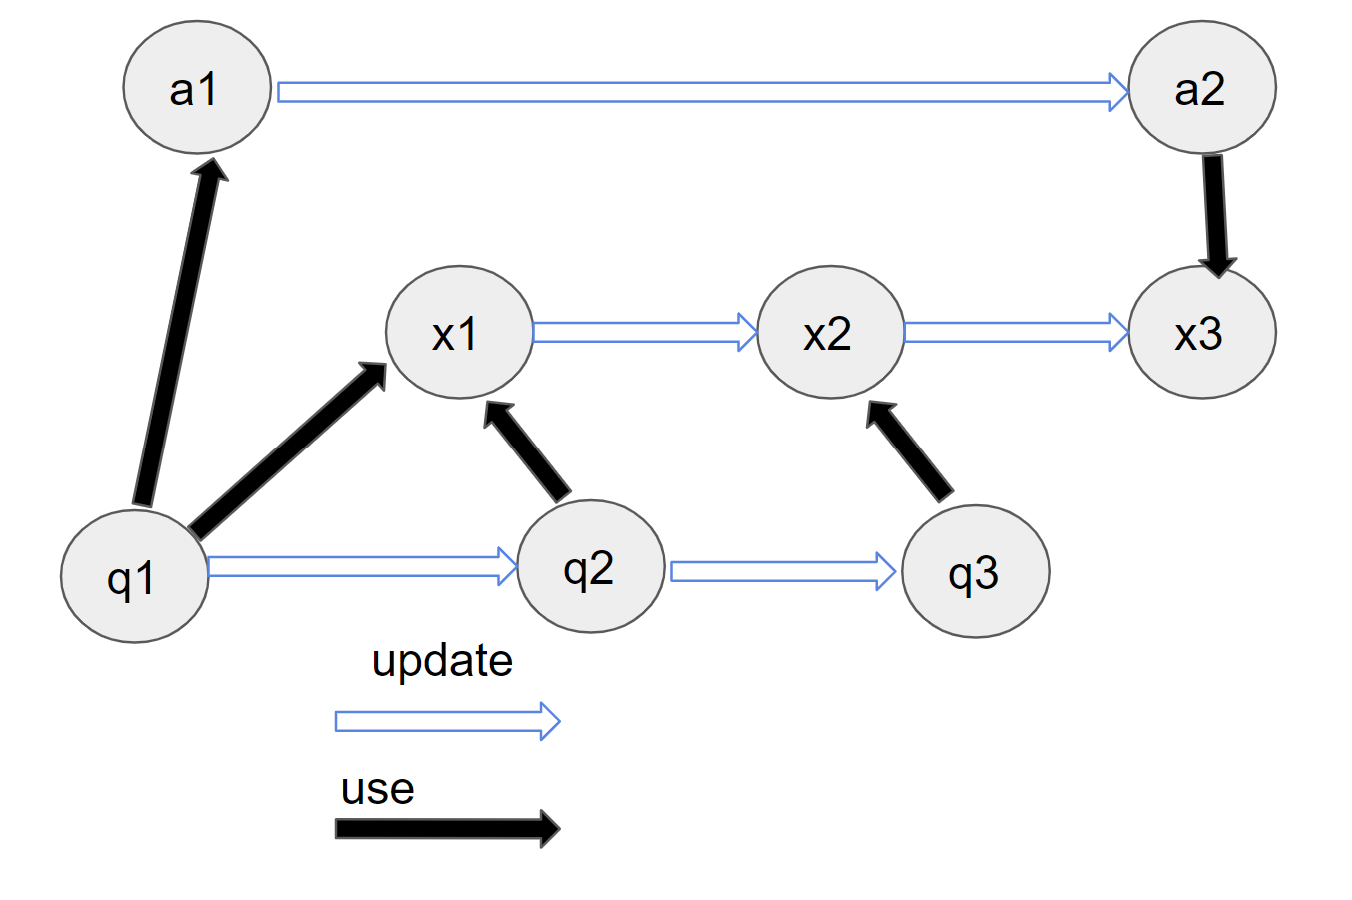
\includegraphics[width=.7\textwidth]{book/chapter-promisesandperils/pics/UniversalExample.jpg}
	\caption{Conceptual example of the Software Universe Graph, depicting the use and update relationships between different software units.}
	\label{fig:SUG}
\end{figure*}
%%%%%%%%%%%%%%%%%%%%%%%%%%%%%%%%%%%%%%%%%%%%%


\paragraph{\textbf{Component-based Representation as a Software Universe Graph}}
\label{PPM:sec:SUG}

First introduced by Kula et al.~\cite{KulaSANER18}, the \textit{Software Universe Graph} (SUG) is a structural abstraction of the software ecosystem of third-party libraries.
Figure \ref{fig:SUG} provides an illustration of the different relationships within the graph.
Let $G= (N,E)$ represent a graph $G$. $N$ is a set of nodes, each node representing a software unit. 
We define a software unit as a version instance of any software program. 

The authors then present the \textit{use} and \textit{update} relationships that exist in the ecosystem.
Hence, the edges $E$ are composed of $E_{use}$ and $E_{update}$. $E_{use}$ is a set of \textit{use-relations} and $E_{update}$ is a set of \textit{update-relations}.

\begin{definition}
An edge $u \rightarrow v \in E_{use}$ means that $u$ uses $v$. The defined functions of $E_{use}$ are:

\begin{equation}
\small
\small \use(u)\equiv \{v|u \rightarrow v\}
\normalsize
\end{equation}
\begin{equation}
\small
\small \useBy(u)\equiv \{v|v \rightarrow u\}
\normalsize
\end{equation}
\end{definition}

Use-relations can be extracted from either the source code or configuration files. 
As shown in Figure \ref{fig:SUG}, node $a1$ uses node $x1$. 
In addition, node $x1$ is used by nodes $a1$, $q1$, and $q2$. Parallel edges for node pairs are not allowed.

\begin{definition}
We represent an update relation from node $a$ to $b$ using $ a \Rightarrow b $, which means that the newer update $b$ was released from node $a$ and is defined as:
\begin{equation}
\small a \Rightarrow b \in E_{update}
\end{equation}
\end{definition}

Update relations refer to when a successive release of a software unit is made available. Figure \ref{fig:SUG} shows that node $q1$ is first updated to node $q2$. Later, node $q2$ is updated to the latest node $q3$. Hence, $q1 \Rightarrow q2 \Rightarrow q3$.
Note that an update should not be confused with forking. 
We distinguish a fork as a separate software unit. 
Each node in the SUG should be denoted by three attributes: \texttt{<name,release,time>}.  
For a node $u$, we define:

\begin{itemize}
	\item \textbf{u.name} Name is the string representation identifier of a software unit.
	We introduce the name axiom: For nodes $u$ and $v$, if $u \Rightarrow v$, then $u.name = v.name$ holds.
	
	\item \textbf{u.release}. Release refers to the specific assigned change reference for a software unit. For nodes $u$ and $v$, if $u \Rightarrow v$
	then $v$ is the immediate successor of $u$. Note that the versioning pattern may vary from project to project. 
	\item \textbf{u.time}. Time refers to the time stamp at which node $u$ was released. For nodes $u$ and $v$ of $u \Rightarrow v$, $u.time < v.time$.
\end{itemize}

\begin{figure}
	\centering
	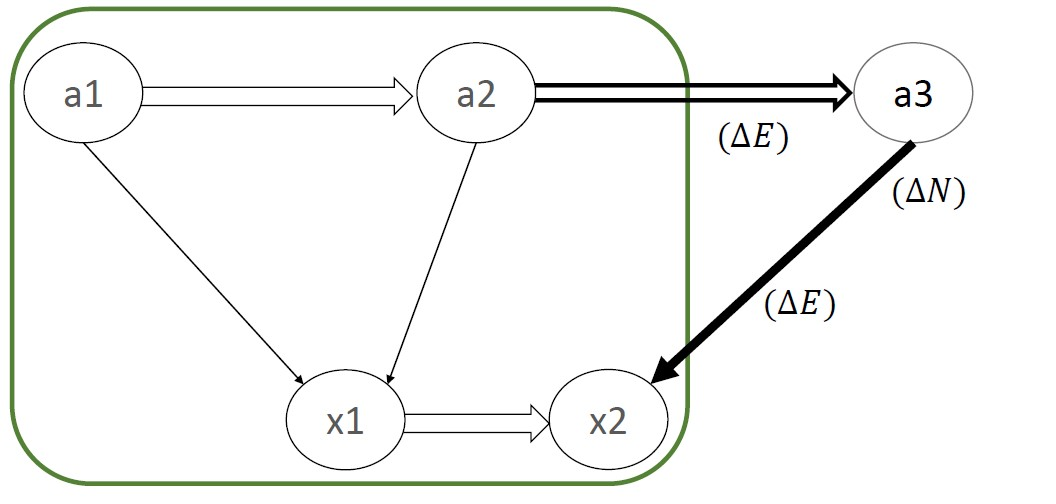
\includegraphics[width=.8\textwidth]{book/chapter-promisesandperils/pics/TemporalSUG.jpg}
	\caption{Temporal property of the SUG}
	\label{fig:SUGTemp}
\end{figure}

\begin{definition}
    
	The SUG has temporal properties.
This describes the simultaneity or ordering in reference to time. Let SUG $G = (N, E) $ be at time $t$. At time $t^{\prime} > t$, we observe an extension of $G$, such that:

\begin{equation}
\small G^{\prime} = (N \cup \Delta N, E \cup \Delta E)
\end{equation}
where $\Delta E \cap (N \times N) = \emptyset$
\end{definition}

Figure \ref{fig:SUGTemp} illustrates the temporal properties of the SUG. 
Here, it is observed that $G'$ is composed of $G$ augmented with newly added node $a3$ and its corresponding $a3 \rightarrow x2$ and $a2 \Rightarrow a3$ relations.
A SUG grows monotonically over time with only additions.
Here, we consider that modification or deletion changes on the SUG do not occur. 

\begin{definition}
    A timed SUG specifies the state of the SUG at any point in time.
So for an SUG $G=(N,E)$, we represent a timed SUG $G_{t}$ at time $t$ as a sub-graph of $G$. Formally,
\begin{equation}
\small G_t\equiv(N_{t}, E_{t})
\end{equation}
where $N_{t} = \{u|u \in N, u.time \leq t \}$ and $E_t = \{ e | e \in E \wedge e \in  N_t \}$
\end{definition}
	


\section{Data Sources}
Researchers can use various datasets to model the ecosystem using the SUG model of usage and update relationships.
The most obvious data source that has revolutionised data mining in the software engineering domain is the GitHub platform. 
Established in 2008, and then purchased by Microsoft in 2020, GitHub is home to various popular Open Source Software. 
GitHub is built on the git version control system and is useful for storing all changes made to a repository. 
In the case of the SUG, a GitHub repository can represent one software unit, whose depend relations can be extracted via a configuration file (such as the package.json file for JavaScript projects).
The repository should also contain the release information that holds the update relations.
Due to its large size, researchers and the GitHub team have made available datasets for researchers to mine, for example through the GitHub API/Graph QL.\footnote{\url{https://docs.github.com/en/graphql}} This is the backend Application Programming Interface (API) that can be used to query large amounts of data on GitHub. Most researchers use the API to download and mine information from the GitHub platform. 
It is important to note that while GitHub introduced a new feature of Dependency Graphs to map the depend relationship,\footnote{\url{https://docs.github.com/en/code-security/supply-chain-security/understanding-your-software-supply-chain/about-the-dependency-graph}} most older projects do not have this feature.
In this case, the researcher would need to manually extract and query the configuration files for dependency information. 

We refer to the first chapter for additional information on data sources for mining software ecosystems. 

\section{Promises and Perils}
\label{PPM:sec:promisesperils}

Using the SUG model of depend and use relations and the available datasets, we can now present our promises and perils of mining ecosystem information.

\subsection{Planning What Information to Mine}

\textbf{Promise 1.}\textit{
Researchers can access and link heterogeneous data related to software package ecosystems, e.g., package registries and bug trackers.}\\

When planning what information to mine from the ecosystem, researchers do not need to limit themselves to the usage and update relationship information.
Platforms that host software repositories include other software management systems such as bug trackers.
For example, GitHub allows researchers to manage GitHub Pull Requests, Issues, and Discussions not only for one project, but for multiple projects.
GitHub provides three management systems that are related to a software repository:

\begin{itemize}
    \item \textit{GitHub Discussions}\footnote{\url{https://docs.github.com/en/discussions}} - The GitHub Discussions forum is a collaborative communication forum for the community around an open source or internal project. Community members can ask and answer questions, share updates, have open-ended conversations, and follow along on decisions affecting the community's way of working.
    \item \textit{GitHub Pull Requests}\footnote{\url{https://docs.github.com/en/pull-requests}} - Pull Requests allow other developers from an ecosystem to make a contribution to a software repository. Pull requests also allow maintainers to discuss and review potential changes with collaborators and add follow-up commits before changes are merged into the software.
    \item \textit{GitHub Issues}\footnote{\url{https://docs.github.com/en/issues}} - Issues are used to track ideas, feedback, tasks, or bugs for work on GitHub.
\end{itemize}

These three systems are examples of how developers contribute to both their own and other projects. 
Hence, to incorporate this information, we can extend the SUG model, creating a model that includes a contribution relationship \cite{wattanakriengkrai2022giving}.

% Note that other platforms may also have management systems, like GitLab, BitBucket and Eclipse.

\begin{definition}
	A Dependency-Contribution graph incorporates contributions by developers whose libraries are involved in dependency relationships. 
\end{definition}

In this work \cite{wattanakriengkrai2022giving}, the authors explore the congruence between dependency updates and developer contributions, based on the original concept of social-technical congruence \cite{stcCataldo2008} where developers contribution patterns are congruent with their coordination needs. Hence, the goal is to identify contributions that are congruent to dependency updates.
As shown in Figure \ref{fig:lib} the authors extend from the typical SUG graph model where $lib_i$ depends (use) on  $lib_k$ and  $lib_j$, while  $lib_j$ also depends on $lib_k$, to the example shown in Figure \ref{fig:dc-graph}.
Different to the SUG, the graph captures developers and their contributions (i.e., the square as $dev_x$ and $dev_y$ represent two different developers making a contribution).
Here contributions are defined as $c$ (Pull Request or Issue) that were submitted to both a library and the client that depends on that library.
Hence, the graph can show contributions that are congruent to dependency changes for a software unit. 

\begin{figure}[t]
     \centering
     \begin{tikzpicture}[
         roundnode/.style={circle, fill=black, minimum size=5mm},
        squarenode/.style={fill=black, text=red, minimum size=5mm},
     ]
    \begin{scope}
         \node[roundnode, label=above:$lib_i$] (s2_proji) at (3, 2.5) {};
        \node[roundnode, label=below:$lib_j$] (s2_projj) at (4,0) {};
         \node[roundnode, label=below:$lib_k$] (s2_projk) at (2,0) {};
     \end{scope}

     \begin{scope} [every edge/.style={draw=gray, very thick}]
         \path [->] (s2_proji) edge (s2_projj);
         \path [->] (s2_proji) edge (s2_projk);
         \path [->] (s2_projj) edge (s2_projk);
     \end{scope}
     \end{tikzpicture}
    
     \caption{Example dependency graph for a given time period}
     \label{fig:lib}
     \vspace{2ex}
 \end{figure}
\begin{figure}[t]
    \centering

    \begin{tikzpicture}[
        roundnode/.style={circle, fill=black, minimum size=5mm},
        squarenode/.style={fill=black, text=red, minimum size=5mm},
    ]
    \begin{scope}
        
        \node[roundnode, label=right:$lib_i$] (s2_proji) at (4, 1.5) {};
        \node[roundnode, label=below:$lib_j$] (s2_projj) at (5,0) {};
        \node[roundnode, label=below:$lib_k$] (s2_projk) at (3,0) {};
        
        \node[squarenode, label=below:$dev_x$] (s3_devx) at (2, 3.5) {};
        
        \node[squarenode, label=below:$dev_y$] (s3_devy) at (6, 3.5) {};
        
    \end{scope}

    \begin{scope} [every edge/.style={draw=gray, very thick}]
        \path [->] (s2_proji)  edge  (s2_projj);
        \path [->] (s2_proji) edge (s2_projk);
        \path [->] (s2_projj) edge (s2_projk);
        
    \end{scope}
    \begin{scope} [every edge/.style={draw=gray, thick, double distance=2pt}]
        \path [->] (6, 2.8) edge node[left = 2mm] {$contribute$} (s2_proji);
        \path [->] (6, 2.8) edge[bend left=15] node[right = 1mm] {$contribute$} (s2_projj);
        \path [->] (2, 2.8) edge node[right = 2mm] {$$} (s2_proji);
        \path [->] (2, 2.8) edge[bend right=15] node[left = 1mm] {$contribute$} (s2_projk);
    \end{scope}
    \end{tikzpicture}
\end{figure}
\begin{figure}[t]
    \centering
    \begin{tikzpicture}[
        roundnode/.style={circle, fill=black, minimum size=5mm},
        squarenode/.style={fill=black, text=red, minimum size=5mm},
    ]
    \end{tikzpicture}
\caption{Example Dependency-Contribution graph showing relationships between contributions and dependencies}
 \label{fig:dc-graph}
\end{figure}

This is just one example of the type of research that is enabled by access to heterogeneous data related to software package ecosystems.

\smallskip\noindent\textbf{Peril 1.}\textit{
 Developers might use different identifiers when contributing to different parts of a software package ecosystem, e.g., when contributing to different libraries.}\\
 
When modelling using such graphs, there is a threat that contributors may use multiple identifiers (i.e., $c_x$ and $c_y$ are the same contributor).
This is a well-known research problem, and there has been work to merge these accounts, such as \cite{wiese2016mailing}.
GitHub has introduced mechanisms such as two-factor authentication\footnote{\url{https://docs.github.com/en/authentication/securing-your-account-with-two-factor-authentication-2fa/configuring-two-factor-authentication}} to counteract the issue of multiple identifiers.
This is since developers might be less likely to switch accounts if it requires cumbersome authentication.


\smallskip\noindent\textbf{Peril 2.}\textit{
Developers' contributions to software package ecosystems might be interspersed with bot contributions, e.g., automated dependency updates.}\\

The rise of automation and artificial intelligence has led to much work on the integration of automated scheduling (i.e., bots) into software development workflows \cite{Storey2016, Farooq2016, Wessel2018, Erlenhov2019, bot_modify_wf} to name a few. These bots are designed to perform specific tasks within a software package ecosystem. For example, a bot may be programmed to automatically update dependencies, test code changes, or deploy software to production. As an example, the Google APIs repo-automation-bots project lists bots for automated labelling of issues and pull requests, automated approval of pull requests, and triggering releases.\footnote{\url{https://github.com/googleapis/repo-automation-bots}}
Bots perform common maintenance tasks in many software projects and are now commonplace \cite{Beschastnikh2017, Urli2018,BIMAN,bot_or_not}.
Especially with bots such as dependabot (automated pull requests to update configurations to reduce the risk of vulnerability threats),\footnote{\url{https://github.com/dependabot}} more and more automation has caused a lot of noise in the contributions between projects.
There are also bots for communication and documentation \cite{Urli2018, Lin2016, Lebeuf2017a}.

To be able to draw accurate conclusions about what humans are doing in software package ecosystems, researchers should consider distinguishing between bot and human contributions.
It is also important to differentiate this from other contributions \cite{maeprasart2022understanding}.
The research community has responded well, with a wide range of techniques and tools to mitigate this peril \cite{Bodegha2021, golzadeh2022accuracy}.

\smallskip\noindent\textbf{Peril 3.}\textit{
Not all developer activities in software package ecosystems are accessible to the public, e.g., library use in proprietary settings.
}\\

Not all developer activities in software package ecosystems are accessible to the public, e.g., when the boundary between open source and industry is blurred \cite{stol2014inner}, which presents a challenge for researchers who aim to study the development process. This is particularly true in proprietary settings where software development is performed behind closed doors or is open source for a limited time period, thus resulting in the artefacts not permanently being publicly available.
This can make it difficult to understand the broader ecosystem in which a software project is developed.
Proprietary settings may lead to non-standardisation in software development practises. Different software projects may use different management systems and tools, making it difficult to accurately compare and analyse software development activities across various projects. For example, some projects may use communication, documentation, and other management tools not captured on the same platform \cite{montgomery2022alternative}. For example, some projects might use Bugzilla instead of issues and pull requests for their bug and code review systems, while others may use Discord, Slack channels, or email threads for their communication needs.

This lack of standardisation in software development practises presents a challenge for researchers who study the software package ecosystem and understand the development process. To address this issue, researchers should strive to collect data from a diverse set of projects to gain a comprehensive understanding of the software package ecosystem. In addition, researchers may need to adjust their methodologies or data collection techniques to accommodate the different tools and practises used by different software projects.

\subsection{Defining Components and their Dependencies}

\smallskip\noindent\textbf{Promise 2.}\textit{
Researchers can access a software package ecosystem's dependency network through package managers and registries, e.g., npm lists the dependencies and dependents for over a million libraries.}\\


With the rise of curated datasets like libraries.io, researchers can now recover and model dependency relations between software units using pre-extracted datasets.
Table \ref{tab:PM_features} shows examples of popular package managers mined from the libraries.io dataset in 2020. 

\begin{table*}[]
\caption{Summary of 13 package managers from libraries.io as ranked by TIOBE in 2020}
 \label{tab:PM_features}
 \centering
\begin{tabular}{@{}llrlll@{}}
\toprule
\begin{tabular}[c]{@{}l@{}}Package \\ Ecosystem\end{tabular} & \begin{tabular}[c]{@{}l@{}}Programming \\ Language\end{tabular} &  \begin{tabular}[c]{@{}l@{}}Tiobe \\ Rank\end{tabular} & Environment & \begin{tabular}[c]{@{}l@{}}Dependency \\ Tree\end{tabular} & \begin{tabular}[c]{@{}l@{}}Package   \\Archive link\end{tabular}\\ \midrule
PyPI & Python & 2 & Python & Flat & pypi.org  \\
Maven & Java & 3 & JVM & Flat & Maven.org  \\
Bower & JavaScript & 7 & Node.js & Flat & bower.io  \\
Meteor & JavaScript & 7 & Node.js & Nested & atmospherejs.com \\
npm & JavaScript & 7 & Node.js & Nested (v2) & npmjs.com  \\
Packagist & PHP & 8 & PHP & Flat & packagist.org \\
Puppet & Ruby & 13 & Ruby MRI & Flat & forge.puppet.com  \\
RubyGems & Ruby & 13 & Ruby MRI & Flat & rubygems.org  \\
CRAN & R & 14 & RStudio & Flat & cran.r-project.org  \\
CPAN & Perl & 15 & Perl & Flat & metacpan.org  \\
GO & Golang & 20 & Go & Flat & pkg.go.dev  \\
NuGet & C\#, VB & 5, 6 & .NET & Flat & nuget.org \\
Anaconda & Python, R, C\# & 2, 14, 5 & Anaconda & Flat & anaconda.org  \\ \bottomrule
\end{tabular}
\end{table*}

\smallskip\noindent\textbf{Peril 4.}\textit{
Different software package ecosystems define the concept of ``dependency'' differently, e.g., by allowing or not allowing different versions of a library on the same dependency tree.
}\\

Different software package ecosystems have varying definitions of what constitutes a dependency. For example, some ecosystems may allow multiple versions of a library to exist on the same dependency tree, while others may restrict developers to a single version of a library \cite{Islam}. These restrictions are often based on the programming language being used, as different languages have different approaches to managing dependencies. It is important to consider the restrictions on dependency relationships when studying software package ecosystems, as they can have a major impact on the development process. For example, the ability to use multiple versions of a library on the same dependency tree can greatly simplify the process of updating dependencies and can make it easier to resolve conflicts between libraries.

One way to visualise the impact of these restrictions is to compare the difference between a nested dependency tree and a directed dependency tree, as shown in Figure \ref{fig:nest}.\footnote{Taken from \url{https://npm.github.io/how-npm-works-docs/npm3/how-npm3-works.html}} This distinction is important because it highlights the different ways that a software unit can depend on different versions of the same library.
In this example, npm v3 creates the dependency tree based on the installation order, therefore flattening unnecessary nested dependencies (i.e., B v1.0 in cyan). This reduces the complexity of a nested tree by resolving some of the transitive dependencies (nested dependencies).

\begin{figure}
	\centering
	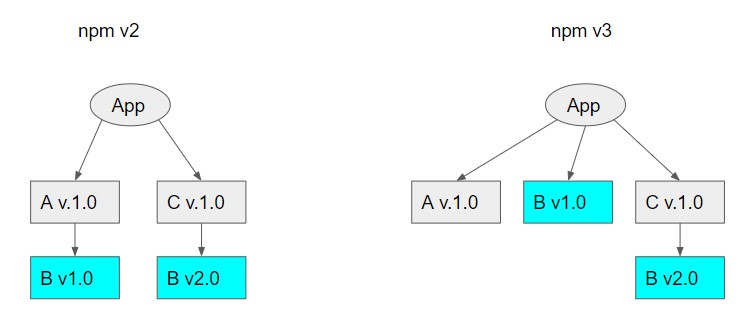
\includegraphics[width=.8\textwidth]{book/chapter-promisesandperils/pics/nestedv2.jpg}
	\caption{Difference between flat and nested dependencies}
	\label{fig:nest}
\end{figure}

\smallskip\noindent\textbf{Peril 5.}\textit{
Developers might declare a dependency to other parts of a software package ecosystem but not use it, e.g., because they failed to update its removal.
}\\

It is common for developers to declare dependencies on other parts of the software package ecosystem but not always use them. This can happen for various reasons, such as forgetting to remove the dependency after it is no longer needed. This can pose a challenge for researchers who are trying to extract dependencies from package managers, like those in configuration files, as there may be inconsistencies between the listed dependencies and what is actually being compiled and used by the code. This can lead to a biased understanding of the software package ecosystem and the relationships between software components.

To address this issue, there have been numerous efforts to track the actual library dependencies compiled and executed in software systems. These efforts aim to provide a more accurate understanding of the dependencies and the relationships between software components. For example, research has been conducted on the use of dynamic analysis to track compiled dependencies in real time and on the development of tools to automatically detect and track executed dependencies \cite{Zapata:ICSME2018, Ponta2018,Chinthanet:ASE2020}.

\subsection{Defining Boundaries and Completeness}

\smallskip\noindent\textbf{Promise 3.}\textit{
Researchers can use the boundaries of software package ecosystems to study communities of developers, e.g., developers contributing to and/or benefiting from the npm ecosystem.
}\\

Following Promise 2, the emergence of package managers has also led to studies that approximate software communities.
Using the libraries.io dataset, researchers were able to study projects that host libraries that use package managers.
Researchers have used this dataset to compare different library ecosystems \cite{kikas.2017,decan:emse:2019,CogoDown2019}.


\smallskip\noindent\textbf{Peril 6.}\textit{
Package managers do not always represent software package ecosystems, their communities, or their sub-communities, e.g., in cases where multiple package managers exist.
}\\

Package managers are a fundamental aspect of software package ecosystems, but do not always fully represent the complex relationships and interactions that occur within a community of developers and users, as shown in Table~\ref{tab:PM_features}. In some cases, multiple package managers exist for the same programming language, creating a complex landscape of software libraries and dependencies that are not always easily understood. For instance, Bower and Meteor manage npm libraries, which can lead to confusion and overlap in the management of dependencies.

Similarly, Java, Scala, Android, and other Java-based open source communities all use the Maven package manager, but each of these communities has its own unique set of libraries, dependencies, and development practises. Researchers should be aware of the limitations of package managers when studying software package ecosystems, and consider the broader context and relationships that exist within these communities. 

\smallskip\noindent\textbf{Peril 7.}\textit{
Lack of activity in parts of a software package ecosystem does not necessarily indicate project failure, e.g., when highly depended-upon libraries are feature-complete.
}\\

It is important to note that lack of activity in a part of a software package ecosystem does not always mean project failure \cite{coelho2017modern}. In some cases, highly relied-upon libraries that have reached feature-completeness may see little activity, but continue to be used by the software community. 

However, it is still important to consider the long-term sustainability of these libraries, especially given the rate at which technology and software development practises change. This has become a topic of interest in recent years, and researchers have explored best practises for sustaining open source projects and ensuring their continued success \cite{Ait2022,valiev2018ecosystem}. Understanding the factors that contribute to project sustainability is important to ensure the longevity and continued growth of software package ecosystems.

\smallskip\noindent\textbf{Peril 8.}\textit{
Sampling from a software package ecosystem is challenging since sub-setting might alter the dependency network, e.g., by breaking dependency chains.
}\\

Sampling from a package ecosystem is not straightforward, as the sample composition can be significantly affected due to missing dependency links between libraries. For instance, a subset of the ecosystem might alter the dependencies between libraries, leading to the breakdown of the dependency chains. This could lead to an incomplete picture of the software package ecosystem, leading to incorrect conclusions from a study. To minimise this risk, researchers should carefully consider the boundaries of their study and choose the appropriate sampling method based on the research questions and goals. For example, researchers could focus on popular, highly dependent, or risk-vulnerable aspects of the ecosystem as a starting point. 
For some ecosystems, the number of downloads, GitHub stars, and watchers are other aspects for the researcher to utilise.


\smallskip\noindent\textbf{Peril 9.}\textit{
Sampling from a software package ecosystem is challenging since the dependency network changes over time, e.g., when dependencies are added, removed, upgraded, or downgraded.
}\\

The dynamic nature of package ecosystems and the constant changes to their dependencies can impact the generalisability of the results. Therefore, it is important to also consider the time granularity of the analysis. For example, if the goal is to understand the evolution of dependencies over time, a finer time granularity may be necessary to capture the smaller changes and trends. However, if the goal is to understand the overall structure and relationships within the ecosystem, a coarser time granularity may be sufficient. Based on recent studies \cite{wattanakriengkrai2022giving,valiev2018ecosystem,Mirsaeedi:icse2020, Brindescu:emse2020, Nassif:icsme2017}, a three-month window seems appropriate for some studies.
Another level of granularity to consider is the size of the component. For instance, there are cases where a single package may contain more than one repository, especially for large library frameworks. 
The granularity also depends on the nature of the ecosystem itself. For instance, researchers should understand whether the ecosystem comprises library packages (e.g., PyPI), plugins (e.g., Eclipse), or is a library distribution (e.g., Android).



\subsection{Analysing and Visualising the Data}

\textbf{Peril 10.}\textit{
Analysing and visualising entire software package ecosystems is challenging due to their size, e.g., in terms of nodes and edges in the network.
}\\

The size of software package ecosystems implies large data sets, which can be overwhelming for tools and algorithms to analyse and display. Therefore, it may be necessary to make choices about the granularity of the data included in the analysis and visualisation. Another alternative is to focus on the most critical parts of the software package ecosystem, such as the high-level structure, highly dependent packages, or parts of the system that pose a risk to security and reliability. 
The key is to strike a balance between detail and simplicity, providing a meaningful representation of the ecosystem while being able to handle the complexity of its size.


\section{Application: When to Apply Which Peril}
\label{PPM:sec:application}

We include a disclaimer stating that not all perils are applicable to every mining situation. To demonstrate the practical application of our perils and their mitigation, we present two case studies that involve mining the software package ecosystem. Each case study has a distinct research objective and focusses on a specific dataset to be mined.

\subsection{Two Case Studies}
Table \ref{tab:cases} presents the two case studies we have selected for this analysis.
The \textit{first case} involves mining for contributions congruent to dependency updates \cite{wattanakriengkrai2022giving}. 
In this work, the authors mine GitHub repositories for Pull Requests and Issues that were submitted and merged congruent to dependency updates within the npm ecosystem. 
The \textit{second case} involves mining communication data for the Eclipse ecosystem \cite{Nugroho2021}. Although the second case does not mine for dependency relations (i.e., use relations),  we show that these perils still apply when mining for other relationships in an ecosystem.
Moreover, the second case studies the Eclipse ecosystem, which is a different dataset compared to the more popular GitHub dataset.

\subsection{Applying Perils and their Mitigation Strategies}
Table \ref{tab:perilsapp} provides a summary of the perils that can be applied to each of the case studies. We will now go into the details of mitigation strategies based on these perils. 
For better organisation and understanding, we have grouped the perils according to the four logical processes for mining.

\smallskip\noindent\textbf{Information to Mine}. 
The first set of mitigation strategies, which addresses perils 1-3, focusses on planning which information to mine. There are two primary strategies that researchers can employ:


\begin{enumerate}
    \item Researchers should use research tools and techniques to remove noise and other biases in the dataset, such as bot detection and the handling of multiple identities. This strategy was implemented in both case studies, as contributions and discussions often have the potential to involve bots or developers with multiple identities.
\item Depending on the research goals, researchers should recognise that not all contributions are equal and filter the dataset accordingly.
\end{enumerate}

We applied these two strategies to both cases. In the first case, the goal was to capture all congruent contributions, so we filtered out contributions made to libraries without dependencies. Since all npm packages are listed in the registry, Peril 3 (private activities) did not apply.
In the second case, we addressed Peril 1 by conducting a qualitative analysis to ensure that the member identities were not duplicated, as Eclipse developers were known to change identities. To mitigate Peril 2, we removed bot responses. For the second case, since all forum data is made public, Peril 3 did not apply.


\begin{table}
\centering
\caption{Description of the research objectives and datasets for the case studies}
 \label{tab:cases}
\begin{tabular}{lp{5cm}r} 
\toprule
\textbf{Case Study} & \textbf{Research Objective}                                                          & \textbf{Datasets}           \\
\midrule
Wattanakriengkrai \etal \cite{wattanakriengkrai2022giving}             & Explore code contributions between library and client (i.e, use-relations)  & libraries.io\\
& &  GitHub API \\
Nugroho \etal \cite{Nugroho2021}                & Explore discussion contributions between contributors (i.e., contributions) & Eclipse API                \\
\bottomrule
\end{tabular}
\end{table}

\begin{table}
\centering
\caption{Application of each peril to the case studies}
 \label{tab:perilsapp}
\begin{tabular}{rp{8cm}ccc} 
\toprule                   
& \textbf{Perils}       & case 1      & case 2                 \\
                                                                               & & npm  & Eclipse   \\
\midrule
\textbf{P1} &Developers might use different identifiers when contributing to different parts of a software package ecosystem, e.g., when contributing to different libraries.                             &    \CheckedBox         &          \CheckedBox           \\ 
%\hline
\textbf{P2} & Developers' contributions to software package ecosystems might be interspersed with bot contributions, e.g., automated dependency updates.                                                      &      \CheckedBox               &      \CheckedBox               \\ 
%\hline
\textbf{P3} & Not all developer activities in software package ecosystems are accessible to the public, e.g., library use in proprietary settings.                                                         &         -           &      \CheckedBox               \\ 
%\hline
\textbf{P4} & Different software package ecosystems define the concept of \`{}\`{}dependency'' differently, e.g., by allowing or not allowing different versions of a library on the same dependency tree. &         \CheckedBox       &     -                            \\ 
%\hline
\textbf{P5} & Developers might declare a dependency to other parts of a software package ecosystem but not use it, e.g., because they failed to update its removal.                                        &     -           &  -    \\
%\hline
\textbf{P6} &Package managers do not always represent software package ecosystems, their communities, or their sub-communities, e.g., in cases where multiple package managers exist.                     &     -                   &  -                  \\
%\hline
\textbf{P7} & Lack of activity in parts of a software package ecosystem does not necessarily indicate project failure, e.g., when highly depended-upon libraries are feature-complete.                     &       \CheckedBox         &  -                           \\
%\hline
\textbf{P8} &Sampling from a software package ecosystem is challenging since sub-setting might alter the dependency network, e.g., by breaking dependency chains.                                         &        \CheckedBox        &     \CheckedBox                                \\
%\hline
\textbf{P9} &Sampling from a software package ecosystem is challenging since the dependency network changes over time, e.g., when dependencies are added, removed, upgraded, or downgraded.               &       \CheckedBox         &     -                          \\
%\hline
\textbf{P10} &Analysing and visualising entire software package ecosystems is challenging due to their size, e.g., in terms of nodes and edges in the network.                                  &        \CheckedBox      &      \CheckedBox               \\
\bottomrule
\end{tabular}
\end{table}

\smallskip\noindent\textbf{Defining Dependencies}. 
The second set of perils (Perils 4-5) is related to dependency relationships between software units, and only the first case study is applicable. To address these perils, researchers should adopt the following strategy:

\begin{enumerate}
    \item Researchers should not rely solely on listed dependencies in configuration files (e.g., pom.xml, package.json, etc.) as a measure of dependency between two components. Instead, code-centric approaches should be used to validate which libraries are actually depended upon.
\end{enumerate}

For example, in the first case, in addition to mining the configuration information, the authors also analysed the similarity of the source code contributions to address Peril 4. Regarding Peril 5, since the study's objective was to investigate changes to the configuration files, the risk of the update not being executed was deemed less important.
It is important to note that the second case study did not include dependency analysis and, therefore, these perils did not apply.

\begin{figure*}[]
    \centering
    \begin{subfigure}{0.9\linewidth}
         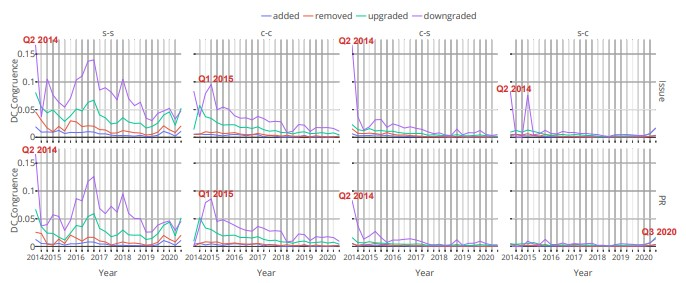
\includegraphics[width=1.1\textwidth]{book/chapter-promisesandperils/pics/congruentViz.jpg}
         \caption{Visualization of a Time analysis for 107,242 libraries.}
     \end{subfigure}
     \begin{subfigure}{0.9\linewidth}
         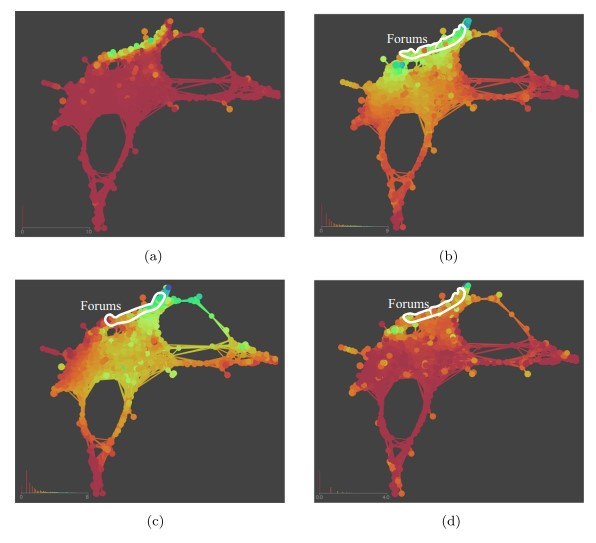
\includegraphics[width=1\textwidth]{book/chapter-promisesandperils/pics/eclipseViz.jpg}
         \caption{A Visual Topology map for 832,058 threads}
     \end{subfigure}
    \caption{Visualisation examples for the two case studies}
    \label{fig:visCase}
\end{figure*}

\smallskip\noindent\textbf{Defining Boundaries}.
The third set of perils (Perils 6-9) is related to the definition of boundaries and completeness and is relevant for both case studies. To mitigate these perils, we recommend the following strategies:

\begin{enumerate}
    \item Researchers should recognise that a dormant project does not necessarily mean that it is inactive. Instead, studies can use alternative heuristics, such as the number of dependents and dependencies, as better indicators of a project's importance in the ecosystem.
    \item Researchers should not rely solely on the programming language to define sub-communities. Using a common package manager for the programming language is a more effective rule of thumb for distinguishing boundaries.
    \item Researchers should avoid random sampling. Instead, sampling should be tailored to the research goals by considering factors such as an appropriate time window or focussing on specific attributes of components (e.g., most dependents, most popular, most contributors).
\end{enumerate}


Peril 6 did not apply to any of the case studies. 
Particularly for the first case, since the goal was to explore the npm package ecosystem, we assumed that the boundaries were clearly defined by the npm registry. 
Similarly, the second case study used the generic Eclipse platform as the boundary. 
Peril 7 was applied to the npm study, while Peril 8 was applied to both case studies. 
As a result, the two cases conducted a qualitative analysis of the dataset to gain deeper insights.
In the first case study, a three-month time window was created to capture dependencies. 
For the second case study, forum contributors were sampled into three groups (i.e., junior, member, or senior) according to the sliding window of their contributions. 

\smallskip\noindent\textbf{Visualisation}.
The final peril (Peril 10) relates to visualisation, which can be challenging due to the vast size and complexity of software ecosystems. As it is not feasible to visualise every aspect of an ecosystem simultaneously, a focused approach is necessary. A mitigation strategy is to select specific attributes of the ecosystem (e.g., the most dependent, most popular, and most contributions) that align with the research needs and objectives. 

Figure \ref{fig:visCase} shows two cases where visualizations are employed to gain insights, especially for large datasets.
In the first figure (a), we visualize the distributions of the data set and applied the appropriate statistical tests, along with the effect size, to test our hypotheses and answer research questions. 
In the second example (b), although not directly related to package ecosystems, the authors utilized a topological visualization \cite{Lum2013ExtractingIF} to gain insights on the over 800,000 forum threads of discussions. 



\section{Chapter Summary}
In this chapter, we explore the various aspects of mining information from the software package ecosystem, presenting three promises and ten perils that researchers should be aware of when undertaking such tasks. The chapter is structured around four key processes for mining: 1) Planning what Information to Mine, 2) Defining Components and their Dependencies, 3) Defining Boundaries and Completeness, and 4) Analysing and Visualising the Data. To help new and experienced researchers navigate these challenges, we introduced the SUG model, which can serve as a valuable tool to minimise threats to validity. Although some perils may be more relevant to specific research objectives, our aim is to equip researchers with the knowledge and resources needed to confidently gather and integrate software package ecosystem data into their work.
%An Introduction to Software Development Ecosystems
%Semantic labeling three-letter-code: INT (e.g. \chapter{INT})

% 
\title{Promises and Perils of Mining \\ Software Package Ecosystem Data}
\author{Raula Gaikovina Kula \and Katsuro Inoue \and Christoph Treude}
\institute{Raula Gaikovina Kula \at Nara Institute of Science and Technology, Japan, \email{raula-k@naist.jp}
\and Katsuro Inoue \at Nanzan University, Japan \email{ inoue599@nanzan-u.ac.jp}
\and  Christoph Treude \at The University of Melbourne, Australia \email{christoph.treude@unimelb.edu.au}}

\maketitle
\label{PPM:ch}
\abstract*{The use of third-party packages is becoming increasingly popular and has led to the emergence of large software package ecosystems with a maze of inter-dependencies. Since the reliance on these ecosystems enables developers to reduce development effort and increase productivity, it has attracted the interest of researchers: understanding the infrastructure and dynamics of package ecosystems has given rise to approaches for better code reuse, automated updates, and the avoidance of vulnerabilities, to name a few examples. But the reality of these ecosystems also poses challenges to software engineering researchers, such as: How do we obtain the complete network of dependencies along with the corresponding versioning information? What are the boundaries of these package ecosystem? How do we consistently detect dependencies that are declared but not used? How do we consistently identify developers within a package ecosystem? How much of the ecosystem do we need to understand to analyse a single component? How well do our approaches generalise across different programming languages and package ecosystems? In this chapter, we review promises and perils of mining the rich data related to software package ecosystems available to software engineering researchers.}

\abstract{The use of third-party packages is becoming increasingly popular and has led to the emergence of large software package ecosystems with a maze of inter-dependencies. Since the reliance on these ecosystems enables developers to reduce development effort and increase productivity, it has attracted the interest of researchers: understanding the infrastructure and dynamics of package ecosystems has given rise to approaches for better code reuse, automated updates, and the avoidance of vulnerabilities, to name a few examples. But the reality of these ecosystems also poses challenges to software engineering researchers, such as: How do we obtain the complete network of dependencies along with the corresponding versioning information? What are the boundaries of these package ecosystems? How do we consistently detect dependencies that are declared but not used? How do we consistently identify developers within a package ecosystem? How much of the ecosystem do we need to understand to analyse a single component? How well do our approaches generalise across different programming languages and package ecosystems? In this chapter, we review promises and perils of mining the rich data related to software package ecosystems available to software engineering researchers.}

%%%%%%%%%%%%%%%%%%%%%%%%%%%%%%%%%%%%%%%%%%%%%%%%%%%%%%%%%%%%%%%%%%

\section{Introduction}
\label{PPM:sec:definition}

Third-party libraries are a great way for developers to incorporate code without having to write their own for every functionality required. By using these libraries, developers can save time and energy while still getting the functions they need.
Using third-party libraries is becoming increasingly popular and has led to the emergence of large software package ecosystems such as npm. While these ecosystems offer many benefits, they also come with risks, such as software vulnerability attacks \cite{Chinthanet:ASE2020}.

Large software package ecosystems are a treasure trove for researchers who can investigate a wide range of questions. For example, by studying activity in large ecosystems, researchers can identify which libraries are the most popular and learn what characteristics make them successful \cite{kikas.2017,decan:emse:2019}.
Additionally, research on large ecosystems can help developers understand how to protect their code from malicious actors who may attempt to exploit vulnerabilities or insert malware into popular libraries.
Studying large software package ecosystems can help us better understand the dynamics of open source development in general. Open source development is a complex process that involves many different stakeholders working together (or sometimes competing) to create valuable code that anyone can use or improve upon. By understanding how these interactions play out in different types of ecosystem structures -- including those with many small projects versus few very large ones -- we can develop insights that might be applicable more broadly across other types of collaborative systems.

In this chapter, we identify and discuss promises and perils during the mining process, ranging from planning what information to mine from the ecosystem to analysing and visualising the mined data. 
Therefore, the chapter is broken down into these logical processes of mining ecosystem data: 1) Planning what Information to Mine, 2) Defining Components and their Dependencies, 3) Defining Boundaries and Completeness, and 4) Analysing and Visualising the Data.

This chapter is intended for researchers and practitioners who are interested in exploring and exploiting software package ecosystem information from a diverse range of sources that are publicly available. 
We also highlight the pitfalls to consider during the mining process, particularly when these pitfalls could lead to a misinterpretation of the analysis and results. 
The chapter is written in a manner that encourages newcomers who have little or no experience or who are interested in utilising ecosystem data across different disciplines outside of software engineering.
Our goal is to get new researchers quickly accustomed to gathering ecosystem information for their research.


\section{A Component-based Software Ecosystem}

Defined as a component-based software ecosystem, we suggest using the term `software package ecosystem' as a suitable term for the symbiotic relationships among third-party library components (as software projects or repositories), as these libraries and their dependent clients coexist on the same technological platform, therefore sharing the same environment and other internal and external factors (e.g., security threats, sharing contributions, etc.).
Please refer to the Introduction chapter for an in-depth definition of the different types of software ecosystems.
We present our interpretation of the software package ecosystem in Kula et al.~\cite{KulaSANER18}, where we formally define a package ecosystem using a Software Universe Graph (SUG).
This is modelled as a structured abstraction of the evolution of software systems and their library dependencies over time.

%%%%%%%%%%%%%%%%%%%%%%%%%%%%%%%%%%%%%%%%%%
\begin{figure*}
	\centering
	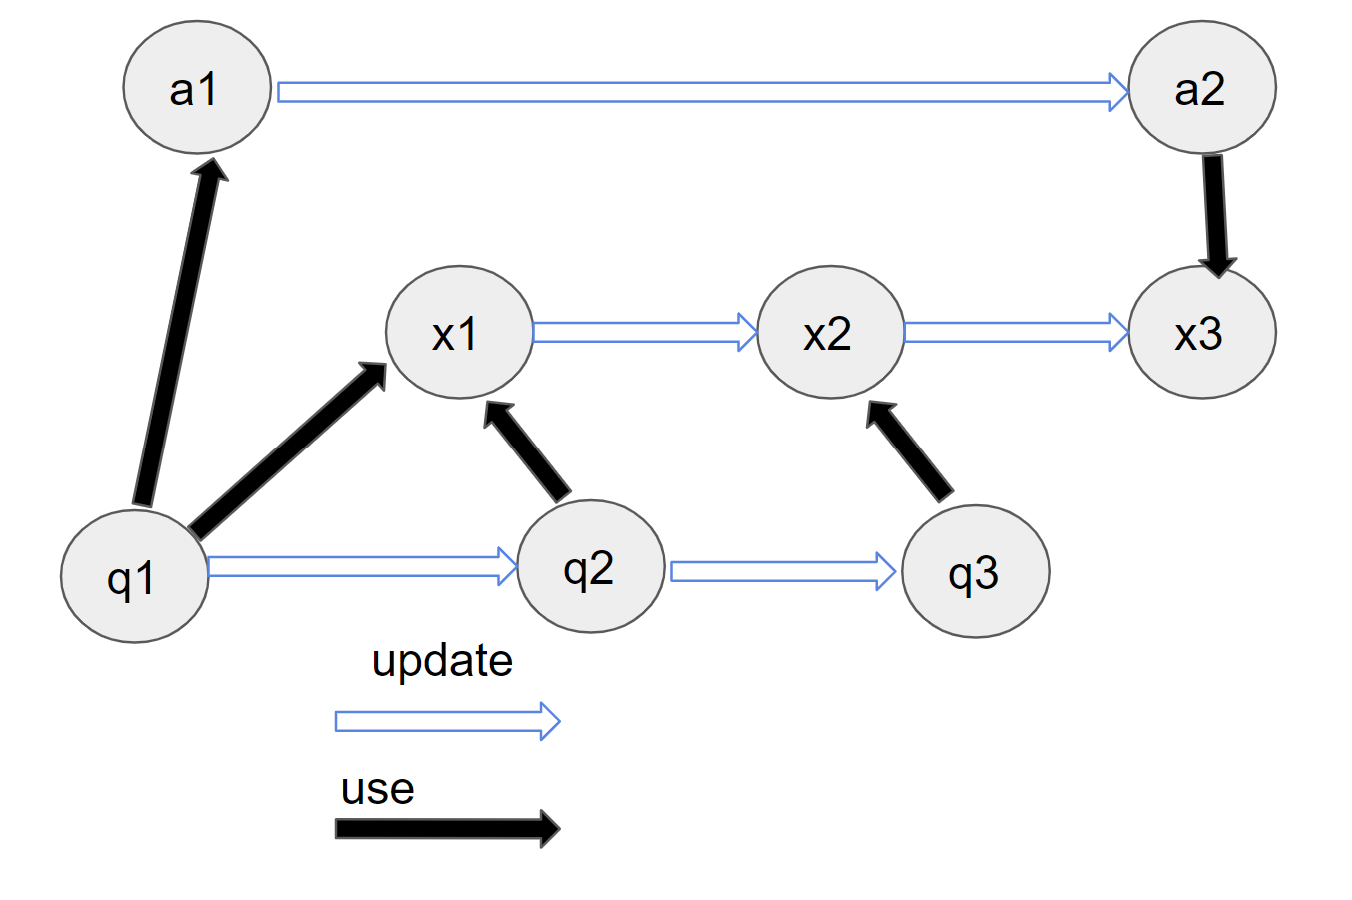
\includegraphics[width=.7\textwidth]{book/chapter-promisesandperils/pics/UniversalExample.jpg}
	\caption{Conceptual example of the Software Universe Graph, depicting the use and update relationships between different software units.}
	\label{fig:SUG}
\end{figure*}
%%%%%%%%%%%%%%%%%%%%%%%%%%%%%%%%%%%%%%%%%%%%%


\paragraph{\textbf{Component-based Representation as a Software Universe Graph}}
\label{PPM:sec:SUG}

First introduced by Kula et al.~\cite{KulaSANER18}, the \textit{Software Universe Graph} (SUG) is a structural abstraction of the software ecosystem of third-party libraries.
Figure \ref{fig:SUG} provides an illustration of the different relationships within the graph.
Let $G= (N,E)$ represent a graph $G$. $N$ is a set of nodes, each node representing a software unit. 
We define a software unit as a version instance of any software program. 

The authors then present the \textit{use} and \textit{update} relationships that exist in the ecosystem.
Hence, the edges $E$ are composed of $E_{use}$ and $E_{update}$. $E_{use}$ is a set of \textit{use-relations} and $E_{update}$ is a set of \textit{update-relations}.

\begin{definition}
An edge $u \rightarrow v \in E_{use}$ means that $u$ uses $v$. The defined functions of $E_{use}$ are:

\begin{equation}
\small
\small \use(u)\equiv \{v|u \rightarrow v\}
\normalsize
\end{equation}
\begin{equation}
\small
\small \useBy(u)\equiv \{v|v \rightarrow u\}
\normalsize
\end{equation}
\end{definition}

Use-relations can be extracted from either the source code or configuration files. 
As shown in Figure \ref{fig:SUG}, node $a1$ uses node $x1$. 
In addition, node $x1$ is used by nodes $a1$, $q1$, and $q2$. Parallel edges for node pairs are not allowed.

\begin{definition}
We represent an update relation from node $a$ to $b$ using $ a \Rightarrow b $, which means that the newer update $b$ was released from node $a$ and is defined as:
\begin{equation}
\small a \Rightarrow b \in E_{update}
\end{equation}
\end{definition}

Update relations refer to when a successive release of a software unit is made available. Figure \ref{fig:SUG} shows that node $q1$ is first updated to node $q2$. Later, node $q2$ is updated to the latest node $q3$. Hence, $q1 \Rightarrow q2 \Rightarrow q3$.
Note that an update should not be confused with forking. 
We distinguish a fork as a separate software unit. 
Each node in the SUG should be denoted by three attributes: \texttt{<name,release,time>}.  
For a node $u$, we define:

\begin{itemize}
	\item \textbf{u.name} Name is the string representation identifier of a software unit.
	We introduce the name axiom: For nodes $u$ and $v$, if $u \Rightarrow v$, then $u.name = v.name$ holds.
	
	\item \textbf{u.release}. Release refers to the specific assigned change reference for a software unit. For nodes $u$ and $v$, if $u \Rightarrow v$
	then $v$ is the immediate successor of $u$. Note that the versioning pattern may vary from project to project. 
	\item \textbf{u.time}. Time refers to the time stamp at which node $u$ was released. For nodes $u$ and $v$ of $u \Rightarrow v$, $u.time < v.time$.
\end{itemize}

\begin{figure}
	\centering
	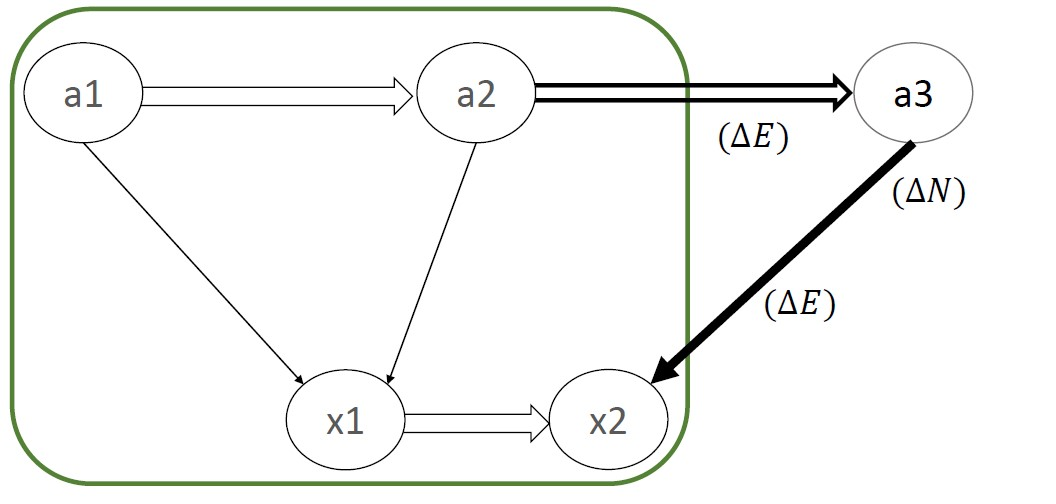
\includegraphics[width=.8\textwidth]{book/chapter-promisesandperils/pics/TemporalSUG.jpg}
	\caption{Temporal property of the SUG}
	\label{fig:SUGTemp}
\end{figure}

\begin{definition}
    
	The SUG has temporal properties.
This describes the simultaneity or ordering in reference to time. Let SUG $G = (N, E) $ be at time $t$. At time $t^{\prime} > t$, we observe an extension of $G$, such that:

\begin{equation}
\small G^{\prime} = (N \cup \Delta N, E \cup \Delta E)
\end{equation}
where $\Delta E \cap (N \times N) = \emptyset$
\end{definition}

Figure \ref{fig:SUGTemp} illustrates the temporal properties of the SUG. 
Here, it is observed that $G'$ is composed of $G$ augmented with newly added node $a3$ and its corresponding $a3 \rightarrow x2$ and $a2 \Rightarrow a3$ relations.
A SUG grows monotonically over time with only additions.
Here, we consider that modification or deletion changes on the SUG do not occur. 

\begin{definition}
    A timed SUG specifies the state of the SUG at any point in time.
So for an SUG $G=(N,E)$, we represent a timed SUG $G_{t}$ at time $t$ as a sub-graph of $G$. Formally,
\begin{equation}
\small G_t\equiv(N_{t}, E_{t})
\end{equation}
where $N_{t} = \{u|u \in N, u.time \leq t \}$ and $E_t = \{ e | e \in E \wedge e \in  N_t \}$
\end{definition}
	


\section{Data Sources}
Researchers can use various datasets to model the ecosystem using the SUG model of usage and update relationships.
The most obvious data source that has revolutionised data mining in the software engineering domain is the GitHub platform. 
Established in 2008, and then purchased by Microsoft in 2020, GitHub is home to various popular Open Source Software. 
GitHub is built on the git version control system and is useful for storing all changes made to a repository. 
In the case of the SUG, a GitHub repository can represent one software unit, whose depend relations can be extracted via a configuration file (such as the package.json file for JavaScript projects).
The repository should also contain the release information that holds the update relations.
Due to its large size, researchers and the GitHub team have made available datasets for researchers to mine, for example through the GitHub API/Graph QL.\footnote{\url{https://docs.github.com/en/graphql}} This is the backend Application Programming Interface (API) that can be used to query large amounts of data on GitHub. Most researchers use the API to download and mine information from the GitHub platform. 
It is important to note that while GitHub introduced a new feature of Dependency Graphs to map the depend relationship,\footnote{\url{https://docs.github.com/en/code-security/supply-chain-security/understanding-your-software-supply-chain/about-the-dependency-graph}} most older projects do not have this feature.
In this case, the researcher would need to manually extract and query the configuration files for dependency information. 

We refer to the first chapter for additional information on data sources for mining software ecosystems. 

\section{Promises and Perils}
\label{PPM:sec:promisesperils}

Using the SUG model of depend and use relations and the available datasets, we can now present our promises and perils of mining ecosystem information.

\subsection{Planning What Information to Mine}

\textbf{Promise 1.}\textit{
Researchers can access and link heterogeneous data related to software package ecosystems, e.g., package registries and bug trackers.}\\

When planning what information to mine from the ecosystem, researchers do not need to limit themselves to the usage and update relationship information.
Platforms that host software repositories include other software management systems such as bug trackers.
For example, GitHub allows researchers to manage GitHub Pull Requests, Issues, and Discussions not only for one project, but for multiple projects.
GitHub provides three management systems that are related to a software repository:

\begin{itemize}
    \item \textit{GitHub Discussions}\footnote{\url{https://docs.github.com/en/discussions}} - The GitHub Discussions forum is a collaborative communication forum for the community around an open source or internal project. Community members can ask and answer questions, share updates, have open-ended conversations, and follow along on decisions affecting the community's way of working.
    \item \textit{GitHub Pull Requests}\footnote{\url{https://docs.github.com/en/pull-requests}} - Pull Requests allow other developers from an ecosystem to make a contribution to a software repository. Pull requests also allow maintainers to discuss and review potential changes with collaborators and add follow-up commits before changes are merged into the software.
    \item \textit{GitHub Issues}\footnote{\url{https://docs.github.com/en/issues}} - Issues are used to track ideas, feedback, tasks, or bugs for work on GitHub.
\end{itemize}

These three systems are examples of how developers contribute to both their own and other projects. 
Hence, to incorporate this information, we can extend the SUG model, creating a model that includes a contribution relationship \cite{wattanakriengkrai2022giving}.

% Note that other platforms may also have management systems, like GitLab, BitBucket and Eclipse.

\begin{definition}
	A Dependency-Contribution graph incorporates contributions by developers whose libraries are involved in dependency relationships. 
\end{definition}

In this work \cite{wattanakriengkrai2022giving}, the authors explore the congruence between dependency updates and developer contributions, based on the original concept of social-technical congruence \cite{stcCataldo2008} where developers contribution patterns are congruent with their coordination needs. Hence, the goal is to identify contributions that are congruent to dependency updates.
As shown in Figure \ref{fig:lib} the authors extend from the typical SUG graph model where $lib_i$ depends (use) on  $lib_k$ and  $lib_j$, while  $lib_j$ also depends on $lib_k$, to the example shown in Figure \ref{fig:dc-graph}.
Different to the SUG, the graph captures developers and their contributions (i.e., the square as $dev_x$ and $dev_y$ represent two different developers making a contribution).
Here contributions are defined as $c$ (Pull Request or Issue) that were submitted to both a library and the client that depends on that library.
Hence, the graph can show contributions that are congruent to dependency changes for a software unit. 

\begin{figure}[t]
     \centering
     \begin{tikzpicture}[
         roundnode/.style={circle, fill=black, minimum size=5mm},
        squarenode/.style={fill=black, text=red, minimum size=5mm},
     ]
    \begin{scope}
         \node[roundnode, label=above:$lib_i$] (s2_proji) at (3, 2.5) {};
        \node[roundnode, label=below:$lib_j$] (s2_projj) at (4,0) {};
         \node[roundnode, label=below:$lib_k$] (s2_projk) at (2,0) {};
     \end{scope}

     \begin{scope} [every edge/.style={draw=gray, very thick}]
         \path [->] (s2_proji) edge (s2_projj);
         \path [->] (s2_proji) edge (s2_projk);
         \path [->] (s2_projj) edge (s2_projk);
     \end{scope}
     \end{tikzpicture}
    
     \caption{Example dependency graph for a given time period}
     \label{fig:lib}
     \vspace{2ex}
 \end{figure}
\begin{figure}[t]
    \centering

    \begin{tikzpicture}[
        roundnode/.style={circle, fill=black, minimum size=5mm},
        squarenode/.style={fill=black, text=red, minimum size=5mm},
    ]
    \begin{scope}
        
        \node[roundnode, label=right:$lib_i$] (s2_proji) at (4, 1.5) {};
        \node[roundnode, label=below:$lib_j$] (s2_projj) at (5,0) {};
        \node[roundnode, label=below:$lib_k$] (s2_projk) at (3,0) {};
        
        \node[squarenode, label=below:$dev_x$] (s3_devx) at (2, 3.5) {};
        
        \node[squarenode, label=below:$dev_y$] (s3_devy) at (6, 3.5) {};
        
    \end{scope}

    \begin{scope} [every edge/.style={draw=gray, very thick}]
        \path [->] (s2_proji)  edge  (s2_projj);
        \path [->] (s2_proji) edge (s2_projk);
        \path [->] (s2_projj) edge (s2_projk);
        
    \end{scope}
    \begin{scope} [every edge/.style={draw=gray, thick, double distance=2pt}]
        \path [->] (6, 2.8) edge node[left = 2mm] {$contribute$} (s2_proji);
        \path [->] (6, 2.8) edge[bend left=15] node[right = 1mm] {$contribute$} (s2_projj);
        \path [->] (2, 2.8) edge node[right = 2mm] {$$} (s2_proji);
        \path [->] (2, 2.8) edge[bend right=15] node[left = 1mm] {$contribute$} (s2_projk);
    \end{scope}
    \end{tikzpicture}
\end{figure}
\begin{figure}[t]
    \centering
    \begin{tikzpicture}[
        roundnode/.style={circle, fill=black, minimum size=5mm},
        squarenode/.style={fill=black, text=red, minimum size=5mm},
    ]
    \end{tikzpicture}
\caption{Example Dependency-Contribution graph showing relationships between contributions and dependencies}
 \label{fig:dc-graph}
\end{figure}

This is just one example of the type of research that is enabled by access to heterogeneous data related to software package ecosystems.

\smallskip\noindent\textbf{Peril 1.}\textit{
 Developers might use different identifiers when contributing to different parts of a software package ecosystem, e.g., when contributing to different libraries.}\\
 
When modelling using such graphs, there is a threat that contributors may use multiple identifiers (i.e., $c_x$ and $c_y$ are the same contributor).
This is a well-known research problem, and there has been work to merge these accounts, such as \cite{wiese2016mailing}.
GitHub has introduced mechanisms such as two-factor authentication\footnote{\url{https://docs.github.com/en/authentication/securing-your-account-with-two-factor-authentication-2fa/configuring-two-factor-authentication}} to counteract the issue of multiple identifiers.
This is since developers might be less likely to switch accounts if it requires cumbersome authentication.


\smallskip\noindent\textbf{Peril 2.}\textit{
Developers' contributions to software package ecosystems might be interspersed with bot contributions, e.g., automated dependency updates.}\\

The rise of automation and artificial intelligence has led to much work on the integration of automated scheduling (i.e., bots) into software development workflows \cite{Storey2016, Farooq2016, Wessel2018, Erlenhov2019, bot_modify_wf} to name a few. These bots are designed to perform specific tasks within a software package ecosystem. For example, a bot may be programmed to automatically update dependencies, test code changes, or deploy software to production. As an example, the Google APIs repo-automation-bots project lists bots for automated labelling of issues and pull requests, automated approval of pull requests, and triggering releases.\footnote{\url{https://github.com/googleapis/repo-automation-bots}}
Bots perform common maintenance tasks in many software projects and are now commonplace \cite{Beschastnikh2017, Urli2018,BIMAN,bot_or_not}.
Especially with bots such as dependabot (automated pull requests to update configurations to reduce the risk of vulnerability threats),\footnote{\url{https://github.com/dependabot}} more and more automation has caused a lot of noise in the contributions between projects.
There are also bots for communication and documentation \cite{Urli2018, Lin2016, Lebeuf2017a}.

To be able to draw accurate conclusions about what humans are doing in software package ecosystems, researchers should consider distinguishing between bot and human contributions.
It is also important to differentiate this from other contributions \cite{maeprasart2022understanding}.
The research community has responded well, with a wide range of techniques and tools to mitigate this peril \cite{Bodegha2021, golzadeh2022accuracy}.

\smallskip\noindent\textbf{Peril 3.}\textit{
Not all developer activities in software package ecosystems are accessible to the public, e.g., library use in proprietary settings.
}\\

Not all developer activities in software package ecosystems are accessible to the public, e.g., when the boundary between open source and industry is blurred \cite{stol2014inner}, which presents a challenge for researchers who aim to study the development process. This is particularly true in proprietary settings where software development is performed behind closed doors or is open source for a limited time period, thus resulting in the artefacts not permanently being publicly available.
This can make it difficult to understand the broader ecosystem in which a software project is developed.
Proprietary settings may lead to non-standardisation in software development practises. Different software projects may use different management systems and tools, making it difficult to accurately compare and analyse software development activities across various projects. For example, some projects may use communication, documentation, and other management tools not captured on the same platform \cite{montgomery2022alternative}. For example, some projects might use Bugzilla instead of issues and pull requests for their bug and code review systems, while others may use Discord, Slack channels, or email threads for their communication needs.

This lack of standardisation in software development practises presents a challenge for researchers who study the software package ecosystem and understand the development process. To address this issue, researchers should strive to collect data from a diverse set of projects to gain a comprehensive understanding of the software package ecosystem. In addition, researchers may need to adjust their methodologies or data collection techniques to accommodate the different tools and practises used by different software projects.

\subsection{Defining Components and their Dependencies}

\smallskip\noindent\textbf{Promise 2.}\textit{
Researchers can access a software package ecosystem's dependency network through package managers and registries, e.g., npm lists the dependencies and dependents for over a million libraries.}\\


With the rise of curated datasets like libraries.io, researchers can now recover and model dependency relations between software units using pre-extracted datasets.
Table \ref{tab:PM_features} shows examples of popular package managers mined from the libraries.io dataset in 2020. 

\begin{table*}[]
\caption{Summary of 13 package managers from libraries.io as ranked by TIOBE in 2020}
 \label{tab:PM_features}
 \centering
\begin{tabular}{@{}llrlll@{}}
\toprule
\begin{tabular}[c]{@{}l@{}}Package \\ Ecosystem\end{tabular} & \begin{tabular}[c]{@{}l@{}}Programming \\ Language\end{tabular} &  \begin{tabular}[c]{@{}l@{}}Tiobe \\ Rank\end{tabular} & Environment & \begin{tabular}[c]{@{}l@{}}Dependency \\ Tree\end{tabular} & \begin{tabular}[c]{@{}l@{}}Package   \\Archive link\end{tabular}\\ \midrule
PyPI & Python & 2 & Python & Flat & pypi.org  \\
Maven & Java & 3 & JVM & Flat & Maven.org  \\
Bower & JavaScript & 7 & Node.js & Flat & bower.io  \\
Meteor & JavaScript & 7 & Node.js & Nested & atmospherejs.com \\
npm & JavaScript & 7 & Node.js & Nested (v2) & npmjs.com  \\
Packagist & PHP & 8 & PHP & Flat & packagist.org \\
Puppet & Ruby & 13 & Ruby MRI & Flat & forge.puppet.com  \\
RubyGems & Ruby & 13 & Ruby MRI & Flat & rubygems.org  \\
CRAN & R & 14 & RStudio & Flat & cran.r-project.org  \\
CPAN & Perl & 15 & Perl & Flat & metacpan.org  \\
GO & Golang & 20 & Go & Flat & pkg.go.dev  \\
NuGet & C\#, VB & 5, 6 & .NET & Flat & nuget.org \\
Anaconda & Python, R, C\# & 2, 14, 5 & Anaconda & Flat & anaconda.org  \\ \bottomrule
\end{tabular}
\end{table*}

\smallskip\noindent\textbf{Peril 4.}\textit{
Different software package ecosystems define the concept of ``dependency'' differently, e.g., by allowing or not allowing different versions of a library on the same dependency tree.
}\\

Different software package ecosystems have varying definitions of what constitutes a dependency. For example, some ecosystems may allow multiple versions of a library to exist on the same dependency tree, while others may restrict developers to a single version of a library \cite{Islam}. These restrictions are often based on the programming language being used, as different languages have different approaches to managing dependencies. It is important to consider the restrictions on dependency relationships when studying software package ecosystems, as they can have a major impact on the development process. For example, the ability to use multiple versions of a library on the same dependency tree can greatly simplify the process of updating dependencies and can make it easier to resolve conflicts between libraries.

One way to visualise the impact of these restrictions is to compare the difference between a nested dependency tree and a directed dependency tree, as shown in Figure \ref{fig:nest}.\footnote{Taken from \url{https://npm.github.io/how-npm-works-docs/npm3/how-npm3-works.html}} This distinction is important because it highlights the different ways that a software unit can depend on different versions of the same library.
In this example, npm v3 creates the dependency tree based on the installation order, therefore flattening unnecessary nested dependencies (i.e., B v1.0 in cyan). This reduces the complexity of a nested tree by resolving some of the transitive dependencies (nested dependencies).

\begin{figure}
	\centering
	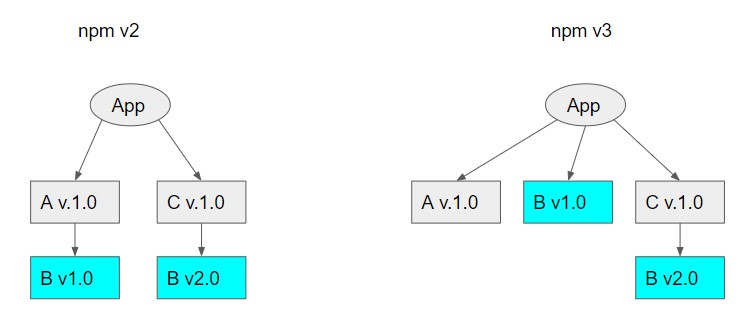
\includegraphics[width=.8\textwidth]{book/chapter-promisesandperils/pics/nestedv2.jpg}
	\caption{Difference between flat and nested dependencies}
	\label{fig:nest}
\end{figure}

\smallskip\noindent\textbf{Peril 5.}\textit{
Developers might declare a dependency to other parts of a software package ecosystem but not use it, e.g., because they failed to update its removal.
}\\

It is common for developers to declare dependencies on other parts of the software package ecosystem but not always use them. This can happen for various reasons, such as forgetting to remove the dependency after it is no longer needed. This can pose a challenge for researchers who are trying to extract dependencies from package managers, like those in configuration files, as there may be inconsistencies between the listed dependencies and what is actually being compiled and used by the code. This can lead to a biased understanding of the software package ecosystem and the relationships between software components.

To address this issue, there have been numerous efforts to track the actual library dependencies compiled and executed in software systems. These efforts aim to provide a more accurate understanding of the dependencies and the relationships between software components. For example, research has been conducted on the use of dynamic analysis to track compiled dependencies in real time and on the development of tools to automatically detect and track executed dependencies \cite{Zapata:ICSME2018, Ponta2018,Chinthanet:ASE2020}.

\subsection{Defining Boundaries and Completeness}

\smallskip\noindent\textbf{Promise 3.}\textit{
Researchers can use the boundaries of software package ecosystems to study communities of developers, e.g., developers contributing to and/or benefiting from the npm ecosystem.
}\\

Following Promise 2, the emergence of package managers has also led to studies that approximate software communities.
Using the libraries.io dataset, researchers were able to study projects that host libraries that use package managers.
Researchers have used this dataset to compare different library ecosystems \cite{kikas.2017,decan:emse:2019,CogoDown2019}.


\smallskip\noindent\textbf{Peril 6.}\textit{
Package managers do not always represent software package ecosystems, their communities, or their sub-communities, e.g., in cases where multiple package managers exist.
}\\

Package managers are a fundamental aspect of software package ecosystems, but do not always fully represent the complex relationships and interactions that occur within a community of developers and users, as shown in Table~\ref{tab:PM_features}. In some cases, multiple package managers exist for the same programming language, creating a complex landscape of software libraries and dependencies that are not always easily understood. For instance, Bower and Meteor manage npm libraries, which can lead to confusion and overlap in the management of dependencies.

Similarly, Java, Scala, Android, and other Java-based open source communities all use the Maven package manager, but each of these communities has its own unique set of libraries, dependencies, and development practises. Researchers should be aware of the limitations of package managers when studying software package ecosystems, and consider the broader context and relationships that exist within these communities. 

\smallskip\noindent\textbf{Peril 7.}\textit{
Lack of activity in parts of a software package ecosystem does not necessarily indicate project failure, e.g., when highly depended-upon libraries are feature-complete.
}\\

It is important to note that lack of activity in a part of a software package ecosystem does not always mean project failure \cite{coelho2017modern}. In some cases, highly relied-upon libraries that have reached feature-completeness may see little activity, but continue to be used by the software community. 

However, it is still important to consider the long-term sustainability of these libraries, especially given the rate at which technology and software development practises change. This has become a topic of interest in recent years, and researchers have explored best practises for sustaining open source projects and ensuring their continued success \cite{Ait2022,valiev2018ecosystem}. Understanding the factors that contribute to project sustainability is important to ensure the longevity and continued growth of software package ecosystems.

\smallskip\noindent\textbf{Peril 8.}\textit{
Sampling from a software package ecosystem is challenging since sub-setting might alter the dependency network, e.g., by breaking dependency chains.
}\\

Sampling from a package ecosystem is not straightforward, as the sample composition can be significantly affected due to missing dependency links between libraries. For instance, a subset of the ecosystem might alter the dependencies between libraries, leading to the breakdown of the dependency chains. This could lead to an incomplete picture of the software package ecosystem, leading to incorrect conclusions from a study. To minimise this risk, researchers should carefully consider the boundaries of their study and choose the appropriate sampling method based on the research questions and goals. For example, researchers could focus on popular, highly dependent, or risk-vulnerable aspects of the ecosystem as a starting point. 
For some ecosystems, the number of downloads, GitHub stars, and watchers are other aspects for the researcher to utilise.


\smallskip\noindent\textbf{Peril 9.}\textit{
Sampling from a software package ecosystem is challenging since the dependency network changes over time, e.g., when dependencies are added, removed, upgraded, or downgraded.
}\\

The dynamic nature of package ecosystems and the constant changes to their dependencies can impact the generalisability of the results. Therefore, it is important to also consider the time granularity of the analysis. For example, if the goal is to understand the evolution of dependencies over time, a finer time granularity may be necessary to capture the smaller changes and trends. However, if the goal is to understand the overall structure and relationships within the ecosystem, a coarser time granularity may be sufficient. Based on recent studies \cite{wattanakriengkrai2022giving,valiev2018ecosystem,Mirsaeedi:icse2020, Brindescu:emse2020, Nassif:icsme2017}, a three-month window seems appropriate for some studies.
Another level of granularity to consider is the size of the component. For instance, there are cases where a single package may contain more than one repository, especially for large library frameworks. 
The granularity also depends on the nature of the ecosystem itself. For instance, researchers should understand whether the ecosystem comprises library packages (e.g., PyPI), plugins (e.g., Eclipse), or is a library distribution (e.g., Android).



\subsection{Analysing and Visualising the Data}

\textbf{Peril 10.}\textit{
Analysing and visualising entire software package ecosystems is challenging due to their size, e.g., in terms of nodes and edges in the network.
}\\

The size of software package ecosystems implies large data sets, which can be overwhelming for tools and algorithms to analyse and display. Therefore, it may be necessary to make choices about the granularity of the data included in the analysis and visualisation. Another alternative is to focus on the most critical parts of the software package ecosystem, such as the high-level structure, highly dependent packages, or parts of the system that pose a risk to security and reliability. 
The key is to strike a balance between detail and simplicity, providing a meaningful representation of the ecosystem while being able to handle the complexity of its size.


\section{Application: When to Apply Which Peril}
\label{PPM:sec:application}

We include a disclaimer stating that not all perils are applicable to every mining situation. To demonstrate the practical application of our perils and their mitigation, we present two case studies that involve mining the software package ecosystem. Each case study has a distinct research objective and focusses on a specific dataset to be mined.

\subsection{Two Case Studies}
Table \ref{tab:cases} presents the two case studies we have selected for this analysis.
The \textit{first case} involves mining for contributions congruent to dependency updates \cite{wattanakriengkrai2022giving}. 
In this work, the authors mine GitHub repositories for Pull Requests and Issues that were submitted and merged congruent to dependency updates within the npm ecosystem. 
The \textit{second case} involves mining communication data for the Eclipse ecosystem \cite{Nugroho2021}. Although the second case does not mine for dependency relations (i.e., use relations),  we show that these perils still apply when mining for other relationships in an ecosystem.
Moreover, the second case studies the Eclipse ecosystem, which is a different dataset compared to the more popular GitHub dataset.

\subsection{Applying Perils and their Mitigation Strategies}
Table \ref{tab:perilsapp} provides a summary of the perils that can be applied to each of the case studies. We will now go into the details of mitigation strategies based on these perils. 
For better organisation and understanding, we have grouped the perils according to the four logical processes for mining.

\smallskip\noindent\textbf{Information to Mine}. 
The first set of mitigation strategies, which addresses perils 1-3, focusses on planning which information to mine. There are two primary strategies that researchers can employ:


\begin{enumerate}
    \item Researchers should use research tools and techniques to remove noise and other biases in the dataset, such as bot detection and the handling of multiple identities. This strategy was implemented in both case studies, as contributions and discussions often have the potential to involve bots or developers with multiple identities.
\item Depending on the research goals, researchers should recognise that not all contributions are equal and filter the dataset accordingly.
\end{enumerate}

We applied these two strategies to both cases. In the first case, the goal was to capture all congruent contributions, so we filtered out contributions made to libraries without dependencies. Since all npm packages are listed in the registry, Peril 3 (private activities) did not apply.
In the second case, we addressed Peril 1 by conducting a qualitative analysis to ensure that the member identities were not duplicated, as Eclipse developers were known to change identities. To mitigate Peril 2, we removed bot responses. For the second case, since all forum data is made public, Peril 3 did not apply.


\begin{table}
\centering
\caption{Description of the research objectives and datasets for the case studies}
 \label{tab:cases}
\begin{tabular}{lp{5cm}r} 
\toprule
\textbf{Case Study} & \textbf{Research Objective}                                                          & \textbf{Datasets}           \\
\midrule
Wattanakriengkrai \etal \cite{wattanakriengkrai2022giving}             & Explore code contributions between library and client (i.e, use-relations)  & libraries.io\\
& &  GitHub API \\
Nugroho \etal \cite{Nugroho2021}                & Explore discussion contributions between contributors (i.e., contributions) & Eclipse API                \\
\bottomrule
\end{tabular}
\end{table}

\begin{table}
\centering
\caption{Application of each peril to the case studies}
 \label{tab:perilsapp}
\begin{tabular}{rp{8cm}ccc} 
\toprule                   
& \textbf{Perils}       & case 1      & case 2                 \\
                                                                               & & npm  & Eclipse   \\
\midrule
\textbf{P1} &Developers might use different identifiers when contributing to different parts of a software package ecosystem, e.g., when contributing to different libraries.                             &    \CheckedBox         &          \CheckedBox           \\ 
%\hline
\textbf{P2} & Developers' contributions to software package ecosystems might be interspersed with bot contributions, e.g., automated dependency updates.                                                      &      \CheckedBox               &      \CheckedBox               \\ 
%\hline
\textbf{P3} & Not all developer activities in software package ecosystems are accessible to the public, e.g., library use in proprietary settings.                                                         &         -           &      \CheckedBox               \\ 
%\hline
\textbf{P4} & Different software package ecosystems define the concept of \`{}\`{}dependency'' differently, e.g., by allowing or not allowing different versions of a library on the same dependency tree. &         \CheckedBox       &     -                            \\ 
%\hline
\textbf{P5} & Developers might declare a dependency to other parts of a software package ecosystem but not use it, e.g., because they failed to update its removal.                                        &     -           &  -    \\
%\hline
\textbf{P6} &Package managers do not always represent software package ecosystems, their communities, or their sub-communities, e.g., in cases where multiple package managers exist.                     &     -                   &  -                  \\
%\hline
\textbf{P7} & Lack of activity in parts of a software package ecosystem does not necessarily indicate project failure, e.g., when highly depended-upon libraries are feature-complete.                     &       \CheckedBox         &  -                           \\
%\hline
\textbf{P8} &Sampling from a software package ecosystem is challenging since sub-setting might alter the dependency network, e.g., by breaking dependency chains.                                         &        \CheckedBox        &     \CheckedBox                                \\
%\hline
\textbf{P9} &Sampling from a software package ecosystem is challenging since the dependency network changes over time, e.g., when dependencies are added, removed, upgraded, or downgraded.               &       \CheckedBox         &     -                          \\
%\hline
\textbf{P10} &Analysing and visualising entire software package ecosystems is challenging due to their size, e.g., in terms of nodes and edges in the network.                                  &        \CheckedBox      &      \CheckedBox               \\
\bottomrule
\end{tabular}
\end{table}

\smallskip\noindent\textbf{Defining Dependencies}. 
The second set of perils (Perils 4-5) is related to dependency relationships between software units, and only the first case study is applicable. To address these perils, researchers should adopt the following strategy:

\begin{enumerate}
    \item Researchers should not rely solely on listed dependencies in configuration files (e.g., pom.xml, package.json, etc.) as a measure of dependency between two components. Instead, code-centric approaches should be used to validate which libraries are actually depended upon.
\end{enumerate}

For example, in the first case, in addition to mining the configuration information, the authors also analysed the similarity of the source code contributions to address Peril 4. Regarding Peril 5, since the study's objective was to investigate changes to the configuration files, the risk of the update not being executed was deemed less important.
It is important to note that the second case study did not include dependency analysis and, therefore, these perils did not apply.

\begin{figure*}[]
    \centering
    \begin{subfigure}{0.9\linewidth}
         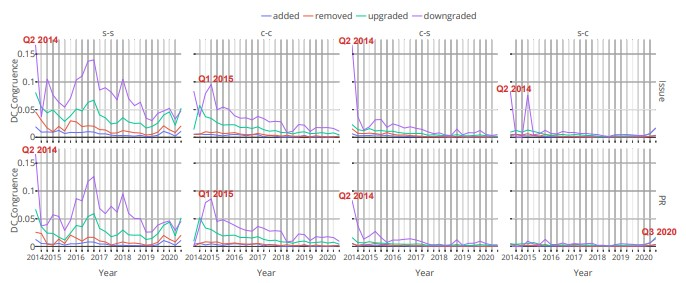
\includegraphics[width=1.1\textwidth]{book/chapter-promisesandperils/pics/congruentViz.jpg}
         \caption{Visualization of a Time analysis for 107,242 libraries.}
     \end{subfigure}
     \begin{subfigure}{0.9\linewidth}
         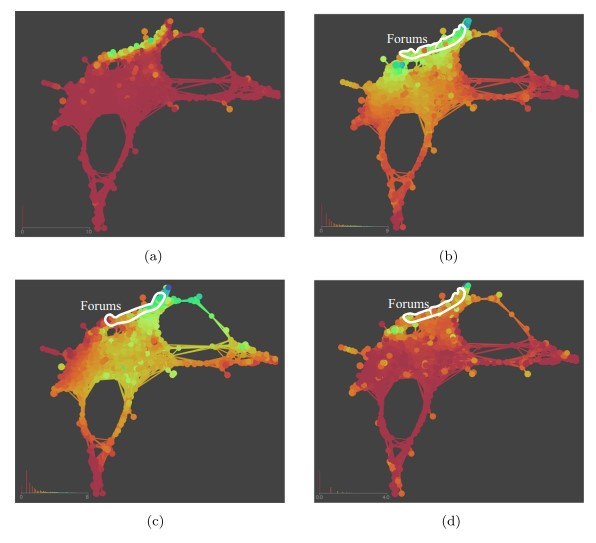
\includegraphics[width=1\textwidth]{book/chapter-promisesandperils/pics/eclipseViz.jpg}
         \caption{A Visual Topology map for 832,058 threads}
     \end{subfigure}
    \caption{Visualisation examples for the two case studies}
    \label{fig:visCase}
\end{figure*}

\smallskip\noindent\textbf{Defining Boundaries}.
The third set of perils (Perils 6-9) is related to the definition of boundaries and completeness and is relevant for both case studies. To mitigate these perils, we recommend the following strategies:

\begin{enumerate}
    \item Researchers should recognise that a dormant project does not necessarily mean that it is inactive. Instead, studies can use alternative heuristics, such as the number of dependents and dependencies, as better indicators of a project's importance in the ecosystem.
    \item Researchers should not rely solely on the programming language to define sub-communities. Using a common package manager for the programming language is a more effective rule of thumb for distinguishing boundaries.
    \item Researchers should avoid random sampling. Instead, sampling should be tailored to the research goals by considering factors such as an appropriate time window or focussing on specific attributes of components (e.g., most dependents, most popular, most contributors).
\end{enumerate}


Peril 6 did not apply to any of the case studies. 
Particularly for the first case, since the goal was to explore the npm package ecosystem, we assumed that the boundaries were clearly defined by the npm registry. 
Similarly, the second case study used the generic Eclipse platform as the boundary. 
Peril 7 was applied to the npm study, while Peril 8 was applied to both case studies. 
As a result, the two cases conducted a qualitative analysis of the dataset to gain deeper insights.
In the first case study, a three-month time window was created to capture dependencies. 
For the second case study, forum contributors were sampled into three groups (i.e., junior, member, or senior) according to the sliding window of their contributions. 

\smallskip\noindent\textbf{Visualisation}.
The final peril (Peril 10) relates to visualisation, which can be challenging due to the vast size and complexity of software ecosystems. As it is not feasible to visualise every aspect of an ecosystem simultaneously, a focused approach is necessary. A mitigation strategy is to select specific attributes of the ecosystem (e.g., the most dependent, most popular, and most contributions) that align with the research needs and objectives. 

Figure \ref{fig:visCase} shows two cases where visualizations are employed to gain insights, especially for large datasets.
In the first figure (a), we visualize the distributions of the data set and applied the appropriate statistical tests, along with the effect size, to test our hypotheses and answer research questions. 
In the second example (b), although not directly related to package ecosystems, the authors utilized a topological visualization \cite{Lum2013ExtractingIF} to gain insights on the over 800,000 forum threads of discussions. 



\section{Chapter Summary}
In this chapter, we explore the various aspects of mining information from the software package ecosystem, presenting three promises and ten perils that researchers should be aware of when undertaking such tasks. The chapter is structured around four key processes for mining: 1) Planning what Information to Mine, 2) Defining Components and their Dependencies, 3) Defining Boundaries and Completeness, and 4) Analysing and Visualising the Data. To help new and experienced researchers navigate these challenges, we introduced the SUG model, which can serve as a valuable tool to minimise threats to validity. Although some perils may be more relevant to specific research objectives, our aim is to equip researchers with the knowledge and resources needed to confidently gather and integrate software package ecosystem data into their work.
%The Software Heritage Research and Open Science Ecosystem
% %Semantic labeling three-letter-code: SWH (e.g. \chapter{SWH})


\title{Promises and Perils of Mining \\ Software Package Ecosystem Data}
\author{Raula Gaikovina Kula \and Katsuro Inoue \and Christoph Treude}
\institute{Raula Gaikovina Kula \at Nara Institute of Science and Technology, Japan, \email{raula-k@naist.jp}
\and Katsuro Inoue \at Nanzan University, Japan \email{ inoue599@nanzan-u.ac.jp}
\and  Christoph Treude \at The University of Melbourne, Australia \email{christoph.treude@unimelb.edu.au}}

\maketitle
\label{PPM:ch}
\abstract*{The use of third-party packages is becoming increasingly popular and has led to the emergence of large software package ecosystems with a maze of inter-dependencies. Since the reliance on these ecosystems enables developers to reduce development effort and increase productivity, it has attracted the interest of researchers: understanding the infrastructure and dynamics of package ecosystems has given rise to approaches for better code reuse, automated updates, and the avoidance of vulnerabilities, to name a few examples. But the reality of these ecosystems also poses challenges to software engineering researchers, such as: How do we obtain the complete network of dependencies along with the corresponding versioning information? What are the boundaries of these package ecosystem? How do we consistently detect dependencies that are declared but not used? How do we consistently identify developers within a package ecosystem? How much of the ecosystem do we need to understand to analyse a single component? How well do our approaches generalise across different programming languages and package ecosystems? In this chapter, we review promises and perils of mining the rich data related to software package ecosystems available to software engineering researchers.}

\abstract{The use of third-party packages is becoming increasingly popular and has led to the emergence of large software package ecosystems with a maze of inter-dependencies. Since the reliance on these ecosystems enables developers to reduce development effort and increase productivity, it has attracted the interest of researchers: understanding the infrastructure and dynamics of package ecosystems has given rise to approaches for better code reuse, automated updates, and the avoidance of vulnerabilities, to name a few examples. But the reality of these ecosystems also poses challenges to software engineering researchers, such as: How do we obtain the complete network of dependencies along with the corresponding versioning information? What are the boundaries of these package ecosystems? How do we consistently detect dependencies that are declared but not used? How do we consistently identify developers within a package ecosystem? How much of the ecosystem do we need to understand to analyse a single component? How well do our approaches generalise across different programming languages and package ecosystems? In this chapter, we review promises and perils of mining the rich data related to software package ecosystems available to software engineering researchers.}

%%%%%%%%%%%%%%%%%%%%%%%%%%%%%%%%%%%%%%%%%%%%%%%%%%%%%%%%%%%%%%%%%%

\section{Introduction}
\label{PPM:sec:definition}

Third-party libraries are a great way for developers to incorporate code without having to write their own for every functionality required. By using these libraries, developers can save time and energy while still getting the functions they need.
Using third-party libraries is becoming increasingly popular and has led to the emergence of large software package ecosystems such as npm. While these ecosystems offer many benefits, they also come with risks, such as software vulnerability attacks \cite{Chinthanet:ASE2020}.

Large software package ecosystems are a treasure trove for researchers who can investigate a wide range of questions. For example, by studying activity in large ecosystems, researchers can identify which libraries are the most popular and learn what characteristics make them successful \cite{kikas.2017,decan:emse:2019}.
Additionally, research on large ecosystems can help developers understand how to protect their code from malicious actors who may attempt to exploit vulnerabilities or insert malware into popular libraries.
Studying large software package ecosystems can help us better understand the dynamics of open source development in general. Open source development is a complex process that involves many different stakeholders working together (or sometimes competing) to create valuable code that anyone can use or improve upon. By understanding how these interactions play out in different types of ecosystem structures -- including those with many small projects versus few very large ones -- we can develop insights that might be applicable more broadly across other types of collaborative systems.

In this chapter, we identify and discuss promises and perils during the mining process, ranging from planning what information to mine from the ecosystem to analysing and visualising the mined data. 
Therefore, the chapter is broken down into these logical processes of mining ecosystem data: 1) Planning what Information to Mine, 2) Defining Components and their Dependencies, 3) Defining Boundaries and Completeness, and 4) Analysing and Visualising the Data.

This chapter is intended for researchers and practitioners who are interested in exploring and exploiting software package ecosystem information from a diverse range of sources that are publicly available. 
We also highlight the pitfalls to consider during the mining process, particularly when these pitfalls could lead to a misinterpretation of the analysis and results. 
The chapter is written in a manner that encourages newcomers who have little or no experience or who are interested in utilising ecosystem data across different disciplines outside of software engineering.
Our goal is to get new researchers quickly accustomed to gathering ecosystem information for their research.


\section{A Component-based Software Ecosystem}

Defined as a component-based software ecosystem, we suggest using the term `software package ecosystem' as a suitable term for the symbiotic relationships among third-party library components (as software projects or repositories), as these libraries and their dependent clients coexist on the same technological platform, therefore sharing the same environment and other internal and external factors (e.g., security threats, sharing contributions, etc.).
Please refer to the Introduction chapter for an in-depth definition of the different types of software ecosystems.
We present our interpretation of the software package ecosystem in Kula et al.~\cite{KulaSANER18}, where we formally define a package ecosystem using a Software Universe Graph (SUG).
This is modelled as a structured abstraction of the evolution of software systems and their library dependencies over time.

%%%%%%%%%%%%%%%%%%%%%%%%%%%%%%%%%%%%%%%%%%
\begin{figure*}
	\centering
	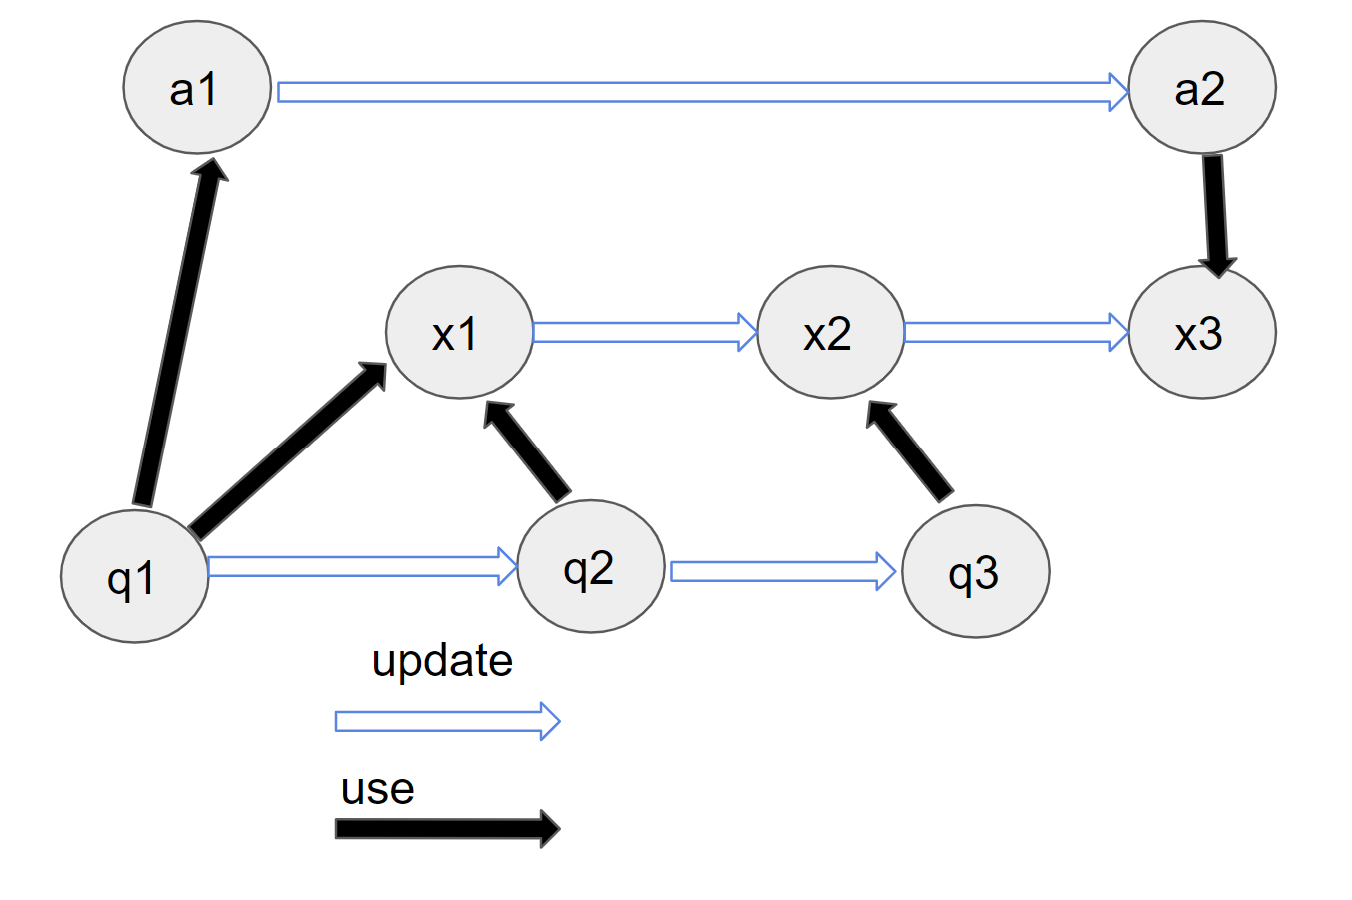
\includegraphics[width=.7\textwidth]{book/chapter-promisesandperils/pics/UniversalExample.jpg}
	\caption{Conceptual example of the Software Universe Graph, depicting the use and update relationships between different software units.}
	\label{fig:SUG}
\end{figure*}
%%%%%%%%%%%%%%%%%%%%%%%%%%%%%%%%%%%%%%%%%%%%%


\paragraph{\textbf{Component-based Representation as a Software Universe Graph}}
\label{PPM:sec:SUG}

First introduced by Kula et al.~\cite{KulaSANER18}, the \textit{Software Universe Graph} (SUG) is a structural abstraction of the software ecosystem of third-party libraries.
Figure \ref{fig:SUG} provides an illustration of the different relationships within the graph.
Let $G= (N,E)$ represent a graph $G$. $N$ is a set of nodes, each node representing a software unit. 
We define a software unit as a version instance of any software program. 

The authors then present the \textit{use} and \textit{update} relationships that exist in the ecosystem.
Hence, the edges $E$ are composed of $E_{use}$ and $E_{update}$. $E_{use}$ is a set of \textit{use-relations} and $E_{update}$ is a set of \textit{update-relations}.

\begin{definition}
An edge $u \rightarrow v \in E_{use}$ means that $u$ uses $v$. The defined functions of $E_{use}$ are:

\begin{equation}
\small
\small \use(u)\equiv \{v|u \rightarrow v\}
\normalsize
\end{equation}
\begin{equation}
\small
\small \useBy(u)\equiv \{v|v \rightarrow u\}
\normalsize
\end{equation}
\end{definition}

Use-relations can be extracted from either the source code or configuration files. 
As shown in Figure \ref{fig:SUG}, node $a1$ uses node $x1$. 
In addition, node $x1$ is used by nodes $a1$, $q1$, and $q2$. Parallel edges for node pairs are not allowed.

\begin{definition}
We represent an update relation from node $a$ to $b$ using $ a \Rightarrow b $, which means that the newer update $b$ was released from node $a$ and is defined as:
\begin{equation}
\small a \Rightarrow b \in E_{update}
\end{equation}
\end{definition}

Update relations refer to when a successive release of a software unit is made available. Figure \ref{fig:SUG} shows that node $q1$ is first updated to node $q2$. Later, node $q2$ is updated to the latest node $q3$. Hence, $q1 \Rightarrow q2 \Rightarrow q3$.
Note that an update should not be confused with forking. 
We distinguish a fork as a separate software unit. 
Each node in the SUG should be denoted by three attributes: \texttt{<name,release,time>}.  
For a node $u$, we define:

\begin{itemize}
	\item \textbf{u.name} Name is the string representation identifier of a software unit.
	We introduce the name axiom: For nodes $u$ and $v$, if $u \Rightarrow v$, then $u.name = v.name$ holds.
	
	\item \textbf{u.release}. Release refers to the specific assigned change reference for a software unit. For nodes $u$ and $v$, if $u \Rightarrow v$
	then $v$ is the immediate successor of $u$. Note that the versioning pattern may vary from project to project. 
	\item \textbf{u.time}. Time refers to the time stamp at which node $u$ was released. For nodes $u$ and $v$ of $u \Rightarrow v$, $u.time < v.time$.
\end{itemize}

\begin{figure}
	\centering
	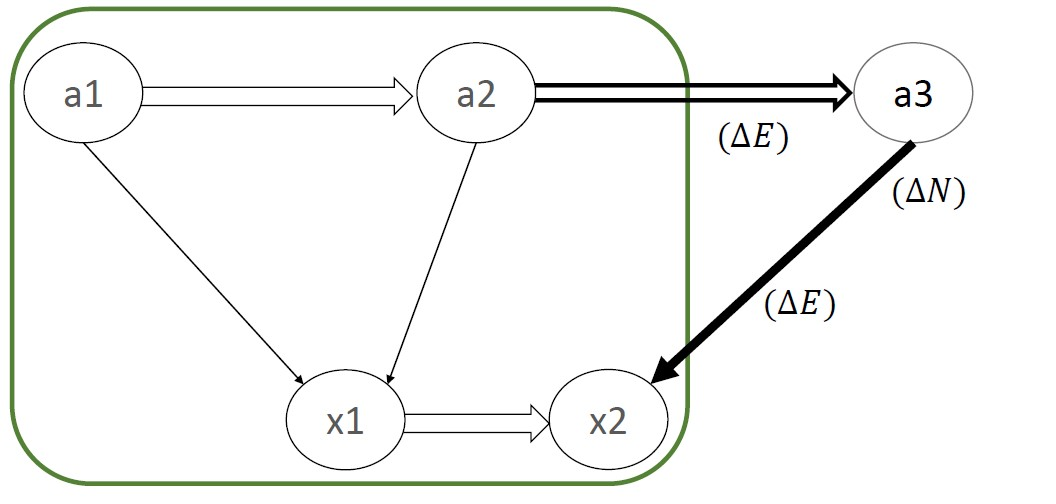
\includegraphics[width=.8\textwidth]{book/chapter-promisesandperils/pics/TemporalSUG.jpg}
	\caption{Temporal property of the SUG}
	\label{fig:SUGTemp}
\end{figure}

\begin{definition}
    
	The SUG has temporal properties.
This describes the simultaneity or ordering in reference to time. Let SUG $G = (N, E) $ be at time $t$. At time $t^{\prime} > t$, we observe an extension of $G$, such that:

\begin{equation}
\small G^{\prime} = (N \cup \Delta N, E \cup \Delta E)
\end{equation}
where $\Delta E \cap (N \times N) = \emptyset$
\end{definition}

Figure \ref{fig:SUGTemp} illustrates the temporal properties of the SUG. 
Here, it is observed that $G'$ is composed of $G$ augmented with newly added node $a3$ and its corresponding $a3 \rightarrow x2$ and $a2 \Rightarrow a3$ relations.
A SUG grows monotonically over time with only additions.
Here, we consider that modification or deletion changes on the SUG do not occur. 

\begin{definition}
    A timed SUG specifies the state of the SUG at any point in time.
So for an SUG $G=(N,E)$, we represent a timed SUG $G_{t}$ at time $t$ as a sub-graph of $G$. Formally,
\begin{equation}
\small G_t\equiv(N_{t}, E_{t})
\end{equation}
where $N_{t} = \{u|u \in N, u.time \leq t \}$ and $E_t = \{ e | e \in E \wedge e \in  N_t \}$
\end{definition}
	


\section{Data Sources}
Researchers can use various datasets to model the ecosystem using the SUG model of usage and update relationships.
The most obvious data source that has revolutionised data mining in the software engineering domain is the GitHub platform. 
Established in 2008, and then purchased by Microsoft in 2020, GitHub is home to various popular Open Source Software. 
GitHub is built on the git version control system and is useful for storing all changes made to a repository. 
In the case of the SUG, a GitHub repository can represent one software unit, whose depend relations can be extracted via a configuration file (such as the package.json file for JavaScript projects).
The repository should also contain the release information that holds the update relations.
Due to its large size, researchers and the GitHub team have made available datasets for researchers to mine, for example through the GitHub API/Graph QL.\footnote{\url{https://docs.github.com/en/graphql}} This is the backend Application Programming Interface (API) that can be used to query large amounts of data on GitHub. Most researchers use the API to download and mine information from the GitHub platform. 
It is important to note that while GitHub introduced a new feature of Dependency Graphs to map the depend relationship,\footnote{\url{https://docs.github.com/en/code-security/supply-chain-security/understanding-your-software-supply-chain/about-the-dependency-graph}} most older projects do not have this feature.
In this case, the researcher would need to manually extract and query the configuration files for dependency information. 

We refer to the first chapter for additional information on data sources for mining software ecosystems. 

\section{Promises and Perils}
\label{PPM:sec:promisesperils}

Using the SUG model of depend and use relations and the available datasets, we can now present our promises and perils of mining ecosystem information.

\subsection{Planning What Information to Mine}

\textbf{Promise 1.}\textit{
Researchers can access and link heterogeneous data related to software package ecosystems, e.g., package registries and bug trackers.}\\

When planning what information to mine from the ecosystem, researchers do not need to limit themselves to the usage and update relationship information.
Platforms that host software repositories include other software management systems such as bug trackers.
For example, GitHub allows researchers to manage GitHub Pull Requests, Issues, and Discussions not only for one project, but for multiple projects.
GitHub provides three management systems that are related to a software repository:

\begin{itemize}
    \item \textit{GitHub Discussions}\footnote{\url{https://docs.github.com/en/discussions}} - The GitHub Discussions forum is a collaborative communication forum for the community around an open source or internal project. Community members can ask and answer questions, share updates, have open-ended conversations, and follow along on decisions affecting the community's way of working.
    \item \textit{GitHub Pull Requests}\footnote{\url{https://docs.github.com/en/pull-requests}} - Pull Requests allow other developers from an ecosystem to make a contribution to a software repository. Pull requests also allow maintainers to discuss and review potential changes with collaborators and add follow-up commits before changes are merged into the software.
    \item \textit{GitHub Issues}\footnote{\url{https://docs.github.com/en/issues}} - Issues are used to track ideas, feedback, tasks, or bugs for work on GitHub.
\end{itemize}

These three systems are examples of how developers contribute to both their own and other projects. 
Hence, to incorporate this information, we can extend the SUG model, creating a model that includes a contribution relationship \cite{wattanakriengkrai2022giving}.

% Note that other platforms may also have management systems, like GitLab, BitBucket and Eclipse.

\begin{definition}
	A Dependency-Contribution graph incorporates contributions by developers whose libraries are involved in dependency relationships. 
\end{definition}

In this work \cite{wattanakriengkrai2022giving}, the authors explore the congruence between dependency updates and developer contributions, based on the original concept of social-technical congruence \cite{stcCataldo2008} where developers contribution patterns are congruent with their coordination needs. Hence, the goal is to identify contributions that are congruent to dependency updates.
As shown in Figure \ref{fig:lib} the authors extend from the typical SUG graph model where $lib_i$ depends (use) on  $lib_k$ and  $lib_j$, while  $lib_j$ also depends on $lib_k$, to the example shown in Figure \ref{fig:dc-graph}.
Different to the SUG, the graph captures developers and their contributions (i.e., the square as $dev_x$ and $dev_y$ represent two different developers making a contribution).
Here contributions are defined as $c$ (Pull Request or Issue) that were submitted to both a library and the client that depends on that library.
Hence, the graph can show contributions that are congruent to dependency changes for a software unit. 

\begin{figure}[t]
     \centering
     \begin{tikzpicture}[
         roundnode/.style={circle, fill=black, minimum size=5mm},
        squarenode/.style={fill=black, text=red, minimum size=5mm},
     ]
    \begin{scope}
         \node[roundnode, label=above:$lib_i$] (s2_proji) at (3, 2.5) {};
        \node[roundnode, label=below:$lib_j$] (s2_projj) at (4,0) {};
         \node[roundnode, label=below:$lib_k$] (s2_projk) at (2,0) {};
     \end{scope}

     \begin{scope} [every edge/.style={draw=gray, very thick}]
         \path [->] (s2_proji) edge (s2_projj);
         \path [->] (s2_proji) edge (s2_projk);
         \path [->] (s2_projj) edge (s2_projk);
     \end{scope}
     \end{tikzpicture}
    
     \caption{Example dependency graph for a given time period}
     \label{fig:lib}
     \vspace{2ex}
 \end{figure}
\begin{figure}[t]
    \centering

    \begin{tikzpicture}[
        roundnode/.style={circle, fill=black, minimum size=5mm},
        squarenode/.style={fill=black, text=red, minimum size=5mm},
    ]
    \begin{scope}
        
        \node[roundnode, label=right:$lib_i$] (s2_proji) at (4, 1.5) {};
        \node[roundnode, label=below:$lib_j$] (s2_projj) at (5,0) {};
        \node[roundnode, label=below:$lib_k$] (s2_projk) at (3,0) {};
        
        \node[squarenode, label=below:$dev_x$] (s3_devx) at (2, 3.5) {};
        
        \node[squarenode, label=below:$dev_y$] (s3_devy) at (6, 3.5) {};
        
    \end{scope}

    \begin{scope} [every edge/.style={draw=gray, very thick}]
        \path [->] (s2_proji)  edge  (s2_projj);
        \path [->] (s2_proji) edge (s2_projk);
        \path [->] (s2_projj) edge (s2_projk);
        
    \end{scope}
    \begin{scope} [every edge/.style={draw=gray, thick, double distance=2pt}]
        \path [->] (6, 2.8) edge node[left = 2mm] {$contribute$} (s2_proji);
        \path [->] (6, 2.8) edge[bend left=15] node[right = 1mm] {$contribute$} (s2_projj);
        \path [->] (2, 2.8) edge node[right = 2mm] {$$} (s2_proji);
        \path [->] (2, 2.8) edge[bend right=15] node[left = 1mm] {$contribute$} (s2_projk);
    \end{scope}
    \end{tikzpicture}
\end{figure}
\begin{figure}[t]
    \centering
    \begin{tikzpicture}[
        roundnode/.style={circle, fill=black, minimum size=5mm},
        squarenode/.style={fill=black, text=red, minimum size=5mm},
    ]
    \end{tikzpicture}
\caption{Example Dependency-Contribution graph showing relationships between contributions and dependencies}
 \label{fig:dc-graph}
\end{figure}

This is just one example of the type of research that is enabled by access to heterogeneous data related to software package ecosystems.

\smallskip\noindent\textbf{Peril 1.}\textit{
 Developers might use different identifiers when contributing to different parts of a software package ecosystem, e.g., when contributing to different libraries.}\\
 
When modelling using such graphs, there is a threat that contributors may use multiple identifiers (i.e., $c_x$ and $c_y$ are the same contributor).
This is a well-known research problem, and there has been work to merge these accounts, such as \cite{wiese2016mailing}.
GitHub has introduced mechanisms such as two-factor authentication\footnote{\url{https://docs.github.com/en/authentication/securing-your-account-with-two-factor-authentication-2fa/configuring-two-factor-authentication}} to counteract the issue of multiple identifiers.
This is since developers might be less likely to switch accounts if it requires cumbersome authentication.


\smallskip\noindent\textbf{Peril 2.}\textit{
Developers' contributions to software package ecosystems might be interspersed with bot contributions, e.g., automated dependency updates.}\\

The rise of automation and artificial intelligence has led to much work on the integration of automated scheduling (i.e., bots) into software development workflows \cite{Storey2016, Farooq2016, Wessel2018, Erlenhov2019, bot_modify_wf} to name a few. These bots are designed to perform specific tasks within a software package ecosystem. For example, a bot may be programmed to automatically update dependencies, test code changes, or deploy software to production. As an example, the Google APIs repo-automation-bots project lists bots for automated labelling of issues and pull requests, automated approval of pull requests, and triggering releases.\footnote{\url{https://github.com/googleapis/repo-automation-bots}}
Bots perform common maintenance tasks in many software projects and are now commonplace \cite{Beschastnikh2017, Urli2018,BIMAN,bot_or_not}.
Especially with bots such as dependabot (automated pull requests to update configurations to reduce the risk of vulnerability threats),\footnote{\url{https://github.com/dependabot}} more and more automation has caused a lot of noise in the contributions between projects.
There are also bots for communication and documentation \cite{Urli2018, Lin2016, Lebeuf2017a}.

To be able to draw accurate conclusions about what humans are doing in software package ecosystems, researchers should consider distinguishing between bot and human contributions.
It is also important to differentiate this from other contributions \cite{maeprasart2022understanding}.
The research community has responded well, with a wide range of techniques and tools to mitigate this peril \cite{Bodegha2021, golzadeh2022accuracy}.

\smallskip\noindent\textbf{Peril 3.}\textit{
Not all developer activities in software package ecosystems are accessible to the public, e.g., library use in proprietary settings.
}\\

Not all developer activities in software package ecosystems are accessible to the public, e.g., when the boundary between open source and industry is blurred \cite{stol2014inner}, which presents a challenge for researchers who aim to study the development process. This is particularly true in proprietary settings where software development is performed behind closed doors or is open source for a limited time period, thus resulting in the artefacts not permanently being publicly available.
This can make it difficult to understand the broader ecosystem in which a software project is developed.
Proprietary settings may lead to non-standardisation in software development practises. Different software projects may use different management systems and tools, making it difficult to accurately compare and analyse software development activities across various projects. For example, some projects may use communication, documentation, and other management tools not captured on the same platform \cite{montgomery2022alternative}. For example, some projects might use Bugzilla instead of issues and pull requests for their bug and code review systems, while others may use Discord, Slack channels, or email threads for their communication needs.

This lack of standardisation in software development practises presents a challenge for researchers who study the software package ecosystem and understand the development process. To address this issue, researchers should strive to collect data from a diverse set of projects to gain a comprehensive understanding of the software package ecosystem. In addition, researchers may need to adjust their methodologies or data collection techniques to accommodate the different tools and practises used by different software projects.

\subsection{Defining Components and their Dependencies}

\smallskip\noindent\textbf{Promise 2.}\textit{
Researchers can access a software package ecosystem's dependency network through package managers and registries, e.g., npm lists the dependencies and dependents for over a million libraries.}\\


With the rise of curated datasets like libraries.io, researchers can now recover and model dependency relations between software units using pre-extracted datasets.
Table \ref{tab:PM_features} shows examples of popular package managers mined from the libraries.io dataset in 2020. 

\begin{table*}[]
\caption{Summary of 13 package managers from libraries.io as ranked by TIOBE in 2020}
 \label{tab:PM_features}
 \centering
\begin{tabular}{@{}llrlll@{}}
\toprule
\begin{tabular}[c]{@{}l@{}}Package \\ Ecosystem\end{tabular} & \begin{tabular}[c]{@{}l@{}}Programming \\ Language\end{tabular} &  \begin{tabular}[c]{@{}l@{}}Tiobe \\ Rank\end{tabular} & Environment & \begin{tabular}[c]{@{}l@{}}Dependency \\ Tree\end{tabular} & \begin{tabular}[c]{@{}l@{}}Package   \\Archive link\end{tabular}\\ \midrule
PyPI & Python & 2 & Python & Flat & pypi.org  \\
Maven & Java & 3 & JVM & Flat & Maven.org  \\
Bower & JavaScript & 7 & Node.js & Flat & bower.io  \\
Meteor & JavaScript & 7 & Node.js & Nested & atmospherejs.com \\
npm & JavaScript & 7 & Node.js & Nested (v2) & npmjs.com  \\
Packagist & PHP & 8 & PHP & Flat & packagist.org \\
Puppet & Ruby & 13 & Ruby MRI & Flat & forge.puppet.com  \\
RubyGems & Ruby & 13 & Ruby MRI & Flat & rubygems.org  \\
CRAN & R & 14 & RStudio & Flat & cran.r-project.org  \\
CPAN & Perl & 15 & Perl & Flat & metacpan.org  \\
GO & Golang & 20 & Go & Flat & pkg.go.dev  \\
NuGet & C\#, VB & 5, 6 & .NET & Flat & nuget.org \\
Anaconda & Python, R, C\# & 2, 14, 5 & Anaconda & Flat & anaconda.org  \\ \bottomrule
\end{tabular}
\end{table*}

\smallskip\noindent\textbf{Peril 4.}\textit{
Different software package ecosystems define the concept of ``dependency'' differently, e.g., by allowing or not allowing different versions of a library on the same dependency tree.
}\\

Different software package ecosystems have varying definitions of what constitutes a dependency. For example, some ecosystems may allow multiple versions of a library to exist on the same dependency tree, while others may restrict developers to a single version of a library \cite{Islam}. These restrictions are often based on the programming language being used, as different languages have different approaches to managing dependencies. It is important to consider the restrictions on dependency relationships when studying software package ecosystems, as they can have a major impact on the development process. For example, the ability to use multiple versions of a library on the same dependency tree can greatly simplify the process of updating dependencies and can make it easier to resolve conflicts between libraries.

One way to visualise the impact of these restrictions is to compare the difference between a nested dependency tree and a directed dependency tree, as shown in Figure \ref{fig:nest}.\footnote{Taken from \url{https://npm.github.io/how-npm-works-docs/npm3/how-npm3-works.html}} This distinction is important because it highlights the different ways that a software unit can depend on different versions of the same library.
In this example, npm v3 creates the dependency tree based on the installation order, therefore flattening unnecessary nested dependencies (i.e., B v1.0 in cyan). This reduces the complexity of a nested tree by resolving some of the transitive dependencies (nested dependencies).

\begin{figure}
	\centering
	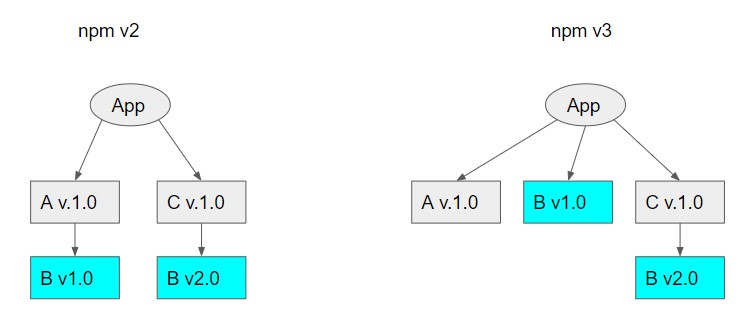
\includegraphics[width=.8\textwidth]{book/chapter-promisesandperils/pics/nestedv2.jpg}
	\caption{Difference between flat and nested dependencies}
	\label{fig:nest}
\end{figure}

\smallskip\noindent\textbf{Peril 5.}\textit{
Developers might declare a dependency to other parts of a software package ecosystem but not use it, e.g., because they failed to update its removal.
}\\

It is common for developers to declare dependencies on other parts of the software package ecosystem but not always use them. This can happen for various reasons, such as forgetting to remove the dependency after it is no longer needed. This can pose a challenge for researchers who are trying to extract dependencies from package managers, like those in configuration files, as there may be inconsistencies between the listed dependencies and what is actually being compiled and used by the code. This can lead to a biased understanding of the software package ecosystem and the relationships between software components.

To address this issue, there have been numerous efforts to track the actual library dependencies compiled and executed in software systems. These efforts aim to provide a more accurate understanding of the dependencies and the relationships between software components. For example, research has been conducted on the use of dynamic analysis to track compiled dependencies in real time and on the development of tools to automatically detect and track executed dependencies \cite{Zapata:ICSME2018, Ponta2018,Chinthanet:ASE2020}.

\subsection{Defining Boundaries and Completeness}

\smallskip\noindent\textbf{Promise 3.}\textit{
Researchers can use the boundaries of software package ecosystems to study communities of developers, e.g., developers contributing to and/or benefiting from the npm ecosystem.
}\\

Following Promise 2, the emergence of package managers has also led to studies that approximate software communities.
Using the libraries.io dataset, researchers were able to study projects that host libraries that use package managers.
Researchers have used this dataset to compare different library ecosystems \cite{kikas.2017,decan:emse:2019,CogoDown2019}.


\smallskip\noindent\textbf{Peril 6.}\textit{
Package managers do not always represent software package ecosystems, their communities, or their sub-communities, e.g., in cases where multiple package managers exist.
}\\

Package managers are a fundamental aspect of software package ecosystems, but do not always fully represent the complex relationships and interactions that occur within a community of developers and users, as shown in Table~\ref{tab:PM_features}. In some cases, multiple package managers exist for the same programming language, creating a complex landscape of software libraries and dependencies that are not always easily understood. For instance, Bower and Meteor manage npm libraries, which can lead to confusion and overlap in the management of dependencies.

Similarly, Java, Scala, Android, and other Java-based open source communities all use the Maven package manager, but each of these communities has its own unique set of libraries, dependencies, and development practises. Researchers should be aware of the limitations of package managers when studying software package ecosystems, and consider the broader context and relationships that exist within these communities. 

\smallskip\noindent\textbf{Peril 7.}\textit{
Lack of activity in parts of a software package ecosystem does not necessarily indicate project failure, e.g., when highly depended-upon libraries are feature-complete.
}\\

It is important to note that lack of activity in a part of a software package ecosystem does not always mean project failure \cite{coelho2017modern}. In some cases, highly relied-upon libraries that have reached feature-completeness may see little activity, but continue to be used by the software community. 

However, it is still important to consider the long-term sustainability of these libraries, especially given the rate at which technology and software development practises change. This has become a topic of interest in recent years, and researchers have explored best practises for sustaining open source projects and ensuring their continued success \cite{Ait2022,valiev2018ecosystem}. Understanding the factors that contribute to project sustainability is important to ensure the longevity and continued growth of software package ecosystems.

\smallskip\noindent\textbf{Peril 8.}\textit{
Sampling from a software package ecosystem is challenging since sub-setting might alter the dependency network, e.g., by breaking dependency chains.
}\\

Sampling from a package ecosystem is not straightforward, as the sample composition can be significantly affected due to missing dependency links between libraries. For instance, a subset of the ecosystem might alter the dependencies between libraries, leading to the breakdown of the dependency chains. This could lead to an incomplete picture of the software package ecosystem, leading to incorrect conclusions from a study. To minimise this risk, researchers should carefully consider the boundaries of their study and choose the appropriate sampling method based on the research questions and goals. For example, researchers could focus on popular, highly dependent, or risk-vulnerable aspects of the ecosystem as a starting point. 
For some ecosystems, the number of downloads, GitHub stars, and watchers are other aspects for the researcher to utilise.


\smallskip\noindent\textbf{Peril 9.}\textit{
Sampling from a software package ecosystem is challenging since the dependency network changes over time, e.g., when dependencies are added, removed, upgraded, or downgraded.
}\\

The dynamic nature of package ecosystems and the constant changes to their dependencies can impact the generalisability of the results. Therefore, it is important to also consider the time granularity of the analysis. For example, if the goal is to understand the evolution of dependencies over time, a finer time granularity may be necessary to capture the smaller changes and trends. However, if the goal is to understand the overall structure and relationships within the ecosystem, a coarser time granularity may be sufficient. Based on recent studies \cite{wattanakriengkrai2022giving,valiev2018ecosystem,Mirsaeedi:icse2020, Brindescu:emse2020, Nassif:icsme2017}, a three-month window seems appropriate for some studies.
Another level of granularity to consider is the size of the component. For instance, there are cases where a single package may contain more than one repository, especially for large library frameworks. 
The granularity also depends on the nature of the ecosystem itself. For instance, researchers should understand whether the ecosystem comprises library packages (e.g., PyPI), plugins (e.g., Eclipse), or is a library distribution (e.g., Android).



\subsection{Analysing and Visualising the Data}

\textbf{Peril 10.}\textit{
Analysing and visualising entire software package ecosystems is challenging due to their size, e.g., in terms of nodes and edges in the network.
}\\

The size of software package ecosystems implies large data sets, which can be overwhelming for tools and algorithms to analyse and display. Therefore, it may be necessary to make choices about the granularity of the data included in the analysis and visualisation. Another alternative is to focus on the most critical parts of the software package ecosystem, such as the high-level structure, highly dependent packages, or parts of the system that pose a risk to security and reliability. 
The key is to strike a balance between detail and simplicity, providing a meaningful representation of the ecosystem while being able to handle the complexity of its size.


\section{Application: When to Apply Which Peril}
\label{PPM:sec:application}

We include a disclaimer stating that not all perils are applicable to every mining situation. To demonstrate the practical application of our perils and their mitigation, we present two case studies that involve mining the software package ecosystem. Each case study has a distinct research objective and focusses on a specific dataset to be mined.

\subsection{Two Case Studies}
Table \ref{tab:cases} presents the two case studies we have selected for this analysis.
The \textit{first case} involves mining for contributions congruent to dependency updates \cite{wattanakriengkrai2022giving}. 
In this work, the authors mine GitHub repositories for Pull Requests and Issues that were submitted and merged congruent to dependency updates within the npm ecosystem. 
The \textit{second case} involves mining communication data for the Eclipse ecosystem \cite{Nugroho2021}. Although the second case does not mine for dependency relations (i.e., use relations),  we show that these perils still apply when mining for other relationships in an ecosystem.
Moreover, the second case studies the Eclipse ecosystem, which is a different dataset compared to the more popular GitHub dataset.

\subsection{Applying Perils and their Mitigation Strategies}
Table \ref{tab:perilsapp} provides a summary of the perils that can be applied to each of the case studies. We will now go into the details of mitigation strategies based on these perils. 
For better organisation and understanding, we have grouped the perils according to the four logical processes for mining.

\smallskip\noindent\textbf{Information to Mine}. 
The first set of mitigation strategies, which addresses perils 1-3, focusses on planning which information to mine. There are two primary strategies that researchers can employ:


\begin{enumerate}
    \item Researchers should use research tools and techniques to remove noise and other biases in the dataset, such as bot detection and the handling of multiple identities. This strategy was implemented in both case studies, as contributions and discussions often have the potential to involve bots or developers with multiple identities.
\item Depending on the research goals, researchers should recognise that not all contributions are equal and filter the dataset accordingly.
\end{enumerate}

We applied these two strategies to both cases. In the first case, the goal was to capture all congruent contributions, so we filtered out contributions made to libraries without dependencies. Since all npm packages are listed in the registry, Peril 3 (private activities) did not apply.
In the second case, we addressed Peril 1 by conducting a qualitative analysis to ensure that the member identities were not duplicated, as Eclipse developers were known to change identities. To mitigate Peril 2, we removed bot responses. For the second case, since all forum data is made public, Peril 3 did not apply.


\begin{table}
\centering
\caption{Description of the research objectives and datasets for the case studies}
 \label{tab:cases}
\begin{tabular}{lp{5cm}r} 
\toprule
\textbf{Case Study} & \textbf{Research Objective}                                                          & \textbf{Datasets}           \\
\midrule
Wattanakriengkrai \etal \cite{wattanakriengkrai2022giving}             & Explore code contributions between library and client (i.e, use-relations)  & libraries.io\\
& &  GitHub API \\
Nugroho \etal \cite{Nugroho2021}                & Explore discussion contributions between contributors (i.e., contributions) & Eclipse API                \\
\bottomrule
\end{tabular}
\end{table}

\begin{table}
\centering
\caption{Application of each peril to the case studies}
 \label{tab:perilsapp}
\begin{tabular}{rp{8cm}ccc} 
\toprule                   
& \textbf{Perils}       & case 1      & case 2                 \\
                                                                               & & npm  & Eclipse   \\
\midrule
\textbf{P1} &Developers might use different identifiers when contributing to different parts of a software package ecosystem, e.g., when contributing to different libraries.                             &    \CheckedBox         &          \CheckedBox           \\ 
%\hline
\textbf{P2} & Developers' contributions to software package ecosystems might be interspersed with bot contributions, e.g., automated dependency updates.                                                      &      \CheckedBox               &      \CheckedBox               \\ 
%\hline
\textbf{P3} & Not all developer activities in software package ecosystems are accessible to the public, e.g., library use in proprietary settings.                                                         &         -           &      \CheckedBox               \\ 
%\hline
\textbf{P4} & Different software package ecosystems define the concept of \`{}\`{}dependency'' differently, e.g., by allowing or not allowing different versions of a library on the same dependency tree. &         \CheckedBox       &     -                            \\ 
%\hline
\textbf{P5} & Developers might declare a dependency to other parts of a software package ecosystem but not use it, e.g., because they failed to update its removal.                                        &     -           &  -    \\
%\hline
\textbf{P6} &Package managers do not always represent software package ecosystems, their communities, or their sub-communities, e.g., in cases where multiple package managers exist.                     &     -                   &  -                  \\
%\hline
\textbf{P7} & Lack of activity in parts of a software package ecosystem does not necessarily indicate project failure, e.g., when highly depended-upon libraries are feature-complete.                     &       \CheckedBox         &  -                           \\
%\hline
\textbf{P8} &Sampling from a software package ecosystem is challenging since sub-setting might alter the dependency network, e.g., by breaking dependency chains.                                         &        \CheckedBox        &     \CheckedBox                                \\
%\hline
\textbf{P9} &Sampling from a software package ecosystem is challenging since the dependency network changes over time, e.g., when dependencies are added, removed, upgraded, or downgraded.               &       \CheckedBox         &     -                          \\
%\hline
\textbf{P10} &Analysing and visualising entire software package ecosystems is challenging due to their size, e.g., in terms of nodes and edges in the network.                                  &        \CheckedBox      &      \CheckedBox               \\
\bottomrule
\end{tabular}
\end{table}

\smallskip\noindent\textbf{Defining Dependencies}. 
The second set of perils (Perils 4-5) is related to dependency relationships between software units, and only the first case study is applicable. To address these perils, researchers should adopt the following strategy:

\begin{enumerate}
    \item Researchers should not rely solely on listed dependencies in configuration files (e.g., pom.xml, package.json, etc.) as a measure of dependency between two components. Instead, code-centric approaches should be used to validate which libraries are actually depended upon.
\end{enumerate}

For example, in the first case, in addition to mining the configuration information, the authors also analysed the similarity of the source code contributions to address Peril 4. Regarding Peril 5, since the study's objective was to investigate changes to the configuration files, the risk of the update not being executed was deemed less important.
It is important to note that the second case study did not include dependency analysis and, therefore, these perils did not apply.

\begin{figure*}[]
    \centering
    \begin{subfigure}{0.9\linewidth}
         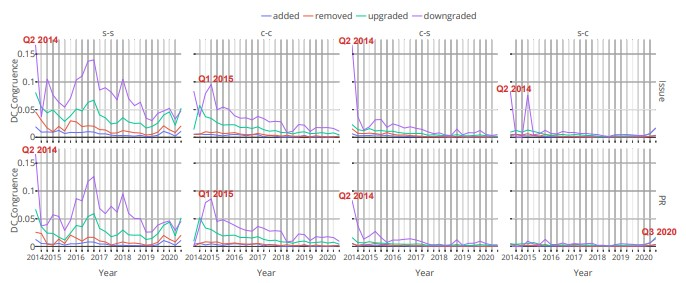
\includegraphics[width=1.1\textwidth]{book/chapter-promisesandperils/pics/congruentViz.jpg}
         \caption{Visualization of a Time analysis for 107,242 libraries.}
     \end{subfigure}
     \begin{subfigure}{0.9\linewidth}
         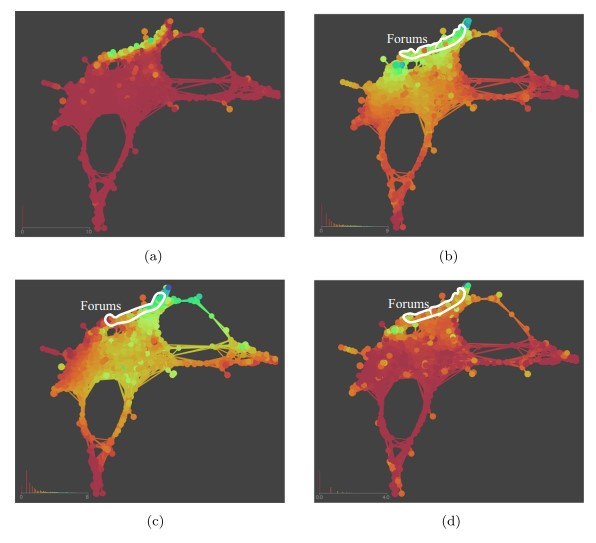
\includegraphics[width=1\textwidth]{book/chapter-promisesandperils/pics/eclipseViz.jpg}
         \caption{A Visual Topology map for 832,058 threads}
     \end{subfigure}
    \caption{Visualisation examples for the two case studies}
    \label{fig:visCase}
\end{figure*}

\smallskip\noindent\textbf{Defining Boundaries}.
The third set of perils (Perils 6-9) is related to the definition of boundaries and completeness and is relevant for both case studies. To mitigate these perils, we recommend the following strategies:

\begin{enumerate}
    \item Researchers should recognise that a dormant project does not necessarily mean that it is inactive. Instead, studies can use alternative heuristics, such as the number of dependents and dependencies, as better indicators of a project's importance in the ecosystem.
    \item Researchers should not rely solely on the programming language to define sub-communities. Using a common package manager for the programming language is a more effective rule of thumb for distinguishing boundaries.
    \item Researchers should avoid random sampling. Instead, sampling should be tailored to the research goals by considering factors such as an appropriate time window or focussing on specific attributes of components (e.g., most dependents, most popular, most contributors).
\end{enumerate}


Peril 6 did not apply to any of the case studies. 
Particularly for the first case, since the goal was to explore the npm package ecosystem, we assumed that the boundaries were clearly defined by the npm registry. 
Similarly, the second case study used the generic Eclipse platform as the boundary. 
Peril 7 was applied to the npm study, while Peril 8 was applied to both case studies. 
As a result, the two cases conducted a qualitative analysis of the dataset to gain deeper insights.
In the first case study, a three-month time window was created to capture dependencies. 
For the second case study, forum contributors were sampled into three groups (i.e., junior, member, or senior) according to the sliding window of their contributions. 

\smallskip\noindent\textbf{Visualisation}.
The final peril (Peril 10) relates to visualisation, which can be challenging due to the vast size and complexity of software ecosystems. As it is not feasible to visualise every aspect of an ecosystem simultaneously, a focused approach is necessary. A mitigation strategy is to select specific attributes of the ecosystem (e.g., the most dependent, most popular, and most contributions) that align with the research needs and objectives. 

Figure \ref{fig:visCase} shows two cases where visualizations are employed to gain insights, especially for large datasets.
In the first figure (a), we visualize the distributions of the data set and applied the appropriate statistical tests, along with the effect size, to test our hypotheses and answer research questions. 
In the second example (b), although not directly related to package ecosystems, the authors utilized a topological visualization \cite{Lum2013ExtractingIF} to gain insights on the over 800,000 forum threads of discussions. 



\section{Chapter Summary}
In this chapter, we explore the various aspects of mining information from the software package ecosystem, presenting three promises and ten perils that researchers should be aware of when undertaking such tasks. The chapter is structured around four key processes for mining: 1) Planning what Information to Mine, 2) Defining Components and their Dependencies, 3) Defining Boundaries and Completeness, and 4) Analysing and Visualising the Data. To help new and experienced researchers navigate these challenges, we introduced the SUG model, which can serve as a valuable tool to minimise threats to validity. Although some perils may be more relevant to specific research objectives, our aim is to equip researchers with the knowledge and resources needed to confidently gather and integrate software package ecosystem data into their work.
%Promises and Perils of Mining Software Ecosystem Data
%Semantic labeling three-letter-code: PPM (e.g. \chapter{PPM})

% %%%%%%%%%%%%%%%%%%%%%part.tex%%%%%%%%%%%%%%%%%%%%%%%%%%%%%%%%%%
% 
% sample part title
%
% Use this file as a template for your own input.
%
%%%%%%%%%%%%%%%%%%%%%%%% Springer %%%%%%%%%%%%%%%%%%%%%%%%%%

\begin{partbacktext}
\part{ANALYSING SOFTWARE ECOSYSTEMS}
\label{part:analysing}

\end{partbacktext} %ANALYSING SOFTWARE ECOSYSTEMS



% 
\title{Promises and Perils of Mining \\ Software Package Ecosystem Data}
\author{Raula Gaikovina Kula \and Katsuro Inoue \and Christoph Treude}
\institute{Raula Gaikovina Kula \at Nara Institute of Science and Technology, Japan, \email{raula-k@naist.jp}
\and Katsuro Inoue \at Nanzan University, Japan \email{ inoue599@nanzan-u.ac.jp}
\and  Christoph Treude \at The University of Melbourne, Australia \email{christoph.treude@unimelb.edu.au}}

\maketitle
\label{PPM:ch}
\abstract*{The use of third-party packages is becoming increasingly popular and has led to the emergence of large software package ecosystems with a maze of inter-dependencies. Since the reliance on these ecosystems enables developers to reduce development effort and increase productivity, it has attracted the interest of researchers: understanding the infrastructure and dynamics of package ecosystems has given rise to approaches for better code reuse, automated updates, and the avoidance of vulnerabilities, to name a few examples. But the reality of these ecosystems also poses challenges to software engineering researchers, such as: How do we obtain the complete network of dependencies along with the corresponding versioning information? What are the boundaries of these package ecosystem? How do we consistently detect dependencies that are declared but not used? How do we consistently identify developers within a package ecosystem? How much of the ecosystem do we need to understand to analyse a single component? How well do our approaches generalise across different programming languages and package ecosystems? In this chapter, we review promises and perils of mining the rich data related to software package ecosystems available to software engineering researchers.}

\abstract{The use of third-party packages is becoming increasingly popular and has led to the emergence of large software package ecosystems with a maze of inter-dependencies. Since the reliance on these ecosystems enables developers to reduce development effort and increase productivity, it has attracted the interest of researchers: understanding the infrastructure and dynamics of package ecosystems has given rise to approaches for better code reuse, automated updates, and the avoidance of vulnerabilities, to name a few examples. But the reality of these ecosystems also poses challenges to software engineering researchers, such as: How do we obtain the complete network of dependencies along with the corresponding versioning information? What are the boundaries of these package ecosystems? How do we consistently detect dependencies that are declared but not used? How do we consistently identify developers within a package ecosystem? How much of the ecosystem do we need to understand to analyse a single component? How well do our approaches generalise across different programming languages and package ecosystems? In this chapter, we review promises and perils of mining the rich data related to software package ecosystems available to software engineering researchers.}

%%%%%%%%%%%%%%%%%%%%%%%%%%%%%%%%%%%%%%%%%%%%%%%%%%%%%%%%%%%%%%%%%%

\section{Introduction}
\label{PPM:sec:definition}

Third-party libraries are a great way for developers to incorporate code without having to write their own for every functionality required. By using these libraries, developers can save time and energy while still getting the functions they need.
Using third-party libraries is becoming increasingly popular and has led to the emergence of large software package ecosystems such as npm. While these ecosystems offer many benefits, they also come with risks, such as software vulnerability attacks \cite{Chinthanet:ASE2020}.

Large software package ecosystems are a treasure trove for researchers who can investigate a wide range of questions. For example, by studying activity in large ecosystems, researchers can identify which libraries are the most popular and learn what characteristics make them successful \cite{kikas.2017,decan:emse:2019}.
Additionally, research on large ecosystems can help developers understand how to protect their code from malicious actors who may attempt to exploit vulnerabilities or insert malware into popular libraries.
Studying large software package ecosystems can help us better understand the dynamics of open source development in general. Open source development is a complex process that involves many different stakeholders working together (or sometimes competing) to create valuable code that anyone can use or improve upon. By understanding how these interactions play out in different types of ecosystem structures -- including those with many small projects versus few very large ones -- we can develop insights that might be applicable more broadly across other types of collaborative systems.

In this chapter, we identify and discuss promises and perils during the mining process, ranging from planning what information to mine from the ecosystem to analysing and visualising the mined data. 
Therefore, the chapter is broken down into these logical processes of mining ecosystem data: 1) Planning what Information to Mine, 2) Defining Components and their Dependencies, 3) Defining Boundaries and Completeness, and 4) Analysing and Visualising the Data.

This chapter is intended for researchers and practitioners who are interested in exploring and exploiting software package ecosystem information from a diverse range of sources that are publicly available. 
We also highlight the pitfalls to consider during the mining process, particularly when these pitfalls could lead to a misinterpretation of the analysis and results. 
The chapter is written in a manner that encourages newcomers who have little or no experience or who are interested in utilising ecosystem data across different disciplines outside of software engineering.
Our goal is to get new researchers quickly accustomed to gathering ecosystem information for their research.


\section{A Component-based Software Ecosystem}

Defined as a component-based software ecosystem, we suggest using the term `software package ecosystem' as a suitable term for the symbiotic relationships among third-party library components (as software projects or repositories), as these libraries and their dependent clients coexist on the same technological platform, therefore sharing the same environment and other internal and external factors (e.g., security threats, sharing contributions, etc.).
Please refer to the Introduction chapter for an in-depth definition of the different types of software ecosystems.
We present our interpretation of the software package ecosystem in Kula et al.~\cite{KulaSANER18}, where we formally define a package ecosystem using a Software Universe Graph (SUG).
This is modelled as a structured abstraction of the evolution of software systems and their library dependencies over time.

%%%%%%%%%%%%%%%%%%%%%%%%%%%%%%%%%%%%%%%%%%
\begin{figure*}
	\centering
	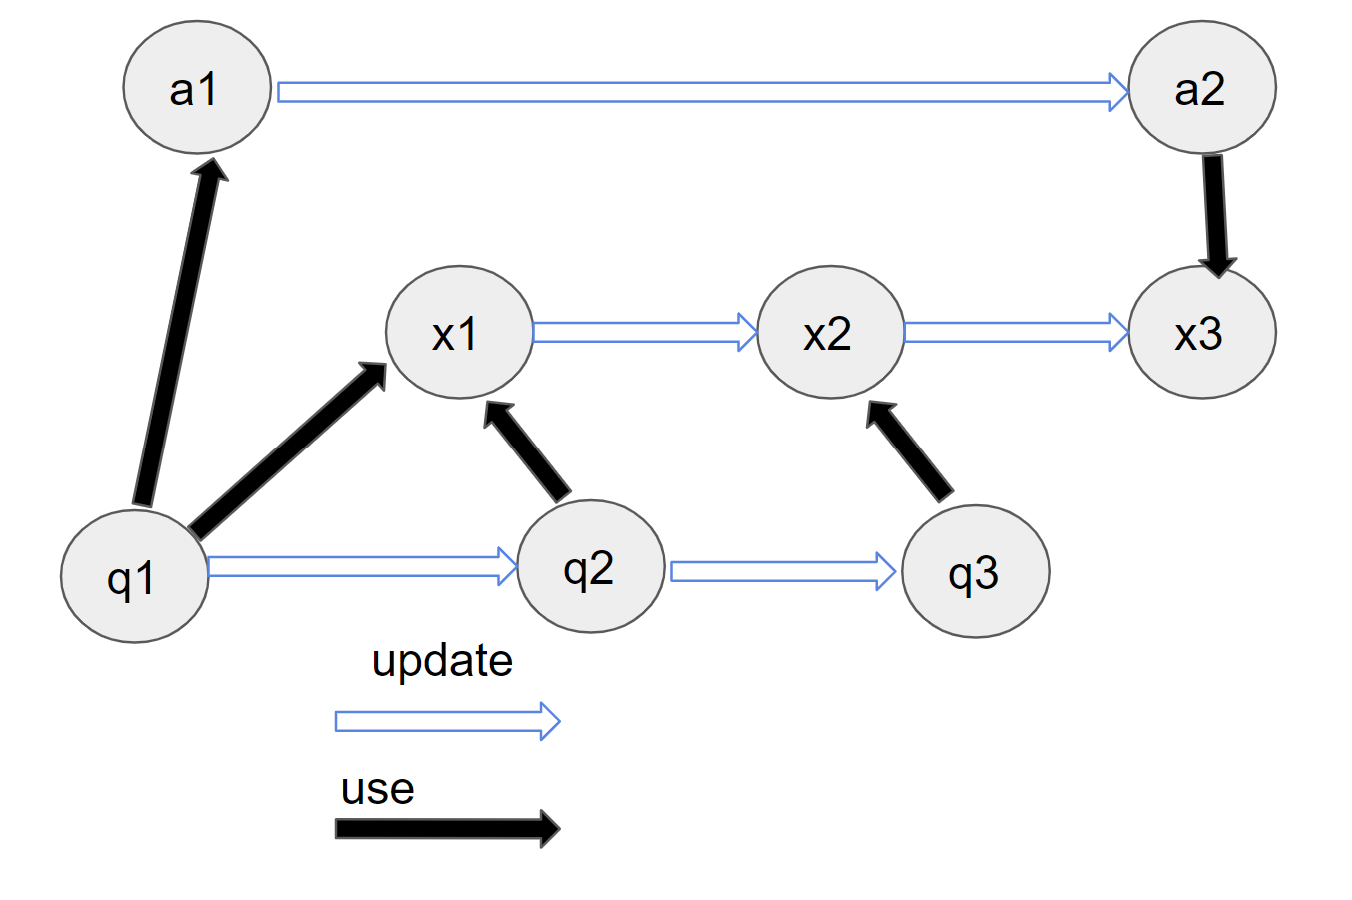
\includegraphics[width=.7\textwidth]{book/chapter-promisesandperils/pics/UniversalExample.jpg}
	\caption{Conceptual example of the Software Universe Graph, depicting the use and update relationships between different software units.}
	\label{fig:SUG}
\end{figure*}
%%%%%%%%%%%%%%%%%%%%%%%%%%%%%%%%%%%%%%%%%%%%%


\paragraph{\textbf{Component-based Representation as a Software Universe Graph}}
\label{PPM:sec:SUG}

First introduced by Kula et al.~\cite{KulaSANER18}, the \textit{Software Universe Graph} (SUG) is a structural abstraction of the software ecosystem of third-party libraries.
Figure \ref{fig:SUG} provides an illustration of the different relationships within the graph.
Let $G= (N,E)$ represent a graph $G$. $N$ is a set of nodes, each node representing a software unit. 
We define a software unit as a version instance of any software program. 

The authors then present the \textit{use} and \textit{update} relationships that exist in the ecosystem.
Hence, the edges $E$ are composed of $E_{use}$ and $E_{update}$. $E_{use}$ is a set of \textit{use-relations} and $E_{update}$ is a set of \textit{update-relations}.

\begin{definition}
An edge $u \rightarrow v \in E_{use}$ means that $u$ uses $v$. The defined functions of $E_{use}$ are:

\begin{equation}
\small
\small \use(u)\equiv \{v|u \rightarrow v\}
\normalsize
\end{equation}
\begin{equation}
\small
\small \useBy(u)\equiv \{v|v \rightarrow u\}
\normalsize
\end{equation}
\end{definition}

Use-relations can be extracted from either the source code or configuration files. 
As shown in Figure \ref{fig:SUG}, node $a1$ uses node $x1$. 
In addition, node $x1$ is used by nodes $a1$, $q1$, and $q2$. Parallel edges for node pairs are not allowed.

\begin{definition}
We represent an update relation from node $a$ to $b$ using $ a \Rightarrow b $, which means that the newer update $b$ was released from node $a$ and is defined as:
\begin{equation}
\small a \Rightarrow b \in E_{update}
\end{equation}
\end{definition}

Update relations refer to when a successive release of a software unit is made available. Figure \ref{fig:SUG} shows that node $q1$ is first updated to node $q2$. Later, node $q2$ is updated to the latest node $q3$. Hence, $q1 \Rightarrow q2 \Rightarrow q3$.
Note that an update should not be confused with forking. 
We distinguish a fork as a separate software unit. 
Each node in the SUG should be denoted by three attributes: \texttt{<name,release,time>}.  
For a node $u$, we define:

\begin{itemize}
	\item \textbf{u.name} Name is the string representation identifier of a software unit.
	We introduce the name axiom: For nodes $u$ and $v$, if $u \Rightarrow v$, then $u.name = v.name$ holds.
	
	\item \textbf{u.release}. Release refers to the specific assigned change reference for a software unit. For nodes $u$ and $v$, if $u \Rightarrow v$
	then $v$ is the immediate successor of $u$. Note that the versioning pattern may vary from project to project. 
	\item \textbf{u.time}. Time refers to the time stamp at which node $u$ was released. For nodes $u$ and $v$ of $u \Rightarrow v$, $u.time < v.time$.
\end{itemize}

\begin{figure}
	\centering
	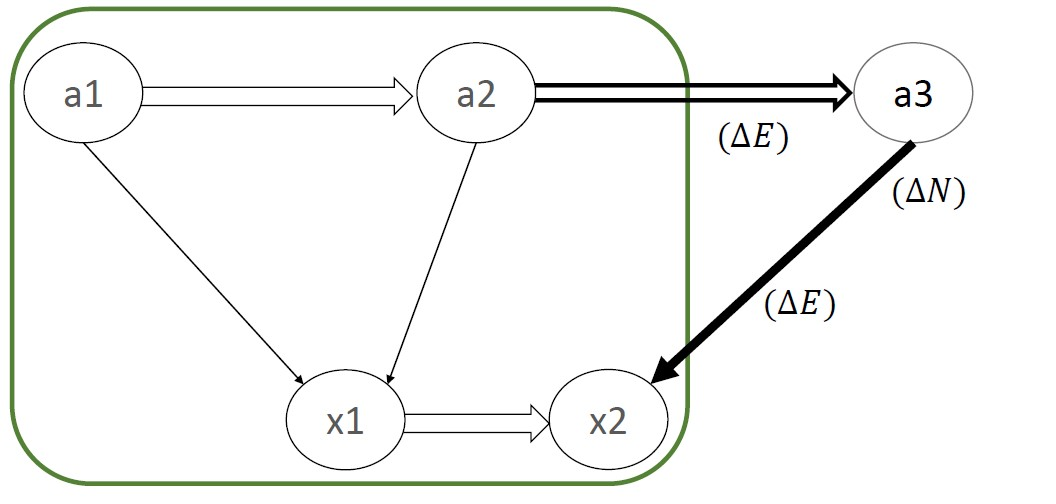
\includegraphics[width=.8\textwidth]{book/chapter-promisesandperils/pics/TemporalSUG.jpg}
	\caption{Temporal property of the SUG}
	\label{fig:SUGTemp}
\end{figure}

\begin{definition}
    
	The SUG has temporal properties.
This describes the simultaneity or ordering in reference to time. Let SUG $G = (N, E) $ be at time $t$. At time $t^{\prime} > t$, we observe an extension of $G$, such that:

\begin{equation}
\small G^{\prime} = (N \cup \Delta N, E \cup \Delta E)
\end{equation}
where $\Delta E \cap (N \times N) = \emptyset$
\end{definition}

Figure \ref{fig:SUGTemp} illustrates the temporal properties of the SUG. 
Here, it is observed that $G'$ is composed of $G$ augmented with newly added node $a3$ and its corresponding $a3 \rightarrow x2$ and $a2 \Rightarrow a3$ relations.
A SUG grows monotonically over time with only additions.
Here, we consider that modification or deletion changes on the SUG do not occur. 

\begin{definition}
    A timed SUG specifies the state of the SUG at any point in time.
So for an SUG $G=(N,E)$, we represent a timed SUG $G_{t}$ at time $t$ as a sub-graph of $G$. Formally,
\begin{equation}
\small G_t\equiv(N_{t}, E_{t})
\end{equation}
where $N_{t} = \{u|u \in N, u.time \leq t \}$ and $E_t = \{ e | e \in E \wedge e \in  N_t \}$
\end{definition}
	


\section{Data Sources}
Researchers can use various datasets to model the ecosystem using the SUG model of usage and update relationships.
The most obvious data source that has revolutionised data mining in the software engineering domain is the GitHub platform. 
Established in 2008, and then purchased by Microsoft in 2020, GitHub is home to various popular Open Source Software. 
GitHub is built on the git version control system and is useful for storing all changes made to a repository. 
In the case of the SUG, a GitHub repository can represent one software unit, whose depend relations can be extracted via a configuration file (such as the package.json file for JavaScript projects).
The repository should also contain the release information that holds the update relations.
Due to its large size, researchers and the GitHub team have made available datasets for researchers to mine, for example through the GitHub API/Graph QL.\footnote{\url{https://docs.github.com/en/graphql}} This is the backend Application Programming Interface (API) that can be used to query large amounts of data on GitHub. Most researchers use the API to download and mine information from the GitHub platform. 
It is important to note that while GitHub introduced a new feature of Dependency Graphs to map the depend relationship,\footnote{\url{https://docs.github.com/en/code-security/supply-chain-security/understanding-your-software-supply-chain/about-the-dependency-graph}} most older projects do not have this feature.
In this case, the researcher would need to manually extract and query the configuration files for dependency information. 

We refer to the first chapter for additional information on data sources for mining software ecosystems. 

\section{Promises and Perils}
\label{PPM:sec:promisesperils}

Using the SUG model of depend and use relations and the available datasets, we can now present our promises and perils of mining ecosystem information.

\subsection{Planning What Information to Mine}

\textbf{Promise 1.}\textit{
Researchers can access and link heterogeneous data related to software package ecosystems, e.g., package registries and bug trackers.}\\

When planning what information to mine from the ecosystem, researchers do not need to limit themselves to the usage and update relationship information.
Platforms that host software repositories include other software management systems such as bug trackers.
For example, GitHub allows researchers to manage GitHub Pull Requests, Issues, and Discussions not only for one project, but for multiple projects.
GitHub provides three management systems that are related to a software repository:

\begin{itemize}
    \item \textit{GitHub Discussions}\footnote{\url{https://docs.github.com/en/discussions}} - The GitHub Discussions forum is a collaborative communication forum for the community around an open source or internal project. Community members can ask and answer questions, share updates, have open-ended conversations, and follow along on decisions affecting the community's way of working.
    \item \textit{GitHub Pull Requests}\footnote{\url{https://docs.github.com/en/pull-requests}} - Pull Requests allow other developers from an ecosystem to make a contribution to a software repository. Pull requests also allow maintainers to discuss and review potential changes with collaborators and add follow-up commits before changes are merged into the software.
    \item \textit{GitHub Issues}\footnote{\url{https://docs.github.com/en/issues}} - Issues are used to track ideas, feedback, tasks, or bugs for work on GitHub.
\end{itemize}

These three systems are examples of how developers contribute to both their own and other projects. 
Hence, to incorporate this information, we can extend the SUG model, creating a model that includes a contribution relationship \cite{wattanakriengkrai2022giving}.

% Note that other platforms may also have management systems, like GitLab, BitBucket and Eclipse.

\begin{definition}
	A Dependency-Contribution graph incorporates contributions by developers whose libraries are involved in dependency relationships. 
\end{definition}

In this work \cite{wattanakriengkrai2022giving}, the authors explore the congruence between dependency updates and developer contributions, based on the original concept of social-technical congruence \cite{stcCataldo2008} where developers contribution patterns are congruent with their coordination needs. Hence, the goal is to identify contributions that are congruent to dependency updates.
As shown in Figure \ref{fig:lib} the authors extend from the typical SUG graph model where $lib_i$ depends (use) on  $lib_k$ and  $lib_j$, while  $lib_j$ also depends on $lib_k$, to the example shown in Figure \ref{fig:dc-graph}.
Different to the SUG, the graph captures developers and their contributions (i.e., the square as $dev_x$ and $dev_y$ represent two different developers making a contribution).
Here contributions are defined as $c$ (Pull Request or Issue) that were submitted to both a library and the client that depends on that library.
Hence, the graph can show contributions that are congruent to dependency changes for a software unit. 

\begin{figure}[t]
     \centering
     \begin{tikzpicture}[
         roundnode/.style={circle, fill=black, minimum size=5mm},
        squarenode/.style={fill=black, text=red, minimum size=5mm},
     ]
    \begin{scope}
         \node[roundnode, label=above:$lib_i$] (s2_proji) at (3, 2.5) {};
        \node[roundnode, label=below:$lib_j$] (s2_projj) at (4,0) {};
         \node[roundnode, label=below:$lib_k$] (s2_projk) at (2,0) {};
     \end{scope}

     \begin{scope} [every edge/.style={draw=gray, very thick}]
         \path [->] (s2_proji) edge (s2_projj);
         \path [->] (s2_proji) edge (s2_projk);
         \path [->] (s2_projj) edge (s2_projk);
     \end{scope}
     \end{tikzpicture}
    
     \caption{Example dependency graph for a given time period}
     \label{fig:lib}
     \vspace{2ex}
 \end{figure}
\begin{figure}[t]
    \centering

    \begin{tikzpicture}[
        roundnode/.style={circle, fill=black, minimum size=5mm},
        squarenode/.style={fill=black, text=red, minimum size=5mm},
    ]
    \begin{scope}
        
        \node[roundnode, label=right:$lib_i$] (s2_proji) at (4, 1.5) {};
        \node[roundnode, label=below:$lib_j$] (s2_projj) at (5,0) {};
        \node[roundnode, label=below:$lib_k$] (s2_projk) at (3,0) {};
        
        \node[squarenode, label=below:$dev_x$] (s3_devx) at (2, 3.5) {};
        
        \node[squarenode, label=below:$dev_y$] (s3_devy) at (6, 3.5) {};
        
    \end{scope}

    \begin{scope} [every edge/.style={draw=gray, very thick}]
        \path [->] (s2_proji)  edge  (s2_projj);
        \path [->] (s2_proji) edge (s2_projk);
        \path [->] (s2_projj) edge (s2_projk);
        
    \end{scope}
    \begin{scope} [every edge/.style={draw=gray, thick, double distance=2pt}]
        \path [->] (6, 2.8) edge node[left = 2mm] {$contribute$} (s2_proji);
        \path [->] (6, 2.8) edge[bend left=15] node[right = 1mm] {$contribute$} (s2_projj);
        \path [->] (2, 2.8) edge node[right = 2mm] {$$} (s2_proji);
        \path [->] (2, 2.8) edge[bend right=15] node[left = 1mm] {$contribute$} (s2_projk);
    \end{scope}
    \end{tikzpicture}
\end{figure}
\begin{figure}[t]
    \centering
    \begin{tikzpicture}[
        roundnode/.style={circle, fill=black, minimum size=5mm},
        squarenode/.style={fill=black, text=red, minimum size=5mm},
    ]
    \end{tikzpicture}
\caption{Example Dependency-Contribution graph showing relationships between contributions and dependencies}
 \label{fig:dc-graph}
\end{figure}

This is just one example of the type of research that is enabled by access to heterogeneous data related to software package ecosystems.

\smallskip\noindent\textbf{Peril 1.}\textit{
 Developers might use different identifiers when contributing to different parts of a software package ecosystem, e.g., when contributing to different libraries.}\\
 
When modelling using such graphs, there is a threat that contributors may use multiple identifiers (i.e., $c_x$ and $c_y$ are the same contributor).
This is a well-known research problem, and there has been work to merge these accounts, such as \cite{wiese2016mailing}.
GitHub has introduced mechanisms such as two-factor authentication\footnote{\url{https://docs.github.com/en/authentication/securing-your-account-with-two-factor-authentication-2fa/configuring-two-factor-authentication}} to counteract the issue of multiple identifiers.
This is since developers might be less likely to switch accounts if it requires cumbersome authentication.


\smallskip\noindent\textbf{Peril 2.}\textit{
Developers' contributions to software package ecosystems might be interspersed with bot contributions, e.g., automated dependency updates.}\\

The rise of automation and artificial intelligence has led to much work on the integration of automated scheduling (i.e., bots) into software development workflows \cite{Storey2016, Farooq2016, Wessel2018, Erlenhov2019, bot_modify_wf} to name a few. These bots are designed to perform specific tasks within a software package ecosystem. For example, a bot may be programmed to automatically update dependencies, test code changes, or deploy software to production. As an example, the Google APIs repo-automation-bots project lists bots for automated labelling of issues and pull requests, automated approval of pull requests, and triggering releases.\footnote{\url{https://github.com/googleapis/repo-automation-bots}}
Bots perform common maintenance tasks in many software projects and are now commonplace \cite{Beschastnikh2017, Urli2018,BIMAN,bot_or_not}.
Especially with bots such as dependabot (automated pull requests to update configurations to reduce the risk of vulnerability threats),\footnote{\url{https://github.com/dependabot}} more and more automation has caused a lot of noise in the contributions between projects.
There are also bots for communication and documentation \cite{Urli2018, Lin2016, Lebeuf2017a}.

To be able to draw accurate conclusions about what humans are doing in software package ecosystems, researchers should consider distinguishing between bot and human contributions.
It is also important to differentiate this from other contributions \cite{maeprasart2022understanding}.
The research community has responded well, with a wide range of techniques and tools to mitigate this peril \cite{Bodegha2021, golzadeh2022accuracy}.

\smallskip\noindent\textbf{Peril 3.}\textit{
Not all developer activities in software package ecosystems are accessible to the public, e.g., library use in proprietary settings.
}\\

Not all developer activities in software package ecosystems are accessible to the public, e.g., when the boundary between open source and industry is blurred \cite{stol2014inner}, which presents a challenge for researchers who aim to study the development process. This is particularly true in proprietary settings where software development is performed behind closed doors or is open source for a limited time period, thus resulting in the artefacts not permanently being publicly available.
This can make it difficult to understand the broader ecosystem in which a software project is developed.
Proprietary settings may lead to non-standardisation in software development practises. Different software projects may use different management systems and tools, making it difficult to accurately compare and analyse software development activities across various projects. For example, some projects may use communication, documentation, and other management tools not captured on the same platform \cite{montgomery2022alternative}. For example, some projects might use Bugzilla instead of issues and pull requests for their bug and code review systems, while others may use Discord, Slack channels, or email threads for their communication needs.

This lack of standardisation in software development practises presents a challenge for researchers who study the software package ecosystem and understand the development process. To address this issue, researchers should strive to collect data from a diverse set of projects to gain a comprehensive understanding of the software package ecosystem. In addition, researchers may need to adjust their methodologies or data collection techniques to accommodate the different tools and practises used by different software projects.

\subsection{Defining Components and their Dependencies}

\smallskip\noindent\textbf{Promise 2.}\textit{
Researchers can access a software package ecosystem's dependency network through package managers and registries, e.g., npm lists the dependencies and dependents for over a million libraries.}\\


With the rise of curated datasets like libraries.io, researchers can now recover and model dependency relations between software units using pre-extracted datasets.
Table \ref{tab:PM_features} shows examples of popular package managers mined from the libraries.io dataset in 2020. 

\begin{table*}[]
\caption{Summary of 13 package managers from libraries.io as ranked by TIOBE in 2020}
 \label{tab:PM_features}
 \centering
\begin{tabular}{@{}llrlll@{}}
\toprule
\begin{tabular}[c]{@{}l@{}}Package \\ Ecosystem\end{tabular} & \begin{tabular}[c]{@{}l@{}}Programming \\ Language\end{tabular} &  \begin{tabular}[c]{@{}l@{}}Tiobe \\ Rank\end{tabular} & Environment & \begin{tabular}[c]{@{}l@{}}Dependency \\ Tree\end{tabular} & \begin{tabular}[c]{@{}l@{}}Package   \\Archive link\end{tabular}\\ \midrule
PyPI & Python & 2 & Python & Flat & pypi.org  \\
Maven & Java & 3 & JVM & Flat & Maven.org  \\
Bower & JavaScript & 7 & Node.js & Flat & bower.io  \\
Meteor & JavaScript & 7 & Node.js & Nested & atmospherejs.com \\
npm & JavaScript & 7 & Node.js & Nested (v2) & npmjs.com  \\
Packagist & PHP & 8 & PHP & Flat & packagist.org \\
Puppet & Ruby & 13 & Ruby MRI & Flat & forge.puppet.com  \\
RubyGems & Ruby & 13 & Ruby MRI & Flat & rubygems.org  \\
CRAN & R & 14 & RStudio & Flat & cran.r-project.org  \\
CPAN & Perl & 15 & Perl & Flat & metacpan.org  \\
GO & Golang & 20 & Go & Flat & pkg.go.dev  \\
NuGet & C\#, VB & 5, 6 & .NET & Flat & nuget.org \\
Anaconda & Python, R, C\# & 2, 14, 5 & Anaconda & Flat & anaconda.org  \\ \bottomrule
\end{tabular}
\end{table*}

\smallskip\noindent\textbf{Peril 4.}\textit{
Different software package ecosystems define the concept of ``dependency'' differently, e.g., by allowing or not allowing different versions of a library on the same dependency tree.
}\\

Different software package ecosystems have varying definitions of what constitutes a dependency. For example, some ecosystems may allow multiple versions of a library to exist on the same dependency tree, while others may restrict developers to a single version of a library \cite{Islam}. These restrictions are often based on the programming language being used, as different languages have different approaches to managing dependencies. It is important to consider the restrictions on dependency relationships when studying software package ecosystems, as they can have a major impact on the development process. For example, the ability to use multiple versions of a library on the same dependency tree can greatly simplify the process of updating dependencies and can make it easier to resolve conflicts between libraries.

One way to visualise the impact of these restrictions is to compare the difference between a nested dependency tree and a directed dependency tree, as shown in Figure \ref{fig:nest}.\footnote{Taken from \url{https://npm.github.io/how-npm-works-docs/npm3/how-npm3-works.html}} This distinction is important because it highlights the different ways that a software unit can depend on different versions of the same library.
In this example, npm v3 creates the dependency tree based on the installation order, therefore flattening unnecessary nested dependencies (i.e., B v1.0 in cyan). This reduces the complexity of a nested tree by resolving some of the transitive dependencies (nested dependencies).

\begin{figure}
	\centering
	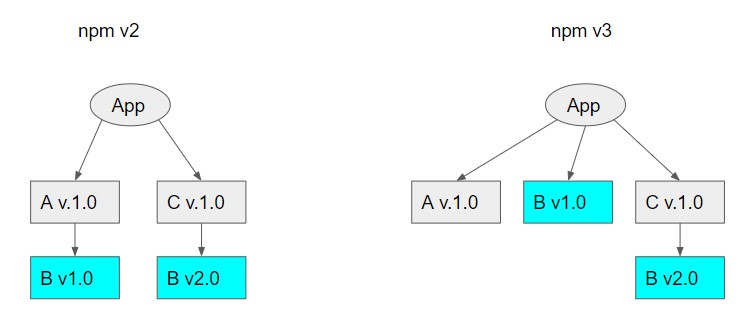
\includegraphics[width=.8\textwidth]{book/chapter-promisesandperils/pics/nestedv2.jpg}
	\caption{Difference between flat and nested dependencies}
	\label{fig:nest}
\end{figure}

\smallskip\noindent\textbf{Peril 5.}\textit{
Developers might declare a dependency to other parts of a software package ecosystem but not use it, e.g., because they failed to update its removal.
}\\

It is common for developers to declare dependencies on other parts of the software package ecosystem but not always use them. This can happen for various reasons, such as forgetting to remove the dependency after it is no longer needed. This can pose a challenge for researchers who are trying to extract dependencies from package managers, like those in configuration files, as there may be inconsistencies between the listed dependencies and what is actually being compiled and used by the code. This can lead to a biased understanding of the software package ecosystem and the relationships between software components.

To address this issue, there have been numerous efforts to track the actual library dependencies compiled and executed in software systems. These efforts aim to provide a more accurate understanding of the dependencies and the relationships between software components. For example, research has been conducted on the use of dynamic analysis to track compiled dependencies in real time and on the development of tools to automatically detect and track executed dependencies \cite{Zapata:ICSME2018, Ponta2018,Chinthanet:ASE2020}.

\subsection{Defining Boundaries and Completeness}

\smallskip\noindent\textbf{Promise 3.}\textit{
Researchers can use the boundaries of software package ecosystems to study communities of developers, e.g., developers contributing to and/or benefiting from the npm ecosystem.
}\\

Following Promise 2, the emergence of package managers has also led to studies that approximate software communities.
Using the libraries.io dataset, researchers were able to study projects that host libraries that use package managers.
Researchers have used this dataset to compare different library ecosystems \cite{kikas.2017,decan:emse:2019,CogoDown2019}.


\smallskip\noindent\textbf{Peril 6.}\textit{
Package managers do not always represent software package ecosystems, their communities, or their sub-communities, e.g., in cases where multiple package managers exist.
}\\

Package managers are a fundamental aspect of software package ecosystems, but do not always fully represent the complex relationships and interactions that occur within a community of developers and users, as shown in Table~\ref{tab:PM_features}. In some cases, multiple package managers exist for the same programming language, creating a complex landscape of software libraries and dependencies that are not always easily understood. For instance, Bower and Meteor manage npm libraries, which can lead to confusion and overlap in the management of dependencies.

Similarly, Java, Scala, Android, and other Java-based open source communities all use the Maven package manager, but each of these communities has its own unique set of libraries, dependencies, and development practises. Researchers should be aware of the limitations of package managers when studying software package ecosystems, and consider the broader context and relationships that exist within these communities. 

\smallskip\noindent\textbf{Peril 7.}\textit{
Lack of activity in parts of a software package ecosystem does not necessarily indicate project failure, e.g., when highly depended-upon libraries are feature-complete.
}\\

It is important to note that lack of activity in a part of a software package ecosystem does not always mean project failure \cite{coelho2017modern}. In some cases, highly relied-upon libraries that have reached feature-completeness may see little activity, but continue to be used by the software community. 

However, it is still important to consider the long-term sustainability of these libraries, especially given the rate at which technology and software development practises change. This has become a topic of interest in recent years, and researchers have explored best practises for sustaining open source projects and ensuring their continued success \cite{Ait2022,valiev2018ecosystem}. Understanding the factors that contribute to project sustainability is important to ensure the longevity and continued growth of software package ecosystems.

\smallskip\noindent\textbf{Peril 8.}\textit{
Sampling from a software package ecosystem is challenging since sub-setting might alter the dependency network, e.g., by breaking dependency chains.
}\\

Sampling from a package ecosystem is not straightforward, as the sample composition can be significantly affected due to missing dependency links between libraries. For instance, a subset of the ecosystem might alter the dependencies between libraries, leading to the breakdown of the dependency chains. This could lead to an incomplete picture of the software package ecosystem, leading to incorrect conclusions from a study. To minimise this risk, researchers should carefully consider the boundaries of their study and choose the appropriate sampling method based on the research questions and goals. For example, researchers could focus on popular, highly dependent, or risk-vulnerable aspects of the ecosystem as a starting point. 
For some ecosystems, the number of downloads, GitHub stars, and watchers are other aspects for the researcher to utilise.


\smallskip\noindent\textbf{Peril 9.}\textit{
Sampling from a software package ecosystem is challenging since the dependency network changes over time, e.g., when dependencies are added, removed, upgraded, or downgraded.
}\\

The dynamic nature of package ecosystems and the constant changes to their dependencies can impact the generalisability of the results. Therefore, it is important to also consider the time granularity of the analysis. For example, if the goal is to understand the evolution of dependencies over time, a finer time granularity may be necessary to capture the smaller changes and trends. However, if the goal is to understand the overall structure and relationships within the ecosystem, a coarser time granularity may be sufficient. Based on recent studies \cite{wattanakriengkrai2022giving,valiev2018ecosystem,Mirsaeedi:icse2020, Brindescu:emse2020, Nassif:icsme2017}, a three-month window seems appropriate for some studies.
Another level of granularity to consider is the size of the component. For instance, there are cases where a single package may contain more than one repository, especially for large library frameworks. 
The granularity also depends on the nature of the ecosystem itself. For instance, researchers should understand whether the ecosystem comprises library packages (e.g., PyPI), plugins (e.g., Eclipse), or is a library distribution (e.g., Android).



\subsection{Analysing and Visualising the Data}

\textbf{Peril 10.}\textit{
Analysing and visualising entire software package ecosystems is challenging due to their size, e.g., in terms of nodes and edges in the network.
}\\

The size of software package ecosystems implies large data sets, which can be overwhelming for tools and algorithms to analyse and display. Therefore, it may be necessary to make choices about the granularity of the data included in the analysis and visualisation. Another alternative is to focus on the most critical parts of the software package ecosystem, such as the high-level structure, highly dependent packages, or parts of the system that pose a risk to security and reliability. 
The key is to strike a balance between detail and simplicity, providing a meaningful representation of the ecosystem while being able to handle the complexity of its size.


\section{Application: When to Apply Which Peril}
\label{PPM:sec:application}

We include a disclaimer stating that not all perils are applicable to every mining situation. To demonstrate the practical application of our perils and their mitigation, we present two case studies that involve mining the software package ecosystem. Each case study has a distinct research objective and focusses on a specific dataset to be mined.

\subsection{Two Case Studies}
Table \ref{tab:cases} presents the two case studies we have selected for this analysis.
The \textit{first case} involves mining for contributions congruent to dependency updates \cite{wattanakriengkrai2022giving}. 
In this work, the authors mine GitHub repositories for Pull Requests and Issues that were submitted and merged congruent to dependency updates within the npm ecosystem. 
The \textit{second case} involves mining communication data for the Eclipse ecosystem \cite{Nugroho2021}. Although the second case does not mine for dependency relations (i.e., use relations),  we show that these perils still apply when mining for other relationships in an ecosystem.
Moreover, the second case studies the Eclipse ecosystem, which is a different dataset compared to the more popular GitHub dataset.

\subsection{Applying Perils and their Mitigation Strategies}
Table \ref{tab:perilsapp} provides a summary of the perils that can be applied to each of the case studies. We will now go into the details of mitigation strategies based on these perils. 
For better organisation and understanding, we have grouped the perils according to the four logical processes for mining.

\smallskip\noindent\textbf{Information to Mine}. 
The first set of mitigation strategies, which addresses perils 1-3, focusses on planning which information to mine. There are two primary strategies that researchers can employ:


\begin{enumerate}
    \item Researchers should use research tools and techniques to remove noise and other biases in the dataset, such as bot detection and the handling of multiple identities. This strategy was implemented in both case studies, as contributions and discussions often have the potential to involve bots or developers with multiple identities.
\item Depending on the research goals, researchers should recognise that not all contributions are equal and filter the dataset accordingly.
\end{enumerate}

We applied these two strategies to both cases. In the first case, the goal was to capture all congruent contributions, so we filtered out contributions made to libraries without dependencies. Since all npm packages are listed in the registry, Peril 3 (private activities) did not apply.
In the second case, we addressed Peril 1 by conducting a qualitative analysis to ensure that the member identities were not duplicated, as Eclipse developers were known to change identities. To mitigate Peril 2, we removed bot responses. For the second case, since all forum data is made public, Peril 3 did not apply.


\begin{table}
\centering
\caption{Description of the research objectives and datasets for the case studies}
 \label{tab:cases}
\begin{tabular}{lp{5cm}r} 
\toprule
\textbf{Case Study} & \textbf{Research Objective}                                                          & \textbf{Datasets}           \\
\midrule
Wattanakriengkrai \etal \cite{wattanakriengkrai2022giving}             & Explore code contributions between library and client (i.e, use-relations)  & libraries.io\\
& &  GitHub API \\
Nugroho \etal \cite{Nugroho2021}                & Explore discussion contributions between contributors (i.e., contributions) & Eclipse API                \\
\bottomrule
\end{tabular}
\end{table}

\begin{table}
\centering
\caption{Application of each peril to the case studies}
 \label{tab:perilsapp}
\begin{tabular}{rp{8cm}ccc} 
\toprule                   
& \textbf{Perils}       & case 1      & case 2                 \\
                                                                               & & npm  & Eclipse   \\
\midrule
\textbf{P1} &Developers might use different identifiers when contributing to different parts of a software package ecosystem, e.g., when contributing to different libraries.                             &    \CheckedBox         &          \CheckedBox           \\ 
%\hline
\textbf{P2} & Developers' contributions to software package ecosystems might be interspersed with bot contributions, e.g., automated dependency updates.                                                      &      \CheckedBox               &      \CheckedBox               \\ 
%\hline
\textbf{P3} & Not all developer activities in software package ecosystems are accessible to the public, e.g., library use in proprietary settings.                                                         &         -           &      \CheckedBox               \\ 
%\hline
\textbf{P4} & Different software package ecosystems define the concept of \`{}\`{}dependency'' differently, e.g., by allowing or not allowing different versions of a library on the same dependency tree. &         \CheckedBox       &     -                            \\ 
%\hline
\textbf{P5} & Developers might declare a dependency to other parts of a software package ecosystem but not use it, e.g., because they failed to update its removal.                                        &     -           &  -    \\
%\hline
\textbf{P6} &Package managers do not always represent software package ecosystems, their communities, or their sub-communities, e.g., in cases where multiple package managers exist.                     &     -                   &  -                  \\
%\hline
\textbf{P7} & Lack of activity in parts of a software package ecosystem does not necessarily indicate project failure, e.g., when highly depended-upon libraries are feature-complete.                     &       \CheckedBox         &  -                           \\
%\hline
\textbf{P8} &Sampling from a software package ecosystem is challenging since sub-setting might alter the dependency network, e.g., by breaking dependency chains.                                         &        \CheckedBox        &     \CheckedBox                                \\
%\hline
\textbf{P9} &Sampling from a software package ecosystem is challenging since the dependency network changes over time, e.g., when dependencies are added, removed, upgraded, or downgraded.               &       \CheckedBox         &     -                          \\
%\hline
\textbf{P10} &Analysing and visualising entire software package ecosystems is challenging due to their size, e.g., in terms of nodes and edges in the network.                                  &        \CheckedBox      &      \CheckedBox               \\
\bottomrule
\end{tabular}
\end{table}

\smallskip\noindent\textbf{Defining Dependencies}. 
The second set of perils (Perils 4-5) is related to dependency relationships between software units, and only the first case study is applicable. To address these perils, researchers should adopt the following strategy:

\begin{enumerate}
    \item Researchers should not rely solely on listed dependencies in configuration files (e.g., pom.xml, package.json, etc.) as a measure of dependency between two components. Instead, code-centric approaches should be used to validate which libraries are actually depended upon.
\end{enumerate}

For example, in the first case, in addition to mining the configuration information, the authors also analysed the similarity of the source code contributions to address Peril 4. Regarding Peril 5, since the study's objective was to investigate changes to the configuration files, the risk of the update not being executed was deemed less important.
It is important to note that the second case study did not include dependency analysis and, therefore, these perils did not apply.

\begin{figure*}[]
    \centering
    \begin{subfigure}{0.9\linewidth}
         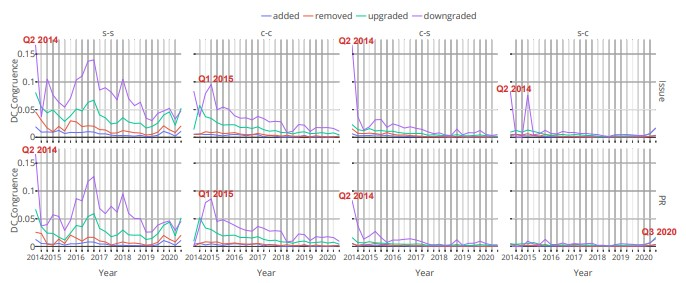
\includegraphics[width=1.1\textwidth]{book/chapter-promisesandperils/pics/congruentViz.jpg}
         \caption{Visualization of a Time analysis for 107,242 libraries.}
     \end{subfigure}
     \begin{subfigure}{0.9\linewidth}
         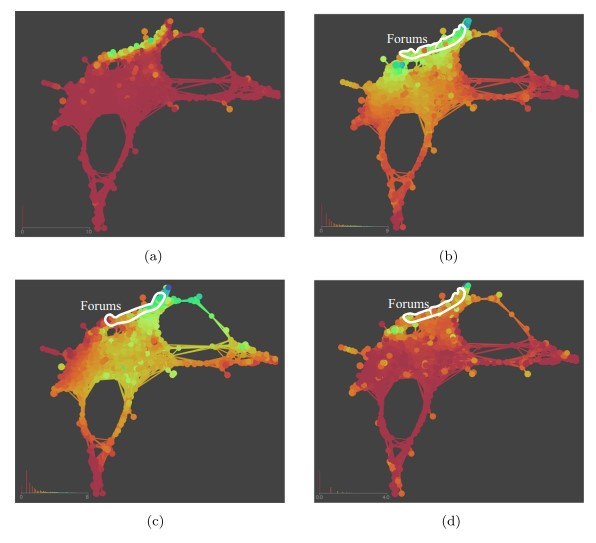
\includegraphics[width=1\textwidth]{book/chapter-promisesandperils/pics/eclipseViz.jpg}
         \caption{A Visual Topology map for 832,058 threads}
     \end{subfigure}
    \caption{Visualisation examples for the two case studies}
    \label{fig:visCase}
\end{figure*}

\smallskip\noindent\textbf{Defining Boundaries}.
The third set of perils (Perils 6-9) is related to the definition of boundaries and completeness and is relevant for both case studies. To mitigate these perils, we recommend the following strategies:

\begin{enumerate}
    \item Researchers should recognise that a dormant project does not necessarily mean that it is inactive. Instead, studies can use alternative heuristics, such as the number of dependents and dependencies, as better indicators of a project's importance in the ecosystem.
    \item Researchers should not rely solely on the programming language to define sub-communities. Using a common package manager for the programming language is a more effective rule of thumb for distinguishing boundaries.
    \item Researchers should avoid random sampling. Instead, sampling should be tailored to the research goals by considering factors such as an appropriate time window or focussing on specific attributes of components (e.g., most dependents, most popular, most contributors).
\end{enumerate}


Peril 6 did not apply to any of the case studies. 
Particularly for the first case, since the goal was to explore the npm package ecosystem, we assumed that the boundaries were clearly defined by the npm registry. 
Similarly, the second case study used the generic Eclipse platform as the boundary. 
Peril 7 was applied to the npm study, while Peril 8 was applied to both case studies. 
As a result, the two cases conducted a qualitative analysis of the dataset to gain deeper insights.
In the first case study, a three-month time window was created to capture dependencies. 
For the second case study, forum contributors were sampled into three groups (i.e., junior, member, or senior) according to the sliding window of their contributions. 

\smallskip\noindent\textbf{Visualisation}.
The final peril (Peril 10) relates to visualisation, which can be challenging due to the vast size and complexity of software ecosystems. As it is not feasible to visualise every aspect of an ecosystem simultaneously, a focused approach is necessary. A mitigation strategy is to select specific attributes of the ecosystem (e.g., the most dependent, most popular, and most contributions) that align with the research needs and objectives. 

Figure \ref{fig:visCase} shows two cases where visualizations are employed to gain insights, especially for large datasets.
In the first figure (a), we visualize the distributions of the data set and applied the appropriate statistical tests, along with the effect size, to test our hypotheses and answer research questions. 
In the second example (b), although not directly related to package ecosystems, the authors utilized a topological visualization \cite{Lum2013ExtractingIF} to gain insights on the over 800,000 forum threads of discussions. 



\section{Chapter Summary}
In this chapter, we explore the various aspects of mining information from the software package ecosystem, presenting three promises and ten perils that researchers should be aware of when undertaking such tasks. The chapter is structured around four key processes for mining: 1) Planning what Information to Mine, 2) Defining Components and their Dependencies, 3) Defining Boundaries and Completeness, and 4) Analysing and Visualising the Data. To help new and experienced researchers navigate these challenges, we introduced the SUG model, which can serve as a valuable tool to minimise threats to validity. Although some perils may be more relevant to specific research objectives, our aim is to equip researchers with the knowledge and resources needed to confidently gather and integrate software package ecosystem data into their work.
%Software library recommendation and usage analysis
% %Semantic labeling three-letter-code: SLU (e.g. \chapter{SLU})

% 
\title{Promises and Perils of Mining \\ Software Package Ecosystem Data}
\author{Raula Gaikovina Kula \and Katsuro Inoue \and Christoph Treude}
\institute{Raula Gaikovina Kula \at Nara Institute of Science and Technology, Japan, \email{raula-k@naist.jp}
\and Katsuro Inoue \at Nanzan University, Japan \email{ inoue599@nanzan-u.ac.jp}
\and  Christoph Treude \at The University of Melbourne, Australia \email{christoph.treude@unimelb.edu.au}}

\maketitle
\label{PPM:ch}
\abstract*{The use of third-party packages is becoming increasingly popular and has led to the emergence of large software package ecosystems with a maze of inter-dependencies. Since the reliance on these ecosystems enables developers to reduce development effort and increase productivity, it has attracted the interest of researchers: understanding the infrastructure and dynamics of package ecosystems has given rise to approaches for better code reuse, automated updates, and the avoidance of vulnerabilities, to name a few examples. But the reality of these ecosystems also poses challenges to software engineering researchers, such as: How do we obtain the complete network of dependencies along with the corresponding versioning information? What are the boundaries of these package ecosystem? How do we consistently detect dependencies that are declared but not used? How do we consistently identify developers within a package ecosystem? How much of the ecosystem do we need to understand to analyse a single component? How well do our approaches generalise across different programming languages and package ecosystems? In this chapter, we review promises and perils of mining the rich data related to software package ecosystems available to software engineering researchers.}

\abstract{The use of third-party packages is becoming increasingly popular and has led to the emergence of large software package ecosystems with a maze of inter-dependencies. Since the reliance on these ecosystems enables developers to reduce development effort and increase productivity, it has attracted the interest of researchers: understanding the infrastructure and dynamics of package ecosystems has given rise to approaches for better code reuse, automated updates, and the avoidance of vulnerabilities, to name a few examples. But the reality of these ecosystems also poses challenges to software engineering researchers, such as: How do we obtain the complete network of dependencies along with the corresponding versioning information? What are the boundaries of these package ecosystems? How do we consistently detect dependencies that are declared but not used? How do we consistently identify developers within a package ecosystem? How much of the ecosystem do we need to understand to analyse a single component? How well do our approaches generalise across different programming languages and package ecosystems? In this chapter, we review promises and perils of mining the rich data related to software package ecosystems available to software engineering researchers.}

%%%%%%%%%%%%%%%%%%%%%%%%%%%%%%%%%%%%%%%%%%%%%%%%%%%%%%%%%%%%%%%%%%

\section{Introduction}
\label{PPM:sec:definition}

Third-party libraries are a great way for developers to incorporate code without having to write their own for every functionality required. By using these libraries, developers can save time and energy while still getting the functions they need.
Using third-party libraries is becoming increasingly popular and has led to the emergence of large software package ecosystems such as npm. While these ecosystems offer many benefits, they also come with risks, such as software vulnerability attacks \cite{Chinthanet:ASE2020}.

Large software package ecosystems are a treasure trove for researchers who can investigate a wide range of questions. For example, by studying activity in large ecosystems, researchers can identify which libraries are the most popular and learn what characteristics make them successful \cite{kikas.2017,decan:emse:2019}.
Additionally, research on large ecosystems can help developers understand how to protect their code from malicious actors who may attempt to exploit vulnerabilities or insert malware into popular libraries.
Studying large software package ecosystems can help us better understand the dynamics of open source development in general. Open source development is a complex process that involves many different stakeholders working together (or sometimes competing) to create valuable code that anyone can use or improve upon. By understanding how these interactions play out in different types of ecosystem structures -- including those with many small projects versus few very large ones -- we can develop insights that might be applicable more broadly across other types of collaborative systems.

In this chapter, we identify and discuss promises and perils during the mining process, ranging from planning what information to mine from the ecosystem to analysing and visualising the mined data. 
Therefore, the chapter is broken down into these logical processes of mining ecosystem data: 1) Planning what Information to Mine, 2) Defining Components and their Dependencies, 3) Defining Boundaries and Completeness, and 4) Analysing and Visualising the Data.

This chapter is intended for researchers and practitioners who are interested in exploring and exploiting software package ecosystem information from a diverse range of sources that are publicly available. 
We also highlight the pitfalls to consider during the mining process, particularly when these pitfalls could lead to a misinterpretation of the analysis and results. 
The chapter is written in a manner that encourages newcomers who have little or no experience or who are interested in utilising ecosystem data across different disciplines outside of software engineering.
Our goal is to get new researchers quickly accustomed to gathering ecosystem information for their research.


\section{A Component-based Software Ecosystem}

Defined as a component-based software ecosystem, we suggest using the term `software package ecosystem' as a suitable term for the symbiotic relationships among third-party library components (as software projects or repositories), as these libraries and their dependent clients coexist on the same technological platform, therefore sharing the same environment and other internal and external factors (e.g., security threats, sharing contributions, etc.).
Please refer to the Introduction chapter for an in-depth definition of the different types of software ecosystems.
We present our interpretation of the software package ecosystem in Kula et al.~\cite{KulaSANER18}, where we formally define a package ecosystem using a Software Universe Graph (SUG).
This is modelled as a structured abstraction of the evolution of software systems and their library dependencies over time.

%%%%%%%%%%%%%%%%%%%%%%%%%%%%%%%%%%%%%%%%%%
\begin{figure*}
	\centering
	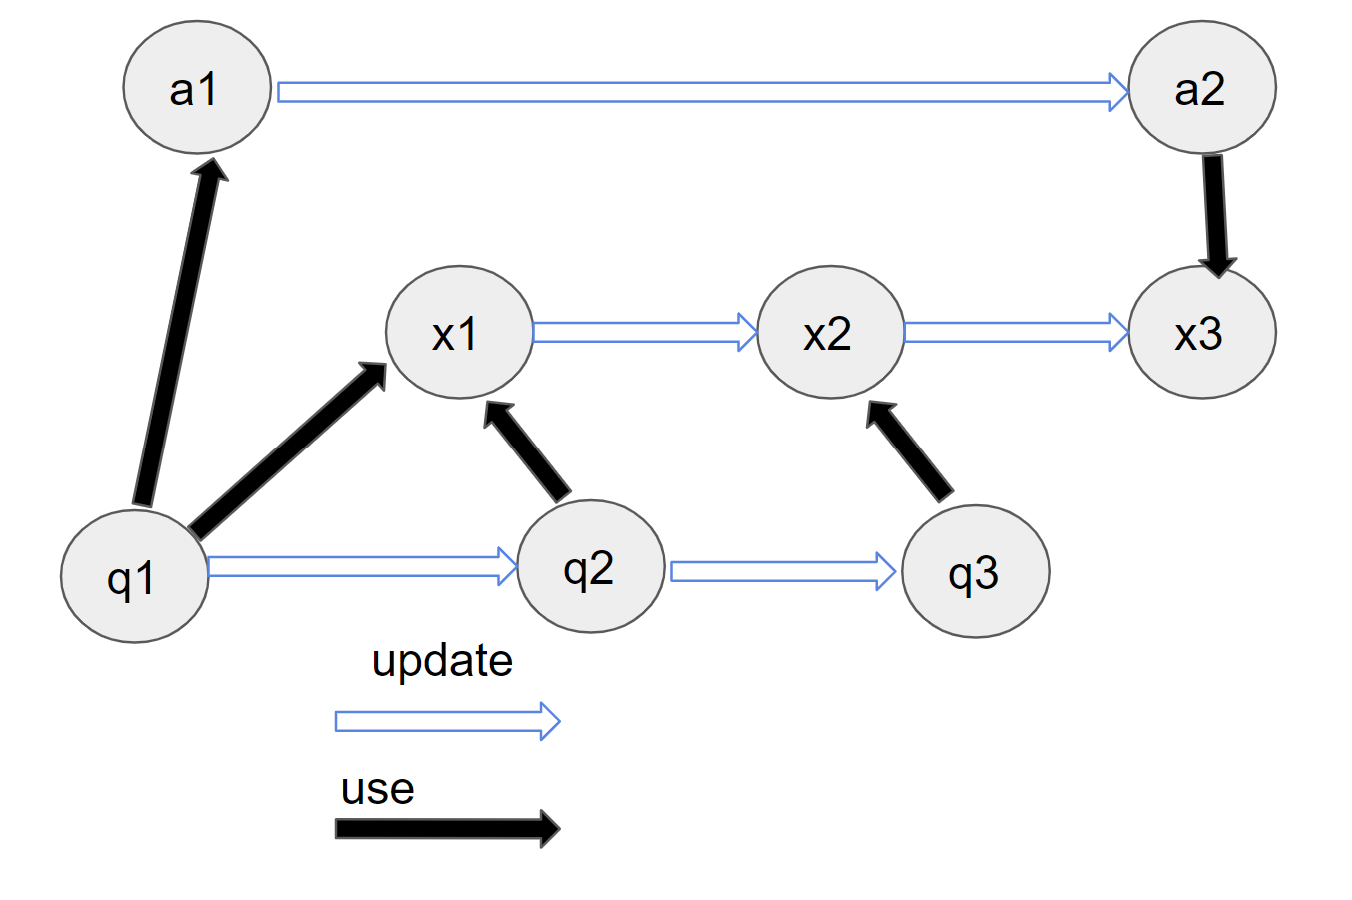
\includegraphics[width=.7\textwidth]{book/chapter-promisesandperils/pics/UniversalExample.jpg}
	\caption{Conceptual example of the Software Universe Graph, depicting the use and update relationships between different software units.}
	\label{fig:SUG}
\end{figure*}
%%%%%%%%%%%%%%%%%%%%%%%%%%%%%%%%%%%%%%%%%%%%%


\paragraph{\textbf{Component-based Representation as a Software Universe Graph}}
\label{PPM:sec:SUG}

First introduced by Kula et al.~\cite{KulaSANER18}, the \textit{Software Universe Graph} (SUG) is a structural abstraction of the software ecosystem of third-party libraries.
Figure \ref{fig:SUG} provides an illustration of the different relationships within the graph.
Let $G= (N,E)$ represent a graph $G$. $N$ is a set of nodes, each node representing a software unit. 
We define a software unit as a version instance of any software program. 

The authors then present the \textit{use} and \textit{update} relationships that exist in the ecosystem.
Hence, the edges $E$ are composed of $E_{use}$ and $E_{update}$. $E_{use}$ is a set of \textit{use-relations} and $E_{update}$ is a set of \textit{update-relations}.

\begin{definition}
An edge $u \rightarrow v \in E_{use}$ means that $u$ uses $v$. The defined functions of $E_{use}$ are:

\begin{equation}
\small
\small \use(u)\equiv \{v|u \rightarrow v\}
\normalsize
\end{equation}
\begin{equation}
\small
\small \useBy(u)\equiv \{v|v \rightarrow u\}
\normalsize
\end{equation}
\end{definition}

Use-relations can be extracted from either the source code or configuration files. 
As shown in Figure \ref{fig:SUG}, node $a1$ uses node $x1$. 
In addition, node $x1$ is used by nodes $a1$, $q1$, and $q2$. Parallel edges for node pairs are not allowed.

\begin{definition}
We represent an update relation from node $a$ to $b$ using $ a \Rightarrow b $, which means that the newer update $b$ was released from node $a$ and is defined as:
\begin{equation}
\small a \Rightarrow b \in E_{update}
\end{equation}
\end{definition}

Update relations refer to when a successive release of a software unit is made available. Figure \ref{fig:SUG} shows that node $q1$ is first updated to node $q2$. Later, node $q2$ is updated to the latest node $q3$. Hence, $q1 \Rightarrow q2 \Rightarrow q3$.
Note that an update should not be confused with forking. 
We distinguish a fork as a separate software unit. 
Each node in the SUG should be denoted by three attributes: \texttt{<name,release,time>}.  
For a node $u$, we define:

\begin{itemize}
	\item \textbf{u.name} Name is the string representation identifier of a software unit.
	We introduce the name axiom: For nodes $u$ and $v$, if $u \Rightarrow v$, then $u.name = v.name$ holds.
	
	\item \textbf{u.release}. Release refers to the specific assigned change reference for a software unit. For nodes $u$ and $v$, if $u \Rightarrow v$
	then $v$ is the immediate successor of $u$. Note that the versioning pattern may vary from project to project. 
	\item \textbf{u.time}. Time refers to the time stamp at which node $u$ was released. For nodes $u$ and $v$ of $u \Rightarrow v$, $u.time < v.time$.
\end{itemize}

\begin{figure}
	\centering
	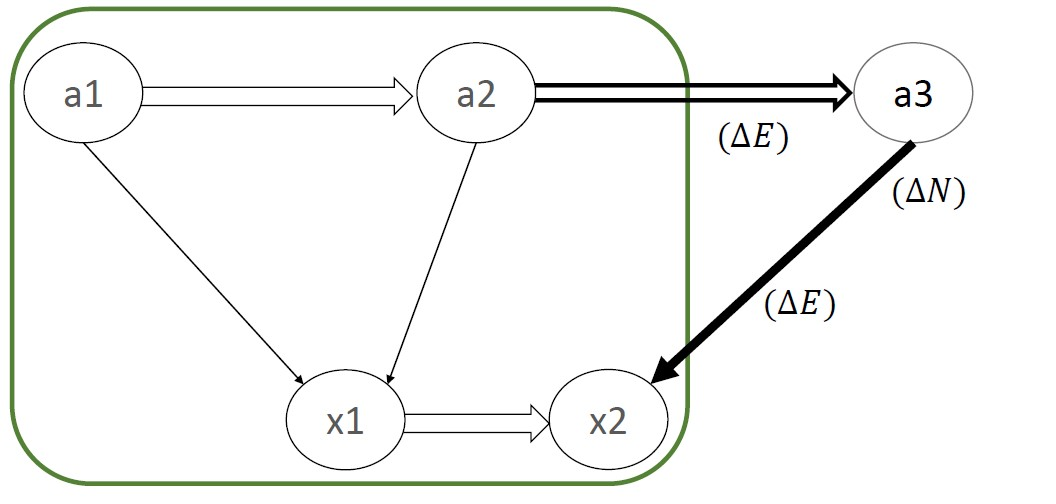
\includegraphics[width=.8\textwidth]{book/chapter-promisesandperils/pics/TemporalSUG.jpg}
	\caption{Temporal property of the SUG}
	\label{fig:SUGTemp}
\end{figure}

\begin{definition}
    
	The SUG has temporal properties.
This describes the simultaneity or ordering in reference to time. Let SUG $G = (N, E) $ be at time $t$. At time $t^{\prime} > t$, we observe an extension of $G$, such that:

\begin{equation}
\small G^{\prime} = (N \cup \Delta N, E \cup \Delta E)
\end{equation}
where $\Delta E \cap (N \times N) = \emptyset$
\end{definition}

Figure \ref{fig:SUGTemp} illustrates the temporal properties of the SUG. 
Here, it is observed that $G'$ is composed of $G$ augmented with newly added node $a3$ and its corresponding $a3 \rightarrow x2$ and $a2 \Rightarrow a3$ relations.
A SUG grows monotonically over time with only additions.
Here, we consider that modification or deletion changes on the SUG do not occur. 

\begin{definition}
    A timed SUG specifies the state of the SUG at any point in time.
So for an SUG $G=(N,E)$, we represent a timed SUG $G_{t}$ at time $t$ as a sub-graph of $G$. Formally,
\begin{equation}
\small G_t\equiv(N_{t}, E_{t})
\end{equation}
where $N_{t} = \{u|u \in N, u.time \leq t \}$ and $E_t = \{ e | e \in E \wedge e \in  N_t \}$
\end{definition}
	


\section{Data Sources}
Researchers can use various datasets to model the ecosystem using the SUG model of usage and update relationships.
The most obvious data source that has revolutionised data mining in the software engineering domain is the GitHub platform. 
Established in 2008, and then purchased by Microsoft in 2020, GitHub is home to various popular Open Source Software. 
GitHub is built on the git version control system and is useful for storing all changes made to a repository. 
In the case of the SUG, a GitHub repository can represent one software unit, whose depend relations can be extracted via a configuration file (such as the package.json file for JavaScript projects).
The repository should also contain the release information that holds the update relations.
Due to its large size, researchers and the GitHub team have made available datasets for researchers to mine, for example through the GitHub API/Graph QL.\footnote{\url{https://docs.github.com/en/graphql}} This is the backend Application Programming Interface (API) that can be used to query large amounts of data on GitHub. Most researchers use the API to download and mine information from the GitHub platform. 
It is important to note that while GitHub introduced a new feature of Dependency Graphs to map the depend relationship,\footnote{\url{https://docs.github.com/en/code-security/supply-chain-security/understanding-your-software-supply-chain/about-the-dependency-graph}} most older projects do not have this feature.
In this case, the researcher would need to manually extract and query the configuration files for dependency information. 

We refer to the first chapter for additional information on data sources for mining software ecosystems. 

\section{Promises and Perils}
\label{PPM:sec:promisesperils}

Using the SUG model of depend and use relations and the available datasets, we can now present our promises and perils of mining ecosystem information.

\subsection{Planning What Information to Mine}

\textbf{Promise 1.}\textit{
Researchers can access and link heterogeneous data related to software package ecosystems, e.g., package registries and bug trackers.}\\

When planning what information to mine from the ecosystem, researchers do not need to limit themselves to the usage and update relationship information.
Platforms that host software repositories include other software management systems such as bug trackers.
For example, GitHub allows researchers to manage GitHub Pull Requests, Issues, and Discussions not only for one project, but for multiple projects.
GitHub provides three management systems that are related to a software repository:

\begin{itemize}
    \item \textit{GitHub Discussions}\footnote{\url{https://docs.github.com/en/discussions}} - The GitHub Discussions forum is a collaborative communication forum for the community around an open source or internal project. Community members can ask and answer questions, share updates, have open-ended conversations, and follow along on decisions affecting the community's way of working.
    \item \textit{GitHub Pull Requests}\footnote{\url{https://docs.github.com/en/pull-requests}} - Pull Requests allow other developers from an ecosystem to make a contribution to a software repository. Pull requests also allow maintainers to discuss and review potential changes with collaborators and add follow-up commits before changes are merged into the software.
    \item \textit{GitHub Issues}\footnote{\url{https://docs.github.com/en/issues}} - Issues are used to track ideas, feedback, tasks, or bugs for work on GitHub.
\end{itemize}

These three systems are examples of how developers contribute to both their own and other projects. 
Hence, to incorporate this information, we can extend the SUG model, creating a model that includes a contribution relationship \cite{wattanakriengkrai2022giving}.

% Note that other platforms may also have management systems, like GitLab, BitBucket and Eclipse.

\begin{definition}
	A Dependency-Contribution graph incorporates contributions by developers whose libraries are involved in dependency relationships. 
\end{definition}

In this work \cite{wattanakriengkrai2022giving}, the authors explore the congruence between dependency updates and developer contributions, based on the original concept of social-technical congruence \cite{stcCataldo2008} where developers contribution patterns are congruent with their coordination needs. Hence, the goal is to identify contributions that are congruent to dependency updates.
As shown in Figure \ref{fig:lib} the authors extend from the typical SUG graph model where $lib_i$ depends (use) on  $lib_k$ and  $lib_j$, while  $lib_j$ also depends on $lib_k$, to the example shown in Figure \ref{fig:dc-graph}.
Different to the SUG, the graph captures developers and their contributions (i.e., the square as $dev_x$ and $dev_y$ represent two different developers making a contribution).
Here contributions are defined as $c$ (Pull Request or Issue) that were submitted to both a library and the client that depends on that library.
Hence, the graph can show contributions that are congruent to dependency changes for a software unit. 

\begin{figure}[t]
     \centering
     \begin{tikzpicture}[
         roundnode/.style={circle, fill=black, minimum size=5mm},
        squarenode/.style={fill=black, text=red, minimum size=5mm},
     ]
    \begin{scope}
         \node[roundnode, label=above:$lib_i$] (s2_proji) at (3, 2.5) {};
        \node[roundnode, label=below:$lib_j$] (s2_projj) at (4,0) {};
         \node[roundnode, label=below:$lib_k$] (s2_projk) at (2,0) {};
     \end{scope}

     \begin{scope} [every edge/.style={draw=gray, very thick}]
         \path [->] (s2_proji) edge (s2_projj);
         \path [->] (s2_proji) edge (s2_projk);
         \path [->] (s2_projj) edge (s2_projk);
     \end{scope}
     \end{tikzpicture}
    
     \caption{Example dependency graph for a given time period}
     \label{fig:lib}
     \vspace{2ex}
 \end{figure}
\begin{figure}[t]
    \centering

    \begin{tikzpicture}[
        roundnode/.style={circle, fill=black, minimum size=5mm},
        squarenode/.style={fill=black, text=red, minimum size=5mm},
    ]
    \begin{scope}
        
        \node[roundnode, label=right:$lib_i$] (s2_proji) at (4, 1.5) {};
        \node[roundnode, label=below:$lib_j$] (s2_projj) at (5,0) {};
        \node[roundnode, label=below:$lib_k$] (s2_projk) at (3,0) {};
        
        \node[squarenode, label=below:$dev_x$] (s3_devx) at (2, 3.5) {};
        
        \node[squarenode, label=below:$dev_y$] (s3_devy) at (6, 3.5) {};
        
    \end{scope}

    \begin{scope} [every edge/.style={draw=gray, very thick}]
        \path [->] (s2_proji)  edge  (s2_projj);
        \path [->] (s2_proji) edge (s2_projk);
        \path [->] (s2_projj) edge (s2_projk);
        
    \end{scope}
    \begin{scope} [every edge/.style={draw=gray, thick, double distance=2pt}]
        \path [->] (6, 2.8) edge node[left = 2mm] {$contribute$} (s2_proji);
        \path [->] (6, 2.8) edge[bend left=15] node[right = 1mm] {$contribute$} (s2_projj);
        \path [->] (2, 2.8) edge node[right = 2mm] {$$} (s2_proji);
        \path [->] (2, 2.8) edge[bend right=15] node[left = 1mm] {$contribute$} (s2_projk);
    \end{scope}
    \end{tikzpicture}
\end{figure}
\begin{figure}[t]
    \centering
    \begin{tikzpicture}[
        roundnode/.style={circle, fill=black, minimum size=5mm},
        squarenode/.style={fill=black, text=red, minimum size=5mm},
    ]
    \end{tikzpicture}
\caption{Example Dependency-Contribution graph showing relationships between contributions and dependencies}
 \label{fig:dc-graph}
\end{figure}

This is just one example of the type of research that is enabled by access to heterogeneous data related to software package ecosystems.

\smallskip\noindent\textbf{Peril 1.}\textit{
 Developers might use different identifiers when contributing to different parts of a software package ecosystem, e.g., when contributing to different libraries.}\\
 
When modelling using such graphs, there is a threat that contributors may use multiple identifiers (i.e., $c_x$ and $c_y$ are the same contributor).
This is a well-known research problem, and there has been work to merge these accounts, such as \cite{wiese2016mailing}.
GitHub has introduced mechanisms such as two-factor authentication\footnote{\url{https://docs.github.com/en/authentication/securing-your-account-with-two-factor-authentication-2fa/configuring-two-factor-authentication}} to counteract the issue of multiple identifiers.
This is since developers might be less likely to switch accounts if it requires cumbersome authentication.


\smallskip\noindent\textbf{Peril 2.}\textit{
Developers' contributions to software package ecosystems might be interspersed with bot contributions, e.g., automated dependency updates.}\\

The rise of automation and artificial intelligence has led to much work on the integration of automated scheduling (i.e., bots) into software development workflows \cite{Storey2016, Farooq2016, Wessel2018, Erlenhov2019, bot_modify_wf} to name a few. These bots are designed to perform specific tasks within a software package ecosystem. For example, a bot may be programmed to automatically update dependencies, test code changes, or deploy software to production. As an example, the Google APIs repo-automation-bots project lists bots for automated labelling of issues and pull requests, automated approval of pull requests, and triggering releases.\footnote{\url{https://github.com/googleapis/repo-automation-bots}}
Bots perform common maintenance tasks in many software projects and are now commonplace \cite{Beschastnikh2017, Urli2018,BIMAN,bot_or_not}.
Especially with bots such as dependabot (automated pull requests to update configurations to reduce the risk of vulnerability threats),\footnote{\url{https://github.com/dependabot}} more and more automation has caused a lot of noise in the contributions between projects.
There are also bots for communication and documentation \cite{Urli2018, Lin2016, Lebeuf2017a}.

To be able to draw accurate conclusions about what humans are doing in software package ecosystems, researchers should consider distinguishing between bot and human contributions.
It is also important to differentiate this from other contributions \cite{maeprasart2022understanding}.
The research community has responded well, with a wide range of techniques and tools to mitigate this peril \cite{Bodegha2021, golzadeh2022accuracy}.

\smallskip\noindent\textbf{Peril 3.}\textit{
Not all developer activities in software package ecosystems are accessible to the public, e.g., library use in proprietary settings.
}\\

Not all developer activities in software package ecosystems are accessible to the public, e.g., when the boundary between open source and industry is blurred \cite{stol2014inner}, which presents a challenge for researchers who aim to study the development process. This is particularly true in proprietary settings where software development is performed behind closed doors or is open source for a limited time period, thus resulting in the artefacts not permanently being publicly available.
This can make it difficult to understand the broader ecosystem in which a software project is developed.
Proprietary settings may lead to non-standardisation in software development practises. Different software projects may use different management systems and tools, making it difficult to accurately compare and analyse software development activities across various projects. For example, some projects may use communication, documentation, and other management tools not captured on the same platform \cite{montgomery2022alternative}. For example, some projects might use Bugzilla instead of issues and pull requests for their bug and code review systems, while others may use Discord, Slack channels, or email threads for their communication needs.

This lack of standardisation in software development practises presents a challenge for researchers who study the software package ecosystem and understand the development process. To address this issue, researchers should strive to collect data from a diverse set of projects to gain a comprehensive understanding of the software package ecosystem. In addition, researchers may need to adjust their methodologies or data collection techniques to accommodate the different tools and practises used by different software projects.

\subsection{Defining Components and their Dependencies}

\smallskip\noindent\textbf{Promise 2.}\textit{
Researchers can access a software package ecosystem's dependency network through package managers and registries, e.g., npm lists the dependencies and dependents for over a million libraries.}\\


With the rise of curated datasets like libraries.io, researchers can now recover and model dependency relations between software units using pre-extracted datasets.
Table \ref{tab:PM_features} shows examples of popular package managers mined from the libraries.io dataset in 2020. 

\begin{table*}[]
\caption{Summary of 13 package managers from libraries.io as ranked by TIOBE in 2020}
 \label{tab:PM_features}
 \centering
\begin{tabular}{@{}llrlll@{}}
\toprule
\begin{tabular}[c]{@{}l@{}}Package \\ Ecosystem\end{tabular} & \begin{tabular}[c]{@{}l@{}}Programming \\ Language\end{tabular} &  \begin{tabular}[c]{@{}l@{}}Tiobe \\ Rank\end{tabular} & Environment & \begin{tabular}[c]{@{}l@{}}Dependency \\ Tree\end{tabular} & \begin{tabular}[c]{@{}l@{}}Package   \\Archive link\end{tabular}\\ \midrule
PyPI & Python & 2 & Python & Flat & pypi.org  \\
Maven & Java & 3 & JVM & Flat & Maven.org  \\
Bower & JavaScript & 7 & Node.js & Flat & bower.io  \\
Meteor & JavaScript & 7 & Node.js & Nested & atmospherejs.com \\
npm & JavaScript & 7 & Node.js & Nested (v2) & npmjs.com  \\
Packagist & PHP & 8 & PHP & Flat & packagist.org \\
Puppet & Ruby & 13 & Ruby MRI & Flat & forge.puppet.com  \\
RubyGems & Ruby & 13 & Ruby MRI & Flat & rubygems.org  \\
CRAN & R & 14 & RStudio & Flat & cran.r-project.org  \\
CPAN & Perl & 15 & Perl & Flat & metacpan.org  \\
GO & Golang & 20 & Go & Flat & pkg.go.dev  \\
NuGet & C\#, VB & 5, 6 & .NET & Flat & nuget.org \\
Anaconda & Python, R, C\# & 2, 14, 5 & Anaconda & Flat & anaconda.org  \\ \bottomrule
\end{tabular}
\end{table*}

\smallskip\noindent\textbf{Peril 4.}\textit{
Different software package ecosystems define the concept of ``dependency'' differently, e.g., by allowing or not allowing different versions of a library on the same dependency tree.
}\\

Different software package ecosystems have varying definitions of what constitutes a dependency. For example, some ecosystems may allow multiple versions of a library to exist on the same dependency tree, while others may restrict developers to a single version of a library \cite{Islam}. These restrictions are often based on the programming language being used, as different languages have different approaches to managing dependencies. It is important to consider the restrictions on dependency relationships when studying software package ecosystems, as they can have a major impact on the development process. For example, the ability to use multiple versions of a library on the same dependency tree can greatly simplify the process of updating dependencies and can make it easier to resolve conflicts between libraries.

One way to visualise the impact of these restrictions is to compare the difference between a nested dependency tree and a directed dependency tree, as shown in Figure \ref{fig:nest}.\footnote{Taken from \url{https://npm.github.io/how-npm-works-docs/npm3/how-npm3-works.html}} This distinction is important because it highlights the different ways that a software unit can depend on different versions of the same library.
In this example, npm v3 creates the dependency tree based on the installation order, therefore flattening unnecessary nested dependencies (i.e., B v1.0 in cyan). This reduces the complexity of a nested tree by resolving some of the transitive dependencies (nested dependencies).

\begin{figure}
	\centering
	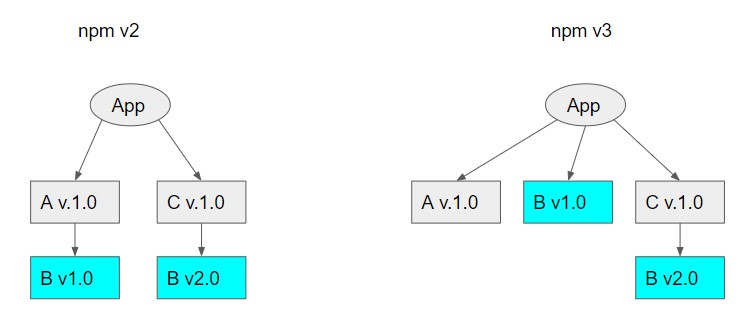
\includegraphics[width=.8\textwidth]{book/chapter-promisesandperils/pics/nestedv2.jpg}
	\caption{Difference between flat and nested dependencies}
	\label{fig:nest}
\end{figure}

\smallskip\noindent\textbf{Peril 5.}\textit{
Developers might declare a dependency to other parts of a software package ecosystem but not use it, e.g., because they failed to update its removal.
}\\

It is common for developers to declare dependencies on other parts of the software package ecosystem but not always use them. This can happen for various reasons, such as forgetting to remove the dependency after it is no longer needed. This can pose a challenge for researchers who are trying to extract dependencies from package managers, like those in configuration files, as there may be inconsistencies between the listed dependencies and what is actually being compiled and used by the code. This can lead to a biased understanding of the software package ecosystem and the relationships between software components.

To address this issue, there have been numerous efforts to track the actual library dependencies compiled and executed in software systems. These efforts aim to provide a more accurate understanding of the dependencies and the relationships between software components. For example, research has been conducted on the use of dynamic analysis to track compiled dependencies in real time and on the development of tools to automatically detect and track executed dependencies \cite{Zapata:ICSME2018, Ponta2018,Chinthanet:ASE2020}.

\subsection{Defining Boundaries and Completeness}

\smallskip\noindent\textbf{Promise 3.}\textit{
Researchers can use the boundaries of software package ecosystems to study communities of developers, e.g., developers contributing to and/or benefiting from the npm ecosystem.
}\\

Following Promise 2, the emergence of package managers has also led to studies that approximate software communities.
Using the libraries.io dataset, researchers were able to study projects that host libraries that use package managers.
Researchers have used this dataset to compare different library ecosystems \cite{kikas.2017,decan:emse:2019,CogoDown2019}.


\smallskip\noindent\textbf{Peril 6.}\textit{
Package managers do not always represent software package ecosystems, their communities, or their sub-communities, e.g., in cases where multiple package managers exist.
}\\

Package managers are a fundamental aspect of software package ecosystems, but do not always fully represent the complex relationships and interactions that occur within a community of developers and users, as shown in Table~\ref{tab:PM_features}. In some cases, multiple package managers exist for the same programming language, creating a complex landscape of software libraries and dependencies that are not always easily understood. For instance, Bower and Meteor manage npm libraries, which can lead to confusion and overlap in the management of dependencies.

Similarly, Java, Scala, Android, and other Java-based open source communities all use the Maven package manager, but each of these communities has its own unique set of libraries, dependencies, and development practises. Researchers should be aware of the limitations of package managers when studying software package ecosystems, and consider the broader context and relationships that exist within these communities. 

\smallskip\noindent\textbf{Peril 7.}\textit{
Lack of activity in parts of a software package ecosystem does not necessarily indicate project failure, e.g., when highly depended-upon libraries are feature-complete.
}\\

It is important to note that lack of activity in a part of a software package ecosystem does not always mean project failure \cite{coelho2017modern}. In some cases, highly relied-upon libraries that have reached feature-completeness may see little activity, but continue to be used by the software community. 

However, it is still important to consider the long-term sustainability of these libraries, especially given the rate at which technology and software development practises change. This has become a topic of interest in recent years, and researchers have explored best practises for sustaining open source projects and ensuring their continued success \cite{Ait2022,valiev2018ecosystem}. Understanding the factors that contribute to project sustainability is important to ensure the longevity and continued growth of software package ecosystems.

\smallskip\noindent\textbf{Peril 8.}\textit{
Sampling from a software package ecosystem is challenging since sub-setting might alter the dependency network, e.g., by breaking dependency chains.
}\\

Sampling from a package ecosystem is not straightforward, as the sample composition can be significantly affected due to missing dependency links between libraries. For instance, a subset of the ecosystem might alter the dependencies between libraries, leading to the breakdown of the dependency chains. This could lead to an incomplete picture of the software package ecosystem, leading to incorrect conclusions from a study. To minimise this risk, researchers should carefully consider the boundaries of their study and choose the appropriate sampling method based on the research questions and goals. For example, researchers could focus on popular, highly dependent, or risk-vulnerable aspects of the ecosystem as a starting point. 
For some ecosystems, the number of downloads, GitHub stars, and watchers are other aspects for the researcher to utilise.


\smallskip\noindent\textbf{Peril 9.}\textit{
Sampling from a software package ecosystem is challenging since the dependency network changes over time, e.g., when dependencies are added, removed, upgraded, or downgraded.
}\\

The dynamic nature of package ecosystems and the constant changes to their dependencies can impact the generalisability of the results. Therefore, it is important to also consider the time granularity of the analysis. For example, if the goal is to understand the evolution of dependencies over time, a finer time granularity may be necessary to capture the smaller changes and trends. However, if the goal is to understand the overall structure and relationships within the ecosystem, a coarser time granularity may be sufficient. Based on recent studies \cite{wattanakriengkrai2022giving,valiev2018ecosystem,Mirsaeedi:icse2020, Brindescu:emse2020, Nassif:icsme2017}, a three-month window seems appropriate for some studies.
Another level of granularity to consider is the size of the component. For instance, there are cases where a single package may contain more than one repository, especially for large library frameworks. 
The granularity also depends on the nature of the ecosystem itself. For instance, researchers should understand whether the ecosystem comprises library packages (e.g., PyPI), plugins (e.g., Eclipse), or is a library distribution (e.g., Android).



\subsection{Analysing and Visualising the Data}

\textbf{Peril 10.}\textit{
Analysing and visualising entire software package ecosystems is challenging due to their size, e.g., in terms of nodes and edges in the network.
}\\

The size of software package ecosystems implies large data sets, which can be overwhelming for tools and algorithms to analyse and display. Therefore, it may be necessary to make choices about the granularity of the data included in the analysis and visualisation. Another alternative is to focus on the most critical parts of the software package ecosystem, such as the high-level structure, highly dependent packages, or parts of the system that pose a risk to security and reliability. 
The key is to strike a balance between detail and simplicity, providing a meaningful representation of the ecosystem while being able to handle the complexity of its size.


\section{Application: When to Apply Which Peril}
\label{PPM:sec:application}

We include a disclaimer stating that not all perils are applicable to every mining situation. To demonstrate the practical application of our perils and their mitigation, we present two case studies that involve mining the software package ecosystem. Each case study has a distinct research objective and focusses on a specific dataset to be mined.

\subsection{Two Case Studies}
Table \ref{tab:cases} presents the two case studies we have selected for this analysis.
The \textit{first case} involves mining for contributions congruent to dependency updates \cite{wattanakriengkrai2022giving}. 
In this work, the authors mine GitHub repositories for Pull Requests and Issues that were submitted and merged congruent to dependency updates within the npm ecosystem. 
The \textit{second case} involves mining communication data for the Eclipse ecosystem \cite{Nugroho2021}. Although the second case does not mine for dependency relations (i.e., use relations),  we show that these perils still apply when mining for other relationships in an ecosystem.
Moreover, the second case studies the Eclipse ecosystem, which is a different dataset compared to the more popular GitHub dataset.

\subsection{Applying Perils and their Mitigation Strategies}
Table \ref{tab:perilsapp} provides a summary of the perils that can be applied to each of the case studies. We will now go into the details of mitigation strategies based on these perils. 
For better organisation and understanding, we have grouped the perils according to the four logical processes for mining.

\smallskip\noindent\textbf{Information to Mine}. 
The first set of mitigation strategies, which addresses perils 1-3, focusses on planning which information to mine. There are two primary strategies that researchers can employ:


\begin{enumerate}
    \item Researchers should use research tools and techniques to remove noise and other biases in the dataset, such as bot detection and the handling of multiple identities. This strategy was implemented in both case studies, as contributions and discussions often have the potential to involve bots or developers with multiple identities.
\item Depending on the research goals, researchers should recognise that not all contributions are equal and filter the dataset accordingly.
\end{enumerate}

We applied these two strategies to both cases. In the first case, the goal was to capture all congruent contributions, so we filtered out contributions made to libraries without dependencies. Since all npm packages are listed in the registry, Peril 3 (private activities) did not apply.
In the second case, we addressed Peril 1 by conducting a qualitative analysis to ensure that the member identities were not duplicated, as Eclipse developers were known to change identities. To mitigate Peril 2, we removed bot responses. For the second case, since all forum data is made public, Peril 3 did not apply.


\begin{table}
\centering
\caption{Description of the research objectives and datasets for the case studies}
 \label{tab:cases}
\begin{tabular}{lp{5cm}r} 
\toprule
\textbf{Case Study} & \textbf{Research Objective}                                                          & \textbf{Datasets}           \\
\midrule
Wattanakriengkrai \etal \cite{wattanakriengkrai2022giving}             & Explore code contributions between library and client (i.e, use-relations)  & libraries.io\\
& &  GitHub API \\
Nugroho \etal \cite{Nugroho2021}                & Explore discussion contributions between contributors (i.e., contributions) & Eclipse API                \\
\bottomrule
\end{tabular}
\end{table}

\begin{table}
\centering
\caption{Application of each peril to the case studies}
 \label{tab:perilsapp}
\begin{tabular}{rp{8cm}ccc} 
\toprule                   
& \textbf{Perils}       & case 1      & case 2                 \\
                                                                               & & npm  & Eclipse   \\
\midrule
\textbf{P1} &Developers might use different identifiers when contributing to different parts of a software package ecosystem, e.g., when contributing to different libraries.                             &    \CheckedBox         &          \CheckedBox           \\ 
%\hline
\textbf{P2} & Developers' contributions to software package ecosystems might be interspersed with bot contributions, e.g., automated dependency updates.                                                      &      \CheckedBox               &      \CheckedBox               \\ 
%\hline
\textbf{P3} & Not all developer activities in software package ecosystems are accessible to the public, e.g., library use in proprietary settings.                                                         &         -           &      \CheckedBox               \\ 
%\hline
\textbf{P4} & Different software package ecosystems define the concept of \`{}\`{}dependency'' differently, e.g., by allowing or not allowing different versions of a library on the same dependency tree. &         \CheckedBox       &     -                            \\ 
%\hline
\textbf{P5} & Developers might declare a dependency to other parts of a software package ecosystem but not use it, e.g., because they failed to update its removal.                                        &     -           &  -    \\
%\hline
\textbf{P6} &Package managers do not always represent software package ecosystems, their communities, or their sub-communities, e.g., in cases where multiple package managers exist.                     &     -                   &  -                  \\
%\hline
\textbf{P7} & Lack of activity in parts of a software package ecosystem does not necessarily indicate project failure, e.g., when highly depended-upon libraries are feature-complete.                     &       \CheckedBox         &  -                           \\
%\hline
\textbf{P8} &Sampling from a software package ecosystem is challenging since sub-setting might alter the dependency network, e.g., by breaking dependency chains.                                         &        \CheckedBox        &     \CheckedBox                                \\
%\hline
\textbf{P9} &Sampling from a software package ecosystem is challenging since the dependency network changes over time, e.g., when dependencies are added, removed, upgraded, or downgraded.               &       \CheckedBox         &     -                          \\
%\hline
\textbf{P10} &Analysing and visualising entire software package ecosystems is challenging due to their size, e.g., in terms of nodes and edges in the network.                                  &        \CheckedBox      &      \CheckedBox               \\
\bottomrule
\end{tabular}
\end{table}

\smallskip\noindent\textbf{Defining Dependencies}. 
The second set of perils (Perils 4-5) is related to dependency relationships between software units, and only the first case study is applicable. To address these perils, researchers should adopt the following strategy:

\begin{enumerate}
    \item Researchers should not rely solely on listed dependencies in configuration files (e.g., pom.xml, package.json, etc.) as a measure of dependency between two components. Instead, code-centric approaches should be used to validate which libraries are actually depended upon.
\end{enumerate}

For example, in the first case, in addition to mining the configuration information, the authors also analysed the similarity of the source code contributions to address Peril 4. Regarding Peril 5, since the study's objective was to investigate changes to the configuration files, the risk of the update not being executed was deemed less important.
It is important to note that the second case study did not include dependency analysis and, therefore, these perils did not apply.

\begin{figure*}[]
    \centering
    \begin{subfigure}{0.9\linewidth}
         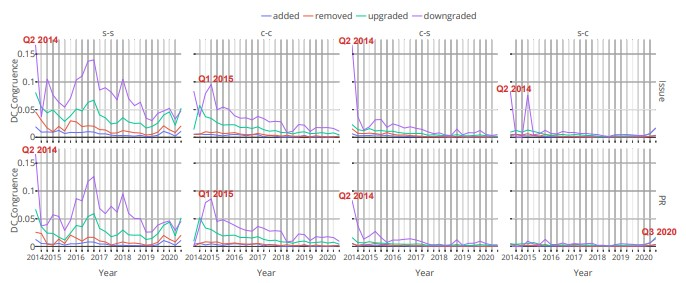
\includegraphics[width=1.1\textwidth]{book/chapter-promisesandperils/pics/congruentViz.jpg}
         \caption{Visualization of a Time analysis for 107,242 libraries.}
     \end{subfigure}
     \begin{subfigure}{0.9\linewidth}
         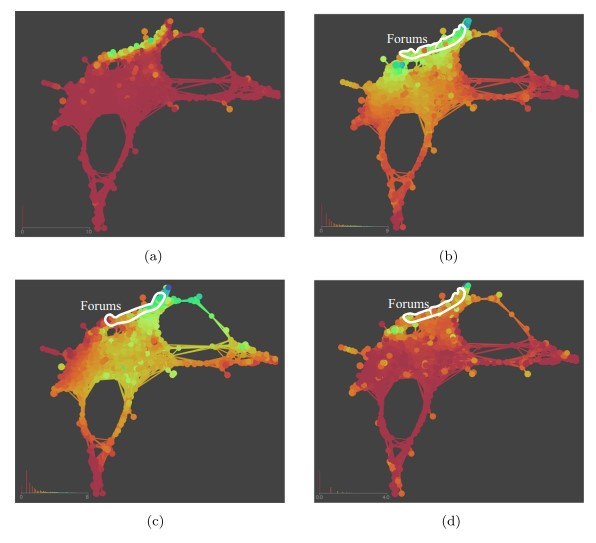
\includegraphics[width=1\textwidth]{book/chapter-promisesandperils/pics/eclipseViz.jpg}
         \caption{A Visual Topology map for 832,058 threads}
     \end{subfigure}
    \caption{Visualisation examples for the two case studies}
    \label{fig:visCase}
\end{figure*}

\smallskip\noindent\textbf{Defining Boundaries}.
The third set of perils (Perils 6-9) is related to the definition of boundaries and completeness and is relevant for both case studies. To mitigate these perils, we recommend the following strategies:

\begin{enumerate}
    \item Researchers should recognise that a dormant project does not necessarily mean that it is inactive. Instead, studies can use alternative heuristics, such as the number of dependents and dependencies, as better indicators of a project's importance in the ecosystem.
    \item Researchers should not rely solely on the programming language to define sub-communities. Using a common package manager for the programming language is a more effective rule of thumb for distinguishing boundaries.
    \item Researchers should avoid random sampling. Instead, sampling should be tailored to the research goals by considering factors such as an appropriate time window or focussing on specific attributes of components (e.g., most dependents, most popular, most contributors).
\end{enumerate}


Peril 6 did not apply to any of the case studies. 
Particularly for the first case, since the goal was to explore the npm package ecosystem, we assumed that the boundaries were clearly defined by the npm registry. 
Similarly, the second case study used the generic Eclipse platform as the boundary. 
Peril 7 was applied to the npm study, while Peril 8 was applied to both case studies. 
As a result, the two cases conducted a qualitative analysis of the dataset to gain deeper insights.
In the first case study, a three-month time window was created to capture dependencies. 
For the second case study, forum contributors were sampled into three groups (i.e., junior, member, or senior) according to the sliding window of their contributions. 

\smallskip\noindent\textbf{Visualisation}.
The final peril (Peril 10) relates to visualisation, which can be challenging due to the vast size and complexity of software ecosystems. As it is not feasible to visualise every aspect of an ecosystem simultaneously, a focused approach is necessary. A mitigation strategy is to select specific attributes of the ecosystem (e.g., the most dependent, most popular, and most contributions) that align with the research needs and objectives. 

Figure \ref{fig:visCase} shows two cases where visualizations are employed to gain insights, especially for large datasets.
In the first figure (a), we visualize the distributions of the data set and applied the appropriate statistical tests, along with the effect size, to test our hypotheses and answer research questions. 
In the second example (b), although not directly related to package ecosystems, the authors utilized a topological visualization \cite{Lum2013ExtractingIF} to gain insights on the over 800,000 forum threads of discussions. 



\section{Chapter Summary}
In this chapter, we explore the various aspects of mining information from the software package ecosystem, presenting three promises and ten perils that researchers should be aware of when undertaking such tasks. The chapter is structured around four key processes for mining: 1) Planning what Information to Mine, 2) Defining Components and their Dependencies, 3) Defining Boundaries and Completeness, and 4) Analysing and Visualising the Data. To help new and experienced researchers navigate these challenges, we introduced the SUG model, which can serve as a valuable tool to minimise threats to validity. Although some perils may be more relevant to specific research objectives, our aim is to equip researchers with the knowledge and resources needed to confidently gather and integrate software package ecosystem data into their work.
%Emotion Analysis in Software Development Ecosystems
% %Semantic labeling three-letter-code: EMO (e.g. \chapter{EMO})


% %%%%%%%%%%%%%%%%%%%%%part.tex%%%%%%%%%%%%%%%%%%%%%%%%%%%%%%%%%%
% 
% sample part title
%
% Use this file as a template for your own input.
%
%%%%%%%%%%%%%%%%%%%%%%%% Springer %%%%%%%%%%%%%%%%%%%%%%%%%%

\begin{partbacktext}
\part{EVOLUTION WITHIN SOFTWARE ECOSYSTEMS}
\label{part:evolution}

\end{partbacktext} %EVOLUTION WITHIN SOFTWARE  ECOSYSTEMS

% 
\title{Promises and Perils of Mining \\ Software Package Ecosystem Data}
\author{Raula Gaikovina Kula \and Katsuro Inoue \and Christoph Treude}
\institute{Raula Gaikovina Kula \at Nara Institute of Science and Technology, Japan, \email{raula-k@naist.jp}
\and Katsuro Inoue \at Nanzan University, Japan \email{ inoue599@nanzan-u.ac.jp}
\and  Christoph Treude \at The University of Melbourne, Australia \email{christoph.treude@unimelb.edu.au}}

\maketitle
\label{PPM:ch}
\abstract*{The use of third-party packages is becoming increasingly popular and has led to the emergence of large software package ecosystems with a maze of inter-dependencies. Since the reliance on these ecosystems enables developers to reduce development effort and increase productivity, it has attracted the interest of researchers: understanding the infrastructure and dynamics of package ecosystems has given rise to approaches for better code reuse, automated updates, and the avoidance of vulnerabilities, to name a few examples. But the reality of these ecosystems also poses challenges to software engineering researchers, such as: How do we obtain the complete network of dependencies along with the corresponding versioning information? What are the boundaries of these package ecosystem? How do we consistently detect dependencies that are declared but not used? How do we consistently identify developers within a package ecosystem? How much of the ecosystem do we need to understand to analyse a single component? How well do our approaches generalise across different programming languages and package ecosystems? In this chapter, we review promises and perils of mining the rich data related to software package ecosystems available to software engineering researchers.}

\abstract{The use of third-party packages is becoming increasingly popular and has led to the emergence of large software package ecosystems with a maze of inter-dependencies. Since the reliance on these ecosystems enables developers to reduce development effort and increase productivity, it has attracted the interest of researchers: understanding the infrastructure and dynamics of package ecosystems has given rise to approaches for better code reuse, automated updates, and the avoidance of vulnerabilities, to name a few examples. But the reality of these ecosystems also poses challenges to software engineering researchers, such as: How do we obtain the complete network of dependencies along with the corresponding versioning information? What are the boundaries of these package ecosystems? How do we consistently detect dependencies that are declared but not used? How do we consistently identify developers within a package ecosystem? How much of the ecosystem do we need to understand to analyse a single component? How well do our approaches generalise across different programming languages and package ecosystems? In this chapter, we review promises and perils of mining the rich data related to software package ecosystems available to software engineering researchers.}

%%%%%%%%%%%%%%%%%%%%%%%%%%%%%%%%%%%%%%%%%%%%%%%%%%%%%%%%%%%%%%%%%%

\section{Introduction}
\label{PPM:sec:definition}

Third-party libraries are a great way for developers to incorporate code without having to write their own for every functionality required. By using these libraries, developers can save time and energy while still getting the functions they need.
Using third-party libraries is becoming increasingly popular and has led to the emergence of large software package ecosystems such as npm. While these ecosystems offer many benefits, they also come with risks, such as software vulnerability attacks \cite{Chinthanet:ASE2020}.

Large software package ecosystems are a treasure trove for researchers who can investigate a wide range of questions. For example, by studying activity in large ecosystems, researchers can identify which libraries are the most popular and learn what characteristics make them successful \cite{kikas.2017,decan:emse:2019}.
Additionally, research on large ecosystems can help developers understand how to protect their code from malicious actors who may attempt to exploit vulnerabilities or insert malware into popular libraries.
Studying large software package ecosystems can help us better understand the dynamics of open source development in general. Open source development is a complex process that involves many different stakeholders working together (or sometimes competing) to create valuable code that anyone can use or improve upon. By understanding how these interactions play out in different types of ecosystem structures -- including those with many small projects versus few very large ones -- we can develop insights that might be applicable more broadly across other types of collaborative systems.

In this chapter, we identify and discuss promises and perils during the mining process, ranging from planning what information to mine from the ecosystem to analysing and visualising the mined data. 
Therefore, the chapter is broken down into these logical processes of mining ecosystem data: 1) Planning what Information to Mine, 2) Defining Components and their Dependencies, 3) Defining Boundaries and Completeness, and 4) Analysing and Visualising the Data.

This chapter is intended for researchers and practitioners who are interested in exploring and exploiting software package ecosystem information from a diverse range of sources that are publicly available. 
We also highlight the pitfalls to consider during the mining process, particularly when these pitfalls could lead to a misinterpretation of the analysis and results. 
The chapter is written in a manner that encourages newcomers who have little or no experience or who are interested in utilising ecosystem data across different disciplines outside of software engineering.
Our goal is to get new researchers quickly accustomed to gathering ecosystem information for their research.


\section{A Component-based Software Ecosystem}

Defined as a component-based software ecosystem, we suggest using the term `software package ecosystem' as a suitable term for the symbiotic relationships among third-party library components (as software projects or repositories), as these libraries and their dependent clients coexist on the same technological platform, therefore sharing the same environment and other internal and external factors (e.g., security threats, sharing contributions, etc.).
Please refer to the Introduction chapter for an in-depth definition of the different types of software ecosystems.
We present our interpretation of the software package ecosystem in Kula et al.~\cite{KulaSANER18}, where we formally define a package ecosystem using a Software Universe Graph (SUG).
This is modelled as a structured abstraction of the evolution of software systems and their library dependencies over time.

%%%%%%%%%%%%%%%%%%%%%%%%%%%%%%%%%%%%%%%%%%
\begin{figure*}
	\centering
	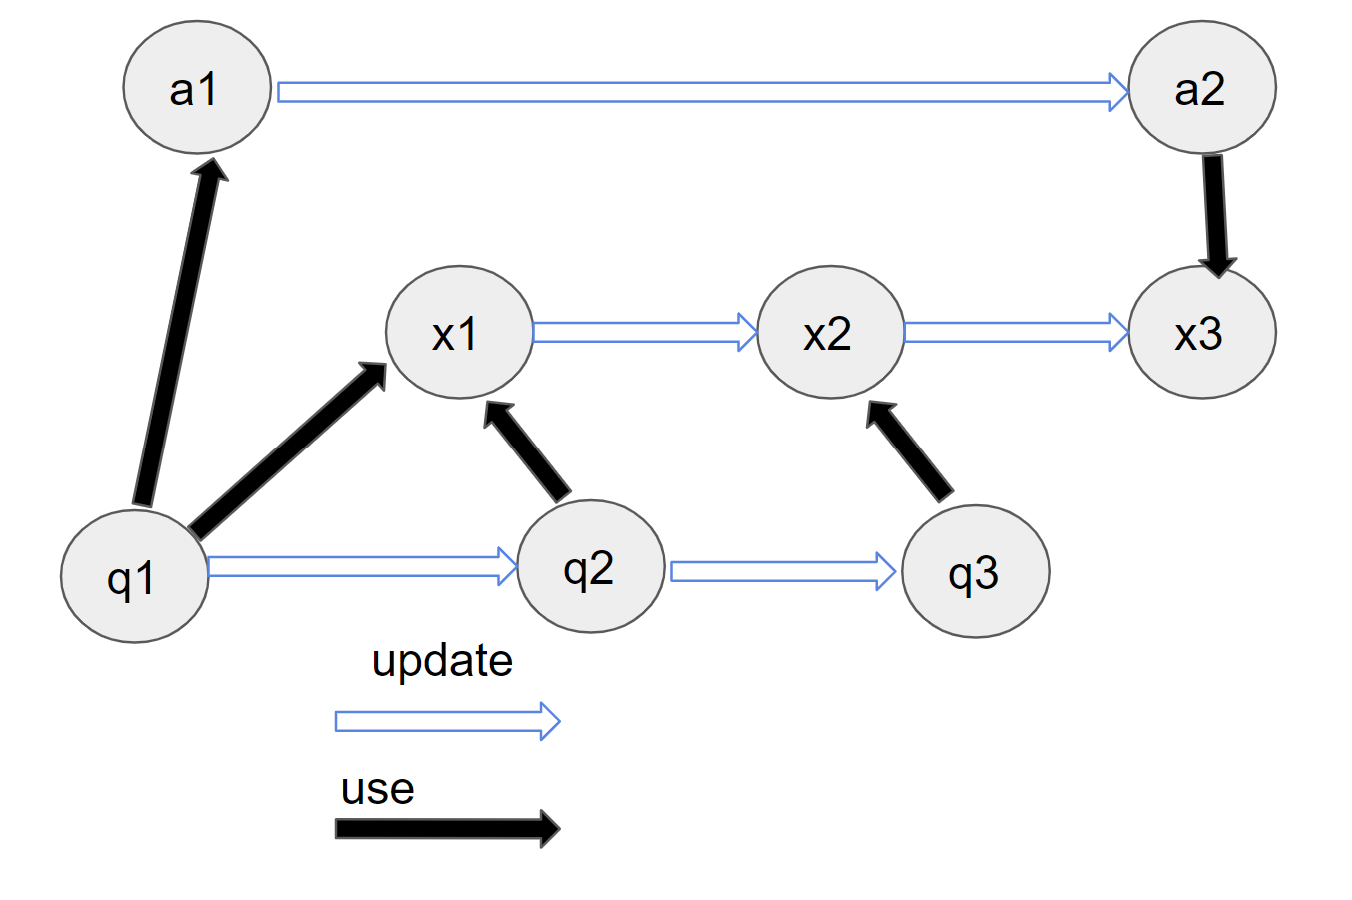
\includegraphics[width=.7\textwidth]{book/chapter-promisesandperils/pics/UniversalExample.jpg}
	\caption{Conceptual example of the Software Universe Graph, depicting the use and update relationships between different software units.}
	\label{fig:SUG}
\end{figure*}
%%%%%%%%%%%%%%%%%%%%%%%%%%%%%%%%%%%%%%%%%%%%%


\paragraph{\textbf{Component-based Representation as a Software Universe Graph}}
\label{PPM:sec:SUG}

First introduced by Kula et al.~\cite{KulaSANER18}, the \textit{Software Universe Graph} (SUG) is a structural abstraction of the software ecosystem of third-party libraries.
Figure \ref{fig:SUG} provides an illustration of the different relationships within the graph.
Let $G= (N,E)$ represent a graph $G$. $N$ is a set of nodes, each node representing a software unit. 
We define a software unit as a version instance of any software program. 

The authors then present the \textit{use} and \textit{update} relationships that exist in the ecosystem.
Hence, the edges $E$ are composed of $E_{use}$ and $E_{update}$. $E_{use}$ is a set of \textit{use-relations} and $E_{update}$ is a set of \textit{update-relations}.

\begin{definition}
An edge $u \rightarrow v \in E_{use}$ means that $u$ uses $v$. The defined functions of $E_{use}$ are:

\begin{equation}
\small
\small \use(u)\equiv \{v|u \rightarrow v\}
\normalsize
\end{equation}
\begin{equation}
\small
\small \useBy(u)\equiv \{v|v \rightarrow u\}
\normalsize
\end{equation}
\end{definition}

Use-relations can be extracted from either the source code or configuration files. 
As shown in Figure \ref{fig:SUG}, node $a1$ uses node $x1$. 
In addition, node $x1$ is used by nodes $a1$, $q1$, and $q2$. Parallel edges for node pairs are not allowed.

\begin{definition}
We represent an update relation from node $a$ to $b$ using $ a \Rightarrow b $, which means that the newer update $b$ was released from node $a$ and is defined as:
\begin{equation}
\small a \Rightarrow b \in E_{update}
\end{equation}
\end{definition}

Update relations refer to when a successive release of a software unit is made available. Figure \ref{fig:SUG} shows that node $q1$ is first updated to node $q2$. Later, node $q2$ is updated to the latest node $q3$. Hence, $q1 \Rightarrow q2 \Rightarrow q3$.
Note that an update should not be confused with forking. 
We distinguish a fork as a separate software unit. 
Each node in the SUG should be denoted by three attributes: \texttt{<name,release,time>}.  
For a node $u$, we define:

\begin{itemize}
	\item \textbf{u.name} Name is the string representation identifier of a software unit.
	We introduce the name axiom: For nodes $u$ and $v$, if $u \Rightarrow v$, then $u.name = v.name$ holds.
	
	\item \textbf{u.release}. Release refers to the specific assigned change reference for a software unit. For nodes $u$ and $v$, if $u \Rightarrow v$
	then $v$ is the immediate successor of $u$. Note that the versioning pattern may vary from project to project. 
	\item \textbf{u.time}. Time refers to the time stamp at which node $u$ was released. For nodes $u$ and $v$ of $u \Rightarrow v$, $u.time < v.time$.
\end{itemize}

\begin{figure}
	\centering
	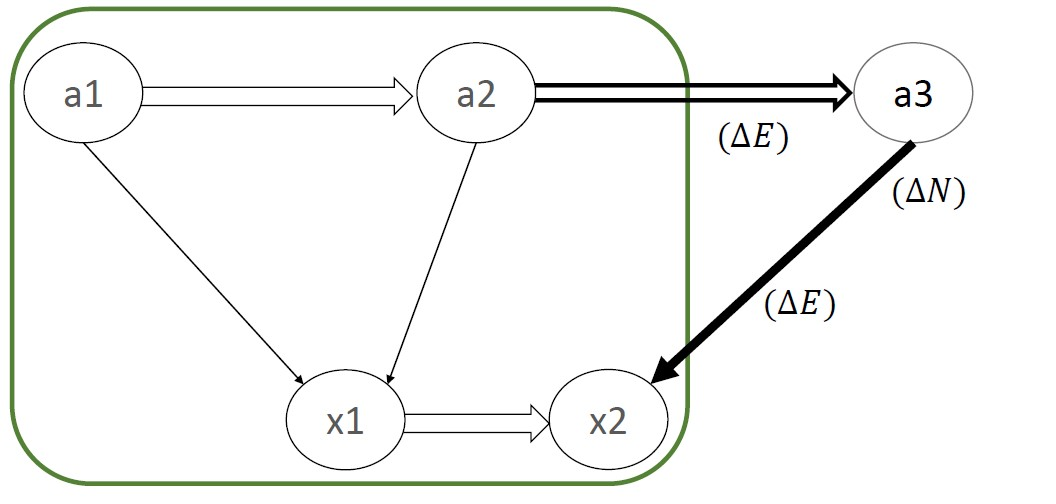
\includegraphics[width=.8\textwidth]{book/chapter-promisesandperils/pics/TemporalSUG.jpg}
	\caption{Temporal property of the SUG}
	\label{fig:SUGTemp}
\end{figure}

\begin{definition}
    
	The SUG has temporal properties.
This describes the simultaneity or ordering in reference to time. Let SUG $G = (N, E) $ be at time $t$. At time $t^{\prime} > t$, we observe an extension of $G$, such that:

\begin{equation}
\small G^{\prime} = (N \cup \Delta N, E \cup \Delta E)
\end{equation}
where $\Delta E \cap (N \times N) = \emptyset$
\end{definition}

Figure \ref{fig:SUGTemp} illustrates the temporal properties of the SUG. 
Here, it is observed that $G'$ is composed of $G$ augmented with newly added node $a3$ and its corresponding $a3 \rightarrow x2$ and $a2 \Rightarrow a3$ relations.
A SUG grows monotonically over time with only additions.
Here, we consider that modification or deletion changes on the SUG do not occur. 

\begin{definition}
    A timed SUG specifies the state of the SUG at any point in time.
So for an SUG $G=(N,E)$, we represent a timed SUG $G_{t}$ at time $t$ as a sub-graph of $G$. Formally,
\begin{equation}
\small G_t\equiv(N_{t}, E_{t})
\end{equation}
where $N_{t} = \{u|u \in N, u.time \leq t \}$ and $E_t = \{ e | e \in E \wedge e \in  N_t \}$
\end{definition}
	


\section{Data Sources}
Researchers can use various datasets to model the ecosystem using the SUG model of usage and update relationships.
The most obvious data source that has revolutionised data mining in the software engineering domain is the GitHub platform. 
Established in 2008, and then purchased by Microsoft in 2020, GitHub is home to various popular Open Source Software. 
GitHub is built on the git version control system and is useful for storing all changes made to a repository. 
In the case of the SUG, a GitHub repository can represent one software unit, whose depend relations can be extracted via a configuration file (such as the package.json file for JavaScript projects).
The repository should also contain the release information that holds the update relations.
Due to its large size, researchers and the GitHub team have made available datasets for researchers to mine, for example through the GitHub API/Graph QL.\footnote{\url{https://docs.github.com/en/graphql}} This is the backend Application Programming Interface (API) that can be used to query large amounts of data on GitHub. Most researchers use the API to download and mine information from the GitHub platform. 
It is important to note that while GitHub introduced a new feature of Dependency Graphs to map the depend relationship,\footnote{\url{https://docs.github.com/en/code-security/supply-chain-security/understanding-your-software-supply-chain/about-the-dependency-graph}} most older projects do not have this feature.
In this case, the researcher would need to manually extract and query the configuration files for dependency information. 

We refer to the first chapter for additional information on data sources for mining software ecosystems. 

\section{Promises and Perils}
\label{PPM:sec:promisesperils}

Using the SUG model of depend and use relations and the available datasets, we can now present our promises and perils of mining ecosystem information.

\subsection{Planning What Information to Mine}

\textbf{Promise 1.}\textit{
Researchers can access and link heterogeneous data related to software package ecosystems, e.g., package registries and bug trackers.}\\

When planning what information to mine from the ecosystem, researchers do not need to limit themselves to the usage and update relationship information.
Platforms that host software repositories include other software management systems such as bug trackers.
For example, GitHub allows researchers to manage GitHub Pull Requests, Issues, and Discussions not only for one project, but for multiple projects.
GitHub provides three management systems that are related to a software repository:

\begin{itemize}
    \item \textit{GitHub Discussions}\footnote{\url{https://docs.github.com/en/discussions}} - The GitHub Discussions forum is a collaborative communication forum for the community around an open source or internal project. Community members can ask and answer questions, share updates, have open-ended conversations, and follow along on decisions affecting the community's way of working.
    \item \textit{GitHub Pull Requests}\footnote{\url{https://docs.github.com/en/pull-requests}} - Pull Requests allow other developers from an ecosystem to make a contribution to a software repository. Pull requests also allow maintainers to discuss and review potential changes with collaborators and add follow-up commits before changes are merged into the software.
    \item \textit{GitHub Issues}\footnote{\url{https://docs.github.com/en/issues}} - Issues are used to track ideas, feedback, tasks, or bugs for work on GitHub.
\end{itemize}

These three systems are examples of how developers contribute to both their own and other projects. 
Hence, to incorporate this information, we can extend the SUG model, creating a model that includes a contribution relationship \cite{wattanakriengkrai2022giving}.

% Note that other platforms may also have management systems, like GitLab, BitBucket and Eclipse.

\begin{definition}
	A Dependency-Contribution graph incorporates contributions by developers whose libraries are involved in dependency relationships. 
\end{definition}

In this work \cite{wattanakriengkrai2022giving}, the authors explore the congruence between dependency updates and developer contributions, based on the original concept of social-technical congruence \cite{stcCataldo2008} where developers contribution patterns are congruent with their coordination needs. Hence, the goal is to identify contributions that are congruent to dependency updates.
As shown in Figure \ref{fig:lib} the authors extend from the typical SUG graph model where $lib_i$ depends (use) on  $lib_k$ and  $lib_j$, while  $lib_j$ also depends on $lib_k$, to the example shown in Figure \ref{fig:dc-graph}.
Different to the SUG, the graph captures developers and their contributions (i.e., the square as $dev_x$ and $dev_y$ represent two different developers making a contribution).
Here contributions are defined as $c$ (Pull Request or Issue) that were submitted to both a library and the client that depends on that library.
Hence, the graph can show contributions that are congruent to dependency changes for a software unit. 

\begin{figure}[t]
     \centering
     \begin{tikzpicture}[
         roundnode/.style={circle, fill=black, minimum size=5mm},
        squarenode/.style={fill=black, text=red, minimum size=5mm},
     ]
    \begin{scope}
         \node[roundnode, label=above:$lib_i$] (s2_proji) at (3, 2.5) {};
        \node[roundnode, label=below:$lib_j$] (s2_projj) at (4,0) {};
         \node[roundnode, label=below:$lib_k$] (s2_projk) at (2,0) {};
     \end{scope}

     \begin{scope} [every edge/.style={draw=gray, very thick}]
         \path [->] (s2_proji) edge (s2_projj);
         \path [->] (s2_proji) edge (s2_projk);
         \path [->] (s2_projj) edge (s2_projk);
     \end{scope}
     \end{tikzpicture}
    
     \caption{Example dependency graph for a given time period}
     \label{fig:lib}
     \vspace{2ex}
 \end{figure}
\begin{figure}[t]
    \centering

    \begin{tikzpicture}[
        roundnode/.style={circle, fill=black, minimum size=5mm},
        squarenode/.style={fill=black, text=red, minimum size=5mm},
    ]
    \begin{scope}
        
        \node[roundnode, label=right:$lib_i$] (s2_proji) at (4, 1.5) {};
        \node[roundnode, label=below:$lib_j$] (s2_projj) at (5,0) {};
        \node[roundnode, label=below:$lib_k$] (s2_projk) at (3,0) {};
        
        \node[squarenode, label=below:$dev_x$] (s3_devx) at (2, 3.5) {};
        
        \node[squarenode, label=below:$dev_y$] (s3_devy) at (6, 3.5) {};
        
    \end{scope}

    \begin{scope} [every edge/.style={draw=gray, very thick}]
        \path [->] (s2_proji)  edge  (s2_projj);
        \path [->] (s2_proji) edge (s2_projk);
        \path [->] (s2_projj) edge (s2_projk);
        
    \end{scope}
    \begin{scope} [every edge/.style={draw=gray, thick, double distance=2pt}]
        \path [->] (6, 2.8) edge node[left = 2mm] {$contribute$} (s2_proji);
        \path [->] (6, 2.8) edge[bend left=15] node[right = 1mm] {$contribute$} (s2_projj);
        \path [->] (2, 2.8) edge node[right = 2mm] {$$} (s2_proji);
        \path [->] (2, 2.8) edge[bend right=15] node[left = 1mm] {$contribute$} (s2_projk);
    \end{scope}
    \end{tikzpicture}
\end{figure}
\begin{figure}[t]
    \centering
    \begin{tikzpicture}[
        roundnode/.style={circle, fill=black, minimum size=5mm},
        squarenode/.style={fill=black, text=red, minimum size=5mm},
    ]
    \end{tikzpicture}
\caption{Example Dependency-Contribution graph showing relationships between contributions and dependencies}
 \label{fig:dc-graph}
\end{figure}

This is just one example of the type of research that is enabled by access to heterogeneous data related to software package ecosystems.

\smallskip\noindent\textbf{Peril 1.}\textit{
 Developers might use different identifiers when contributing to different parts of a software package ecosystem, e.g., when contributing to different libraries.}\\
 
When modelling using such graphs, there is a threat that contributors may use multiple identifiers (i.e., $c_x$ and $c_y$ are the same contributor).
This is a well-known research problem, and there has been work to merge these accounts, such as \cite{wiese2016mailing}.
GitHub has introduced mechanisms such as two-factor authentication\footnote{\url{https://docs.github.com/en/authentication/securing-your-account-with-two-factor-authentication-2fa/configuring-two-factor-authentication}} to counteract the issue of multiple identifiers.
This is since developers might be less likely to switch accounts if it requires cumbersome authentication.


\smallskip\noindent\textbf{Peril 2.}\textit{
Developers' contributions to software package ecosystems might be interspersed with bot contributions, e.g., automated dependency updates.}\\

The rise of automation and artificial intelligence has led to much work on the integration of automated scheduling (i.e., bots) into software development workflows \cite{Storey2016, Farooq2016, Wessel2018, Erlenhov2019, bot_modify_wf} to name a few. These bots are designed to perform specific tasks within a software package ecosystem. For example, a bot may be programmed to automatically update dependencies, test code changes, or deploy software to production. As an example, the Google APIs repo-automation-bots project lists bots for automated labelling of issues and pull requests, automated approval of pull requests, and triggering releases.\footnote{\url{https://github.com/googleapis/repo-automation-bots}}
Bots perform common maintenance tasks in many software projects and are now commonplace \cite{Beschastnikh2017, Urli2018,BIMAN,bot_or_not}.
Especially with bots such as dependabot (automated pull requests to update configurations to reduce the risk of vulnerability threats),\footnote{\url{https://github.com/dependabot}} more and more automation has caused a lot of noise in the contributions between projects.
There are also bots for communication and documentation \cite{Urli2018, Lin2016, Lebeuf2017a}.

To be able to draw accurate conclusions about what humans are doing in software package ecosystems, researchers should consider distinguishing between bot and human contributions.
It is also important to differentiate this from other contributions \cite{maeprasart2022understanding}.
The research community has responded well, with a wide range of techniques and tools to mitigate this peril \cite{Bodegha2021, golzadeh2022accuracy}.

\smallskip\noindent\textbf{Peril 3.}\textit{
Not all developer activities in software package ecosystems are accessible to the public, e.g., library use in proprietary settings.
}\\

Not all developer activities in software package ecosystems are accessible to the public, e.g., when the boundary between open source and industry is blurred \cite{stol2014inner}, which presents a challenge for researchers who aim to study the development process. This is particularly true in proprietary settings where software development is performed behind closed doors or is open source for a limited time period, thus resulting in the artefacts not permanently being publicly available.
This can make it difficult to understand the broader ecosystem in which a software project is developed.
Proprietary settings may lead to non-standardisation in software development practises. Different software projects may use different management systems and tools, making it difficult to accurately compare and analyse software development activities across various projects. For example, some projects may use communication, documentation, and other management tools not captured on the same platform \cite{montgomery2022alternative}. For example, some projects might use Bugzilla instead of issues and pull requests for their bug and code review systems, while others may use Discord, Slack channels, or email threads for their communication needs.

This lack of standardisation in software development practises presents a challenge for researchers who study the software package ecosystem and understand the development process. To address this issue, researchers should strive to collect data from a diverse set of projects to gain a comprehensive understanding of the software package ecosystem. In addition, researchers may need to adjust their methodologies or data collection techniques to accommodate the different tools and practises used by different software projects.

\subsection{Defining Components and their Dependencies}

\smallskip\noindent\textbf{Promise 2.}\textit{
Researchers can access a software package ecosystem's dependency network through package managers and registries, e.g., npm lists the dependencies and dependents for over a million libraries.}\\


With the rise of curated datasets like libraries.io, researchers can now recover and model dependency relations between software units using pre-extracted datasets.
Table \ref{tab:PM_features} shows examples of popular package managers mined from the libraries.io dataset in 2020. 

\begin{table*}[]
\caption{Summary of 13 package managers from libraries.io as ranked by TIOBE in 2020}
 \label{tab:PM_features}
 \centering
\begin{tabular}{@{}llrlll@{}}
\toprule
\begin{tabular}[c]{@{}l@{}}Package \\ Ecosystem\end{tabular} & \begin{tabular}[c]{@{}l@{}}Programming \\ Language\end{tabular} &  \begin{tabular}[c]{@{}l@{}}Tiobe \\ Rank\end{tabular} & Environment & \begin{tabular}[c]{@{}l@{}}Dependency \\ Tree\end{tabular} & \begin{tabular}[c]{@{}l@{}}Package   \\Archive link\end{tabular}\\ \midrule
PyPI & Python & 2 & Python & Flat & pypi.org  \\
Maven & Java & 3 & JVM & Flat & Maven.org  \\
Bower & JavaScript & 7 & Node.js & Flat & bower.io  \\
Meteor & JavaScript & 7 & Node.js & Nested & atmospherejs.com \\
npm & JavaScript & 7 & Node.js & Nested (v2) & npmjs.com  \\
Packagist & PHP & 8 & PHP & Flat & packagist.org \\
Puppet & Ruby & 13 & Ruby MRI & Flat & forge.puppet.com  \\
RubyGems & Ruby & 13 & Ruby MRI & Flat & rubygems.org  \\
CRAN & R & 14 & RStudio & Flat & cran.r-project.org  \\
CPAN & Perl & 15 & Perl & Flat & metacpan.org  \\
GO & Golang & 20 & Go & Flat & pkg.go.dev  \\
NuGet & C\#, VB & 5, 6 & .NET & Flat & nuget.org \\
Anaconda & Python, R, C\# & 2, 14, 5 & Anaconda & Flat & anaconda.org  \\ \bottomrule
\end{tabular}
\end{table*}

\smallskip\noindent\textbf{Peril 4.}\textit{
Different software package ecosystems define the concept of ``dependency'' differently, e.g., by allowing or not allowing different versions of a library on the same dependency tree.
}\\

Different software package ecosystems have varying definitions of what constitutes a dependency. For example, some ecosystems may allow multiple versions of a library to exist on the same dependency tree, while others may restrict developers to a single version of a library \cite{Islam}. These restrictions are often based on the programming language being used, as different languages have different approaches to managing dependencies. It is important to consider the restrictions on dependency relationships when studying software package ecosystems, as they can have a major impact on the development process. For example, the ability to use multiple versions of a library on the same dependency tree can greatly simplify the process of updating dependencies and can make it easier to resolve conflicts between libraries.

One way to visualise the impact of these restrictions is to compare the difference between a nested dependency tree and a directed dependency tree, as shown in Figure \ref{fig:nest}.\footnote{Taken from \url{https://npm.github.io/how-npm-works-docs/npm3/how-npm3-works.html}} This distinction is important because it highlights the different ways that a software unit can depend on different versions of the same library.
In this example, npm v3 creates the dependency tree based on the installation order, therefore flattening unnecessary nested dependencies (i.e., B v1.0 in cyan). This reduces the complexity of a nested tree by resolving some of the transitive dependencies (nested dependencies).

\begin{figure}
	\centering
	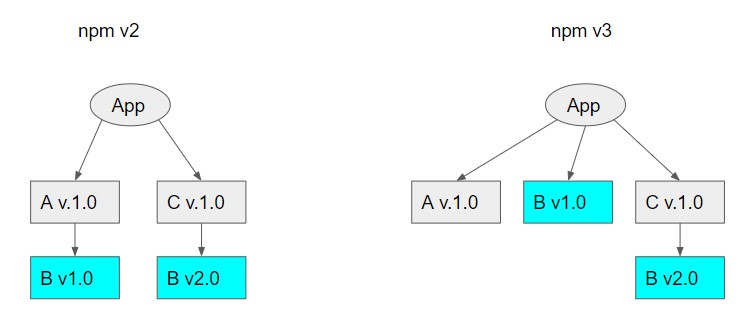
\includegraphics[width=.8\textwidth]{book/chapter-promisesandperils/pics/nestedv2.jpg}
	\caption{Difference between flat and nested dependencies}
	\label{fig:nest}
\end{figure}

\smallskip\noindent\textbf{Peril 5.}\textit{
Developers might declare a dependency to other parts of a software package ecosystem but not use it, e.g., because they failed to update its removal.
}\\

It is common for developers to declare dependencies on other parts of the software package ecosystem but not always use them. This can happen for various reasons, such as forgetting to remove the dependency after it is no longer needed. This can pose a challenge for researchers who are trying to extract dependencies from package managers, like those in configuration files, as there may be inconsistencies between the listed dependencies and what is actually being compiled and used by the code. This can lead to a biased understanding of the software package ecosystem and the relationships between software components.

To address this issue, there have been numerous efforts to track the actual library dependencies compiled and executed in software systems. These efforts aim to provide a more accurate understanding of the dependencies and the relationships between software components. For example, research has been conducted on the use of dynamic analysis to track compiled dependencies in real time and on the development of tools to automatically detect and track executed dependencies \cite{Zapata:ICSME2018, Ponta2018,Chinthanet:ASE2020}.

\subsection{Defining Boundaries and Completeness}

\smallskip\noindent\textbf{Promise 3.}\textit{
Researchers can use the boundaries of software package ecosystems to study communities of developers, e.g., developers contributing to and/or benefiting from the npm ecosystem.
}\\

Following Promise 2, the emergence of package managers has also led to studies that approximate software communities.
Using the libraries.io dataset, researchers were able to study projects that host libraries that use package managers.
Researchers have used this dataset to compare different library ecosystems \cite{kikas.2017,decan:emse:2019,CogoDown2019}.


\smallskip\noindent\textbf{Peril 6.}\textit{
Package managers do not always represent software package ecosystems, their communities, or their sub-communities, e.g., in cases where multiple package managers exist.
}\\

Package managers are a fundamental aspect of software package ecosystems, but do not always fully represent the complex relationships and interactions that occur within a community of developers and users, as shown in Table~\ref{tab:PM_features}. In some cases, multiple package managers exist for the same programming language, creating a complex landscape of software libraries and dependencies that are not always easily understood. For instance, Bower and Meteor manage npm libraries, which can lead to confusion and overlap in the management of dependencies.

Similarly, Java, Scala, Android, and other Java-based open source communities all use the Maven package manager, but each of these communities has its own unique set of libraries, dependencies, and development practises. Researchers should be aware of the limitations of package managers when studying software package ecosystems, and consider the broader context and relationships that exist within these communities. 

\smallskip\noindent\textbf{Peril 7.}\textit{
Lack of activity in parts of a software package ecosystem does not necessarily indicate project failure, e.g., when highly depended-upon libraries are feature-complete.
}\\

It is important to note that lack of activity in a part of a software package ecosystem does not always mean project failure \cite{coelho2017modern}. In some cases, highly relied-upon libraries that have reached feature-completeness may see little activity, but continue to be used by the software community. 

However, it is still important to consider the long-term sustainability of these libraries, especially given the rate at which technology and software development practises change. This has become a topic of interest in recent years, and researchers have explored best practises for sustaining open source projects and ensuring their continued success \cite{Ait2022,valiev2018ecosystem}. Understanding the factors that contribute to project sustainability is important to ensure the longevity and continued growth of software package ecosystems.

\smallskip\noindent\textbf{Peril 8.}\textit{
Sampling from a software package ecosystem is challenging since sub-setting might alter the dependency network, e.g., by breaking dependency chains.
}\\

Sampling from a package ecosystem is not straightforward, as the sample composition can be significantly affected due to missing dependency links between libraries. For instance, a subset of the ecosystem might alter the dependencies between libraries, leading to the breakdown of the dependency chains. This could lead to an incomplete picture of the software package ecosystem, leading to incorrect conclusions from a study. To minimise this risk, researchers should carefully consider the boundaries of their study and choose the appropriate sampling method based on the research questions and goals. For example, researchers could focus on popular, highly dependent, or risk-vulnerable aspects of the ecosystem as a starting point. 
For some ecosystems, the number of downloads, GitHub stars, and watchers are other aspects for the researcher to utilise.


\smallskip\noindent\textbf{Peril 9.}\textit{
Sampling from a software package ecosystem is challenging since the dependency network changes over time, e.g., when dependencies are added, removed, upgraded, or downgraded.
}\\

The dynamic nature of package ecosystems and the constant changes to their dependencies can impact the generalisability of the results. Therefore, it is important to also consider the time granularity of the analysis. For example, if the goal is to understand the evolution of dependencies over time, a finer time granularity may be necessary to capture the smaller changes and trends. However, if the goal is to understand the overall structure and relationships within the ecosystem, a coarser time granularity may be sufficient. Based on recent studies \cite{wattanakriengkrai2022giving,valiev2018ecosystem,Mirsaeedi:icse2020, Brindescu:emse2020, Nassif:icsme2017}, a three-month window seems appropriate for some studies.
Another level of granularity to consider is the size of the component. For instance, there are cases where a single package may contain more than one repository, especially for large library frameworks. 
The granularity also depends on the nature of the ecosystem itself. For instance, researchers should understand whether the ecosystem comprises library packages (e.g., PyPI), plugins (e.g., Eclipse), or is a library distribution (e.g., Android).



\subsection{Analysing and Visualising the Data}

\textbf{Peril 10.}\textit{
Analysing and visualising entire software package ecosystems is challenging due to their size, e.g., in terms of nodes and edges in the network.
}\\

The size of software package ecosystems implies large data sets, which can be overwhelming for tools and algorithms to analyse and display. Therefore, it may be necessary to make choices about the granularity of the data included in the analysis and visualisation. Another alternative is to focus on the most critical parts of the software package ecosystem, such as the high-level structure, highly dependent packages, or parts of the system that pose a risk to security and reliability. 
The key is to strike a balance between detail and simplicity, providing a meaningful representation of the ecosystem while being able to handle the complexity of its size.


\section{Application: When to Apply Which Peril}
\label{PPM:sec:application}

We include a disclaimer stating that not all perils are applicable to every mining situation. To demonstrate the practical application of our perils and their mitigation, we present two case studies that involve mining the software package ecosystem. Each case study has a distinct research objective and focusses on a specific dataset to be mined.

\subsection{Two Case Studies}
Table \ref{tab:cases} presents the two case studies we have selected for this analysis.
The \textit{first case} involves mining for contributions congruent to dependency updates \cite{wattanakriengkrai2022giving}. 
In this work, the authors mine GitHub repositories for Pull Requests and Issues that were submitted and merged congruent to dependency updates within the npm ecosystem. 
The \textit{second case} involves mining communication data for the Eclipse ecosystem \cite{Nugroho2021}. Although the second case does not mine for dependency relations (i.e., use relations),  we show that these perils still apply when mining for other relationships in an ecosystem.
Moreover, the second case studies the Eclipse ecosystem, which is a different dataset compared to the more popular GitHub dataset.

\subsection{Applying Perils and their Mitigation Strategies}
Table \ref{tab:perilsapp} provides a summary of the perils that can be applied to each of the case studies. We will now go into the details of mitigation strategies based on these perils. 
For better organisation and understanding, we have grouped the perils according to the four logical processes for mining.

\smallskip\noindent\textbf{Information to Mine}. 
The first set of mitigation strategies, which addresses perils 1-3, focusses on planning which information to mine. There are two primary strategies that researchers can employ:


\begin{enumerate}
    \item Researchers should use research tools and techniques to remove noise and other biases in the dataset, such as bot detection and the handling of multiple identities. This strategy was implemented in both case studies, as contributions and discussions often have the potential to involve bots or developers with multiple identities.
\item Depending on the research goals, researchers should recognise that not all contributions are equal and filter the dataset accordingly.
\end{enumerate}

We applied these two strategies to both cases. In the first case, the goal was to capture all congruent contributions, so we filtered out contributions made to libraries without dependencies. Since all npm packages are listed in the registry, Peril 3 (private activities) did not apply.
In the second case, we addressed Peril 1 by conducting a qualitative analysis to ensure that the member identities were not duplicated, as Eclipse developers were known to change identities. To mitigate Peril 2, we removed bot responses. For the second case, since all forum data is made public, Peril 3 did not apply.


\begin{table}
\centering
\caption{Description of the research objectives and datasets for the case studies}
 \label{tab:cases}
\begin{tabular}{lp{5cm}r} 
\toprule
\textbf{Case Study} & \textbf{Research Objective}                                                          & \textbf{Datasets}           \\
\midrule
Wattanakriengkrai \etal \cite{wattanakriengkrai2022giving}             & Explore code contributions between library and client (i.e, use-relations)  & libraries.io\\
& &  GitHub API \\
Nugroho \etal \cite{Nugroho2021}                & Explore discussion contributions between contributors (i.e., contributions) & Eclipse API                \\
\bottomrule
\end{tabular}
\end{table}

\begin{table}
\centering
\caption{Application of each peril to the case studies}
 \label{tab:perilsapp}
\begin{tabular}{rp{8cm}ccc} 
\toprule                   
& \textbf{Perils}       & case 1      & case 2                 \\
                                                                               & & npm  & Eclipse   \\
\midrule
\textbf{P1} &Developers might use different identifiers when contributing to different parts of a software package ecosystem, e.g., when contributing to different libraries.                             &    \CheckedBox         &          \CheckedBox           \\ 
%\hline
\textbf{P2} & Developers' contributions to software package ecosystems might be interspersed with bot contributions, e.g., automated dependency updates.                                                      &      \CheckedBox               &      \CheckedBox               \\ 
%\hline
\textbf{P3} & Not all developer activities in software package ecosystems are accessible to the public, e.g., library use in proprietary settings.                                                         &         -           &      \CheckedBox               \\ 
%\hline
\textbf{P4} & Different software package ecosystems define the concept of \`{}\`{}dependency'' differently, e.g., by allowing or not allowing different versions of a library on the same dependency tree. &         \CheckedBox       &     -                            \\ 
%\hline
\textbf{P5} & Developers might declare a dependency to other parts of a software package ecosystem but not use it, e.g., because they failed to update its removal.                                        &     -           &  -    \\
%\hline
\textbf{P6} &Package managers do not always represent software package ecosystems, their communities, or their sub-communities, e.g., in cases where multiple package managers exist.                     &     -                   &  -                  \\
%\hline
\textbf{P7} & Lack of activity in parts of a software package ecosystem does not necessarily indicate project failure, e.g., when highly depended-upon libraries are feature-complete.                     &       \CheckedBox         &  -                           \\
%\hline
\textbf{P8} &Sampling from a software package ecosystem is challenging since sub-setting might alter the dependency network, e.g., by breaking dependency chains.                                         &        \CheckedBox        &     \CheckedBox                                \\
%\hline
\textbf{P9} &Sampling from a software package ecosystem is challenging since the dependency network changes over time, e.g., when dependencies are added, removed, upgraded, or downgraded.               &       \CheckedBox         &     -                          \\
%\hline
\textbf{P10} &Analysing and visualising entire software package ecosystems is challenging due to their size, e.g., in terms of nodes and edges in the network.                                  &        \CheckedBox      &      \CheckedBox               \\
\bottomrule
\end{tabular}
\end{table}

\smallskip\noindent\textbf{Defining Dependencies}. 
The second set of perils (Perils 4-5) is related to dependency relationships between software units, and only the first case study is applicable. To address these perils, researchers should adopt the following strategy:

\begin{enumerate}
    \item Researchers should not rely solely on listed dependencies in configuration files (e.g., pom.xml, package.json, etc.) as a measure of dependency between two components. Instead, code-centric approaches should be used to validate which libraries are actually depended upon.
\end{enumerate}

For example, in the first case, in addition to mining the configuration information, the authors also analysed the similarity of the source code contributions to address Peril 4. Regarding Peril 5, since the study's objective was to investigate changes to the configuration files, the risk of the update not being executed was deemed less important.
It is important to note that the second case study did not include dependency analysis and, therefore, these perils did not apply.

\begin{figure*}[]
    \centering
    \begin{subfigure}{0.9\linewidth}
         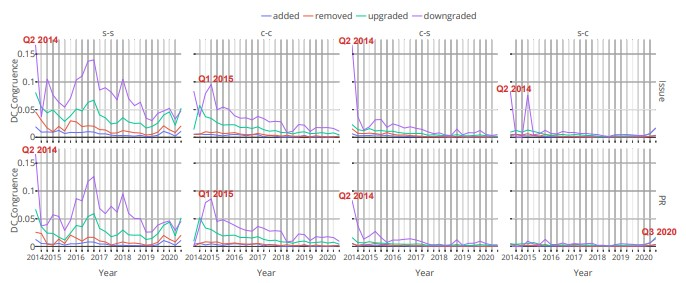
\includegraphics[width=1.1\textwidth]{book/chapter-promisesandperils/pics/congruentViz.jpg}
         \caption{Visualization of a Time analysis for 107,242 libraries.}
     \end{subfigure}
     \begin{subfigure}{0.9\linewidth}
         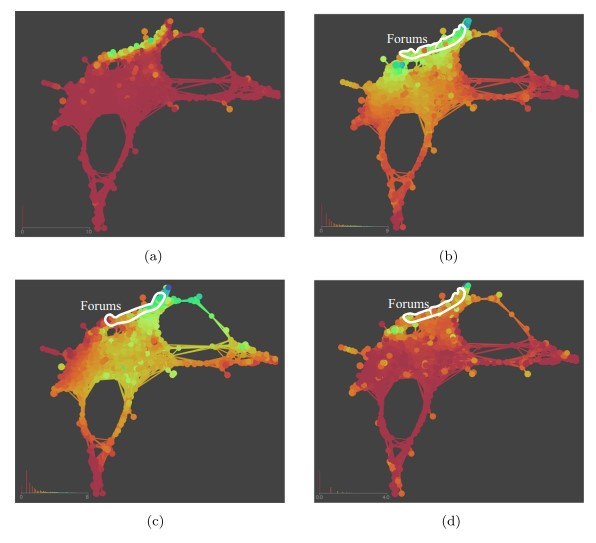
\includegraphics[width=1\textwidth]{book/chapter-promisesandperils/pics/eclipseViz.jpg}
         \caption{A Visual Topology map for 832,058 threads}
     \end{subfigure}
    \caption{Visualisation examples for the two case studies}
    \label{fig:visCase}
\end{figure*}

\smallskip\noindent\textbf{Defining Boundaries}.
The third set of perils (Perils 6-9) is related to the definition of boundaries and completeness and is relevant for both case studies. To mitigate these perils, we recommend the following strategies:

\begin{enumerate}
    \item Researchers should recognise that a dormant project does not necessarily mean that it is inactive. Instead, studies can use alternative heuristics, such as the number of dependents and dependencies, as better indicators of a project's importance in the ecosystem.
    \item Researchers should not rely solely on the programming language to define sub-communities. Using a common package manager for the programming language is a more effective rule of thumb for distinguishing boundaries.
    \item Researchers should avoid random sampling. Instead, sampling should be tailored to the research goals by considering factors such as an appropriate time window or focussing on specific attributes of components (e.g., most dependents, most popular, most contributors).
\end{enumerate}


Peril 6 did not apply to any of the case studies. 
Particularly for the first case, since the goal was to explore the npm package ecosystem, we assumed that the boundaries were clearly defined by the npm registry. 
Similarly, the second case study used the generic Eclipse platform as the boundary. 
Peril 7 was applied to the npm study, while Peril 8 was applied to both case studies. 
As a result, the two cases conducted a qualitative analysis of the dataset to gain deeper insights.
In the first case study, a three-month time window was created to capture dependencies. 
For the second case study, forum contributors were sampled into three groups (i.e., junior, member, or senior) according to the sliding window of their contributions. 

\smallskip\noindent\textbf{Visualisation}.
The final peril (Peril 10) relates to visualisation, which can be challenging due to the vast size and complexity of software ecosystems. As it is not feasible to visualise every aspect of an ecosystem simultaneously, a focused approach is necessary. A mitigation strategy is to select specific attributes of the ecosystem (e.g., the most dependent, most popular, and most contributions) that align with the research needs and objectives. 

Figure \ref{fig:visCase} shows two cases where visualizations are employed to gain insights, especially for large datasets.
In the first figure (a), we visualize the distributions of the data set and applied the appropriate statistical tests, along with the effect size, to test our hypotheses and answer research questions. 
In the second example (b), although not directly related to package ecosystems, the authors utilized a topological visualization \cite{Lum2013ExtractingIF} to gain insights on the over 800,000 forum threads of discussions. 



\section{Chapter Summary}
In this chapter, we explore the various aspects of mining information from the software package ecosystem, presenting three promises and ten perils that researchers should be aware of when undertaking such tasks. The chapter is structured around four key processes for mining: 1) Planning what Information to Mine, 2) Defining Components and their Dependencies, 3) Defining Boundaries and Completeness, and 4) Analysing and Visualising the Data. To help new and experienced researchers navigate these challenges, we introduced the SUG model, which can serve as a valuable tool to minimise threats to validity. Although some perils may be more relevant to specific research objectives, our aim is to equip researchers with the knowledge and resources needed to confidently gather and integrate software package ecosystem data into their work.

% %Semantic labeling three-letter-code: FRK (e.g. \chapter{FRK})

% 
\title{Promises and Perils of Mining \\ Software Package Ecosystem Data}
\author{Raula Gaikovina Kula \and Katsuro Inoue \and Christoph Treude}
\institute{Raula Gaikovina Kula \at Nara Institute of Science and Technology, Japan, \email{raula-k@naist.jp}
\and Katsuro Inoue \at Nanzan University, Japan \email{ inoue599@nanzan-u.ac.jp}
\and  Christoph Treude \at The University of Melbourne, Australia \email{christoph.treude@unimelb.edu.au}}

\maketitle
\label{PPM:ch}
\abstract*{The use of third-party packages is becoming increasingly popular and has led to the emergence of large software package ecosystems with a maze of inter-dependencies. Since the reliance on these ecosystems enables developers to reduce development effort and increase productivity, it has attracted the interest of researchers: understanding the infrastructure and dynamics of package ecosystems has given rise to approaches for better code reuse, automated updates, and the avoidance of vulnerabilities, to name a few examples. But the reality of these ecosystems also poses challenges to software engineering researchers, such as: How do we obtain the complete network of dependencies along with the corresponding versioning information? What are the boundaries of these package ecosystem? How do we consistently detect dependencies that are declared but not used? How do we consistently identify developers within a package ecosystem? How much of the ecosystem do we need to understand to analyse a single component? How well do our approaches generalise across different programming languages and package ecosystems? In this chapter, we review promises and perils of mining the rich data related to software package ecosystems available to software engineering researchers.}

\abstract{The use of third-party packages is becoming increasingly popular and has led to the emergence of large software package ecosystems with a maze of inter-dependencies. Since the reliance on these ecosystems enables developers to reduce development effort and increase productivity, it has attracted the interest of researchers: understanding the infrastructure and dynamics of package ecosystems has given rise to approaches for better code reuse, automated updates, and the avoidance of vulnerabilities, to name a few examples. But the reality of these ecosystems also poses challenges to software engineering researchers, such as: How do we obtain the complete network of dependencies along with the corresponding versioning information? What are the boundaries of these package ecosystems? How do we consistently detect dependencies that are declared but not used? How do we consistently identify developers within a package ecosystem? How much of the ecosystem do we need to understand to analyse a single component? How well do our approaches generalise across different programming languages and package ecosystems? In this chapter, we review promises and perils of mining the rich data related to software package ecosystems available to software engineering researchers.}

%%%%%%%%%%%%%%%%%%%%%%%%%%%%%%%%%%%%%%%%%%%%%%%%%%%%%%%%%%%%%%%%%%

\section{Introduction}
\label{PPM:sec:definition}

Third-party libraries are a great way for developers to incorporate code without having to write their own for every functionality required. By using these libraries, developers can save time and energy while still getting the functions they need.
Using third-party libraries is becoming increasingly popular and has led to the emergence of large software package ecosystems such as npm. While these ecosystems offer many benefits, they also come with risks, such as software vulnerability attacks \cite{Chinthanet:ASE2020}.

Large software package ecosystems are a treasure trove for researchers who can investigate a wide range of questions. For example, by studying activity in large ecosystems, researchers can identify which libraries are the most popular and learn what characteristics make them successful \cite{kikas.2017,decan:emse:2019}.
Additionally, research on large ecosystems can help developers understand how to protect their code from malicious actors who may attempt to exploit vulnerabilities or insert malware into popular libraries.
Studying large software package ecosystems can help us better understand the dynamics of open source development in general. Open source development is a complex process that involves many different stakeholders working together (or sometimes competing) to create valuable code that anyone can use or improve upon. By understanding how these interactions play out in different types of ecosystem structures -- including those with many small projects versus few very large ones -- we can develop insights that might be applicable more broadly across other types of collaborative systems.

In this chapter, we identify and discuss promises and perils during the mining process, ranging from planning what information to mine from the ecosystem to analysing and visualising the mined data. 
Therefore, the chapter is broken down into these logical processes of mining ecosystem data: 1) Planning what Information to Mine, 2) Defining Components and their Dependencies, 3) Defining Boundaries and Completeness, and 4) Analysing and Visualising the Data.

This chapter is intended for researchers and practitioners who are interested in exploring and exploiting software package ecosystem information from a diverse range of sources that are publicly available. 
We also highlight the pitfalls to consider during the mining process, particularly when these pitfalls could lead to a misinterpretation of the analysis and results. 
The chapter is written in a manner that encourages newcomers who have little or no experience or who are interested in utilising ecosystem data across different disciplines outside of software engineering.
Our goal is to get new researchers quickly accustomed to gathering ecosystem information for their research.


\section{A Component-based Software Ecosystem}

Defined as a component-based software ecosystem, we suggest using the term `software package ecosystem' as a suitable term for the symbiotic relationships among third-party library components (as software projects or repositories), as these libraries and their dependent clients coexist on the same technological platform, therefore sharing the same environment and other internal and external factors (e.g., security threats, sharing contributions, etc.).
Please refer to the Introduction chapter for an in-depth definition of the different types of software ecosystems.
We present our interpretation of the software package ecosystem in Kula et al.~\cite{KulaSANER18}, where we formally define a package ecosystem using a Software Universe Graph (SUG).
This is modelled as a structured abstraction of the evolution of software systems and their library dependencies over time.

%%%%%%%%%%%%%%%%%%%%%%%%%%%%%%%%%%%%%%%%%%
\begin{figure*}
	\centering
	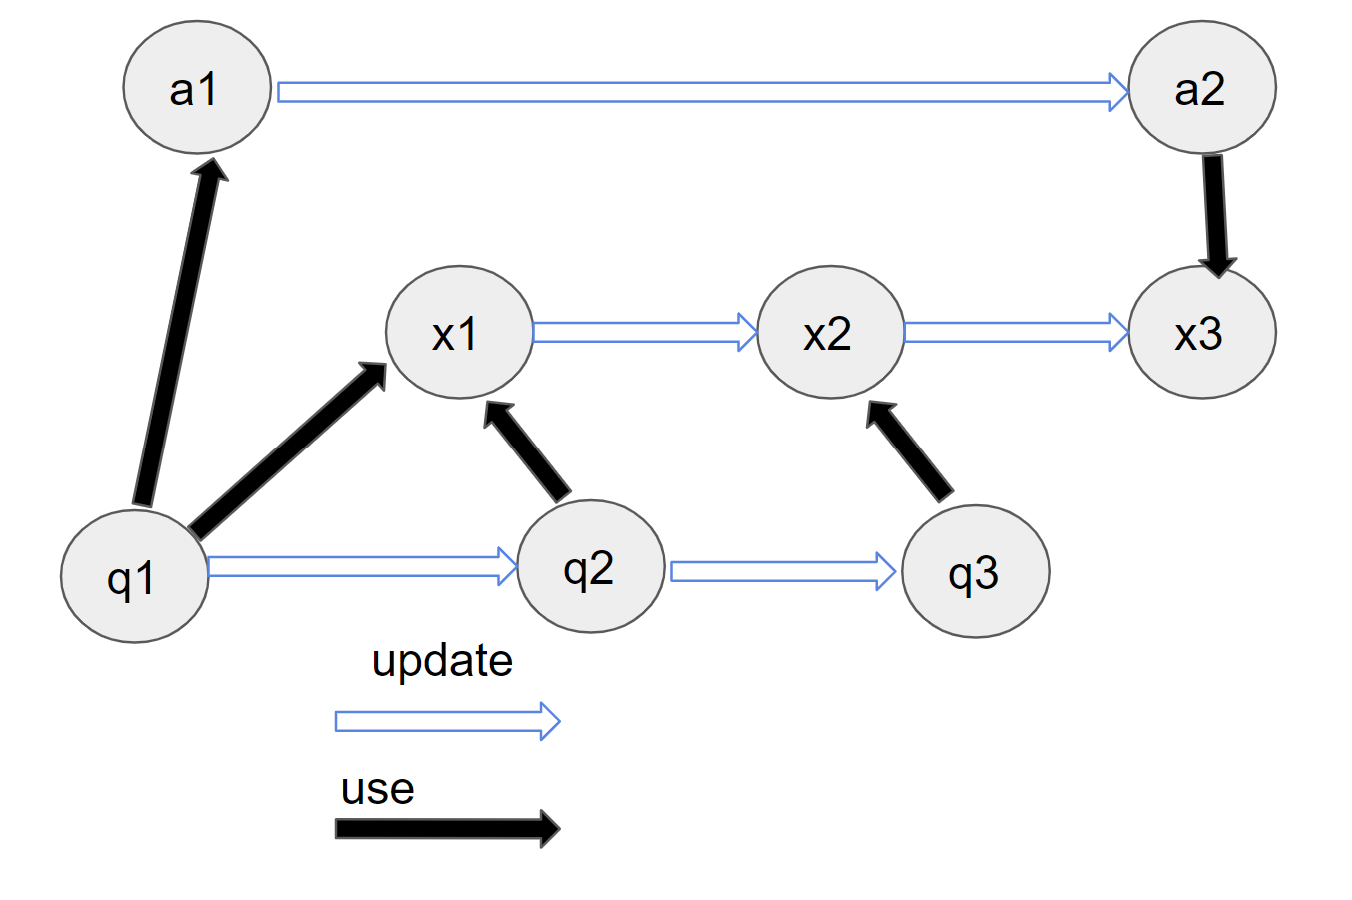
\includegraphics[width=.7\textwidth]{book/chapter-promisesandperils/pics/UniversalExample.jpg}
	\caption{Conceptual example of the Software Universe Graph, depicting the use and update relationships between different software units.}
	\label{fig:SUG}
\end{figure*}
%%%%%%%%%%%%%%%%%%%%%%%%%%%%%%%%%%%%%%%%%%%%%


\paragraph{\textbf{Component-based Representation as a Software Universe Graph}}
\label{PPM:sec:SUG}

First introduced by Kula et al.~\cite{KulaSANER18}, the \textit{Software Universe Graph} (SUG) is a structural abstraction of the software ecosystem of third-party libraries.
Figure \ref{fig:SUG} provides an illustration of the different relationships within the graph.
Let $G= (N,E)$ represent a graph $G$. $N$ is a set of nodes, each node representing a software unit. 
We define a software unit as a version instance of any software program. 

The authors then present the \textit{use} and \textit{update} relationships that exist in the ecosystem.
Hence, the edges $E$ are composed of $E_{use}$ and $E_{update}$. $E_{use}$ is a set of \textit{use-relations} and $E_{update}$ is a set of \textit{update-relations}.

\begin{definition}
An edge $u \rightarrow v \in E_{use}$ means that $u$ uses $v$. The defined functions of $E_{use}$ are:

\begin{equation}
\small
\small \use(u)\equiv \{v|u \rightarrow v\}
\normalsize
\end{equation}
\begin{equation}
\small
\small \useBy(u)\equiv \{v|v \rightarrow u\}
\normalsize
\end{equation}
\end{definition}

Use-relations can be extracted from either the source code or configuration files. 
As shown in Figure \ref{fig:SUG}, node $a1$ uses node $x1$. 
In addition, node $x1$ is used by nodes $a1$, $q1$, and $q2$. Parallel edges for node pairs are not allowed.

\begin{definition}
We represent an update relation from node $a$ to $b$ using $ a \Rightarrow b $, which means that the newer update $b$ was released from node $a$ and is defined as:
\begin{equation}
\small a \Rightarrow b \in E_{update}
\end{equation}
\end{definition}

Update relations refer to when a successive release of a software unit is made available. Figure \ref{fig:SUG} shows that node $q1$ is first updated to node $q2$. Later, node $q2$ is updated to the latest node $q3$. Hence, $q1 \Rightarrow q2 \Rightarrow q3$.
Note that an update should not be confused with forking. 
We distinguish a fork as a separate software unit. 
Each node in the SUG should be denoted by three attributes: \texttt{<name,release,time>}.  
For a node $u$, we define:

\begin{itemize}
	\item \textbf{u.name} Name is the string representation identifier of a software unit.
	We introduce the name axiom: For nodes $u$ and $v$, if $u \Rightarrow v$, then $u.name = v.name$ holds.
	
	\item \textbf{u.release}. Release refers to the specific assigned change reference for a software unit. For nodes $u$ and $v$, if $u \Rightarrow v$
	then $v$ is the immediate successor of $u$. Note that the versioning pattern may vary from project to project. 
	\item \textbf{u.time}. Time refers to the time stamp at which node $u$ was released. For nodes $u$ and $v$ of $u \Rightarrow v$, $u.time < v.time$.
\end{itemize}

\begin{figure}
	\centering
	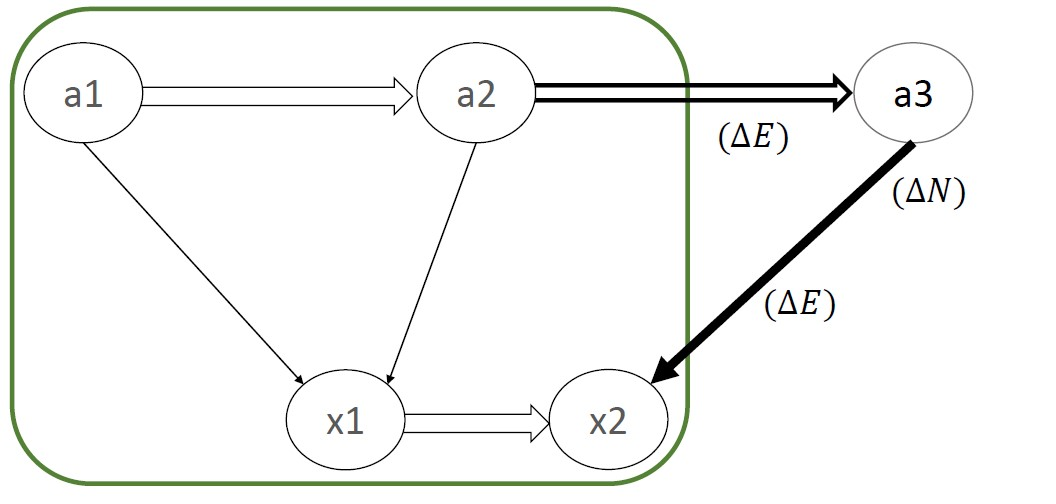
\includegraphics[width=.8\textwidth]{book/chapter-promisesandperils/pics/TemporalSUG.jpg}
	\caption{Temporal property of the SUG}
	\label{fig:SUGTemp}
\end{figure}

\begin{definition}
    
	The SUG has temporal properties.
This describes the simultaneity or ordering in reference to time. Let SUG $G = (N, E) $ be at time $t$. At time $t^{\prime} > t$, we observe an extension of $G$, such that:

\begin{equation}
\small G^{\prime} = (N \cup \Delta N, E \cup \Delta E)
\end{equation}
where $\Delta E \cap (N \times N) = \emptyset$
\end{definition}

Figure \ref{fig:SUGTemp} illustrates the temporal properties of the SUG. 
Here, it is observed that $G'$ is composed of $G$ augmented with newly added node $a3$ and its corresponding $a3 \rightarrow x2$ and $a2 \Rightarrow a3$ relations.
A SUG grows monotonically over time with only additions.
Here, we consider that modification or deletion changes on the SUG do not occur. 

\begin{definition}
    A timed SUG specifies the state of the SUG at any point in time.
So for an SUG $G=(N,E)$, we represent a timed SUG $G_{t}$ at time $t$ as a sub-graph of $G$. Formally,
\begin{equation}
\small G_t\equiv(N_{t}, E_{t})
\end{equation}
where $N_{t} = \{u|u \in N, u.time \leq t \}$ and $E_t = \{ e | e \in E \wedge e \in  N_t \}$
\end{definition}
	


\section{Data Sources}
Researchers can use various datasets to model the ecosystem using the SUG model of usage and update relationships.
The most obvious data source that has revolutionised data mining in the software engineering domain is the GitHub platform. 
Established in 2008, and then purchased by Microsoft in 2020, GitHub is home to various popular Open Source Software. 
GitHub is built on the git version control system and is useful for storing all changes made to a repository. 
In the case of the SUG, a GitHub repository can represent one software unit, whose depend relations can be extracted via a configuration file (such as the package.json file for JavaScript projects).
The repository should also contain the release information that holds the update relations.
Due to its large size, researchers and the GitHub team have made available datasets for researchers to mine, for example through the GitHub API/Graph QL.\footnote{\url{https://docs.github.com/en/graphql}} This is the backend Application Programming Interface (API) that can be used to query large amounts of data on GitHub. Most researchers use the API to download and mine information from the GitHub platform. 
It is important to note that while GitHub introduced a new feature of Dependency Graphs to map the depend relationship,\footnote{\url{https://docs.github.com/en/code-security/supply-chain-security/understanding-your-software-supply-chain/about-the-dependency-graph}} most older projects do not have this feature.
In this case, the researcher would need to manually extract and query the configuration files for dependency information. 

We refer to the first chapter for additional information on data sources for mining software ecosystems. 

\section{Promises and Perils}
\label{PPM:sec:promisesperils}

Using the SUG model of depend and use relations and the available datasets, we can now present our promises and perils of mining ecosystem information.

\subsection{Planning What Information to Mine}

\textbf{Promise 1.}\textit{
Researchers can access and link heterogeneous data related to software package ecosystems, e.g., package registries and bug trackers.}\\

When planning what information to mine from the ecosystem, researchers do not need to limit themselves to the usage and update relationship information.
Platforms that host software repositories include other software management systems such as bug trackers.
For example, GitHub allows researchers to manage GitHub Pull Requests, Issues, and Discussions not only for one project, but for multiple projects.
GitHub provides three management systems that are related to a software repository:

\begin{itemize}
    \item \textit{GitHub Discussions}\footnote{\url{https://docs.github.com/en/discussions}} - The GitHub Discussions forum is a collaborative communication forum for the community around an open source or internal project. Community members can ask and answer questions, share updates, have open-ended conversations, and follow along on decisions affecting the community's way of working.
    \item \textit{GitHub Pull Requests}\footnote{\url{https://docs.github.com/en/pull-requests}} - Pull Requests allow other developers from an ecosystem to make a contribution to a software repository. Pull requests also allow maintainers to discuss and review potential changes with collaborators and add follow-up commits before changes are merged into the software.
    \item \textit{GitHub Issues}\footnote{\url{https://docs.github.com/en/issues}} - Issues are used to track ideas, feedback, tasks, or bugs for work on GitHub.
\end{itemize}

These three systems are examples of how developers contribute to both their own and other projects. 
Hence, to incorporate this information, we can extend the SUG model, creating a model that includes a contribution relationship \cite{wattanakriengkrai2022giving}.

% Note that other platforms may also have management systems, like GitLab, BitBucket and Eclipse.

\begin{definition}
	A Dependency-Contribution graph incorporates contributions by developers whose libraries are involved in dependency relationships. 
\end{definition}

In this work \cite{wattanakriengkrai2022giving}, the authors explore the congruence between dependency updates and developer contributions, based on the original concept of social-technical congruence \cite{stcCataldo2008} where developers contribution patterns are congruent with their coordination needs. Hence, the goal is to identify contributions that are congruent to dependency updates.
As shown in Figure \ref{fig:lib} the authors extend from the typical SUG graph model where $lib_i$ depends (use) on  $lib_k$ and  $lib_j$, while  $lib_j$ also depends on $lib_k$, to the example shown in Figure \ref{fig:dc-graph}.
Different to the SUG, the graph captures developers and their contributions (i.e., the square as $dev_x$ and $dev_y$ represent two different developers making a contribution).
Here contributions are defined as $c$ (Pull Request or Issue) that were submitted to both a library and the client that depends on that library.
Hence, the graph can show contributions that are congruent to dependency changes for a software unit. 

\begin{figure}[t]
     \centering
     \begin{tikzpicture}[
         roundnode/.style={circle, fill=black, minimum size=5mm},
        squarenode/.style={fill=black, text=red, minimum size=5mm},
     ]
    \begin{scope}
         \node[roundnode, label=above:$lib_i$] (s2_proji) at (3, 2.5) {};
        \node[roundnode, label=below:$lib_j$] (s2_projj) at (4,0) {};
         \node[roundnode, label=below:$lib_k$] (s2_projk) at (2,0) {};
     \end{scope}

     \begin{scope} [every edge/.style={draw=gray, very thick}]
         \path [->] (s2_proji) edge (s2_projj);
         \path [->] (s2_proji) edge (s2_projk);
         \path [->] (s2_projj) edge (s2_projk);
     \end{scope}
     \end{tikzpicture}
    
     \caption{Example dependency graph for a given time period}
     \label{fig:lib}
     \vspace{2ex}
 \end{figure}
\begin{figure}[t]
    \centering

    \begin{tikzpicture}[
        roundnode/.style={circle, fill=black, minimum size=5mm},
        squarenode/.style={fill=black, text=red, minimum size=5mm},
    ]
    \begin{scope}
        
        \node[roundnode, label=right:$lib_i$] (s2_proji) at (4, 1.5) {};
        \node[roundnode, label=below:$lib_j$] (s2_projj) at (5,0) {};
        \node[roundnode, label=below:$lib_k$] (s2_projk) at (3,0) {};
        
        \node[squarenode, label=below:$dev_x$] (s3_devx) at (2, 3.5) {};
        
        \node[squarenode, label=below:$dev_y$] (s3_devy) at (6, 3.5) {};
        
    \end{scope}

    \begin{scope} [every edge/.style={draw=gray, very thick}]
        \path [->] (s2_proji)  edge  (s2_projj);
        \path [->] (s2_proji) edge (s2_projk);
        \path [->] (s2_projj) edge (s2_projk);
        
    \end{scope}
    \begin{scope} [every edge/.style={draw=gray, thick, double distance=2pt}]
        \path [->] (6, 2.8) edge node[left = 2mm] {$contribute$} (s2_proji);
        \path [->] (6, 2.8) edge[bend left=15] node[right = 1mm] {$contribute$} (s2_projj);
        \path [->] (2, 2.8) edge node[right = 2mm] {$$} (s2_proji);
        \path [->] (2, 2.8) edge[bend right=15] node[left = 1mm] {$contribute$} (s2_projk);
    \end{scope}
    \end{tikzpicture}
\end{figure}
\begin{figure}[t]
    \centering
    \begin{tikzpicture}[
        roundnode/.style={circle, fill=black, minimum size=5mm},
        squarenode/.style={fill=black, text=red, minimum size=5mm},
    ]
    \end{tikzpicture}
\caption{Example Dependency-Contribution graph showing relationships between contributions and dependencies}
 \label{fig:dc-graph}
\end{figure}

This is just one example of the type of research that is enabled by access to heterogeneous data related to software package ecosystems.

\smallskip\noindent\textbf{Peril 1.}\textit{
 Developers might use different identifiers when contributing to different parts of a software package ecosystem, e.g., when contributing to different libraries.}\\
 
When modelling using such graphs, there is a threat that contributors may use multiple identifiers (i.e., $c_x$ and $c_y$ are the same contributor).
This is a well-known research problem, and there has been work to merge these accounts, such as \cite{wiese2016mailing}.
GitHub has introduced mechanisms such as two-factor authentication\footnote{\url{https://docs.github.com/en/authentication/securing-your-account-with-two-factor-authentication-2fa/configuring-two-factor-authentication}} to counteract the issue of multiple identifiers.
This is since developers might be less likely to switch accounts if it requires cumbersome authentication.


\smallskip\noindent\textbf{Peril 2.}\textit{
Developers' contributions to software package ecosystems might be interspersed with bot contributions, e.g., automated dependency updates.}\\

The rise of automation and artificial intelligence has led to much work on the integration of automated scheduling (i.e., bots) into software development workflows \cite{Storey2016, Farooq2016, Wessel2018, Erlenhov2019, bot_modify_wf} to name a few. These bots are designed to perform specific tasks within a software package ecosystem. For example, a bot may be programmed to automatically update dependencies, test code changes, or deploy software to production. As an example, the Google APIs repo-automation-bots project lists bots for automated labelling of issues and pull requests, automated approval of pull requests, and triggering releases.\footnote{\url{https://github.com/googleapis/repo-automation-bots}}
Bots perform common maintenance tasks in many software projects and are now commonplace \cite{Beschastnikh2017, Urli2018,BIMAN,bot_or_not}.
Especially with bots such as dependabot (automated pull requests to update configurations to reduce the risk of vulnerability threats),\footnote{\url{https://github.com/dependabot}} more and more automation has caused a lot of noise in the contributions between projects.
There are also bots for communication and documentation \cite{Urli2018, Lin2016, Lebeuf2017a}.

To be able to draw accurate conclusions about what humans are doing in software package ecosystems, researchers should consider distinguishing between bot and human contributions.
It is also important to differentiate this from other contributions \cite{maeprasart2022understanding}.
The research community has responded well, with a wide range of techniques and tools to mitigate this peril \cite{Bodegha2021, golzadeh2022accuracy}.

\smallskip\noindent\textbf{Peril 3.}\textit{
Not all developer activities in software package ecosystems are accessible to the public, e.g., library use in proprietary settings.
}\\

Not all developer activities in software package ecosystems are accessible to the public, e.g., when the boundary between open source and industry is blurred \cite{stol2014inner}, which presents a challenge for researchers who aim to study the development process. This is particularly true in proprietary settings where software development is performed behind closed doors or is open source for a limited time period, thus resulting in the artefacts not permanently being publicly available.
This can make it difficult to understand the broader ecosystem in which a software project is developed.
Proprietary settings may lead to non-standardisation in software development practises. Different software projects may use different management systems and tools, making it difficult to accurately compare and analyse software development activities across various projects. For example, some projects may use communication, documentation, and other management tools not captured on the same platform \cite{montgomery2022alternative}. For example, some projects might use Bugzilla instead of issues and pull requests for their bug and code review systems, while others may use Discord, Slack channels, or email threads for their communication needs.

This lack of standardisation in software development practises presents a challenge for researchers who study the software package ecosystem and understand the development process. To address this issue, researchers should strive to collect data from a diverse set of projects to gain a comprehensive understanding of the software package ecosystem. In addition, researchers may need to adjust their methodologies or data collection techniques to accommodate the different tools and practises used by different software projects.

\subsection{Defining Components and their Dependencies}

\smallskip\noindent\textbf{Promise 2.}\textit{
Researchers can access a software package ecosystem's dependency network through package managers and registries, e.g., npm lists the dependencies and dependents for over a million libraries.}\\


With the rise of curated datasets like libraries.io, researchers can now recover and model dependency relations between software units using pre-extracted datasets.
Table \ref{tab:PM_features} shows examples of popular package managers mined from the libraries.io dataset in 2020. 

\begin{table*}[]
\caption{Summary of 13 package managers from libraries.io as ranked by TIOBE in 2020}
 \label{tab:PM_features}
 \centering
\begin{tabular}{@{}llrlll@{}}
\toprule
\begin{tabular}[c]{@{}l@{}}Package \\ Ecosystem\end{tabular} & \begin{tabular}[c]{@{}l@{}}Programming \\ Language\end{tabular} &  \begin{tabular}[c]{@{}l@{}}Tiobe \\ Rank\end{tabular} & Environment & \begin{tabular}[c]{@{}l@{}}Dependency \\ Tree\end{tabular} & \begin{tabular}[c]{@{}l@{}}Package   \\Archive link\end{tabular}\\ \midrule
PyPI & Python & 2 & Python & Flat & pypi.org  \\
Maven & Java & 3 & JVM & Flat & Maven.org  \\
Bower & JavaScript & 7 & Node.js & Flat & bower.io  \\
Meteor & JavaScript & 7 & Node.js & Nested & atmospherejs.com \\
npm & JavaScript & 7 & Node.js & Nested (v2) & npmjs.com  \\
Packagist & PHP & 8 & PHP & Flat & packagist.org \\
Puppet & Ruby & 13 & Ruby MRI & Flat & forge.puppet.com  \\
RubyGems & Ruby & 13 & Ruby MRI & Flat & rubygems.org  \\
CRAN & R & 14 & RStudio & Flat & cran.r-project.org  \\
CPAN & Perl & 15 & Perl & Flat & metacpan.org  \\
GO & Golang & 20 & Go & Flat & pkg.go.dev  \\
NuGet & C\#, VB & 5, 6 & .NET & Flat & nuget.org \\
Anaconda & Python, R, C\# & 2, 14, 5 & Anaconda & Flat & anaconda.org  \\ \bottomrule
\end{tabular}
\end{table*}

\smallskip\noindent\textbf{Peril 4.}\textit{
Different software package ecosystems define the concept of ``dependency'' differently, e.g., by allowing or not allowing different versions of a library on the same dependency tree.
}\\

Different software package ecosystems have varying definitions of what constitutes a dependency. For example, some ecosystems may allow multiple versions of a library to exist on the same dependency tree, while others may restrict developers to a single version of a library \cite{Islam}. These restrictions are often based on the programming language being used, as different languages have different approaches to managing dependencies. It is important to consider the restrictions on dependency relationships when studying software package ecosystems, as they can have a major impact on the development process. For example, the ability to use multiple versions of a library on the same dependency tree can greatly simplify the process of updating dependencies and can make it easier to resolve conflicts between libraries.

One way to visualise the impact of these restrictions is to compare the difference between a nested dependency tree and a directed dependency tree, as shown in Figure \ref{fig:nest}.\footnote{Taken from \url{https://npm.github.io/how-npm-works-docs/npm3/how-npm3-works.html}} This distinction is important because it highlights the different ways that a software unit can depend on different versions of the same library.
In this example, npm v3 creates the dependency tree based on the installation order, therefore flattening unnecessary nested dependencies (i.e., B v1.0 in cyan). This reduces the complexity of a nested tree by resolving some of the transitive dependencies (nested dependencies).

\begin{figure}
	\centering
	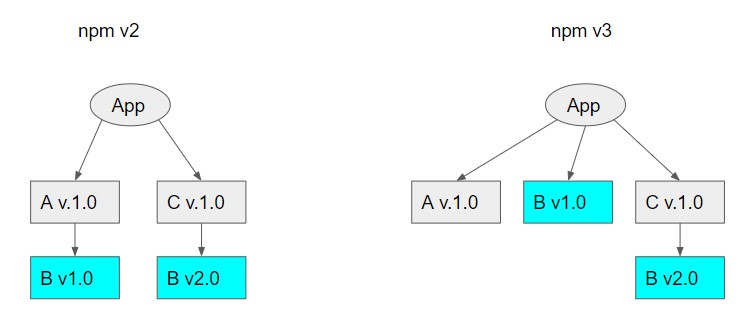
\includegraphics[width=.8\textwidth]{book/chapter-promisesandperils/pics/nestedv2.jpg}
	\caption{Difference between flat and nested dependencies}
	\label{fig:nest}
\end{figure}

\smallskip\noindent\textbf{Peril 5.}\textit{
Developers might declare a dependency to other parts of a software package ecosystem but not use it, e.g., because they failed to update its removal.
}\\

It is common for developers to declare dependencies on other parts of the software package ecosystem but not always use them. This can happen for various reasons, such as forgetting to remove the dependency after it is no longer needed. This can pose a challenge for researchers who are trying to extract dependencies from package managers, like those in configuration files, as there may be inconsistencies between the listed dependencies and what is actually being compiled and used by the code. This can lead to a biased understanding of the software package ecosystem and the relationships between software components.

To address this issue, there have been numerous efforts to track the actual library dependencies compiled and executed in software systems. These efforts aim to provide a more accurate understanding of the dependencies and the relationships between software components. For example, research has been conducted on the use of dynamic analysis to track compiled dependencies in real time and on the development of tools to automatically detect and track executed dependencies \cite{Zapata:ICSME2018, Ponta2018,Chinthanet:ASE2020}.

\subsection{Defining Boundaries and Completeness}

\smallskip\noindent\textbf{Promise 3.}\textit{
Researchers can use the boundaries of software package ecosystems to study communities of developers, e.g., developers contributing to and/or benefiting from the npm ecosystem.
}\\

Following Promise 2, the emergence of package managers has also led to studies that approximate software communities.
Using the libraries.io dataset, researchers were able to study projects that host libraries that use package managers.
Researchers have used this dataset to compare different library ecosystems \cite{kikas.2017,decan:emse:2019,CogoDown2019}.


\smallskip\noindent\textbf{Peril 6.}\textit{
Package managers do not always represent software package ecosystems, their communities, or their sub-communities, e.g., in cases where multiple package managers exist.
}\\

Package managers are a fundamental aspect of software package ecosystems, but do not always fully represent the complex relationships and interactions that occur within a community of developers and users, as shown in Table~\ref{tab:PM_features}. In some cases, multiple package managers exist for the same programming language, creating a complex landscape of software libraries and dependencies that are not always easily understood. For instance, Bower and Meteor manage npm libraries, which can lead to confusion and overlap in the management of dependencies.

Similarly, Java, Scala, Android, and other Java-based open source communities all use the Maven package manager, but each of these communities has its own unique set of libraries, dependencies, and development practises. Researchers should be aware of the limitations of package managers when studying software package ecosystems, and consider the broader context and relationships that exist within these communities. 

\smallskip\noindent\textbf{Peril 7.}\textit{
Lack of activity in parts of a software package ecosystem does not necessarily indicate project failure, e.g., when highly depended-upon libraries are feature-complete.
}\\

It is important to note that lack of activity in a part of a software package ecosystem does not always mean project failure \cite{coelho2017modern}. In some cases, highly relied-upon libraries that have reached feature-completeness may see little activity, but continue to be used by the software community. 

However, it is still important to consider the long-term sustainability of these libraries, especially given the rate at which technology and software development practises change. This has become a topic of interest in recent years, and researchers have explored best practises for sustaining open source projects and ensuring their continued success \cite{Ait2022,valiev2018ecosystem}. Understanding the factors that contribute to project sustainability is important to ensure the longevity and continued growth of software package ecosystems.

\smallskip\noindent\textbf{Peril 8.}\textit{
Sampling from a software package ecosystem is challenging since sub-setting might alter the dependency network, e.g., by breaking dependency chains.
}\\

Sampling from a package ecosystem is not straightforward, as the sample composition can be significantly affected due to missing dependency links between libraries. For instance, a subset of the ecosystem might alter the dependencies between libraries, leading to the breakdown of the dependency chains. This could lead to an incomplete picture of the software package ecosystem, leading to incorrect conclusions from a study. To minimise this risk, researchers should carefully consider the boundaries of their study and choose the appropriate sampling method based on the research questions and goals. For example, researchers could focus on popular, highly dependent, or risk-vulnerable aspects of the ecosystem as a starting point. 
For some ecosystems, the number of downloads, GitHub stars, and watchers are other aspects for the researcher to utilise.


\smallskip\noindent\textbf{Peril 9.}\textit{
Sampling from a software package ecosystem is challenging since the dependency network changes over time, e.g., when dependencies are added, removed, upgraded, or downgraded.
}\\

The dynamic nature of package ecosystems and the constant changes to their dependencies can impact the generalisability of the results. Therefore, it is important to also consider the time granularity of the analysis. For example, if the goal is to understand the evolution of dependencies over time, a finer time granularity may be necessary to capture the smaller changes and trends. However, if the goal is to understand the overall structure and relationships within the ecosystem, a coarser time granularity may be sufficient. Based on recent studies \cite{wattanakriengkrai2022giving,valiev2018ecosystem,Mirsaeedi:icse2020, Brindescu:emse2020, Nassif:icsme2017}, a three-month window seems appropriate for some studies.
Another level of granularity to consider is the size of the component. For instance, there are cases where a single package may contain more than one repository, especially for large library frameworks. 
The granularity also depends on the nature of the ecosystem itself. For instance, researchers should understand whether the ecosystem comprises library packages (e.g., PyPI), plugins (e.g., Eclipse), or is a library distribution (e.g., Android).



\subsection{Analysing and Visualising the Data}

\textbf{Peril 10.}\textit{
Analysing and visualising entire software package ecosystems is challenging due to their size, e.g., in terms of nodes and edges in the network.
}\\

The size of software package ecosystems implies large data sets, which can be overwhelming for tools and algorithms to analyse and display. Therefore, it may be necessary to make choices about the granularity of the data included in the analysis and visualisation. Another alternative is to focus on the most critical parts of the software package ecosystem, such as the high-level structure, highly dependent packages, or parts of the system that pose a risk to security and reliability. 
The key is to strike a balance between detail and simplicity, providing a meaningful representation of the ecosystem while being able to handle the complexity of its size.


\section{Application: When to Apply Which Peril}
\label{PPM:sec:application}

We include a disclaimer stating that not all perils are applicable to every mining situation. To demonstrate the practical application of our perils and their mitigation, we present two case studies that involve mining the software package ecosystem. Each case study has a distinct research objective and focusses on a specific dataset to be mined.

\subsection{Two Case Studies}
Table \ref{tab:cases} presents the two case studies we have selected for this analysis.
The \textit{first case} involves mining for contributions congruent to dependency updates \cite{wattanakriengkrai2022giving}. 
In this work, the authors mine GitHub repositories for Pull Requests and Issues that were submitted and merged congruent to dependency updates within the npm ecosystem. 
The \textit{second case} involves mining communication data for the Eclipse ecosystem \cite{Nugroho2021}. Although the second case does not mine for dependency relations (i.e., use relations),  we show that these perils still apply when mining for other relationships in an ecosystem.
Moreover, the second case studies the Eclipse ecosystem, which is a different dataset compared to the more popular GitHub dataset.

\subsection{Applying Perils and their Mitigation Strategies}
Table \ref{tab:perilsapp} provides a summary of the perils that can be applied to each of the case studies. We will now go into the details of mitigation strategies based on these perils. 
For better organisation and understanding, we have grouped the perils according to the four logical processes for mining.

\smallskip\noindent\textbf{Information to Mine}. 
The first set of mitigation strategies, which addresses perils 1-3, focusses on planning which information to mine. There are two primary strategies that researchers can employ:


\begin{enumerate}
    \item Researchers should use research tools and techniques to remove noise and other biases in the dataset, such as bot detection and the handling of multiple identities. This strategy was implemented in both case studies, as contributions and discussions often have the potential to involve bots or developers with multiple identities.
\item Depending on the research goals, researchers should recognise that not all contributions are equal and filter the dataset accordingly.
\end{enumerate}

We applied these two strategies to both cases. In the first case, the goal was to capture all congruent contributions, so we filtered out contributions made to libraries without dependencies. Since all npm packages are listed in the registry, Peril 3 (private activities) did not apply.
In the second case, we addressed Peril 1 by conducting a qualitative analysis to ensure that the member identities were not duplicated, as Eclipse developers were known to change identities. To mitigate Peril 2, we removed bot responses. For the second case, since all forum data is made public, Peril 3 did not apply.


\begin{table}
\centering
\caption{Description of the research objectives and datasets for the case studies}
 \label{tab:cases}
\begin{tabular}{lp{5cm}r} 
\toprule
\textbf{Case Study} & \textbf{Research Objective}                                                          & \textbf{Datasets}           \\
\midrule
Wattanakriengkrai \etal \cite{wattanakriengkrai2022giving}             & Explore code contributions between library and client (i.e, use-relations)  & libraries.io\\
& &  GitHub API \\
Nugroho \etal \cite{Nugroho2021}                & Explore discussion contributions between contributors (i.e., contributions) & Eclipse API                \\
\bottomrule
\end{tabular}
\end{table}

\begin{table}
\centering
\caption{Application of each peril to the case studies}
 \label{tab:perilsapp}
\begin{tabular}{rp{8cm}ccc} 
\toprule                   
& \textbf{Perils}       & case 1      & case 2                 \\
                                                                               & & npm  & Eclipse   \\
\midrule
\textbf{P1} &Developers might use different identifiers when contributing to different parts of a software package ecosystem, e.g., when contributing to different libraries.                             &    \CheckedBox         &          \CheckedBox           \\ 
%\hline
\textbf{P2} & Developers' contributions to software package ecosystems might be interspersed with bot contributions, e.g., automated dependency updates.                                                      &      \CheckedBox               &      \CheckedBox               \\ 
%\hline
\textbf{P3} & Not all developer activities in software package ecosystems are accessible to the public, e.g., library use in proprietary settings.                                                         &         -           &      \CheckedBox               \\ 
%\hline
\textbf{P4} & Different software package ecosystems define the concept of \`{}\`{}dependency'' differently, e.g., by allowing or not allowing different versions of a library on the same dependency tree. &         \CheckedBox       &     -                            \\ 
%\hline
\textbf{P5} & Developers might declare a dependency to other parts of a software package ecosystem but not use it, e.g., because they failed to update its removal.                                        &     -           &  -    \\
%\hline
\textbf{P6} &Package managers do not always represent software package ecosystems, their communities, or their sub-communities, e.g., in cases where multiple package managers exist.                     &     -                   &  -                  \\
%\hline
\textbf{P7} & Lack of activity in parts of a software package ecosystem does not necessarily indicate project failure, e.g., when highly depended-upon libraries are feature-complete.                     &       \CheckedBox         &  -                           \\
%\hline
\textbf{P8} &Sampling from a software package ecosystem is challenging since sub-setting might alter the dependency network, e.g., by breaking dependency chains.                                         &        \CheckedBox        &     \CheckedBox                                \\
%\hline
\textbf{P9} &Sampling from a software package ecosystem is challenging since the dependency network changes over time, e.g., when dependencies are added, removed, upgraded, or downgraded.               &       \CheckedBox         &     -                          \\
%\hline
\textbf{P10} &Analysing and visualising entire software package ecosystems is challenging due to their size, e.g., in terms of nodes and edges in the network.                                  &        \CheckedBox      &      \CheckedBox               \\
\bottomrule
\end{tabular}
\end{table}

\smallskip\noindent\textbf{Defining Dependencies}. 
The second set of perils (Perils 4-5) is related to dependency relationships between software units, and only the first case study is applicable. To address these perils, researchers should adopt the following strategy:

\begin{enumerate}
    \item Researchers should not rely solely on listed dependencies in configuration files (e.g., pom.xml, package.json, etc.) as a measure of dependency between two components. Instead, code-centric approaches should be used to validate which libraries are actually depended upon.
\end{enumerate}

For example, in the first case, in addition to mining the configuration information, the authors also analysed the similarity of the source code contributions to address Peril 4. Regarding Peril 5, since the study's objective was to investigate changes to the configuration files, the risk of the update not being executed was deemed less important.
It is important to note that the second case study did not include dependency analysis and, therefore, these perils did not apply.

\begin{figure*}[]
    \centering
    \begin{subfigure}{0.9\linewidth}
         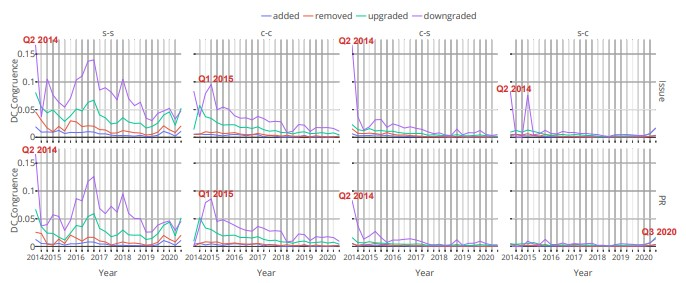
\includegraphics[width=1.1\textwidth]{book/chapter-promisesandperils/pics/congruentViz.jpg}
         \caption{Visualization of a Time analysis for 107,242 libraries.}
     \end{subfigure}
     \begin{subfigure}{0.9\linewidth}
         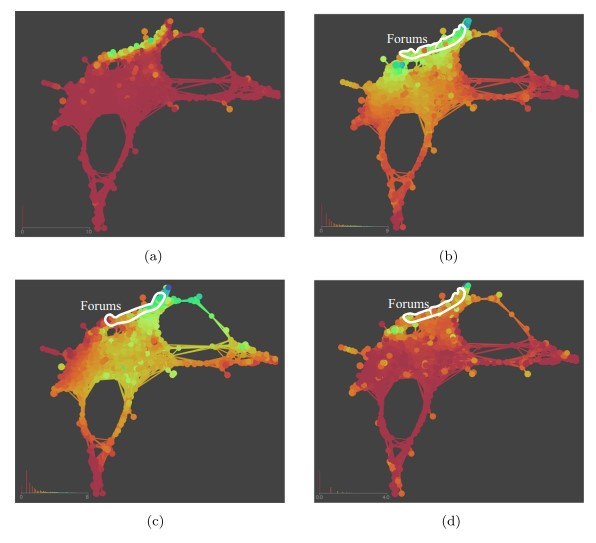
\includegraphics[width=1\textwidth]{book/chapter-promisesandperils/pics/eclipseViz.jpg}
         \caption{A Visual Topology map for 832,058 threads}
     \end{subfigure}
    \caption{Visualisation examples for the two case studies}
    \label{fig:visCase}
\end{figure*}

\smallskip\noindent\textbf{Defining Boundaries}.
The third set of perils (Perils 6-9) is related to the definition of boundaries and completeness and is relevant for both case studies. To mitigate these perils, we recommend the following strategies:

\begin{enumerate}
    \item Researchers should recognise that a dormant project does not necessarily mean that it is inactive. Instead, studies can use alternative heuristics, such as the number of dependents and dependencies, as better indicators of a project's importance in the ecosystem.
    \item Researchers should not rely solely on the programming language to define sub-communities. Using a common package manager for the programming language is a more effective rule of thumb for distinguishing boundaries.
    \item Researchers should avoid random sampling. Instead, sampling should be tailored to the research goals by considering factors such as an appropriate time window or focussing on specific attributes of components (e.g., most dependents, most popular, most contributors).
\end{enumerate}


Peril 6 did not apply to any of the case studies. 
Particularly for the first case, since the goal was to explore the npm package ecosystem, we assumed that the boundaries were clearly defined by the npm registry. 
Similarly, the second case study used the generic Eclipse platform as the boundary. 
Peril 7 was applied to the npm study, while Peril 8 was applied to both case studies. 
As a result, the two cases conducted a qualitative analysis of the dataset to gain deeper insights.
In the first case study, a three-month time window was created to capture dependencies. 
For the second case study, forum contributors were sampled into three groups (i.e., junior, member, or senior) according to the sliding window of their contributions. 

\smallskip\noindent\textbf{Visualisation}.
The final peril (Peril 10) relates to visualisation, which can be challenging due to the vast size and complexity of software ecosystems. As it is not feasible to visualise every aspect of an ecosystem simultaneously, a focused approach is necessary. A mitigation strategy is to select specific attributes of the ecosystem (e.g., the most dependent, most popular, and most contributions) that align with the research needs and objectives. 

Figure \ref{fig:visCase} shows two cases where visualizations are employed to gain insights, especially for large datasets.
In the first figure (a), we visualize the distributions of the data set and applied the appropriate statistical tests, along with the effect size, to test our hypotheses and answer research questions. 
In the second example (b), although not directly related to package ecosystems, the authors utilized a topological visualization \cite{Lum2013ExtractingIF} to gain insights on the over 800,000 forum threads of discussions. 



\section{Chapter Summary}
In this chapter, we explore the various aspects of mining information from the software package ecosystem, presenting three promises and ten perils that researchers should be aware of when undertaking such tasks. The chapter is structured around four key processes for mining: 1) Planning what Information to Mine, 2) Defining Components and their Dependencies, 3) Defining Boundaries and Completeness, and 4) Analysing and Visualising the Data. To help new and experienced researchers navigate these challenges, we introduced the SUG model, which can serve as a valuable tool to minimise threats to validity. Although some perils may be more relevant to specific research objectives, our aim is to equip researchers with the knowledge and resources needed to confidently gather and integrate software package ecosystem data into their work.
%Supporting Collateral Evolution in Software Development Ecosystems
% %Semantic labeling three-letter-code: COL (e.g. \chapter{COL})


% %%%%%%%%%%%%%%%%%%%%%part.tex%%%%%%%%%%%%%%%%%%%%%%%%%%%%%%%%%%
% 
% sample part title
%
% Use this file as a template for your own input.
%
%%%%%%%%%%%%%%%%%%%%%%%% Springer %%%%%%%%%%%%%%%%%%%%%%%%%%

\begin{partbacktext}
\part{PROCESS-CENTERED SOFTWARE ECOSYSTEMS}
\label{part:process}


\end{partbacktext} %PROCESS-CENTERED SOFTWARE ECOSYSTEMS
% 
\title{Promises and Perils of Mining \\ Software Package Ecosystem Data}
\author{Raula Gaikovina Kula \and Katsuro Inoue \and Christoph Treude}
\institute{Raula Gaikovina Kula \at Nara Institute of Science and Technology, Japan, \email{raula-k@naist.jp}
\and Katsuro Inoue \at Nanzan University, Japan \email{ inoue599@nanzan-u.ac.jp}
\and  Christoph Treude \at The University of Melbourne, Australia \email{christoph.treude@unimelb.edu.au}}

\maketitle
\label{PPM:ch}
\abstract*{The use of third-party packages is becoming increasingly popular and has led to the emergence of large software package ecosystems with a maze of inter-dependencies. Since the reliance on these ecosystems enables developers to reduce development effort and increase productivity, it has attracted the interest of researchers: understanding the infrastructure and dynamics of package ecosystems has given rise to approaches for better code reuse, automated updates, and the avoidance of vulnerabilities, to name a few examples. But the reality of these ecosystems also poses challenges to software engineering researchers, such as: How do we obtain the complete network of dependencies along with the corresponding versioning information? What are the boundaries of these package ecosystem? How do we consistently detect dependencies that are declared but not used? How do we consistently identify developers within a package ecosystem? How much of the ecosystem do we need to understand to analyse a single component? How well do our approaches generalise across different programming languages and package ecosystems? In this chapter, we review promises and perils of mining the rich data related to software package ecosystems available to software engineering researchers.}

\abstract{The use of third-party packages is becoming increasingly popular and has led to the emergence of large software package ecosystems with a maze of inter-dependencies. Since the reliance on these ecosystems enables developers to reduce development effort and increase productivity, it has attracted the interest of researchers: understanding the infrastructure and dynamics of package ecosystems has given rise to approaches for better code reuse, automated updates, and the avoidance of vulnerabilities, to name a few examples. But the reality of these ecosystems also poses challenges to software engineering researchers, such as: How do we obtain the complete network of dependencies along with the corresponding versioning information? What are the boundaries of these package ecosystems? How do we consistently detect dependencies that are declared but not used? How do we consistently identify developers within a package ecosystem? How much of the ecosystem do we need to understand to analyse a single component? How well do our approaches generalise across different programming languages and package ecosystems? In this chapter, we review promises and perils of mining the rich data related to software package ecosystems available to software engineering researchers.}

%%%%%%%%%%%%%%%%%%%%%%%%%%%%%%%%%%%%%%%%%%%%%%%%%%%%%%%%%%%%%%%%%%

\section{Introduction}
\label{PPM:sec:definition}

Third-party libraries are a great way for developers to incorporate code without having to write their own for every functionality required. By using these libraries, developers can save time and energy while still getting the functions they need.
Using third-party libraries is becoming increasingly popular and has led to the emergence of large software package ecosystems such as npm. While these ecosystems offer many benefits, they also come with risks, such as software vulnerability attacks \cite{Chinthanet:ASE2020}.

Large software package ecosystems are a treasure trove for researchers who can investigate a wide range of questions. For example, by studying activity in large ecosystems, researchers can identify which libraries are the most popular and learn what characteristics make them successful \cite{kikas.2017,decan:emse:2019}.
Additionally, research on large ecosystems can help developers understand how to protect their code from malicious actors who may attempt to exploit vulnerabilities or insert malware into popular libraries.
Studying large software package ecosystems can help us better understand the dynamics of open source development in general. Open source development is a complex process that involves many different stakeholders working together (or sometimes competing) to create valuable code that anyone can use or improve upon. By understanding how these interactions play out in different types of ecosystem structures -- including those with many small projects versus few very large ones -- we can develop insights that might be applicable more broadly across other types of collaborative systems.

In this chapter, we identify and discuss promises and perils during the mining process, ranging from planning what information to mine from the ecosystem to analysing and visualising the mined data. 
Therefore, the chapter is broken down into these logical processes of mining ecosystem data: 1) Planning what Information to Mine, 2) Defining Components and their Dependencies, 3) Defining Boundaries and Completeness, and 4) Analysing and Visualising the Data.

This chapter is intended for researchers and practitioners who are interested in exploring and exploiting software package ecosystem information from a diverse range of sources that are publicly available. 
We also highlight the pitfalls to consider during the mining process, particularly when these pitfalls could lead to a misinterpretation of the analysis and results. 
The chapter is written in a manner that encourages newcomers who have little or no experience or who are interested in utilising ecosystem data across different disciplines outside of software engineering.
Our goal is to get new researchers quickly accustomed to gathering ecosystem information for their research.


\section{A Component-based Software Ecosystem}

Defined as a component-based software ecosystem, we suggest using the term `software package ecosystem' as a suitable term for the symbiotic relationships among third-party library components (as software projects or repositories), as these libraries and their dependent clients coexist on the same technological platform, therefore sharing the same environment and other internal and external factors (e.g., security threats, sharing contributions, etc.).
Please refer to the Introduction chapter for an in-depth definition of the different types of software ecosystems.
We present our interpretation of the software package ecosystem in Kula et al.~\cite{KulaSANER18}, where we formally define a package ecosystem using a Software Universe Graph (SUG).
This is modelled as a structured abstraction of the evolution of software systems and their library dependencies over time.

%%%%%%%%%%%%%%%%%%%%%%%%%%%%%%%%%%%%%%%%%%
\begin{figure*}
	\centering
	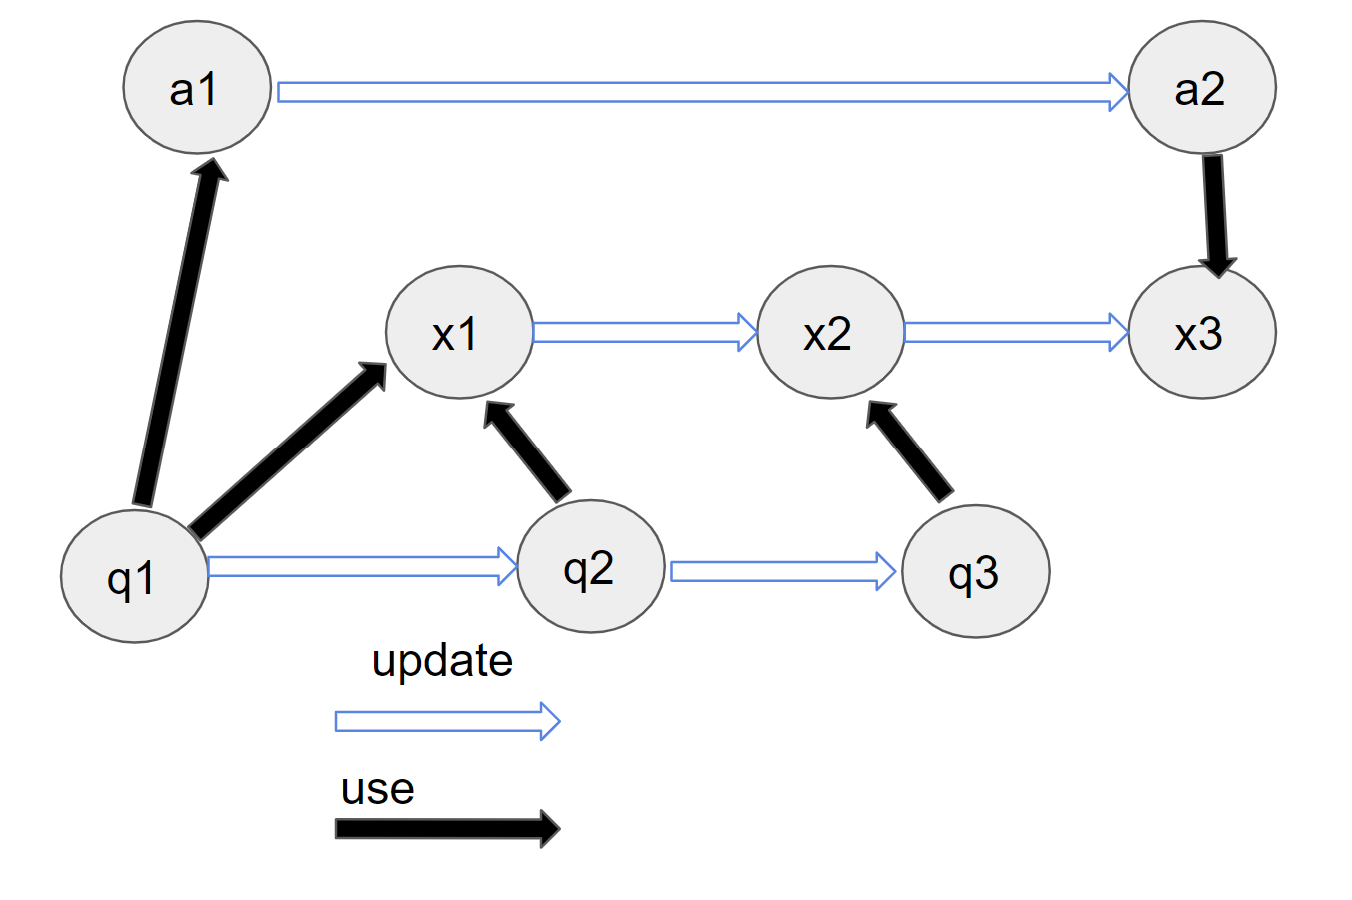
\includegraphics[width=.7\textwidth]{book/chapter-promisesandperils/pics/UniversalExample.jpg}
	\caption{Conceptual example of the Software Universe Graph, depicting the use and update relationships between different software units.}
	\label{fig:SUG}
\end{figure*}
%%%%%%%%%%%%%%%%%%%%%%%%%%%%%%%%%%%%%%%%%%%%%


\paragraph{\textbf{Component-based Representation as a Software Universe Graph}}
\label{PPM:sec:SUG}

First introduced by Kula et al.~\cite{KulaSANER18}, the \textit{Software Universe Graph} (SUG) is a structural abstraction of the software ecosystem of third-party libraries.
Figure \ref{fig:SUG} provides an illustration of the different relationships within the graph.
Let $G= (N,E)$ represent a graph $G$. $N$ is a set of nodes, each node representing a software unit. 
We define a software unit as a version instance of any software program. 

The authors then present the \textit{use} and \textit{update} relationships that exist in the ecosystem.
Hence, the edges $E$ are composed of $E_{use}$ and $E_{update}$. $E_{use}$ is a set of \textit{use-relations} and $E_{update}$ is a set of \textit{update-relations}.

\begin{definition}
An edge $u \rightarrow v \in E_{use}$ means that $u$ uses $v$. The defined functions of $E_{use}$ are:

\begin{equation}
\small
\small \use(u)\equiv \{v|u \rightarrow v\}
\normalsize
\end{equation}
\begin{equation}
\small
\small \useBy(u)\equiv \{v|v \rightarrow u\}
\normalsize
\end{equation}
\end{definition}

Use-relations can be extracted from either the source code or configuration files. 
As shown in Figure \ref{fig:SUG}, node $a1$ uses node $x1$. 
In addition, node $x1$ is used by nodes $a1$, $q1$, and $q2$. Parallel edges for node pairs are not allowed.

\begin{definition}
We represent an update relation from node $a$ to $b$ using $ a \Rightarrow b $, which means that the newer update $b$ was released from node $a$ and is defined as:
\begin{equation}
\small a \Rightarrow b \in E_{update}
\end{equation}
\end{definition}

Update relations refer to when a successive release of a software unit is made available. Figure \ref{fig:SUG} shows that node $q1$ is first updated to node $q2$. Later, node $q2$ is updated to the latest node $q3$. Hence, $q1 \Rightarrow q2 \Rightarrow q3$.
Note that an update should not be confused with forking. 
We distinguish a fork as a separate software unit. 
Each node in the SUG should be denoted by three attributes: \texttt{<name,release,time>}.  
For a node $u$, we define:

\begin{itemize}
	\item \textbf{u.name} Name is the string representation identifier of a software unit.
	We introduce the name axiom: For nodes $u$ and $v$, if $u \Rightarrow v$, then $u.name = v.name$ holds.
	
	\item \textbf{u.release}. Release refers to the specific assigned change reference for a software unit. For nodes $u$ and $v$, if $u \Rightarrow v$
	then $v$ is the immediate successor of $u$. Note that the versioning pattern may vary from project to project. 
	\item \textbf{u.time}. Time refers to the time stamp at which node $u$ was released. For nodes $u$ and $v$ of $u \Rightarrow v$, $u.time < v.time$.
\end{itemize}

\begin{figure}
	\centering
	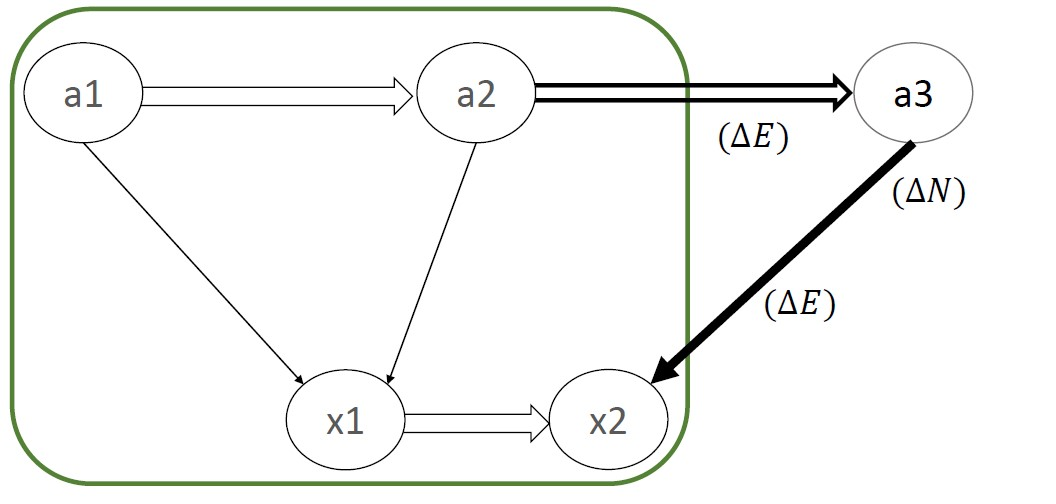
\includegraphics[width=.8\textwidth]{book/chapter-promisesandperils/pics/TemporalSUG.jpg}
	\caption{Temporal property of the SUG}
	\label{fig:SUGTemp}
\end{figure}

\begin{definition}
    
	The SUG has temporal properties.
This describes the simultaneity or ordering in reference to time. Let SUG $G = (N, E) $ be at time $t$. At time $t^{\prime} > t$, we observe an extension of $G$, such that:

\begin{equation}
\small G^{\prime} = (N \cup \Delta N, E \cup \Delta E)
\end{equation}
where $\Delta E \cap (N \times N) = \emptyset$
\end{definition}

Figure \ref{fig:SUGTemp} illustrates the temporal properties of the SUG. 
Here, it is observed that $G'$ is composed of $G$ augmented with newly added node $a3$ and its corresponding $a3 \rightarrow x2$ and $a2 \Rightarrow a3$ relations.
A SUG grows monotonically over time with only additions.
Here, we consider that modification or deletion changes on the SUG do not occur. 

\begin{definition}
    A timed SUG specifies the state of the SUG at any point in time.
So for an SUG $G=(N,E)$, we represent a timed SUG $G_{t}$ at time $t$ as a sub-graph of $G$. Formally,
\begin{equation}
\small G_t\equiv(N_{t}, E_{t})
\end{equation}
where $N_{t} = \{u|u \in N, u.time \leq t \}$ and $E_t = \{ e | e \in E \wedge e \in  N_t \}$
\end{definition}
	


\section{Data Sources}
Researchers can use various datasets to model the ecosystem using the SUG model of usage and update relationships.
The most obvious data source that has revolutionised data mining in the software engineering domain is the GitHub platform. 
Established in 2008, and then purchased by Microsoft in 2020, GitHub is home to various popular Open Source Software. 
GitHub is built on the git version control system and is useful for storing all changes made to a repository. 
In the case of the SUG, a GitHub repository can represent one software unit, whose depend relations can be extracted via a configuration file (such as the package.json file for JavaScript projects).
The repository should also contain the release information that holds the update relations.
Due to its large size, researchers and the GitHub team have made available datasets for researchers to mine, for example through the GitHub API/Graph QL.\footnote{\url{https://docs.github.com/en/graphql}} This is the backend Application Programming Interface (API) that can be used to query large amounts of data on GitHub. Most researchers use the API to download and mine information from the GitHub platform. 
It is important to note that while GitHub introduced a new feature of Dependency Graphs to map the depend relationship,\footnote{\url{https://docs.github.com/en/code-security/supply-chain-security/understanding-your-software-supply-chain/about-the-dependency-graph}} most older projects do not have this feature.
In this case, the researcher would need to manually extract and query the configuration files for dependency information. 

We refer to the first chapter for additional information on data sources for mining software ecosystems. 

\section{Promises and Perils}
\label{PPM:sec:promisesperils}

Using the SUG model of depend and use relations and the available datasets, we can now present our promises and perils of mining ecosystem information.

\subsection{Planning What Information to Mine}

\textbf{Promise 1.}\textit{
Researchers can access and link heterogeneous data related to software package ecosystems, e.g., package registries and bug trackers.}\\

When planning what information to mine from the ecosystem, researchers do not need to limit themselves to the usage and update relationship information.
Platforms that host software repositories include other software management systems such as bug trackers.
For example, GitHub allows researchers to manage GitHub Pull Requests, Issues, and Discussions not only for one project, but for multiple projects.
GitHub provides three management systems that are related to a software repository:

\begin{itemize}
    \item \textit{GitHub Discussions}\footnote{\url{https://docs.github.com/en/discussions}} - The GitHub Discussions forum is a collaborative communication forum for the community around an open source or internal project. Community members can ask and answer questions, share updates, have open-ended conversations, and follow along on decisions affecting the community's way of working.
    \item \textit{GitHub Pull Requests}\footnote{\url{https://docs.github.com/en/pull-requests}} - Pull Requests allow other developers from an ecosystem to make a contribution to a software repository. Pull requests also allow maintainers to discuss and review potential changes with collaborators and add follow-up commits before changes are merged into the software.
    \item \textit{GitHub Issues}\footnote{\url{https://docs.github.com/en/issues}} - Issues are used to track ideas, feedback, tasks, or bugs for work on GitHub.
\end{itemize}

These three systems are examples of how developers contribute to both their own and other projects. 
Hence, to incorporate this information, we can extend the SUG model, creating a model that includes a contribution relationship \cite{wattanakriengkrai2022giving}.

% Note that other platforms may also have management systems, like GitLab, BitBucket and Eclipse.

\begin{definition}
	A Dependency-Contribution graph incorporates contributions by developers whose libraries are involved in dependency relationships. 
\end{definition}

In this work \cite{wattanakriengkrai2022giving}, the authors explore the congruence between dependency updates and developer contributions, based on the original concept of social-technical congruence \cite{stcCataldo2008} where developers contribution patterns are congruent with their coordination needs. Hence, the goal is to identify contributions that are congruent to dependency updates.
As shown in Figure \ref{fig:lib} the authors extend from the typical SUG graph model where $lib_i$ depends (use) on  $lib_k$ and  $lib_j$, while  $lib_j$ also depends on $lib_k$, to the example shown in Figure \ref{fig:dc-graph}.
Different to the SUG, the graph captures developers and their contributions (i.e., the square as $dev_x$ and $dev_y$ represent two different developers making a contribution).
Here contributions are defined as $c$ (Pull Request or Issue) that were submitted to both a library and the client that depends on that library.
Hence, the graph can show contributions that are congruent to dependency changes for a software unit. 

\begin{figure}[t]
     \centering
     \begin{tikzpicture}[
         roundnode/.style={circle, fill=black, minimum size=5mm},
        squarenode/.style={fill=black, text=red, minimum size=5mm},
     ]
    \begin{scope}
         \node[roundnode, label=above:$lib_i$] (s2_proji) at (3, 2.5) {};
        \node[roundnode, label=below:$lib_j$] (s2_projj) at (4,0) {};
         \node[roundnode, label=below:$lib_k$] (s2_projk) at (2,0) {};
     \end{scope}

     \begin{scope} [every edge/.style={draw=gray, very thick}]
         \path [->] (s2_proji) edge (s2_projj);
         \path [->] (s2_proji) edge (s2_projk);
         \path [->] (s2_projj) edge (s2_projk);
     \end{scope}
     \end{tikzpicture}
    
     \caption{Example dependency graph for a given time period}
     \label{fig:lib}
     \vspace{2ex}
 \end{figure}
\begin{figure}[t]
    \centering

    \begin{tikzpicture}[
        roundnode/.style={circle, fill=black, minimum size=5mm},
        squarenode/.style={fill=black, text=red, minimum size=5mm},
    ]
    \begin{scope}
        
        \node[roundnode, label=right:$lib_i$] (s2_proji) at (4, 1.5) {};
        \node[roundnode, label=below:$lib_j$] (s2_projj) at (5,0) {};
        \node[roundnode, label=below:$lib_k$] (s2_projk) at (3,0) {};
        
        \node[squarenode, label=below:$dev_x$] (s3_devx) at (2, 3.5) {};
        
        \node[squarenode, label=below:$dev_y$] (s3_devy) at (6, 3.5) {};
        
    \end{scope}

    \begin{scope} [every edge/.style={draw=gray, very thick}]
        \path [->] (s2_proji)  edge  (s2_projj);
        \path [->] (s2_proji) edge (s2_projk);
        \path [->] (s2_projj) edge (s2_projk);
        
    \end{scope}
    \begin{scope} [every edge/.style={draw=gray, thick, double distance=2pt}]
        \path [->] (6, 2.8) edge node[left = 2mm] {$contribute$} (s2_proji);
        \path [->] (6, 2.8) edge[bend left=15] node[right = 1mm] {$contribute$} (s2_projj);
        \path [->] (2, 2.8) edge node[right = 2mm] {$$} (s2_proji);
        \path [->] (2, 2.8) edge[bend right=15] node[left = 1mm] {$contribute$} (s2_projk);
    \end{scope}
    \end{tikzpicture}
\end{figure}
\begin{figure}[t]
    \centering
    \begin{tikzpicture}[
        roundnode/.style={circle, fill=black, minimum size=5mm},
        squarenode/.style={fill=black, text=red, minimum size=5mm},
    ]
    \end{tikzpicture}
\caption{Example Dependency-Contribution graph showing relationships between contributions and dependencies}
 \label{fig:dc-graph}
\end{figure}

This is just one example of the type of research that is enabled by access to heterogeneous data related to software package ecosystems.

\smallskip\noindent\textbf{Peril 1.}\textit{
 Developers might use different identifiers when contributing to different parts of a software package ecosystem, e.g., when contributing to different libraries.}\\
 
When modelling using such graphs, there is a threat that contributors may use multiple identifiers (i.e., $c_x$ and $c_y$ are the same contributor).
This is a well-known research problem, and there has been work to merge these accounts, such as \cite{wiese2016mailing}.
GitHub has introduced mechanisms such as two-factor authentication\footnote{\url{https://docs.github.com/en/authentication/securing-your-account-with-two-factor-authentication-2fa/configuring-two-factor-authentication}} to counteract the issue of multiple identifiers.
This is since developers might be less likely to switch accounts if it requires cumbersome authentication.


\smallskip\noindent\textbf{Peril 2.}\textit{
Developers' contributions to software package ecosystems might be interspersed with bot contributions, e.g., automated dependency updates.}\\

The rise of automation and artificial intelligence has led to much work on the integration of automated scheduling (i.e., bots) into software development workflows \cite{Storey2016, Farooq2016, Wessel2018, Erlenhov2019, bot_modify_wf} to name a few. These bots are designed to perform specific tasks within a software package ecosystem. For example, a bot may be programmed to automatically update dependencies, test code changes, or deploy software to production. As an example, the Google APIs repo-automation-bots project lists bots for automated labelling of issues and pull requests, automated approval of pull requests, and triggering releases.\footnote{\url{https://github.com/googleapis/repo-automation-bots}}
Bots perform common maintenance tasks in many software projects and are now commonplace \cite{Beschastnikh2017, Urli2018,BIMAN,bot_or_not}.
Especially with bots such as dependabot (automated pull requests to update configurations to reduce the risk of vulnerability threats),\footnote{\url{https://github.com/dependabot}} more and more automation has caused a lot of noise in the contributions between projects.
There are also bots for communication and documentation \cite{Urli2018, Lin2016, Lebeuf2017a}.

To be able to draw accurate conclusions about what humans are doing in software package ecosystems, researchers should consider distinguishing between bot and human contributions.
It is also important to differentiate this from other contributions \cite{maeprasart2022understanding}.
The research community has responded well, with a wide range of techniques and tools to mitigate this peril \cite{Bodegha2021, golzadeh2022accuracy}.

\smallskip\noindent\textbf{Peril 3.}\textit{
Not all developer activities in software package ecosystems are accessible to the public, e.g., library use in proprietary settings.
}\\

Not all developer activities in software package ecosystems are accessible to the public, e.g., when the boundary between open source and industry is blurred \cite{stol2014inner}, which presents a challenge for researchers who aim to study the development process. This is particularly true in proprietary settings where software development is performed behind closed doors or is open source for a limited time period, thus resulting in the artefacts not permanently being publicly available.
This can make it difficult to understand the broader ecosystem in which a software project is developed.
Proprietary settings may lead to non-standardisation in software development practises. Different software projects may use different management systems and tools, making it difficult to accurately compare and analyse software development activities across various projects. For example, some projects may use communication, documentation, and other management tools not captured on the same platform \cite{montgomery2022alternative}. For example, some projects might use Bugzilla instead of issues and pull requests for their bug and code review systems, while others may use Discord, Slack channels, or email threads for their communication needs.

This lack of standardisation in software development practises presents a challenge for researchers who study the software package ecosystem and understand the development process. To address this issue, researchers should strive to collect data from a diverse set of projects to gain a comprehensive understanding of the software package ecosystem. In addition, researchers may need to adjust their methodologies or data collection techniques to accommodate the different tools and practises used by different software projects.

\subsection{Defining Components and their Dependencies}

\smallskip\noindent\textbf{Promise 2.}\textit{
Researchers can access a software package ecosystem's dependency network through package managers and registries, e.g., npm lists the dependencies and dependents for over a million libraries.}\\


With the rise of curated datasets like libraries.io, researchers can now recover and model dependency relations between software units using pre-extracted datasets.
Table \ref{tab:PM_features} shows examples of popular package managers mined from the libraries.io dataset in 2020. 

\begin{table*}[]
\caption{Summary of 13 package managers from libraries.io as ranked by TIOBE in 2020}
 \label{tab:PM_features}
 \centering
\begin{tabular}{@{}llrlll@{}}
\toprule
\begin{tabular}[c]{@{}l@{}}Package \\ Ecosystem\end{tabular} & \begin{tabular}[c]{@{}l@{}}Programming \\ Language\end{tabular} &  \begin{tabular}[c]{@{}l@{}}Tiobe \\ Rank\end{tabular} & Environment & \begin{tabular}[c]{@{}l@{}}Dependency \\ Tree\end{tabular} & \begin{tabular}[c]{@{}l@{}}Package   \\Archive link\end{tabular}\\ \midrule
PyPI & Python & 2 & Python & Flat & pypi.org  \\
Maven & Java & 3 & JVM & Flat & Maven.org  \\
Bower & JavaScript & 7 & Node.js & Flat & bower.io  \\
Meteor & JavaScript & 7 & Node.js & Nested & atmospherejs.com \\
npm & JavaScript & 7 & Node.js & Nested (v2) & npmjs.com  \\
Packagist & PHP & 8 & PHP & Flat & packagist.org \\
Puppet & Ruby & 13 & Ruby MRI & Flat & forge.puppet.com  \\
RubyGems & Ruby & 13 & Ruby MRI & Flat & rubygems.org  \\
CRAN & R & 14 & RStudio & Flat & cran.r-project.org  \\
CPAN & Perl & 15 & Perl & Flat & metacpan.org  \\
GO & Golang & 20 & Go & Flat & pkg.go.dev  \\
NuGet & C\#, VB & 5, 6 & .NET & Flat & nuget.org \\
Anaconda & Python, R, C\# & 2, 14, 5 & Anaconda & Flat & anaconda.org  \\ \bottomrule
\end{tabular}
\end{table*}

\smallskip\noindent\textbf{Peril 4.}\textit{
Different software package ecosystems define the concept of ``dependency'' differently, e.g., by allowing or not allowing different versions of a library on the same dependency tree.
}\\

Different software package ecosystems have varying definitions of what constitutes a dependency. For example, some ecosystems may allow multiple versions of a library to exist on the same dependency tree, while others may restrict developers to a single version of a library \cite{Islam}. These restrictions are often based on the programming language being used, as different languages have different approaches to managing dependencies. It is important to consider the restrictions on dependency relationships when studying software package ecosystems, as they can have a major impact on the development process. For example, the ability to use multiple versions of a library on the same dependency tree can greatly simplify the process of updating dependencies and can make it easier to resolve conflicts between libraries.

One way to visualise the impact of these restrictions is to compare the difference between a nested dependency tree and a directed dependency tree, as shown in Figure \ref{fig:nest}.\footnote{Taken from \url{https://npm.github.io/how-npm-works-docs/npm3/how-npm3-works.html}} This distinction is important because it highlights the different ways that a software unit can depend on different versions of the same library.
In this example, npm v3 creates the dependency tree based on the installation order, therefore flattening unnecessary nested dependencies (i.e., B v1.0 in cyan). This reduces the complexity of a nested tree by resolving some of the transitive dependencies (nested dependencies).

\begin{figure}
	\centering
	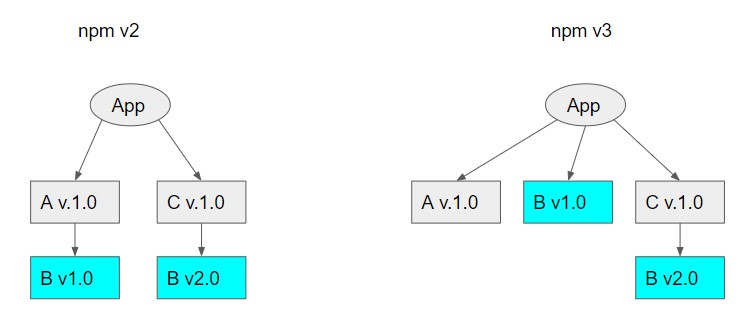
\includegraphics[width=.8\textwidth]{book/chapter-promisesandperils/pics/nestedv2.jpg}
	\caption{Difference between flat and nested dependencies}
	\label{fig:nest}
\end{figure}

\smallskip\noindent\textbf{Peril 5.}\textit{
Developers might declare a dependency to other parts of a software package ecosystem but not use it, e.g., because they failed to update its removal.
}\\

It is common for developers to declare dependencies on other parts of the software package ecosystem but not always use them. This can happen for various reasons, such as forgetting to remove the dependency after it is no longer needed. This can pose a challenge for researchers who are trying to extract dependencies from package managers, like those in configuration files, as there may be inconsistencies between the listed dependencies and what is actually being compiled and used by the code. This can lead to a biased understanding of the software package ecosystem and the relationships between software components.

To address this issue, there have been numerous efforts to track the actual library dependencies compiled and executed in software systems. These efforts aim to provide a more accurate understanding of the dependencies and the relationships between software components. For example, research has been conducted on the use of dynamic analysis to track compiled dependencies in real time and on the development of tools to automatically detect and track executed dependencies \cite{Zapata:ICSME2018, Ponta2018,Chinthanet:ASE2020}.

\subsection{Defining Boundaries and Completeness}

\smallskip\noindent\textbf{Promise 3.}\textit{
Researchers can use the boundaries of software package ecosystems to study communities of developers, e.g., developers contributing to and/or benefiting from the npm ecosystem.
}\\

Following Promise 2, the emergence of package managers has also led to studies that approximate software communities.
Using the libraries.io dataset, researchers were able to study projects that host libraries that use package managers.
Researchers have used this dataset to compare different library ecosystems \cite{kikas.2017,decan:emse:2019,CogoDown2019}.


\smallskip\noindent\textbf{Peril 6.}\textit{
Package managers do not always represent software package ecosystems, their communities, or their sub-communities, e.g., in cases where multiple package managers exist.
}\\

Package managers are a fundamental aspect of software package ecosystems, but do not always fully represent the complex relationships and interactions that occur within a community of developers and users, as shown in Table~\ref{tab:PM_features}. In some cases, multiple package managers exist for the same programming language, creating a complex landscape of software libraries and dependencies that are not always easily understood. For instance, Bower and Meteor manage npm libraries, which can lead to confusion and overlap in the management of dependencies.

Similarly, Java, Scala, Android, and other Java-based open source communities all use the Maven package manager, but each of these communities has its own unique set of libraries, dependencies, and development practises. Researchers should be aware of the limitations of package managers when studying software package ecosystems, and consider the broader context and relationships that exist within these communities. 

\smallskip\noindent\textbf{Peril 7.}\textit{
Lack of activity in parts of a software package ecosystem does not necessarily indicate project failure, e.g., when highly depended-upon libraries are feature-complete.
}\\

It is important to note that lack of activity in a part of a software package ecosystem does not always mean project failure \cite{coelho2017modern}. In some cases, highly relied-upon libraries that have reached feature-completeness may see little activity, but continue to be used by the software community. 

However, it is still important to consider the long-term sustainability of these libraries, especially given the rate at which technology and software development practises change. This has become a topic of interest in recent years, and researchers have explored best practises for sustaining open source projects and ensuring their continued success \cite{Ait2022,valiev2018ecosystem}. Understanding the factors that contribute to project sustainability is important to ensure the longevity and continued growth of software package ecosystems.

\smallskip\noindent\textbf{Peril 8.}\textit{
Sampling from a software package ecosystem is challenging since sub-setting might alter the dependency network, e.g., by breaking dependency chains.
}\\

Sampling from a package ecosystem is not straightforward, as the sample composition can be significantly affected due to missing dependency links between libraries. For instance, a subset of the ecosystem might alter the dependencies between libraries, leading to the breakdown of the dependency chains. This could lead to an incomplete picture of the software package ecosystem, leading to incorrect conclusions from a study. To minimise this risk, researchers should carefully consider the boundaries of their study and choose the appropriate sampling method based on the research questions and goals. For example, researchers could focus on popular, highly dependent, or risk-vulnerable aspects of the ecosystem as a starting point. 
For some ecosystems, the number of downloads, GitHub stars, and watchers are other aspects for the researcher to utilise.


\smallskip\noindent\textbf{Peril 9.}\textit{
Sampling from a software package ecosystem is challenging since the dependency network changes over time, e.g., when dependencies are added, removed, upgraded, or downgraded.
}\\

The dynamic nature of package ecosystems and the constant changes to their dependencies can impact the generalisability of the results. Therefore, it is important to also consider the time granularity of the analysis. For example, if the goal is to understand the evolution of dependencies over time, a finer time granularity may be necessary to capture the smaller changes and trends. However, if the goal is to understand the overall structure and relationships within the ecosystem, a coarser time granularity may be sufficient. Based on recent studies \cite{wattanakriengkrai2022giving,valiev2018ecosystem,Mirsaeedi:icse2020, Brindescu:emse2020, Nassif:icsme2017}, a three-month window seems appropriate for some studies.
Another level of granularity to consider is the size of the component. For instance, there are cases where a single package may contain more than one repository, especially for large library frameworks. 
The granularity also depends on the nature of the ecosystem itself. For instance, researchers should understand whether the ecosystem comprises library packages (e.g., PyPI), plugins (e.g., Eclipse), or is a library distribution (e.g., Android).



\subsection{Analysing and Visualising the Data}

\textbf{Peril 10.}\textit{
Analysing and visualising entire software package ecosystems is challenging due to their size, e.g., in terms of nodes and edges in the network.
}\\

The size of software package ecosystems implies large data sets, which can be overwhelming for tools and algorithms to analyse and display. Therefore, it may be necessary to make choices about the granularity of the data included in the analysis and visualisation. Another alternative is to focus on the most critical parts of the software package ecosystem, such as the high-level structure, highly dependent packages, or parts of the system that pose a risk to security and reliability. 
The key is to strike a balance between detail and simplicity, providing a meaningful representation of the ecosystem while being able to handle the complexity of its size.


\section{Application: When to Apply Which Peril}
\label{PPM:sec:application}

We include a disclaimer stating that not all perils are applicable to every mining situation. To demonstrate the practical application of our perils and their mitigation, we present two case studies that involve mining the software package ecosystem. Each case study has a distinct research objective and focusses on a specific dataset to be mined.

\subsection{Two Case Studies}
Table \ref{tab:cases} presents the two case studies we have selected for this analysis.
The \textit{first case} involves mining for contributions congruent to dependency updates \cite{wattanakriengkrai2022giving}. 
In this work, the authors mine GitHub repositories for Pull Requests and Issues that were submitted and merged congruent to dependency updates within the npm ecosystem. 
The \textit{second case} involves mining communication data for the Eclipse ecosystem \cite{Nugroho2021}. Although the second case does not mine for dependency relations (i.e., use relations),  we show that these perils still apply when mining for other relationships in an ecosystem.
Moreover, the second case studies the Eclipse ecosystem, which is a different dataset compared to the more popular GitHub dataset.

\subsection{Applying Perils and their Mitigation Strategies}
Table \ref{tab:perilsapp} provides a summary of the perils that can be applied to each of the case studies. We will now go into the details of mitigation strategies based on these perils. 
For better organisation and understanding, we have grouped the perils according to the four logical processes for mining.

\smallskip\noindent\textbf{Information to Mine}. 
The first set of mitigation strategies, which addresses perils 1-3, focusses on planning which information to mine. There are two primary strategies that researchers can employ:


\begin{enumerate}
    \item Researchers should use research tools and techniques to remove noise and other biases in the dataset, such as bot detection and the handling of multiple identities. This strategy was implemented in both case studies, as contributions and discussions often have the potential to involve bots or developers with multiple identities.
\item Depending on the research goals, researchers should recognise that not all contributions are equal and filter the dataset accordingly.
\end{enumerate}

We applied these two strategies to both cases. In the first case, the goal was to capture all congruent contributions, so we filtered out contributions made to libraries without dependencies. Since all npm packages are listed in the registry, Peril 3 (private activities) did not apply.
In the second case, we addressed Peril 1 by conducting a qualitative analysis to ensure that the member identities were not duplicated, as Eclipse developers were known to change identities. To mitigate Peril 2, we removed bot responses. For the second case, since all forum data is made public, Peril 3 did not apply.


\begin{table}
\centering
\caption{Description of the research objectives and datasets for the case studies}
 \label{tab:cases}
\begin{tabular}{lp{5cm}r} 
\toprule
\textbf{Case Study} & \textbf{Research Objective}                                                          & \textbf{Datasets}           \\
\midrule
Wattanakriengkrai \etal \cite{wattanakriengkrai2022giving}             & Explore code contributions between library and client (i.e, use-relations)  & libraries.io\\
& &  GitHub API \\
Nugroho \etal \cite{Nugroho2021}                & Explore discussion contributions between contributors (i.e., contributions) & Eclipse API                \\
\bottomrule
\end{tabular}
\end{table}

\begin{table}
\centering
\caption{Application of each peril to the case studies}
 \label{tab:perilsapp}
\begin{tabular}{rp{8cm}ccc} 
\toprule                   
& \textbf{Perils}       & case 1      & case 2                 \\
                                                                               & & npm  & Eclipse   \\
\midrule
\textbf{P1} &Developers might use different identifiers when contributing to different parts of a software package ecosystem, e.g., when contributing to different libraries.                             &    \CheckedBox         &          \CheckedBox           \\ 
%\hline
\textbf{P2} & Developers' contributions to software package ecosystems might be interspersed with bot contributions, e.g., automated dependency updates.                                                      &      \CheckedBox               &      \CheckedBox               \\ 
%\hline
\textbf{P3} & Not all developer activities in software package ecosystems are accessible to the public, e.g., library use in proprietary settings.                                                         &         -           &      \CheckedBox               \\ 
%\hline
\textbf{P4} & Different software package ecosystems define the concept of \`{}\`{}dependency'' differently, e.g., by allowing or not allowing different versions of a library on the same dependency tree. &         \CheckedBox       &     -                            \\ 
%\hline
\textbf{P5} & Developers might declare a dependency to other parts of a software package ecosystem but not use it, e.g., because they failed to update its removal.                                        &     -           &  -    \\
%\hline
\textbf{P6} &Package managers do not always represent software package ecosystems, their communities, or their sub-communities, e.g., in cases where multiple package managers exist.                     &     -                   &  -                  \\
%\hline
\textbf{P7} & Lack of activity in parts of a software package ecosystem does not necessarily indicate project failure, e.g., when highly depended-upon libraries are feature-complete.                     &       \CheckedBox         &  -                           \\
%\hline
\textbf{P8} &Sampling from a software package ecosystem is challenging since sub-setting might alter the dependency network, e.g., by breaking dependency chains.                                         &        \CheckedBox        &     \CheckedBox                                \\
%\hline
\textbf{P9} &Sampling from a software package ecosystem is challenging since the dependency network changes over time, e.g., when dependencies are added, removed, upgraded, or downgraded.               &       \CheckedBox         &     -                          \\
%\hline
\textbf{P10} &Analysing and visualising entire software package ecosystems is challenging due to their size, e.g., in terms of nodes and edges in the network.                                  &        \CheckedBox      &      \CheckedBox               \\
\bottomrule
\end{tabular}
\end{table}

\smallskip\noindent\textbf{Defining Dependencies}. 
The second set of perils (Perils 4-5) is related to dependency relationships between software units, and only the first case study is applicable. To address these perils, researchers should adopt the following strategy:

\begin{enumerate}
    \item Researchers should not rely solely on listed dependencies in configuration files (e.g., pom.xml, package.json, etc.) as a measure of dependency between two components. Instead, code-centric approaches should be used to validate which libraries are actually depended upon.
\end{enumerate}

For example, in the first case, in addition to mining the configuration information, the authors also analysed the similarity of the source code contributions to address Peril 4. Regarding Peril 5, since the study's objective was to investigate changes to the configuration files, the risk of the update not being executed was deemed less important.
It is important to note that the second case study did not include dependency analysis and, therefore, these perils did not apply.

\begin{figure*}[]
    \centering
    \begin{subfigure}{0.9\linewidth}
         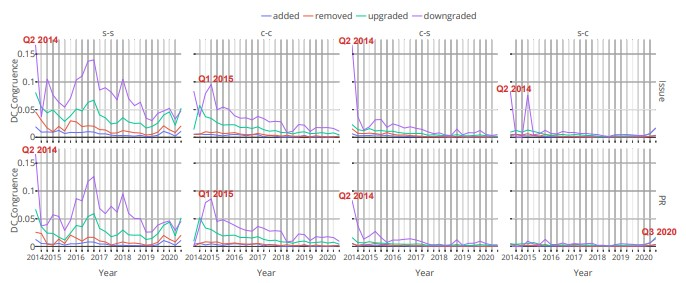
\includegraphics[width=1.1\textwidth]{book/chapter-promisesandperils/pics/congruentViz.jpg}
         \caption{Visualization of a Time analysis for 107,242 libraries.}
     \end{subfigure}
     \begin{subfigure}{0.9\linewidth}
         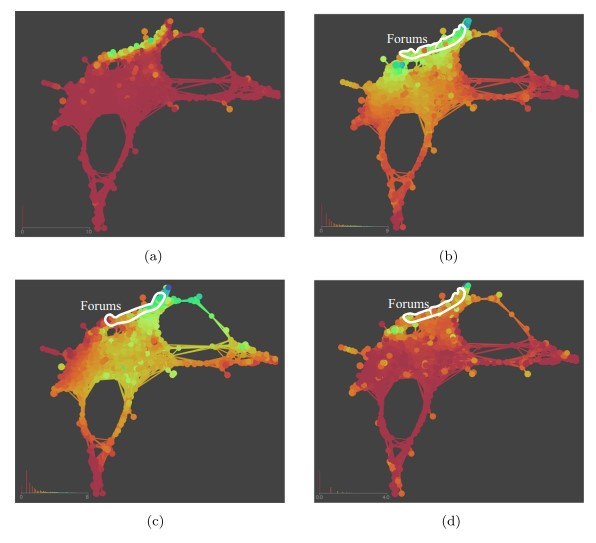
\includegraphics[width=1\textwidth]{book/chapter-promisesandperils/pics/eclipseViz.jpg}
         \caption{A Visual Topology map for 832,058 threads}
     \end{subfigure}
    \caption{Visualisation examples for the two case studies}
    \label{fig:visCase}
\end{figure*}

\smallskip\noindent\textbf{Defining Boundaries}.
The third set of perils (Perils 6-9) is related to the definition of boundaries and completeness and is relevant for both case studies. To mitigate these perils, we recommend the following strategies:

\begin{enumerate}
    \item Researchers should recognise that a dormant project does not necessarily mean that it is inactive. Instead, studies can use alternative heuristics, such as the number of dependents and dependencies, as better indicators of a project's importance in the ecosystem.
    \item Researchers should not rely solely on the programming language to define sub-communities. Using a common package manager for the programming language is a more effective rule of thumb for distinguishing boundaries.
    \item Researchers should avoid random sampling. Instead, sampling should be tailored to the research goals by considering factors such as an appropriate time window or focussing on specific attributes of components (e.g., most dependents, most popular, most contributors).
\end{enumerate}


Peril 6 did not apply to any of the case studies. 
Particularly for the first case, since the goal was to explore the npm package ecosystem, we assumed that the boundaries were clearly defined by the npm registry. 
Similarly, the second case study used the generic Eclipse platform as the boundary. 
Peril 7 was applied to the npm study, while Peril 8 was applied to both case studies. 
As a result, the two cases conducted a qualitative analysis of the dataset to gain deeper insights.
In the first case study, a three-month time window was created to capture dependencies. 
For the second case study, forum contributors were sampled into three groups (i.e., junior, member, or senior) according to the sliding window of their contributions. 

\smallskip\noindent\textbf{Visualisation}.
The final peril (Peril 10) relates to visualisation, which can be challenging due to the vast size and complexity of software ecosystems. As it is not feasible to visualise every aspect of an ecosystem simultaneously, a focused approach is necessary. A mitigation strategy is to select specific attributes of the ecosystem (e.g., the most dependent, most popular, and most contributions) that align with the research needs and objectives. 

Figure \ref{fig:visCase} shows two cases where visualizations are employed to gain insights, especially for large datasets.
In the first figure (a), we visualize the distributions of the data set and applied the appropriate statistical tests, along with the effect size, to test our hypotheses and answer research questions. 
In the second example (b), although not directly related to package ecosystems, the authors utilized a topological visualization \cite{Lum2013ExtractingIF} to gain insights on the over 800,000 forum threads of discussions. 



\section{Chapter Summary}
In this chapter, we explore the various aspects of mining information from the software package ecosystem, presenting three promises and ten perils that researchers should be aware of when undertaking such tasks. The chapter is structured around four key processes for mining: 1) Planning what Information to Mine, 2) Defining Components and their Dependencies, 3) Defining Boundaries and Completeness, and 4) Analysing and Visualising the Data. To help new and experienced researchers navigate these challenges, we introduced the SUG model, which can serve as a valuable tool to minimise threats to validity. Although some perils may be more relevant to specific research objectives, our aim is to equip researchers with the knowledge and resources needed to confidently gather and integrate software package ecosystem data into their work.
%Workflow automation in software development ecosystems (working title)
% %Semantic labeling three-letter-code: WFA (e.g. \chapter{WFA})

% 
\title{Promises and Perils of Mining \\ Software Package Ecosystem Data}
\author{Raula Gaikovina Kula \and Katsuro Inoue \and Christoph Treude}
\institute{Raula Gaikovina Kula \at Nara Institute of Science and Technology, Japan, \email{raula-k@naist.jp}
\and Katsuro Inoue \at Nanzan University, Japan \email{ inoue599@nanzan-u.ac.jp}
\and  Christoph Treude \at The University of Melbourne, Australia \email{christoph.treude@unimelb.edu.au}}

\maketitle
\label{PPM:ch}
\abstract*{The use of third-party packages is becoming increasingly popular and has led to the emergence of large software package ecosystems with a maze of inter-dependencies. Since the reliance on these ecosystems enables developers to reduce development effort and increase productivity, it has attracted the interest of researchers: understanding the infrastructure and dynamics of package ecosystems has given rise to approaches for better code reuse, automated updates, and the avoidance of vulnerabilities, to name a few examples. But the reality of these ecosystems also poses challenges to software engineering researchers, such as: How do we obtain the complete network of dependencies along with the corresponding versioning information? What are the boundaries of these package ecosystem? How do we consistently detect dependencies that are declared but not used? How do we consistently identify developers within a package ecosystem? How much of the ecosystem do we need to understand to analyse a single component? How well do our approaches generalise across different programming languages and package ecosystems? In this chapter, we review promises and perils of mining the rich data related to software package ecosystems available to software engineering researchers.}

\abstract{The use of third-party packages is becoming increasingly popular and has led to the emergence of large software package ecosystems with a maze of inter-dependencies. Since the reliance on these ecosystems enables developers to reduce development effort and increase productivity, it has attracted the interest of researchers: understanding the infrastructure and dynamics of package ecosystems has given rise to approaches for better code reuse, automated updates, and the avoidance of vulnerabilities, to name a few examples. But the reality of these ecosystems also poses challenges to software engineering researchers, such as: How do we obtain the complete network of dependencies along with the corresponding versioning information? What are the boundaries of these package ecosystems? How do we consistently detect dependencies that are declared but not used? How do we consistently identify developers within a package ecosystem? How much of the ecosystem do we need to understand to analyse a single component? How well do our approaches generalise across different programming languages and package ecosystems? In this chapter, we review promises and perils of mining the rich data related to software package ecosystems available to software engineering researchers.}

%%%%%%%%%%%%%%%%%%%%%%%%%%%%%%%%%%%%%%%%%%%%%%%%%%%%%%%%%%%%%%%%%%

\section{Introduction}
\label{PPM:sec:definition}

Third-party libraries are a great way for developers to incorporate code without having to write their own for every functionality required. By using these libraries, developers can save time and energy while still getting the functions they need.
Using third-party libraries is becoming increasingly popular and has led to the emergence of large software package ecosystems such as npm. While these ecosystems offer many benefits, they also come with risks, such as software vulnerability attacks \cite{Chinthanet:ASE2020}.

Large software package ecosystems are a treasure trove for researchers who can investigate a wide range of questions. For example, by studying activity in large ecosystems, researchers can identify which libraries are the most popular and learn what characteristics make them successful \cite{kikas.2017,decan:emse:2019}.
Additionally, research on large ecosystems can help developers understand how to protect their code from malicious actors who may attempt to exploit vulnerabilities or insert malware into popular libraries.
Studying large software package ecosystems can help us better understand the dynamics of open source development in general. Open source development is a complex process that involves many different stakeholders working together (or sometimes competing) to create valuable code that anyone can use or improve upon. By understanding how these interactions play out in different types of ecosystem structures -- including those with many small projects versus few very large ones -- we can develop insights that might be applicable more broadly across other types of collaborative systems.

In this chapter, we identify and discuss promises and perils during the mining process, ranging from planning what information to mine from the ecosystem to analysing and visualising the mined data. 
Therefore, the chapter is broken down into these logical processes of mining ecosystem data: 1) Planning what Information to Mine, 2) Defining Components and their Dependencies, 3) Defining Boundaries and Completeness, and 4) Analysing and Visualising the Data.

This chapter is intended for researchers and practitioners who are interested in exploring and exploiting software package ecosystem information from a diverse range of sources that are publicly available. 
We also highlight the pitfalls to consider during the mining process, particularly when these pitfalls could lead to a misinterpretation of the analysis and results. 
The chapter is written in a manner that encourages newcomers who have little or no experience or who are interested in utilising ecosystem data across different disciplines outside of software engineering.
Our goal is to get new researchers quickly accustomed to gathering ecosystem information for their research.


\section{A Component-based Software Ecosystem}

Defined as a component-based software ecosystem, we suggest using the term `software package ecosystem' as a suitable term for the symbiotic relationships among third-party library components (as software projects or repositories), as these libraries and their dependent clients coexist on the same technological platform, therefore sharing the same environment and other internal and external factors (e.g., security threats, sharing contributions, etc.).
Please refer to the Introduction chapter for an in-depth definition of the different types of software ecosystems.
We present our interpretation of the software package ecosystem in Kula et al.~\cite{KulaSANER18}, where we formally define a package ecosystem using a Software Universe Graph (SUG).
This is modelled as a structured abstraction of the evolution of software systems and their library dependencies over time.

%%%%%%%%%%%%%%%%%%%%%%%%%%%%%%%%%%%%%%%%%%
\begin{figure*}
	\centering
	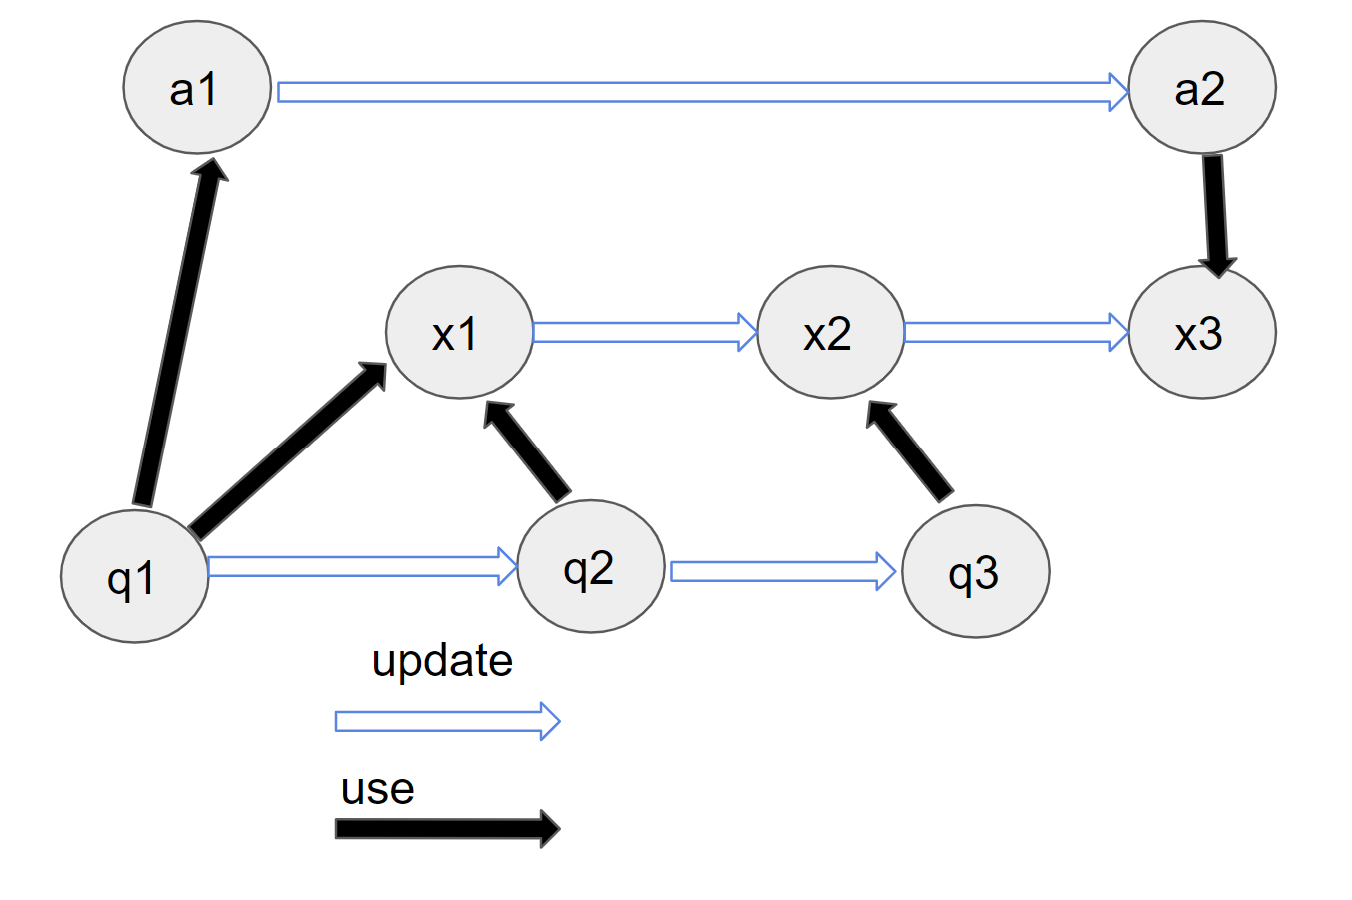
\includegraphics[width=.7\textwidth]{book/chapter-promisesandperils/pics/UniversalExample.jpg}
	\caption{Conceptual example of the Software Universe Graph, depicting the use and update relationships between different software units.}
	\label{fig:SUG}
\end{figure*}
%%%%%%%%%%%%%%%%%%%%%%%%%%%%%%%%%%%%%%%%%%%%%


\paragraph{\textbf{Component-based Representation as a Software Universe Graph}}
\label{PPM:sec:SUG}

First introduced by Kula et al.~\cite{KulaSANER18}, the \textit{Software Universe Graph} (SUG) is a structural abstraction of the software ecosystem of third-party libraries.
Figure \ref{fig:SUG} provides an illustration of the different relationships within the graph.
Let $G= (N,E)$ represent a graph $G$. $N$ is a set of nodes, each node representing a software unit. 
We define a software unit as a version instance of any software program. 

The authors then present the \textit{use} and \textit{update} relationships that exist in the ecosystem.
Hence, the edges $E$ are composed of $E_{use}$ and $E_{update}$. $E_{use}$ is a set of \textit{use-relations} and $E_{update}$ is a set of \textit{update-relations}.

\begin{definition}
An edge $u \rightarrow v \in E_{use}$ means that $u$ uses $v$. The defined functions of $E_{use}$ are:

\begin{equation}
\small
\small \use(u)\equiv \{v|u \rightarrow v\}
\normalsize
\end{equation}
\begin{equation}
\small
\small \useBy(u)\equiv \{v|v \rightarrow u\}
\normalsize
\end{equation}
\end{definition}

Use-relations can be extracted from either the source code or configuration files. 
As shown in Figure \ref{fig:SUG}, node $a1$ uses node $x1$. 
In addition, node $x1$ is used by nodes $a1$, $q1$, and $q2$. Parallel edges for node pairs are not allowed.

\begin{definition}
We represent an update relation from node $a$ to $b$ using $ a \Rightarrow b $, which means that the newer update $b$ was released from node $a$ and is defined as:
\begin{equation}
\small a \Rightarrow b \in E_{update}
\end{equation}
\end{definition}

Update relations refer to when a successive release of a software unit is made available. Figure \ref{fig:SUG} shows that node $q1$ is first updated to node $q2$. Later, node $q2$ is updated to the latest node $q3$. Hence, $q1 \Rightarrow q2 \Rightarrow q3$.
Note that an update should not be confused with forking. 
We distinguish a fork as a separate software unit. 
Each node in the SUG should be denoted by three attributes: \texttt{<name,release,time>}.  
For a node $u$, we define:

\begin{itemize}
	\item \textbf{u.name} Name is the string representation identifier of a software unit.
	We introduce the name axiom: For nodes $u$ and $v$, if $u \Rightarrow v$, then $u.name = v.name$ holds.
	
	\item \textbf{u.release}. Release refers to the specific assigned change reference for a software unit. For nodes $u$ and $v$, if $u \Rightarrow v$
	then $v$ is the immediate successor of $u$. Note that the versioning pattern may vary from project to project. 
	\item \textbf{u.time}. Time refers to the time stamp at which node $u$ was released. For nodes $u$ and $v$ of $u \Rightarrow v$, $u.time < v.time$.
\end{itemize}

\begin{figure}
	\centering
	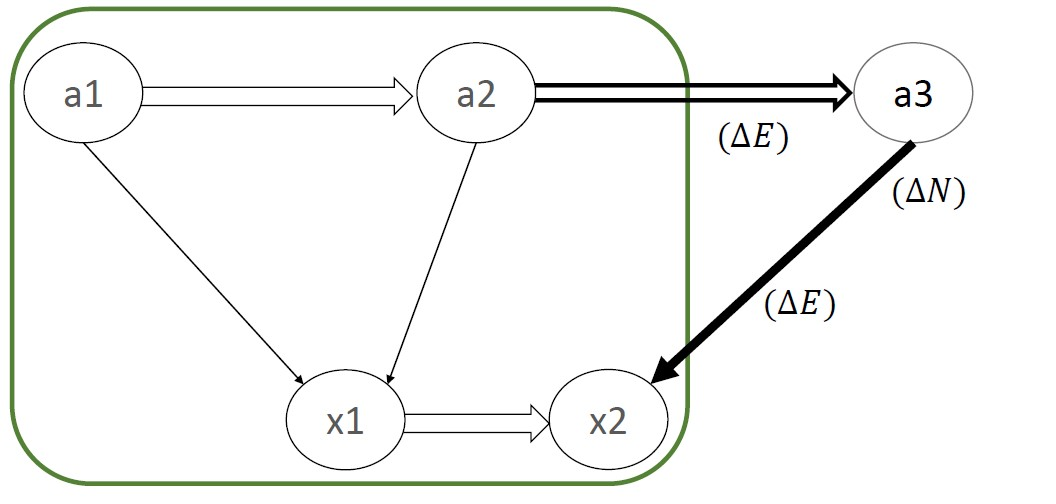
\includegraphics[width=.8\textwidth]{book/chapter-promisesandperils/pics/TemporalSUG.jpg}
	\caption{Temporal property of the SUG}
	\label{fig:SUGTemp}
\end{figure}

\begin{definition}
    
	The SUG has temporal properties.
This describes the simultaneity or ordering in reference to time. Let SUG $G = (N, E) $ be at time $t$. At time $t^{\prime} > t$, we observe an extension of $G$, such that:

\begin{equation}
\small G^{\prime} = (N \cup \Delta N, E \cup \Delta E)
\end{equation}
where $\Delta E \cap (N \times N) = \emptyset$
\end{definition}

Figure \ref{fig:SUGTemp} illustrates the temporal properties of the SUG. 
Here, it is observed that $G'$ is composed of $G$ augmented with newly added node $a3$ and its corresponding $a3 \rightarrow x2$ and $a2 \Rightarrow a3$ relations.
A SUG grows monotonically over time with only additions.
Here, we consider that modification or deletion changes on the SUG do not occur. 

\begin{definition}
    A timed SUG specifies the state of the SUG at any point in time.
So for an SUG $G=(N,E)$, we represent a timed SUG $G_{t}$ at time $t$ as a sub-graph of $G$. Formally,
\begin{equation}
\small G_t\equiv(N_{t}, E_{t})
\end{equation}
where $N_{t} = \{u|u \in N, u.time \leq t \}$ and $E_t = \{ e | e \in E \wedge e \in  N_t \}$
\end{definition}
	


\section{Data Sources}
Researchers can use various datasets to model the ecosystem using the SUG model of usage and update relationships.
The most obvious data source that has revolutionised data mining in the software engineering domain is the GitHub platform. 
Established in 2008, and then purchased by Microsoft in 2020, GitHub is home to various popular Open Source Software. 
GitHub is built on the git version control system and is useful for storing all changes made to a repository. 
In the case of the SUG, a GitHub repository can represent one software unit, whose depend relations can be extracted via a configuration file (such as the package.json file for JavaScript projects).
The repository should also contain the release information that holds the update relations.
Due to its large size, researchers and the GitHub team have made available datasets for researchers to mine, for example through the GitHub API/Graph QL.\footnote{\url{https://docs.github.com/en/graphql}} This is the backend Application Programming Interface (API) that can be used to query large amounts of data on GitHub. Most researchers use the API to download and mine information from the GitHub platform. 
It is important to note that while GitHub introduced a new feature of Dependency Graphs to map the depend relationship,\footnote{\url{https://docs.github.com/en/code-security/supply-chain-security/understanding-your-software-supply-chain/about-the-dependency-graph}} most older projects do not have this feature.
In this case, the researcher would need to manually extract and query the configuration files for dependency information. 

We refer to the first chapter for additional information on data sources for mining software ecosystems. 

\section{Promises and Perils}
\label{PPM:sec:promisesperils}

Using the SUG model of depend and use relations and the available datasets, we can now present our promises and perils of mining ecosystem information.

\subsection{Planning What Information to Mine}

\textbf{Promise 1.}\textit{
Researchers can access and link heterogeneous data related to software package ecosystems, e.g., package registries and bug trackers.}\\

When planning what information to mine from the ecosystem, researchers do not need to limit themselves to the usage and update relationship information.
Platforms that host software repositories include other software management systems such as bug trackers.
For example, GitHub allows researchers to manage GitHub Pull Requests, Issues, and Discussions not only for one project, but for multiple projects.
GitHub provides three management systems that are related to a software repository:

\begin{itemize}
    \item \textit{GitHub Discussions}\footnote{\url{https://docs.github.com/en/discussions}} - The GitHub Discussions forum is a collaborative communication forum for the community around an open source or internal project. Community members can ask and answer questions, share updates, have open-ended conversations, and follow along on decisions affecting the community's way of working.
    \item \textit{GitHub Pull Requests}\footnote{\url{https://docs.github.com/en/pull-requests}} - Pull Requests allow other developers from an ecosystem to make a contribution to a software repository. Pull requests also allow maintainers to discuss and review potential changes with collaborators and add follow-up commits before changes are merged into the software.
    \item \textit{GitHub Issues}\footnote{\url{https://docs.github.com/en/issues}} - Issues are used to track ideas, feedback, tasks, or bugs for work on GitHub.
\end{itemize}

These three systems are examples of how developers contribute to both their own and other projects. 
Hence, to incorporate this information, we can extend the SUG model, creating a model that includes a contribution relationship \cite{wattanakriengkrai2022giving}.

% Note that other platforms may also have management systems, like GitLab, BitBucket and Eclipse.

\begin{definition}
	A Dependency-Contribution graph incorporates contributions by developers whose libraries are involved in dependency relationships. 
\end{definition}

In this work \cite{wattanakriengkrai2022giving}, the authors explore the congruence between dependency updates and developer contributions, based on the original concept of social-technical congruence \cite{stcCataldo2008} where developers contribution patterns are congruent with their coordination needs. Hence, the goal is to identify contributions that are congruent to dependency updates.
As shown in Figure \ref{fig:lib} the authors extend from the typical SUG graph model where $lib_i$ depends (use) on  $lib_k$ and  $lib_j$, while  $lib_j$ also depends on $lib_k$, to the example shown in Figure \ref{fig:dc-graph}.
Different to the SUG, the graph captures developers and their contributions (i.e., the square as $dev_x$ and $dev_y$ represent two different developers making a contribution).
Here contributions are defined as $c$ (Pull Request or Issue) that were submitted to both a library and the client that depends on that library.
Hence, the graph can show contributions that are congruent to dependency changes for a software unit. 

\begin{figure}[t]
     \centering
     \begin{tikzpicture}[
         roundnode/.style={circle, fill=black, minimum size=5mm},
        squarenode/.style={fill=black, text=red, minimum size=5mm},
     ]
    \begin{scope}
         \node[roundnode, label=above:$lib_i$] (s2_proji) at (3, 2.5) {};
        \node[roundnode, label=below:$lib_j$] (s2_projj) at (4,0) {};
         \node[roundnode, label=below:$lib_k$] (s2_projk) at (2,0) {};
     \end{scope}

     \begin{scope} [every edge/.style={draw=gray, very thick}]
         \path [->] (s2_proji) edge (s2_projj);
         \path [->] (s2_proji) edge (s2_projk);
         \path [->] (s2_projj) edge (s2_projk);
     \end{scope}
     \end{tikzpicture}
    
     \caption{Example dependency graph for a given time period}
     \label{fig:lib}
     \vspace{2ex}
 \end{figure}
\begin{figure}[t]
    \centering

    \begin{tikzpicture}[
        roundnode/.style={circle, fill=black, minimum size=5mm},
        squarenode/.style={fill=black, text=red, minimum size=5mm},
    ]
    \begin{scope}
        
        \node[roundnode, label=right:$lib_i$] (s2_proji) at (4, 1.5) {};
        \node[roundnode, label=below:$lib_j$] (s2_projj) at (5,0) {};
        \node[roundnode, label=below:$lib_k$] (s2_projk) at (3,0) {};
        
        \node[squarenode, label=below:$dev_x$] (s3_devx) at (2, 3.5) {};
        
        \node[squarenode, label=below:$dev_y$] (s3_devy) at (6, 3.5) {};
        
    \end{scope}

    \begin{scope} [every edge/.style={draw=gray, very thick}]
        \path [->] (s2_proji)  edge  (s2_projj);
        \path [->] (s2_proji) edge (s2_projk);
        \path [->] (s2_projj) edge (s2_projk);
        
    \end{scope}
    \begin{scope} [every edge/.style={draw=gray, thick, double distance=2pt}]
        \path [->] (6, 2.8) edge node[left = 2mm] {$contribute$} (s2_proji);
        \path [->] (6, 2.8) edge[bend left=15] node[right = 1mm] {$contribute$} (s2_projj);
        \path [->] (2, 2.8) edge node[right = 2mm] {$$} (s2_proji);
        \path [->] (2, 2.8) edge[bend right=15] node[left = 1mm] {$contribute$} (s2_projk);
    \end{scope}
    \end{tikzpicture}
\end{figure}
\begin{figure}[t]
    \centering
    \begin{tikzpicture}[
        roundnode/.style={circle, fill=black, minimum size=5mm},
        squarenode/.style={fill=black, text=red, minimum size=5mm},
    ]
    \end{tikzpicture}
\caption{Example Dependency-Contribution graph showing relationships between contributions and dependencies}
 \label{fig:dc-graph}
\end{figure}

This is just one example of the type of research that is enabled by access to heterogeneous data related to software package ecosystems.

\smallskip\noindent\textbf{Peril 1.}\textit{
 Developers might use different identifiers when contributing to different parts of a software package ecosystem, e.g., when contributing to different libraries.}\\
 
When modelling using such graphs, there is a threat that contributors may use multiple identifiers (i.e., $c_x$ and $c_y$ are the same contributor).
This is a well-known research problem, and there has been work to merge these accounts, such as \cite{wiese2016mailing}.
GitHub has introduced mechanisms such as two-factor authentication\footnote{\url{https://docs.github.com/en/authentication/securing-your-account-with-two-factor-authentication-2fa/configuring-two-factor-authentication}} to counteract the issue of multiple identifiers.
This is since developers might be less likely to switch accounts if it requires cumbersome authentication.


\smallskip\noindent\textbf{Peril 2.}\textit{
Developers' contributions to software package ecosystems might be interspersed with bot contributions, e.g., automated dependency updates.}\\

The rise of automation and artificial intelligence has led to much work on the integration of automated scheduling (i.e., bots) into software development workflows \cite{Storey2016, Farooq2016, Wessel2018, Erlenhov2019, bot_modify_wf} to name a few. These bots are designed to perform specific tasks within a software package ecosystem. For example, a bot may be programmed to automatically update dependencies, test code changes, or deploy software to production. As an example, the Google APIs repo-automation-bots project lists bots for automated labelling of issues and pull requests, automated approval of pull requests, and triggering releases.\footnote{\url{https://github.com/googleapis/repo-automation-bots}}
Bots perform common maintenance tasks in many software projects and are now commonplace \cite{Beschastnikh2017, Urli2018,BIMAN,bot_or_not}.
Especially with bots such as dependabot (automated pull requests to update configurations to reduce the risk of vulnerability threats),\footnote{\url{https://github.com/dependabot}} more and more automation has caused a lot of noise in the contributions between projects.
There are also bots for communication and documentation \cite{Urli2018, Lin2016, Lebeuf2017a}.

To be able to draw accurate conclusions about what humans are doing in software package ecosystems, researchers should consider distinguishing between bot and human contributions.
It is also important to differentiate this from other contributions \cite{maeprasart2022understanding}.
The research community has responded well, with a wide range of techniques and tools to mitigate this peril \cite{Bodegha2021, golzadeh2022accuracy}.

\smallskip\noindent\textbf{Peril 3.}\textit{
Not all developer activities in software package ecosystems are accessible to the public, e.g., library use in proprietary settings.
}\\

Not all developer activities in software package ecosystems are accessible to the public, e.g., when the boundary between open source and industry is blurred \cite{stol2014inner}, which presents a challenge for researchers who aim to study the development process. This is particularly true in proprietary settings where software development is performed behind closed doors or is open source for a limited time period, thus resulting in the artefacts not permanently being publicly available.
This can make it difficult to understand the broader ecosystem in which a software project is developed.
Proprietary settings may lead to non-standardisation in software development practises. Different software projects may use different management systems and tools, making it difficult to accurately compare and analyse software development activities across various projects. For example, some projects may use communication, documentation, and other management tools not captured on the same platform \cite{montgomery2022alternative}. For example, some projects might use Bugzilla instead of issues and pull requests for their bug and code review systems, while others may use Discord, Slack channels, or email threads for their communication needs.

This lack of standardisation in software development practises presents a challenge for researchers who study the software package ecosystem and understand the development process. To address this issue, researchers should strive to collect data from a diverse set of projects to gain a comprehensive understanding of the software package ecosystem. In addition, researchers may need to adjust their methodologies or data collection techniques to accommodate the different tools and practises used by different software projects.

\subsection{Defining Components and their Dependencies}

\smallskip\noindent\textbf{Promise 2.}\textit{
Researchers can access a software package ecosystem's dependency network through package managers and registries, e.g., npm lists the dependencies and dependents for over a million libraries.}\\


With the rise of curated datasets like libraries.io, researchers can now recover and model dependency relations between software units using pre-extracted datasets.
Table \ref{tab:PM_features} shows examples of popular package managers mined from the libraries.io dataset in 2020. 

\begin{table*}[]
\caption{Summary of 13 package managers from libraries.io as ranked by TIOBE in 2020}
 \label{tab:PM_features}
 \centering
\begin{tabular}{@{}llrlll@{}}
\toprule
\begin{tabular}[c]{@{}l@{}}Package \\ Ecosystem\end{tabular} & \begin{tabular}[c]{@{}l@{}}Programming \\ Language\end{tabular} &  \begin{tabular}[c]{@{}l@{}}Tiobe \\ Rank\end{tabular} & Environment & \begin{tabular}[c]{@{}l@{}}Dependency \\ Tree\end{tabular} & \begin{tabular}[c]{@{}l@{}}Package   \\Archive link\end{tabular}\\ \midrule
PyPI & Python & 2 & Python & Flat & pypi.org  \\
Maven & Java & 3 & JVM & Flat & Maven.org  \\
Bower & JavaScript & 7 & Node.js & Flat & bower.io  \\
Meteor & JavaScript & 7 & Node.js & Nested & atmospherejs.com \\
npm & JavaScript & 7 & Node.js & Nested (v2) & npmjs.com  \\
Packagist & PHP & 8 & PHP & Flat & packagist.org \\
Puppet & Ruby & 13 & Ruby MRI & Flat & forge.puppet.com  \\
RubyGems & Ruby & 13 & Ruby MRI & Flat & rubygems.org  \\
CRAN & R & 14 & RStudio & Flat & cran.r-project.org  \\
CPAN & Perl & 15 & Perl & Flat & metacpan.org  \\
GO & Golang & 20 & Go & Flat & pkg.go.dev  \\
NuGet & C\#, VB & 5, 6 & .NET & Flat & nuget.org \\
Anaconda & Python, R, C\# & 2, 14, 5 & Anaconda & Flat & anaconda.org  \\ \bottomrule
\end{tabular}
\end{table*}

\smallskip\noindent\textbf{Peril 4.}\textit{
Different software package ecosystems define the concept of ``dependency'' differently, e.g., by allowing or not allowing different versions of a library on the same dependency tree.
}\\

Different software package ecosystems have varying definitions of what constitutes a dependency. For example, some ecosystems may allow multiple versions of a library to exist on the same dependency tree, while others may restrict developers to a single version of a library \cite{Islam}. These restrictions are often based on the programming language being used, as different languages have different approaches to managing dependencies. It is important to consider the restrictions on dependency relationships when studying software package ecosystems, as they can have a major impact on the development process. For example, the ability to use multiple versions of a library on the same dependency tree can greatly simplify the process of updating dependencies and can make it easier to resolve conflicts between libraries.

One way to visualise the impact of these restrictions is to compare the difference between a nested dependency tree and a directed dependency tree, as shown in Figure \ref{fig:nest}.\footnote{Taken from \url{https://npm.github.io/how-npm-works-docs/npm3/how-npm3-works.html}} This distinction is important because it highlights the different ways that a software unit can depend on different versions of the same library.
In this example, npm v3 creates the dependency tree based on the installation order, therefore flattening unnecessary nested dependencies (i.e., B v1.0 in cyan). This reduces the complexity of a nested tree by resolving some of the transitive dependencies (nested dependencies).

\begin{figure}
	\centering
	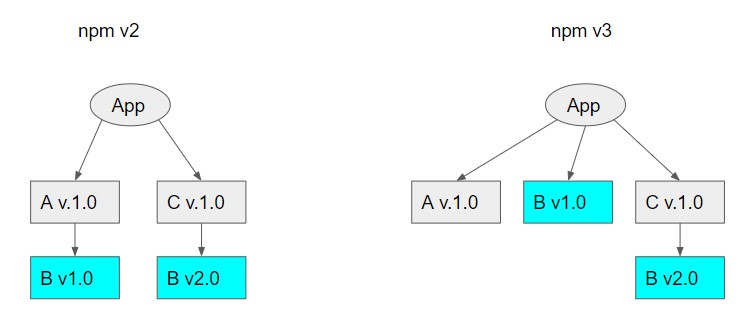
\includegraphics[width=.8\textwidth]{book/chapter-promisesandperils/pics/nestedv2.jpg}
	\caption{Difference between flat and nested dependencies}
	\label{fig:nest}
\end{figure}

\smallskip\noindent\textbf{Peril 5.}\textit{
Developers might declare a dependency to other parts of a software package ecosystem but not use it, e.g., because they failed to update its removal.
}\\

It is common for developers to declare dependencies on other parts of the software package ecosystem but not always use them. This can happen for various reasons, such as forgetting to remove the dependency after it is no longer needed. This can pose a challenge for researchers who are trying to extract dependencies from package managers, like those in configuration files, as there may be inconsistencies between the listed dependencies and what is actually being compiled and used by the code. This can lead to a biased understanding of the software package ecosystem and the relationships between software components.

To address this issue, there have been numerous efforts to track the actual library dependencies compiled and executed in software systems. These efforts aim to provide a more accurate understanding of the dependencies and the relationships between software components. For example, research has been conducted on the use of dynamic analysis to track compiled dependencies in real time and on the development of tools to automatically detect and track executed dependencies \cite{Zapata:ICSME2018, Ponta2018,Chinthanet:ASE2020}.

\subsection{Defining Boundaries and Completeness}

\smallskip\noindent\textbf{Promise 3.}\textit{
Researchers can use the boundaries of software package ecosystems to study communities of developers, e.g., developers contributing to and/or benefiting from the npm ecosystem.
}\\

Following Promise 2, the emergence of package managers has also led to studies that approximate software communities.
Using the libraries.io dataset, researchers were able to study projects that host libraries that use package managers.
Researchers have used this dataset to compare different library ecosystems \cite{kikas.2017,decan:emse:2019,CogoDown2019}.


\smallskip\noindent\textbf{Peril 6.}\textit{
Package managers do not always represent software package ecosystems, their communities, or their sub-communities, e.g., in cases where multiple package managers exist.
}\\

Package managers are a fundamental aspect of software package ecosystems, but do not always fully represent the complex relationships and interactions that occur within a community of developers and users, as shown in Table~\ref{tab:PM_features}. In some cases, multiple package managers exist for the same programming language, creating a complex landscape of software libraries and dependencies that are not always easily understood. For instance, Bower and Meteor manage npm libraries, which can lead to confusion and overlap in the management of dependencies.

Similarly, Java, Scala, Android, and other Java-based open source communities all use the Maven package manager, but each of these communities has its own unique set of libraries, dependencies, and development practises. Researchers should be aware of the limitations of package managers when studying software package ecosystems, and consider the broader context and relationships that exist within these communities. 

\smallskip\noindent\textbf{Peril 7.}\textit{
Lack of activity in parts of a software package ecosystem does not necessarily indicate project failure, e.g., when highly depended-upon libraries are feature-complete.
}\\

It is important to note that lack of activity in a part of a software package ecosystem does not always mean project failure \cite{coelho2017modern}. In some cases, highly relied-upon libraries that have reached feature-completeness may see little activity, but continue to be used by the software community. 

However, it is still important to consider the long-term sustainability of these libraries, especially given the rate at which technology and software development practises change. This has become a topic of interest in recent years, and researchers have explored best practises for sustaining open source projects and ensuring their continued success \cite{Ait2022,valiev2018ecosystem}. Understanding the factors that contribute to project sustainability is important to ensure the longevity and continued growth of software package ecosystems.

\smallskip\noindent\textbf{Peril 8.}\textit{
Sampling from a software package ecosystem is challenging since sub-setting might alter the dependency network, e.g., by breaking dependency chains.
}\\

Sampling from a package ecosystem is not straightforward, as the sample composition can be significantly affected due to missing dependency links between libraries. For instance, a subset of the ecosystem might alter the dependencies between libraries, leading to the breakdown of the dependency chains. This could lead to an incomplete picture of the software package ecosystem, leading to incorrect conclusions from a study. To minimise this risk, researchers should carefully consider the boundaries of their study and choose the appropriate sampling method based on the research questions and goals. For example, researchers could focus on popular, highly dependent, or risk-vulnerable aspects of the ecosystem as a starting point. 
For some ecosystems, the number of downloads, GitHub stars, and watchers are other aspects for the researcher to utilise.


\smallskip\noindent\textbf{Peril 9.}\textit{
Sampling from a software package ecosystem is challenging since the dependency network changes over time, e.g., when dependencies are added, removed, upgraded, or downgraded.
}\\

The dynamic nature of package ecosystems and the constant changes to their dependencies can impact the generalisability of the results. Therefore, it is important to also consider the time granularity of the analysis. For example, if the goal is to understand the evolution of dependencies over time, a finer time granularity may be necessary to capture the smaller changes and trends. However, if the goal is to understand the overall structure and relationships within the ecosystem, a coarser time granularity may be sufficient. Based on recent studies \cite{wattanakriengkrai2022giving,valiev2018ecosystem,Mirsaeedi:icse2020, Brindescu:emse2020, Nassif:icsme2017}, a three-month window seems appropriate for some studies.
Another level of granularity to consider is the size of the component. For instance, there are cases where a single package may contain more than one repository, especially for large library frameworks. 
The granularity also depends on the nature of the ecosystem itself. For instance, researchers should understand whether the ecosystem comprises library packages (e.g., PyPI), plugins (e.g., Eclipse), or is a library distribution (e.g., Android).



\subsection{Analysing and Visualising the Data}

\textbf{Peril 10.}\textit{
Analysing and visualising entire software package ecosystems is challenging due to their size, e.g., in terms of nodes and edges in the network.
}\\

The size of software package ecosystems implies large data sets, which can be overwhelming for tools and algorithms to analyse and display. Therefore, it may be necessary to make choices about the granularity of the data included in the analysis and visualisation. Another alternative is to focus on the most critical parts of the software package ecosystem, such as the high-level structure, highly dependent packages, or parts of the system that pose a risk to security and reliability. 
The key is to strike a balance between detail and simplicity, providing a meaningful representation of the ecosystem while being able to handle the complexity of its size.


\section{Application: When to Apply Which Peril}
\label{PPM:sec:application}

We include a disclaimer stating that not all perils are applicable to every mining situation. To demonstrate the practical application of our perils and their mitigation, we present two case studies that involve mining the software package ecosystem. Each case study has a distinct research objective and focusses on a specific dataset to be mined.

\subsection{Two Case Studies}
Table \ref{tab:cases} presents the two case studies we have selected for this analysis.
The \textit{first case} involves mining for contributions congruent to dependency updates \cite{wattanakriengkrai2022giving}. 
In this work, the authors mine GitHub repositories for Pull Requests and Issues that were submitted and merged congruent to dependency updates within the npm ecosystem. 
The \textit{second case} involves mining communication data for the Eclipse ecosystem \cite{Nugroho2021}. Although the second case does not mine for dependency relations (i.e., use relations),  we show that these perils still apply when mining for other relationships in an ecosystem.
Moreover, the second case studies the Eclipse ecosystem, which is a different dataset compared to the more popular GitHub dataset.

\subsection{Applying Perils and their Mitigation Strategies}
Table \ref{tab:perilsapp} provides a summary of the perils that can be applied to each of the case studies. We will now go into the details of mitigation strategies based on these perils. 
For better organisation and understanding, we have grouped the perils according to the four logical processes for mining.

\smallskip\noindent\textbf{Information to Mine}. 
The first set of mitigation strategies, which addresses perils 1-3, focusses on planning which information to mine. There are two primary strategies that researchers can employ:


\begin{enumerate}
    \item Researchers should use research tools and techniques to remove noise and other biases in the dataset, such as bot detection and the handling of multiple identities. This strategy was implemented in both case studies, as contributions and discussions often have the potential to involve bots or developers with multiple identities.
\item Depending on the research goals, researchers should recognise that not all contributions are equal and filter the dataset accordingly.
\end{enumerate}

We applied these two strategies to both cases. In the first case, the goal was to capture all congruent contributions, so we filtered out contributions made to libraries without dependencies. Since all npm packages are listed in the registry, Peril 3 (private activities) did not apply.
In the second case, we addressed Peril 1 by conducting a qualitative analysis to ensure that the member identities were not duplicated, as Eclipse developers were known to change identities. To mitigate Peril 2, we removed bot responses. For the second case, since all forum data is made public, Peril 3 did not apply.


\begin{table}
\centering
\caption{Description of the research objectives and datasets for the case studies}
 \label{tab:cases}
\begin{tabular}{lp{5cm}r} 
\toprule
\textbf{Case Study} & \textbf{Research Objective}                                                          & \textbf{Datasets}           \\
\midrule
Wattanakriengkrai \etal \cite{wattanakriengkrai2022giving}             & Explore code contributions between library and client (i.e, use-relations)  & libraries.io\\
& &  GitHub API \\
Nugroho \etal \cite{Nugroho2021}                & Explore discussion contributions between contributors (i.e., contributions) & Eclipse API                \\
\bottomrule
\end{tabular}
\end{table}

\begin{table}
\centering
\caption{Application of each peril to the case studies}
 \label{tab:perilsapp}
\begin{tabular}{rp{8cm}ccc} 
\toprule                   
& \textbf{Perils}       & case 1      & case 2                 \\
                                                                               & & npm  & Eclipse   \\
\midrule
\textbf{P1} &Developers might use different identifiers when contributing to different parts of a software package ecosystem, e.g., when contributing to different libraries.                             &    \CheckedBox         &          \CheckedBox           \\ 
%\hline
\textbf{P2} & Developers' contributions to software package ecosystems might be interspersed with bot contributions, e.g., automated dependency updates.                                                      &      \CheckedBox               &      \CheckedBox               \\ 
%\hline
\textbf{P3} & Not all developer activities in software package ecosystems are accessible to the public, e.g., library use in proprietary settings.                                                         &         -           &      \CheckedBox               \\ 
%\hline
\textbf{P4} & Different software package ecosystems define the concept of \`{}\`{}dependency'' differently, e.g., by allowing or not allowing different versions of a library on the same dependency tree. &         \CheckedBox       &     -                            \\ 
%\hline
\textbf{P5} & Developers might declare a dependency to other parts of a software package ecosystem but not use it, e.g., because they failed to update its removal.                                        &     -           &  -    \\
%\hline
\textbf{P6} &Package managers do not always represent software package ecosystems, their communities, or their sub-communities, e.g., in cases where multiple package managers exist.                     &     -                   &  -                  \\
%\hline
\textbf{P7} & Lack of activity in parts of a software package ecosystem does not necessarily indicate project failure, e.g., when highly depended-upon libraries are feature-complete.                     &       \CheckedBox         &  -                           \\
%\hline
\textbf{P8} &Sampling from a software package ecosystem is challenging since sub-setting might alter the dependency network, e.g., by breaking dependency chains.                                         &        \CheckedBox        &     \CheckedBox                                \\
%\hline
\textbf{P9} &Sampling from a software package ecosystem is challenging since the dependency network changes over time, e.g., when dependencies are added, removed, upgraded, or downgraded.               &       \CheckedBox         &     -                          \\
%\hline
\textbf{P10} &Analysing and visualising entire software package ecosystems is challenging due to their size, e.g., in terms of nodes and edges in the network.                                  &        \CheckedBox      &      \CheckedBox               \\
\bottomrule
\end{tabular}
\end{table}

\smallskip\noindent\textbf{Defining Dependencies}. 
The second set of perils (Perils 4-5) is related to dependency relationships between software units, and only the first case study is applicable. To address these perils, researchers should adopt the following strategy:

\begin{enumerate}
    \item Researchers should not rely solely on listed dependencies in configuration files (e.g., pom.xml, package.json, etc.) as a measure of dependency between two components. Instead, code-centric approaches should be used to validate which libraries are actually depended upon.
\end{enumerate}

For example, in the first case, in addition to mining the configuration information, the authors also analysed the similarity of the source code contributions to address Peril 4. Regarding Peril 5, since the study's objective was to investigate changes to the configuration files, the risk of the update not being executed was deemed less important.
It is important to note that the second case study did not include dependency analysis and, therefore, these perils did not apply.

\begin{figure*}[]
    \centering
    \begin{subfigure}{0.9\linewidth}
         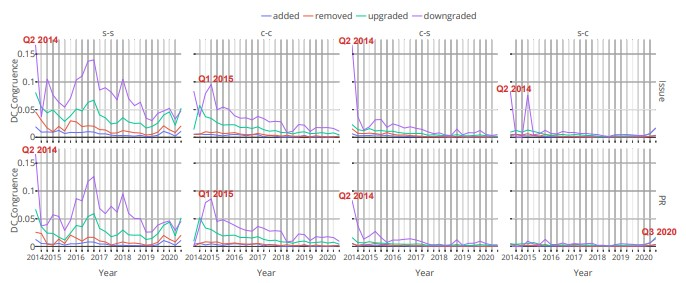
\includegraphics[width=1.1\textwidth]{book/chapter-promisesandperils/pics/congruentViz.jpg}
         \caption{Visualization of a Time analysis for 107,242 libraries.}
     \end{subfigure}
     \begin{subfigure}{0.9\linewidth}
         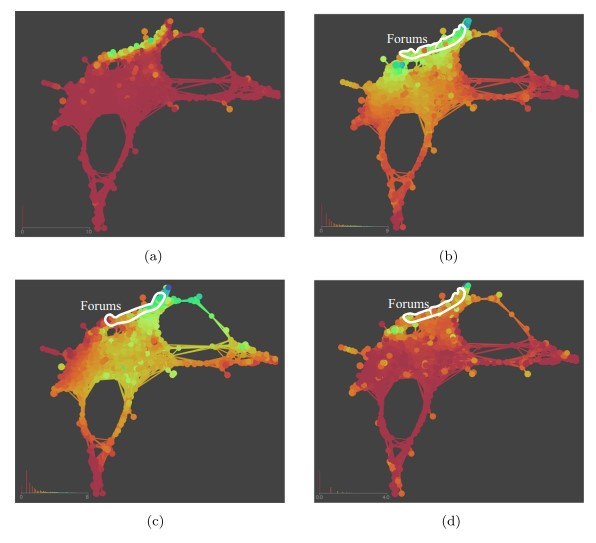
\includegraphics[width=1\textwidth]{book/chapter-promisesandperils/pics/eclipseViz.jpg}
         \caption{A Visual Topology map for 832,058 threads}
     \end{subfigure}
    \caption{Visualisation examples for the two case studies}
    \label{fig:visCase}
\end{figure*}

\smallskip\noindent\textbf{Defining Boundaries}.
The third set of perils (Perils 6-9) is related to the definition of boundaries and completeness and is relevant for both case studies. To mitigate these perils, we recommend the following strategies:

\begin{enumerate}
    \item Researchers should recognise that a dormant project does not necessarily mean that it is inactive. Instead, studies can use alternative heuristics, such as the number of dependents and dependencies, as better indicators of a project's importance in the ecosystem.
    \item Researchers should not rely solely on the programming language to define sub-communities. Using a common package manager for the programming language is a more effective rule of thumb for distinguishing boundaries.
    \item Researchers should avoid random sampling. Instead, sampling should be tailored to the research goals by considering factors such as an appropriate time window or focussing on specific attributes of components (e.g., most dependents, most popular, most contributors).
\end{enumerate}


Peril 6 did not apply to any of the case studies. 
Particularly for the first case, since the goal was to explore the npm package ecosystem, we assumed that the boundaries were clearly defined by the npm registry. 
Similarly, the second case study used the generic Eclipse platform as the boundary. 
Peril 7 was applied to the npm study, while Peril 8 was applied to both case studies. 
As a result, the two cases conducted a qualitative analysis of the dataset to gain deeper insights.
In the first case study, a three-month time window was created to capture dependencies. 
For the second case study, forum contributors were sampled into three groups (i.e., junior, member, or senior) according to the sliding window of their contributions. 

\smallskip\noindent\textbf{Visualisation}.
The final peril (Peril 10) relates to visualisation, which can be challenging due to the vast size and complexity of software ecosystems. As it is not feasible to visualise every aspect of an ecosystem simultaneously, a focused approach is necessary. A mitigation strategy is to select specific attributes of the ecosystem (e.g., the most dependent, most popular, and most contributions) that align with the research needs and objectives. 

Figure \ref{fig:visCase} shows two cases where visualizations are employed to gain insights, especially for large datasets.
In the first figure (a), we visualize the distributions of the data set and applied the appropriate statistical tests, along with the effect size, to test our hypotheses and answer research questions. 
In the second example (b), although not directly related to package ecosystems, the authors utilized a topological visualization \cite{Lum2013ExtractingIF} to gain insights on the over 800,000 forum threads of discussions. 



\section{Chapter Summary}
In this chapter, we explore the various aspects of mining information from the software package ecosystem, presenting three promises and ten perils that researchers should be aware of when undertaking such tasks. The chapter is structured around four key processes for mining: 1) Planning what Information to Mine, 2) Defining Components and their Dependencies, 3) Defining Boundaries and Completeness, and 4) Analysing and Visualising the Data. To help new and experienced researchers navigate these challenges, we introduced the SUG model, which can serve as a valuable tool to minimise threats to validity. Although some perils may be more relevant to specific research objectives, our aim is to equip researchers with the knowledge and resources needed to confidently gather and integrate software package ecosystem data into their work.
 %Analysing Infrastructure-as-Code Ecosystems
% %Semantic labeling three-letter-code: IAC (e.g. \chapter{IAC})

% %%%%%%%%%%%%%%%%%%%%%part.tex%%%%%%%%%%%%%%%%%%%%%%%%%%%%%%%%%%
% 
% sample part title
%
% Use this file as a template for your own input.
%
%%%%%%%%%%%%%%%%%%%%%%%% Springer %%%%%%%%%%%%%%%%%%%%%%%%%%

\begin{partbacktext}
\part{MODEL-CENTERED SOFTWARE ECOSYSTEMS}
\label{part:models}

\end{partbacktext} %MODEL-CENTERED SOFTWARE ECOSYSTEMS
% 
\title{Promises and Perils of Mining \\ Software Package Ecosystem Data}
\author{Raula Gaikovina Kula \and Katsuro Inoue \and Christoph Treude}
\institute{Raula Gaikovina Kula \at Nara Institute of Science and Technology, Japan, \email{raula-k@naist.jp}
\and Katsuro Inoue \at Nanzan University, Japan \email{ inoue599@nanzan-u.ac.jp}
\and  Christoph Treude \at The University of Melbourne, Australia \email{christoph.treude@unimelb.edu.au}}

\maketitle
\label{PPM:ch}
\abstract*{The use of third-party packages is becoming increasingly popular and has led to the emergence of large software package ecosystems with a maze of inter-dependencies. Since the reliance on these ecosystems enables developers to reduce development effort and increase productivity, it has attracted the interest of researchers: understanding the infrastructure and dynamics of package ecosystems has given rise to approaches for better code reuse, automated updates, and the avoidance of vulnerabilities, to name a few examples. But the reality of these ecosystems also poses challenges to software engineering researchers, such as: How do we obtain the complete network of dependencies along with the corresponding versioning information? What are the boundaries of these package ecosystem? How do we consistently detect dependencies that are declared but not used? How do we consistently identify developers within a package ecosystem? How much of the ecosystem do we need to understand to analyse a single component? How well do our approaches generalise across different programming languages and package ecosystems? In this chapter, we review promises and perils of mining the rich data related to software package ecosystems available to software engineering researchers.}

\abstract{The use of third-party packages is becoming increasingly popular and has led to the emergence of large software package ecosystems with a maze of inter-dependencies. Since the reliance on these ecosystems enables developers to reduce development effort and increase productivity, it has attracted the interest of researchers: understanding the infrastructure and dynamics of package ecosystems has given rise to approaches for better code reuse, automated updates, and the avoidance of vulnerabilities, to name a few examples. But the reality of these ecosystems also poses challenges to software engineering researchers, such as: How do we obtain the complete network of dependencies along with the corresponding versioning information? What are the boundaries of these package ecosystems? How do we consistently detect dependencies that are declared but not used? How do we consistently identify developers within a package ecosystem? How much of the ecosystem do we need to understand to analyse a single component? How well do our approaches generalise across different programming languages and package ecosystems? In this chapter, we review promises and perils of mining the rich data related to software package ecosystems available to software engineering researchers.}

%%%%%%%%%%%%%%%%%%%%%%%%%%%%%%%%%%%%%%%%%%%%%%%%%%%%%%%%%%%%%%%%%%

\section{Introduction}
\label{PPM:sec:definition}

Third-party libraries are a great way for developers to incorporate code without having to write their own for every functionality required. By using these libraries, developers can save time and energy while still getting the functions they need.
Using third-party libraries is becoming increasingly popular and has led to the emergence of large software package ecosystems such as npm. While these ecosystems offer many benefits, they also come with risks, such as software vulnerability attacks \cite{Chinthanet:ASE2020}.

Large software package ecosystems are a treasure trove for researchers who can investigate a wide range of questions. For example, by studying activity in large ecosystems, researchers can identify which libraries are the most popular and learn what characteristics make them successful \cite{kikas.2017,decan:emse:2019}.
Additionally, research on large ecosystems can help developers understand how to protect their code from malicious actors who may attempt to exploit vulnerabilities or insert malware into popular libraries.
Studying large software package ecosystems can help us better understand the dynamics of open source development in general. Open source development is a complex process that involves many different stakeholders working together (or sometimes competing) to create valuable code that anyone can use or improve upon. By understanding how these interactions play out in different types of ecosystem structures -- including those with many small projects versus few very large ones -- we can develop insights that might be applicable more broadly across other types of collaborative systems.

In this chapter, we identify and discuss promises and perils during the mining process, ranging from planning what information to mine from the ecosystem to analysing and visualising the mined data. 
Therefore, the chapter is broken down into these logical processes of mining ecosystem data: 1) Planning what Information to Mine, 2) Defining Components and their Dependencies, 3) Defining Boundaries and Completeness, and 4) Analysing and Visualising the Data.

This chapter is intended for researchers and practitioners who are interested in exploring and exploiting software package ecosystem information from a diverse range of sources that are publicly available. 
We also highlight the pitfalls to consider during the mining process, particularly when these pitfalls could lead to a misinterpretation of the analysis and results. 
The chapter is written in a manner that encourages newcomers who have little or no experience or who are interested in utilising ecosystem data across different disciplines outside of software engineering.
Our goal is to get new researchers quickly accustomed to gathering ecosystem information for their research.


\section{A Component-based Software Ecosystem}

Defined as a component-based software ecosystem, we suggest using the term `software package ecosystem' as a suitable term for the symbiotic relationships among third-party library components (as software projects or repositories), as these libraries and their dependent clients coexist on the same technological platform, therefore sharing the same environment and other internal and external factors (e.g., security threats, sharing contributions, etc.).
Please refer to the Introduction chapter for an in-depth definition of the different types of software ecosystems.
We present our interpretation of the software package ecosystem in Kula et al.~\cite{KulaSANER18}, where we formally define a package ecosystem using a Software Universe Graph (SUG).
This is modelled as a structured abstraction of the evolution of software systems and their library dependencies over time.

%%%%%%%%%%%%%%%%%%%%%%%%%%%%%%%%%%%%%%%%%%
\begin{figure*}
	\centering
	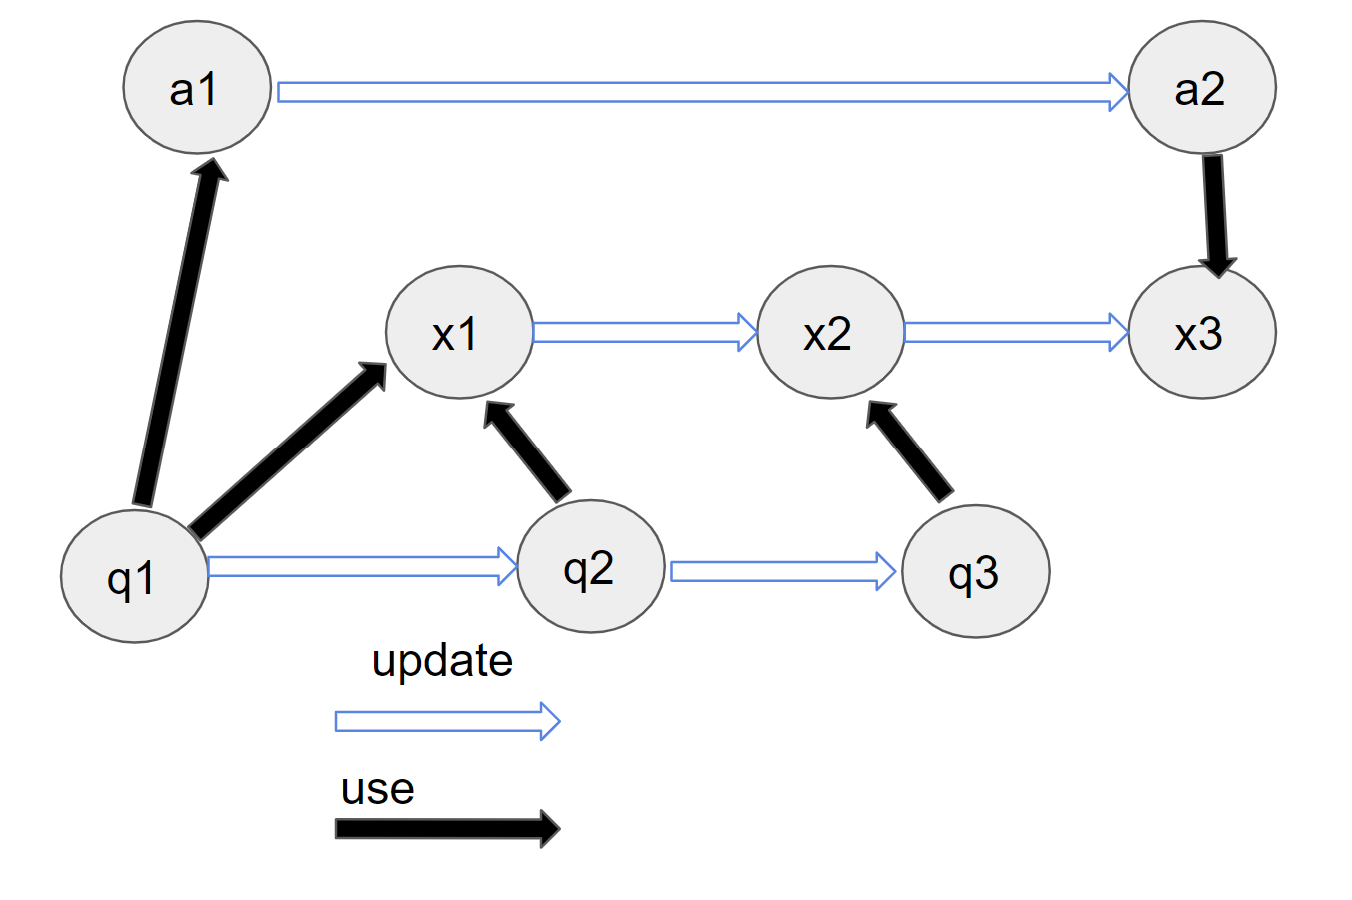
\includegraphics[width=.7\textwidth]{book/chapter-promisesandperils/pics/UniversalExample.jpg}
	\caption{Conceptual example of the Software Universe Graph, depicting the use and update relationships between different software units.}
	\label{fig:SUG}
\end{figure*}
%%%%%%%%%%%%%%%%%%%%%%%%%%%%%%%%%%%%%%%%%%%%%


\paragraph{\textbf{Component-based Representation as a Software Universe Graph}}
\label{PPM:sec:SUG}

First introduced by Kula et al.~\cite{KulaSANER18}, the \textit{Software Universe Graph} (SUG) is a structural abstraction of the software ecosystem of third-party libraries.
Figure \ref{fig:SUG} provides an illustration of the different relationships within the graph.
Let $G= (N,E)$ represent a graph $G$. $N$ is a set of nodes, each node representing a software unit. 
We define a software unit as a version instance of any software program. 

The authors then present the \textit{use} and \textit{update} relationships that exist in the ecosystem.
Hence, the edges $E$ are composed of $E_{use}$ and $E_{update}$. $E_{use}$ is a set of \textit{use-relations} and $E_{update}$ is a set of \textit{update-relations}.

\begin{definition}
An edge $u \rightarrow v \in E_{use}$ means that $u$ uses $v$. The defined functions of $E_{use}$ are:

\begin{equation}
\small
\small \use(u)\equiv \{v|u \rightarrow v\}
\normalsize
\end{equation}
\begin{equation}
\small
\small \useBy(u)\equiv \{v|v \rightarrow u\}
\normalsize
\end{equation}
\end{definition}

Use-relations can be extracted from either the source code or configuration files. 
As shown in Figure \ref{fig:SUG}, node $a1$ uses node $x1$. 
In addition, node $x1$ is used by nodes $a1$, $q1$, and $q2$. Parallel edges for node pairs are not allowed.

\begin{definition}
We represent an update relation from node $a$ to $b$ using $ a \Rightarrow b $, which means that the newer update $b$ was released from node $a$ and is defined as:
\begin{equation}
\small a \Rightarrow b \in E_{update}
\end{equation}
\end{definition}

Update relations refer to when a successive release of a software unit is made available. Figure \ref{fig:SUG} shows that node $q1$ is first updated to node $q2$. Later, node $q2$ is updated to the latest node $q3$. Hence, $q1 \Rightarrow q2 \Rightarrow q3$.
Note that an update should not be confused with forking. 
We distinguish a fork as a separate software unit. 
Each node in the SUG should be denoted by three attributes: \texttt{<name,release,time>}.  
For a node $u$, we define:

\begin{itemize}
	\item \textbf{u.name} Name is the string representation identifier of a software unit.
	We introduce the name axiom: For nodes $u$ and $v$, if $u \Rightarrow v$, then $u.name = v.name$ holds.
	
	\item \textbf{u.release}. Release refers to the specific assigned change reference for a software unit. For nodes $u$ and $v$, if $u \Rightarrow v$
	then $v$ is the immediate successor of $u$. Note that the versioning pattern may vary from project to project. 
	\item \textbf{u.time}. Time refers to the time stamp at which node $u$ was released. For nodes $u$ and $v$ of $u \Rightarrow v$, $u.time < v.time$.
\end{itemize}

\begin{figure}
	\centering
	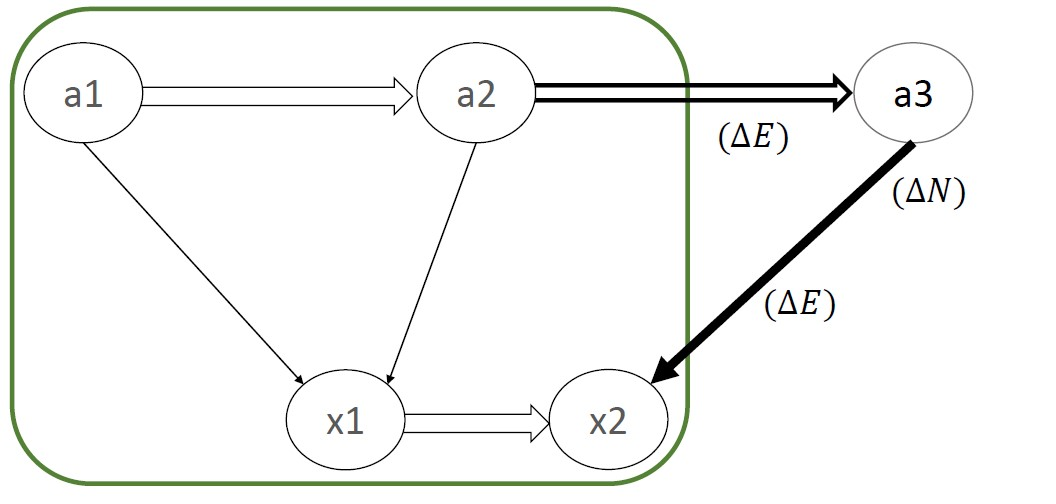
\includegraphics[width=.8\textwidth]{book/chapter-promisesandperils/pics/TemporalSUG.jpg}
	\caption{Temporal property of the SUG}
	\label{fig:SUGTemp}
\end{figure}

\begin{definition}
    
	The SUG has temporal properties.
This describes the simultaneity or ordering in reference to time. Let SUG $G = (N, E) $ be at time $t$. At time $t^{\prime} > t$, we observe an extension of $G$, such that:

\begin{equation}
\small G^{\prime} = (N \cup \Delta N, E \cup \Delta E)
\end{equation}
where $\Delta E \cap (N \times N) = \emptyset$
\end{definition}

Figure \ref{fig:SUGTemp} illustrates the temporal properties of the SUG. 
Here, it is observed that $G'$ is composed of $G$ augmented with newly added node $a3$ and its corresponding $a3 \rightarrow x2$ and $a2 \Rightarrow a3$ relations.
A SUG grows monotonically over time with only additions.
Here, we consider that modification or deletion changes on the SUG do not occur. 

\begin{definition}
    A timed SUG specifies the state of the SUG at any point in time.
So for an SUG $G=(N,E)$, we represent a timed SUG $G_{t}$ at time $t$ as a sub-graph of $G$. Formally,
\begin{equation}
\small G_t\equiv(N_{t}, E_{t})
\end{equation}
where $N_{t} = \{u|u \in N, u.time \leq t \}$ and $E_t = \{ e | e \in E \wedge e \in  N_t \}$
\end{definition}
	


\section{Data Sources}
Researchers can use various datasets to model the ecosystem using the SUG model of usage and update relationships.
The most obvious data source that has revolutionised data mining in the software engineering domain is the GitHub platform. 
Established in 2008, and then purchased by Microsoft in 2020, GitHub is home to various popular Open Source Software. 
GitHub is built on the git version control system and is useful for storing all changes made to a repository. 
In the case of the SUG, a GitHub repository can represent one software unit, whose depend relations can be extracted via a configuration file (such as the package.json file for JavaScript projects).
The repository should also contain the release information that holds the update relations.
Due to its large size, researchers and the GitHub team have made available datasets for researchers to mine, for example through the GitHub API/Graph QL.\footnote{\url{https://docs.github.com/en/graphql}} This is the backend Application Programming Interface (API) that can be used to query large amounts of data on GitHub. Most researchers use the API to download and mine information from the GitHub platform. 
It is important to note that while GitHub introduced a new feature of Dependency Graphs to map the depend relationship,\footnote{\url{https://docs.github.com/en/code-security/supply-chain-security/understanding-your-software-supply-chain/about-the-dependency-graph}} most older projects do not have this feature.
In this case, the researcher would need to manually extract and query the configuration files for dependency information. 

We refer to the first chapter for additional information on data sources for mining software ecosystems. 

\section{Promises and Perils}
\label{PPM:sec:promisesperils}

Using the SUG model of depend and use relations and the available datasets, we can now present our promises and perils of mining ecosystem information.

\subsection{Planning What Information to Mine}

\textbf{Promise 1.}\textit{
Researchers can access and link heterogeneous data related to software package ecosystems, e.g., package registries and bug trackers.}\\

When planning what information to mine from the ecosystem, researchers do not need to limit themselves to the usage and update relationship information.
Platforms that host software repositories include other software management systems such as bug trackers.
For example, GitHub allows researchers to manage GitHub Pull Requests, Issues, and Discussions not only for one project, but for multiple projects.
GitHub provides three management systems that are related to a software repository:

\begin{itemize}
    \item \textit{GitHub Discussions}\footnote{\url{https://docs.github.com/en/discussions}} - The GitHub Discussions forum is a collaborative communication forum for the community around an open source or internal project. Community members can ask and answer questions, share updates, have open-ended conversations, and follow along on decisions affecting the community's way of working.
    \item \textit{GitHub Pull Requests}\footnote{\url{https://docs.github.com/en/pull-requests}} - Pull Requests allow other developers from an ecosystem to make a contribution to a software repository. Pull requests also allow maintainers to discuss and review potential changes with collaborators and add follow-up commits before changes are merged into the software.
    \item \textit{GitHub Issues}\footnote{\url{https://docs.github.com/en/issues}} - Issues are used to track ideas, feedback, tasks, or bugs for work on GitHub.
\end{itemize}

These three systems are examples of how developers contribute to both their own and other projects. 
Hence, to incorporate this information, we can extend the SUG model, creating a model that includes a contribution relationship \cite{wattanakriengkrai2022giving}.

% Note that other platforms may also have management systems, like GitLab, BitBucket and Eclipse.

\begin{definition}
	A Dependency-Contribution graph incorporates contributions by developers whose libraries are involved in dependency relationships. 
\end{definition}

In this work \cite{wattanakriengkrai2022giving}, the authors explore the congruence between dependency updates and developer contributions, based on the original concept of social-technical congruence \cite{stcCataldo2008} where developers contribution patterns are congruent with their coordination needs. Hence, the goal is to identify contributions that are congruent to dependency updates.
As shown in Figure \ref{fig:lib} the authors extend from the typical SUG graph model where $lib_i$ depends (use) on  $lib_k$ and  $lib_j$, while  $lib_j$ also depends on $lib_k$, to the example shown in Figure \ref{fig:dc-graph}.
Different to the SUG, the graph captures developers and their contributions (i.e., the square as $dev_x$ and $dev_y$ represent two different developers making a contribution).
Here contributions are defined as $c$ (Pull Request or Issue) that were submitted to both a library and the client that depends on that library.
Hence, the graph can show contributions that are congruent to dependency changes for a software unit. 

\begin{figure}[t]
     \centering
     \begin{tikzpicture}[
         roundnode/.style={circle, fill=black, minimum size=5mm},
        squarenode/.style={fill=black, text=red, minimum size=5mm},
     ]
    \begin{scope}
         \node[roundnode, label=above:$lib_i$] (s2_proji) at (3, 2.5) {};
        \node[roundnode, label=below:$lib_j$] (s2_projj) at (4,0) {};
         \node[roundnode, label=below:$lib_k$] (s2_projk) at (2,0) {};
     \end{scope}

     \begin{scope} [every edge/.style={draw=gray, very thick}]
         \path [->] (s2_proji) edge (s2_projj);
         \path [->] (s2_proji) edge (s2_projk);
         \path [->] (s2_projj) edge (s2_projk);
     \end{scope}
     \end{tikzpicture}
    
     \caption{Example dependency graph for a given time period}
     \label{fig:lib}
     \vspace{2ex}
 \end{figure}
\begin{figure}[t]
    \centering

    \begin{tikzpicture}[
        roundnode/.style={circle, fill=black, minimum size=5mm},
        squarenode/.style={fill=black, text=red, minimum size=5mm},
    ]
    \begin{scope}
        
        \node[roundnode, label=right:$lib_i$] (s2_proji) at (4, 1.5) {};
        \node[roundnode, label=below:$lib_j$] (s2_projj) at (5,0) {};
        \node[roundnode, label=below:$lib_k$] (s2_projk) at (3,0) {};
        
        \node[squarenode, label=below:$dev_x$] (s3_devx) at (2, 3.5) {};
        
        \node[squarenode, label=below:$dev_y$] (s3_devy) at (6, 3.5) {};
        
    \end{scope}

    \begin{scope} [every edge/.style={draw=gray, very thick}]
        \path [->] (s2_proji)  edge  (s2_projj);
        \path [->] (s2_proji) edge (s2_projk);
        \path [->] (s2_projj) edge (s2_projk);
        
    \end{scope}
    \begin{scope} [every edge/.style={draw=gray, thick, double distance=2pt}]
        \path [->] (6, 2.8) edge node[left = 2mm] {$contribute$} (s2_proji);
        \path [->] (6, 2.8) edge[bend left=15] node[right = 1mm] {$contribute$} (s2_projj);
        \path [->] (2, 2.8) edge node[right = 2mm] {$$} (s2_proji);
        \path [->] (2, 2.8) edge[bend right=15] node[left = 1mm] {$contribute$} (s2_projk);
    \end{scope}
    \end{tikzpicture}
\end{figure}
\begin{figure}[t]
    \centering
    \begin{tikzpicture}[
        roundnode/.style={circle, fill=black, minimum size=5mm},
        squarenode/.style={fill=black, text=red, minimum size=5mm},
    ]
    \end{tikzpicture}
\caption{Example Dependency-Contribution graph showing relationships between contributions and dependencies}
 \label{fig:dc-graph}
\end{figure}

This is just one example of the type of research that is enabled by access to heterogeneous data related to software package ecosystems.

\smallskip\noindent\textbf{Peril 1.}\textit{
 Developers might use different identifiers when contributing to different parts of a software package ecosystem, e.g., when contributing to different libraries.}\\
 
When modelling using such graphs, there is a threat that contributors may use multiple identifiers (i.e., $c_x$ and $c_y$ are the same contributor).
This is a well-known research problem, and there has been work to merge these accounts, such as \cite{wiese2016mailing}.
GitHub has introduced mechanisms such as two-factor authentication\footnote{\url{https://docs.github.com/en/authentication/securing-your-account-with-two-factor-authentication-2fa/configuring-two-factor-authentication}} to counteract the issue of multiple identifiers.
This is since developers might be less likely to switch accounts if it requires cumbersome authentication.


\smallskip\noindent\textbf{Peril 2.}\textit{
Developers' contributions to software package ecosystems might be interspersed with bot contributions, e.g., automated dependency updates.}\\

The rise of automation and artificial intelligence has led to much work on the integration of automated scheduling (i.e., bots) into software development workflows \cite{Storey2016, Farooq2016, Wessel2018, Erlenhov2019, bot_modify_wf} to name a few. These bots are designed to perform specific tasks within a software package ecosystem. For example, a bot may be programmed to automatically update dependencies, test code changes, or deploy software to production. As an example, the Google APIs repo-automation-bots project lists bots for automated labelling of issues and pull requests, automated approval of pull requests, and triggering releases.\footnote{\url{https://github.com/googleapis/repo-automation-bots}}
Bots perform common maintenance tasks in many software projects and are now commonplace \cite{Beschastnikh2017, Urli2018,BIMAN,bot_or_not}.
Especially with bots such as dependabot (automated pull requests to update configurations to reduce the risk of vulnerability threats),\footnote{\url{https://github.com/dependabot}} more and more automation has caused a lot of noise in the contributions between projects.
There are also bots for communication and documentation \cite{Urli2018, Lin2016, Lebeuf2017a}.

To be able to draw accurate conclusions about what humans are doing in software package ecosystems, researchers should consider distinguishing between bot and human contributions.
It is also important to differentiate this from other contributions \cite{maeprasart2022understanding}.
The research community has responded well, with a wide range of techniques and tools to mitigate this peril \cite{Bodegha2021, golzadeh2022accuracy}.

\smallskip\noindent\textbf{Peril 3.}\textit{
Not all developer activities in software package ecosystems are accessible to the public, e.g., library use in proprietary settings.
}\\

Not all developer activities in software package ecosystems are accessible to the public, e.g., when the boundary between open source and industry is blurred \cite{stol2014inner}, which presents a challenge for researchers who aim to study the development process. This is particularly true in proprietary settings where software development is performed behind closed doors or is open source for a limited time period, thus resulting in the artefacts not permanently being publicly available.
This can make it difficult to understand the broader ecosystem in which a software project is developed.
Proprietary settings may lead to non-standardisation in software development practises. Different software projects may use different management systems and tools, making it difficult to accurately compare and analyse software development activities across various projects. For example, some projects may use communication, documentation, and other management tools not captured on the same platform \cite{montgomery2022alternative}. For example, some projects might use Bugzilla instead of issues and pull requests for their bug and code review systems, while others may use Discord, Slack channels, or email threads for their communication needs.

This lack of standardisation in software development practises presents a challenge for researchers who study the software package ecosystem and understand the development process. To address this issue, researchers should strive to collect data from a diverse set of projects to gain a comprehensive understanding of the software package ecosystem. In addition, researchers may need to adjust their methodologies or data collection techniques to accommodate the different tools and practises used by different software projects.

\subsection{Defining Components and their Dependencies}

\smallskip\noindent\textbf{Promise 2.}\textit{
Researchers can access a software package ecosystem's dependency network through package managers and registries, e.g., npm lists the dependencies and dependents for over a million libraries.}\\


With the rise of curated datasets like libraries.io, researchers can now recover and model dependency relations between software units using pre-extracted datasets.
Table \ref{tab:PM_features} shows examples of popular package managers mined from the libraries.io dataset in 2020. 

\begin{table*}[]
\caption{Summary of 13 package managers from libraries.io as ranked by TIOBE in 2020}
 \label{tab:PM_features}
 \centering
\begin{tabular}{@{}llrlll@{}}
\toprule
\begin{tabular}[c]{@{}l@{}}Package \\ Ecosystem\end{tabular} & \begin{tabular}[c]{@{}l@{}}Programming \\ Language\end{tabular} &  \begin{tabular}[c]{@{}l@{}}Tiobe \\ Rank\end{tabular} & Environment & \begin{tabular}[c]{@{}l@{}}Dependency \\ Tree\end{tabular} & \begin{tabular}[c]{@{}l@{}}Package   \\Archive link\end{tabular}\\ \midrule
PyPI & Python & 2 & Python & Flat & pypi.org  \\
Maven & Java & 3 & JVM & Flat & Maven.org  \\
Bower & JavaScript & 7 & Node.js & Flat & bower.io  \\
Meteor & JavaScript & 7 & Node.js & Nested & atmospherejs.com \\
npm & JavaScript & 7 & Node.js & Nested (v2) & npmjs.com  \\
Packagist & PHP & 8 & PHP & Flat & packagist.org \\
Puppet & Ruby & 13 & Ruby MRI & Flat & forge.puppet.com  \\
RubyGems & Ruby & 13 & Ruby MRI & Flat & rubygems.org  \\
CRAN & R & 14 & RStudio & Flat & cran.r-project.org  \\
CPAN & Perl & 15 & Perl & Flat & metacpan.org  \\
GO & Golang & 20 & Go & Flat & pkg.go.dev  \\
NuGet & C\#, VB & 5, 6 & .NET & Flat & nuget.org \\
Anaconda & Python, R, C\# & 2, 14, 5 & Anaconda & Flat & anaconda.org  \\ \bottomrule
\end{tabular}
\end{table*}

\smallskip\noindent\textbf{Peril 4.}\textit{
Different software package ecosystems define the concept of ``dependency'' differently, e.g., by allowing or not allowing different versions of a library on the same dependency tree.
}\\

Different software package ecosystems have varying definitions of what constitutes a dependency. For example, some ecosystems may allow multiple versions of a library to exist on the same dependency tree, while others may restrict developers to a single version of a library \cite{Islam}. These restrictions are often based on the programming language being used, as different languages have different approaches to managing dependencies. It is important to consider the restrictions on dependency relationships when studying software package ecosystems, as they can have a major impact on the development process. For example, the ability to use multiple versions of a library on the same dependency tree can greatly simplify the process of updating dependencies and can make it easier to resolve conflicts between libraries.

One way to visualise the impact of these restrictions is to compare the difference between a nested dependency tree and a directed dependency tree, as shown in Figure \ref{fig:nest}.\footnote{Taken from \url{https://npm.github.io/how-npm-works-docs/npm3/how-npm3-works.html}} This distinction is important because it highlights the different ways that a software unit can depend on different versions of the same library.
In this example, npm v3 creates the dependency tree based on the installation order, therefore flattening unnecessary nested dependencies (i.e., B v1.0 in cyan). This reduces the complexity of a nested tree by resolving some of the transitive dependencies (nested dependencies).

\begin{figure}
	\centering
	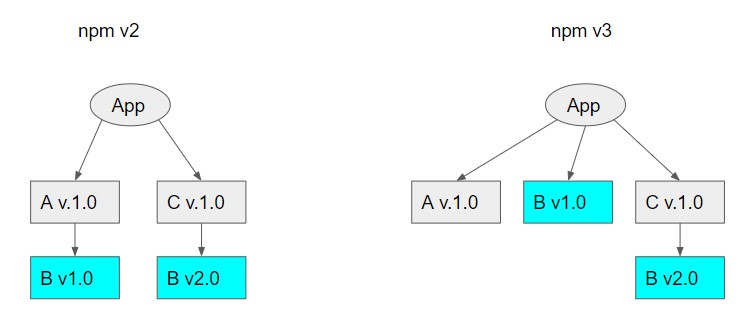
\includegraphics[width=.8\textwidth]{book/chapter-promisesandperils/pics/nestedv2.jpg}
	\caption{Difference between flat and nested dependencies}
	\label{fig:nest}
\end{figure}

\smallskip\noindent\textbf{Peril 5.}\textit{
Developers might declare a dependency to other parts of a software package ecosystem but not use it, e.g., because they failed to update its removal.
}\\

It is common for developers to declare dependencies on other parts of the software package ecosystem but not always use them. This can happen for various reasons, such as forgetting to remove the dependency after it is no longer needed. This can pose a challenge for researchers who are trying to extract dependencies from package managers, like those in configuration files, as there may be inconsistencies between the listed dependencies and what is actually being compiled and used by the code. This can lead to a biased understanding of the software package ecosystem and the relationships between software components.

To address this issue, there have been numerous efforts to track the actual library dependencies compiled and executed in software systems. These efforts aim to provide a more accurate understanding of the dependencies and the relationships between software components. For example, research has been conducted on the use of dynamic analysis to track compiled dependencies in real time and on the development of tools to automatically detect and track executed dependencies \cite{Zapata:ICSME2018, Ponta2018,Chinthanet:ASE2020}.

\subsection{Defining Boundaries and Completeness}

\smallskip\noindent\textbf{Promise 3.}\textit{
Researchers can use the boundaries of software package ecosystems to study communities of developers, e.g., developers contributing to and/or benefiting from the npm ecosystem.
}\\

Following Promise 2, the emergence of package managers has also led to studies that approximate software communities.
Using the libraries.io dataset, researchers were able to study projects that host libraries that use package managers.
Researchers have used this dataset to compare different library ecosystems \cite{kikas.2017,decan:emse:2019,CogoDown2019}.


\smallskip\noindent\textbf{Peril 6.}\textit{
Package managers do not always represent software package ecosystems, their communities, or their sub-communities, e.g., in cases where multiple package managers exist.
}\\

Package managers are a fundamental aspect of software package ecosystems, but do not always fully represent the complex relationships and interactions that occur within a community of developers and users, as shown in Table~\ref{tab:PM_features}. In some cases, multiple package managers exist for the same programming language, creating a complex landscape of software libraries and dependencies that are not always easily understood. For instance, Bower and Meteor manage npm libraries, which can lead to confusion and overlap in the management of dependencies.

Similarly, Java, Scala, Android, and other Java-based open source communities all use the Maven package manager, but each of these communities has its own unique set of libraries, dependencies, and development practises. Researchers should be aware of the limitations of package managers when studying software package ecosystems, and consider the broader context and relationships that exist within these communities. 

\smallskip\noindent\textbf{Peril 7.}\textit{
Lack of activity in parts of a software package ecosystem does not necessarily indicate project failure, e.g., when highly depended-upon libraries are feature-complete.
}\\

It is important to note that lack of activity in a part of a software package ecosystem does not always mean project failure \cite{coelho2017modern}. In some cases, highly relied-upon libraries that have reached feature-completeness may see little activity, but continue to be used by the software community. 

However, it is still important to consider the long-term sustainability of these libraries, especially given the rate at which technology and software development practises change. This has become a topic of interest in recent years, and researchers have explored best practises for sustaining open source projects and ensuring their continued success \cite{Ait2022,valiev2018ecosystem}. Understanding the factors that contribute to project sustainability is important to ensure the longevity and continued growth of software package ecosystems.

\smallskip\noindent\textbf{Peril 8.}\textit{
Sampling from a software package ecosystem is challenging since sub-setting might alter the dependency network, e.g., by breaking dependency chains.
}\\

Sampling from a package ecosystem is not straightforward, as the sample composition can be significantly affected due to missing dependency links between libraries. For instance, a subset of the ecosystem might alter the dependencies between libraries, leading to the breakdown of the dependency chains. This could lead to an incomplete picture of the software package ecosystem, leading to incorrect conclusions from a study. To minimise this risk, researchers should carefully consider the boundaries of their study and choose the appropriate sampling method based on the research questions and goals. For example, researchers could focus on popular, highly dependent, or risk-vulnerable aspects of the ecosystem as a starting point. 
For some ecosystems, the number of downloads, GitHub stars, and watchers are other aspects for the researcher to utilise.


\smallskip\noindent\textbf{Peril 9.}\textit{
Sampling from a software package ecosystem is challenging since the dependency network changes over time, e.g., when dependencies are added, removed, upgraded, or downgraded.
}\\

The dynamic nature of package ecosystems and the constant changes to their dependencies can impact the generalisability of the results. Therefore, it is important to also consider the time granularity of the analysis. For example, if the goal is to understand the evolution of dependencies over time, a finer time granularity may be necessary to capture the smaller changes and trends. However, if the goal is to understand the overall structure and relationships within the ecosystem, a coarser time granularity may be sufficient. Based on recent studies \cite{wattanakriengkrai2022giving,valiev2018ecosystem,Mirsaeedi:icse2020, Brindescu:emse2020, Nassif:icsme2017}, a three-month window seems appropriate for some studies.
Another level of granularity to consider is the size of the component. For instance, there are cases where a single package may contain more than one repository, especially for large library frameworks. 
The granularity also depends on the nature of the ecosystem itself. For instance, researchers should understand whether the ecosystem comprises library packages (e.g., PyPI), plugins (e.g., Eclipse), or is a library distribution (e.g., Android).



\subsection{Analysing and Visualising the Data}

\textbf{Peril 10.}\textit{
Analysing and visualising entire software package ecosystems is challenging due to their size, e.g., in terms of nodes and edges in the network.
}\\

The size of software package ecosystems implies large data sets, which can be overwhelming for tools and algorithms to analyse and display. Therefore, it may be necessary to make choices about the granularity of the data included in the analysis and visualisation. Another alternative is to focus on the most critical parts of the software package ecosystem, such as the high-level structure, highly dependent packages, or parts of the system that pose a risk to security and reliability. 
The key is to strike a balance between detail and simplicity, providing a meaningful representation of the ecosystem while being able to handle the complexity of its size.


\section{Application: When to Apply Which Peril}
\label{PPM:sec:application}

We include a disclaimer stating that not all perils are applicable to every mining situation. To demonstrate the practical application of our perils and their mitigation, we present two case studies that involve mining the software package ecosystem. Each case study has a distinct research objective and focusses on a specific dataset to be mined.

\subsection{Two Case Studies}
Table \ref{tab:cases} presents the two case studies we have selected for this analysis.
The \textit{first case} involves mining for contributions congruent to dependency updates \cite{wattanakriengkrai2022giving}. 
In this work, the authors mine GitHub repositories for Pull Requests and Issues that were submitted and merged congruent to dependency updates within the npm ecosystem. 
The \textit{second case} involves mining communication data for the Eclipse ecosystem \cite{Nugroho2021}. Although the second case does not mine for dependency relations (i.e., use relations),  we show that these perils still apply when mining for other relationships in an ecosystem.
Moreover, the second case studies the Eclipse ecosystem, which is a different dataset compared to the more popular GitHub dataset.

\subsection{Applying Perils and their Mitigation Strategies}
Table \ref{tab:perilsapp} provides a summary of the perils that can be applied to each of the case studies. We will now go into the details of mitigation strategies based on these perils. 
For better organisation and understanding, we have grouped the perils according to the four logical processes for mining.

\smallskip\noindent\textbf{Information to Mine}. 
The first set of mitigation strategies, which addresses perils 1-3, focusses on planning which information to mine. There are two primary strategies that researchers can employ:


\begin{enumerate}
    \item Researchers should use research tools and techniques to remove noise and other biases in the dataset, such as bot detection and the handling of multiple identities. This strategy was implemented in both case studies, as contributions and discussions often have the potential to involve bots or developers with multiple identities.
\item Depending on the research goals, researchers should recognise that not all contributions are equal and filter the dataset accordingly.
\end{enumerate}

We applied these two strategies to both cases. In the first case, the goal was to capture all congruent contributions, so we filtered out contributions made to libraries without dependencies. Since all npm packages are listed in the registry, Peril 3 (private activities) did not apply.
In the second case, we addressed Peril 1 by conducting a qualitative analysis to ensure that the member identities were not duplicated, as Eclipse developers were known to change identities. To mitigate Peril 2, we removed bot responses. For the second case, since all forum data is made public, Peril 3 did not apply.


\begin{table}
\centering
\caption{Description of the research objectives and datasets for the case studies}
 \label{tab:cases}
\begin{tabular}{lp{5cm}r} 
\toprule
\textbf{Case Study} & \textbf{Research Objective}                                                          & \textbf{Datasets}           \\
\midrule
Wattanakriengkrai \etal \cite{wattanakriengkrai2022giving}             & Explore code contributions between library and client (i.e, use-relations)  & libraries.io\\
& &  GitHub API \\
Nugroho \etal \cite{Nugroho2021}                & Explore discussion contributions between contributors (i.e., contributions) & Eclipse API                \\
\bottomrule
\end{tabular}
\end{table}

\begin{table}
\centering
\caption{Application of each peril to the case studies}
 \label{tab:perilsapp}
\begin{tabular}{rp{8cm}ccc} 
\toprule                   
& \textbf{Perils}       & case 1      & case 2                 \\
                                                                               & & npm  & Eclipse   \\
\midrule
\textbf{P1} &Developers might use different identifiers when contributing to different parts of a software package ecosystem, e.g., when contributing to different libraries.                             &    \CheckedBox         &          \CheckedBox           \\ 
%\hline
\textbf{P2} & Developers' contributions to software package ecosystems might be interspersed with bot contributions, e.g., automated dependency updates.                                                      &      \CheckedBox               &      \CheckedBox               \\ 
%\hline
\textbf{P3} & Not all developer activities in software package ecosystems are accessible to the public, e.g., library use in proprietary settings.                                                         &         -           &      \CheckedBox               \\ 
%\hline
\textbf{P4} & Different software package ecosystems define the concept of \`{}\`{}dependency'' differently, e.g., by allowing or not allowing different versions of a library on the same dependency tree. &         \CheckedBox       &     -                            \\ 
%\hline
\textbf{P5} & Developers might declare a dependency to other parts of a software package ecosystem but not use it, e.g., because they failed to update its removal.                                        &     -           &  -    \\
%\hline
\textbf{P6} &Package managers do not always represent software package ecosystems, their communities, or their sub-communities, e.g., in cases where multiple package managers exist.                     &     -                   &  -                  \\
%\hline
\textbf{P7} & Lack of activity in parts of a software package ecosystem does not necessarily indicate project failure, e.g., when highly depended-upon libraries are feature-complete.                     &       \CheckedBox         &  -                           \\
%\hline
\textbf{P8} &Sampling from a software package ecosystem is challenging since sub-setting might alter the dependency network, e.g., by breaking dependency chains.                                         &        \CheckedBox        &     \CheckedBox                                \\
%\hline
\textbf{P9} &Sampling from a software package ecosystem is challenging since the dependency network changes over time, e.g., when dependencies are added, removed, upgraded, or downgraded.               &       \CheckedBox         &     -                          \\
%\hline
\textbf{P10} &Analysing and visualising entire software package ecosystems is challenging due to their size, e.g., in terms of nodes and edges in the network.                                  &        \CheckedBox      &      \CheckedBox               \\
\bottomrule
\end{tabular}
\end{table}

\smallskip\noindent\textbf{Defining Dependencies}. 
The second set of perils (Perils 4-5) is related to dependency relationships between software units, and only the first case study is applicable. To address these perils, researchers should adopt the following strategy:

\begin{enumerate}
    \item Researchers should not rely solely on listed dependencies in configuration files (e.g., pom.xml, package.json, etc.) as a measure of dependency between two components. Instead, code-centric approaches should be used to validate which libraries are actually depended upon.
\end{enumerate}

For example, in the first case, in addition to mining the configuration information, the authors also analysed the similarity of the source code contributions to address Peril 4. Regarding Peril 5, since the study's objective was to investigate changes to the configuration files, the risk of the update not being executed was deemed less important.
It is important to note that the second case study did not include dependency analysis and, therefore, these perils did not apply.

\begin{figure*}[]
    \centering
    \begin{subfigure}{0.9\linewidth}
         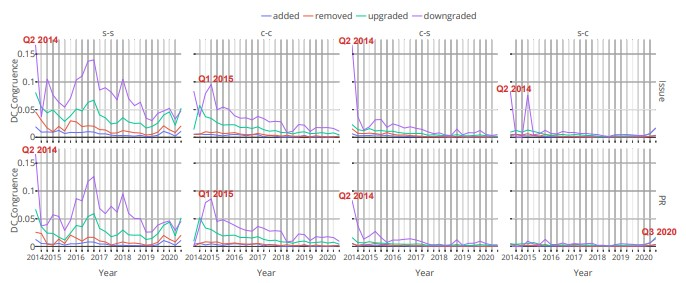
\includegraphics[width=1.1\textwidth]{book/chapter-promisesandperils/pics/congruentViz.jpg}
         \caption{Visualization of a Time analysis for 107,242 libraries.}
     \end{subfigure}
     \begin{subfigure}{0.9\linewidth}
         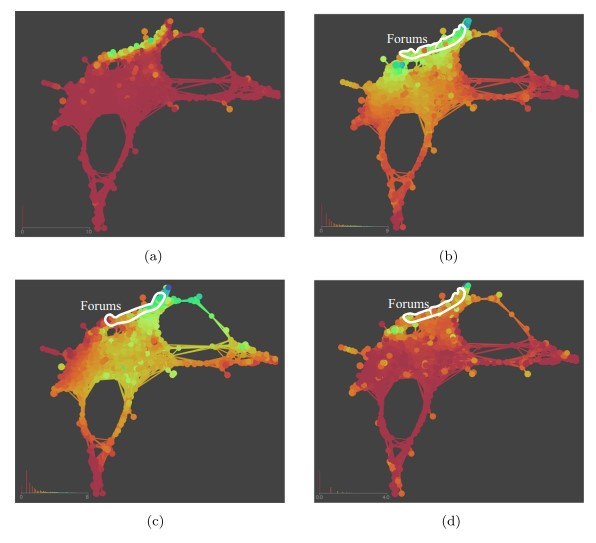
\includegraphics[width=1\textwidth]{book/chapter-promisesandperils/pics/eclipseViz.jpg}
         \caption{A Visual Topology map for 832,058 threads}
     \end{subfigure}
    \caption{Visualisation examples for the two case studies}
    \label{fig:visCase}
\end{figure*}

\smallskip\noindent\textbf{Defining Boundaries}.
The third set of perils (Perils 6-9) is related to the definition of boundaries and completeness and is relevant for both case studies. To mitigate these perils, we recommend the following strategies:

\begin{enumerate}
    \item Researchers should recognise that a dormant project does not necessarily mean that it is inactive. Instead, studies can use alternative heuristics, such as the number of dependents and dependencies, as better indicators of a project's importance in the ecosystem.
    \item Researchers should not rely solely on the programming language to define sub-communities. Using a common package manager for the programming language is a more effective rule of thumb for distinguishing boundaries.
    \item Researchers should avoid random sampling. Instead, sampling should be tailored to the research goals by considering factors such as an appropriate time window or focussing on specific attributes of components (e.g., most dependents, most popular, most contributors).
\end{enumerate}


Peril 6 did not apply to any of the case studies. 
Particularly for the first case, since the goal was to explore the npm package ecosystem, we assumed that the boundaries were clearly defined by the npm registry. 
Similarly, the second case study used the generic Eclipse platform as the boundary. 
Peril 7 was applied to the npm study, while Peril 8 was applied to both case studies. 
As a result, the two cases conducted a qualitative analysis of the dataset to gain deeper insights.
In the first case study, a three-month time window was created to capture dependencies. 
For the second case study, forum contributors were sampled into three groups (i.e., junior, member, or senior) according to the sliding window of their contributions. 

\smallskip\noindent\textbf{Visualisation}.
The final peril (Peril 10) relates to visualisation, which can be challenging due to the vast size and complexity of software ecosystems. As it is not feasible to visualise every aspect of an ecosystem simultaneously, a focused approach is necessary. A mitigation strategy is to select specific attributes of the ecosystem (e.g., the most dependent, most popular, and most contributions) that align with the research needs and objectives. 

Figure \ref{fig:visCase} shows two cases where visualizations are employed to gain insights, especially for large datasets.
In the first figure (a), we visualize the distributions of the data set and applied the appropriate statistical tests, along with the effect size, to test our hypotheses and answer research questions. 
In the second example (b), although not directly related to package ecosystems, the authors utilized a topological visualization \cite{Lum2013ExtractingIF} to gain insights on the over 800,000 forum threads of discussions. 



\section{Chapter Summary}
In this chapter, we explore the various aspects of mining information from the software package ecosystem, presenting three promises and ten perils that researchers should be aware of when undertaking such tasks. The chapter is structured around four key processes for mining: 1) Planning what Information to Mine, 2) Defining Components and their Dependencies, 3) Defining Boundaries and Completeness, and 4) Analysing and Visualising the Data. To help new and experienced researchers navigate these challenges, we introduced the SUG model, which can serve as a valuable tool to minimise threats to validity. Although some perils may be more relevant to specific research objectives, our aim is to equip researchers with the knowledge and resources needed to confidently gather and integrate software package ecosystem data into their work.
 %Managing modeling ecosystems by means of machine learning techniques
% %Semantic labeling three-letter-code: MDE (e.g. \chapter{MDE})

% 
\title{Promises and Perils of Mining \\ Software Package Ecosystem Data}
\author{Raula Gaikovina Kula \and Katsuro Inoue \and Christoph Treude}
\institute{Raula Gaikovina Kula \at Nara Institute of Science and Technology, Japan, \email{raula-k@naist.jp}
\and Katsuro Inoue \at Nanzan University, Japan \email{ inoue599@nanzan-u.ac.jp}
\and  Christoph Treude \at The University of Melbourne, Australia \email{christoph.treude@unimelb.edu.au}}

\maketitle
\label{PPM:ch}
\abstract*{The use of third-party packages is becoming increasingly popular and has led to the emergence of large software package ecosystems with a maze of inter-dependencies. Since the reliance on these ecosystems enables developers to reduce development effort and increase productivity, it has attracted the interest of researchers: understanding the infrastructure and dynamics of package ecosystems has given rise to approaches for better code reuse, automated updates, and the avoidance of vulnerabilities, to name a few examples. But the reality of these ecosystems also poses challenges to software engineering researchers, such as: How do we obtain the complete network of dependencies along with the corresponding versioning information? What are the boundaries of these package ecosystem? How do we consistently detect dependencies that are declared but not used? How do we consistently identify developers within a package ecosystem? How much of the ecosystem do we need to understand to analyse a single component? How well do our approaches generalise across different programming languages and package ecosystems? In this chapter, we review promises and perils of mining the rich data related to software package ecosystems available to software engineering researchers.}

\abstract{The use of third-party packages is becoming increasingly popular and has led to the emergence of large software package ecosystems with a maze of inter-dependencies. Since the reliance on these ecosystems enables developers to reduce development effort and increase productivity, it has attracted the interest of researchers: understanding the infrastructure and dynamics of package ecosystems has given rise to approaches for better code reuse, automated updates, and the avoidance of vulnerabilities, to name a few examples. But the reality of these ecosystems also poses challenges to software engineering researchers, such as: How do we obtain the complete network of dependencies along with the corresponding versioning information? What are the boundaries of these package ecosystems? How do we consistently detect dependencies that are declared but not used? How do we consistently identify developers within a package ecosystem? How much of the ecosystem do we need to understand to analyse a single component? How well do our approaches generalise across different programming languages and package ecosystems? In this chapter, we review promises and perils of mining the rich data related to software package ecosystems available to software engineering researchers.}

%%%%%%%%%%%%%%%%%%%%%%%%%%%%%%%%%%%%%%%%%%%%%%%%%%%%%%%%%%%%%%%%%%

\section{Introduction}
\label{PPM:sec:definition}

Third-party libraries are a great way for developers to incorporate code without having to write their own for every functionality required. By using these libraries, developers can save time and energy while still getting the functions they need.
Using third-party libraries is becoming increasingly popular and has led to the emergence of large software package ecosystems such as npm. While these ecosystems offer many benefits, they also come with risks, such as software vulnerability attacks \cite{Chinthanet:ASE2020}.

Large software package ecosystems are a treasure trove for researchers who can investigate a wide range of questions. For example, by studying activity in large ecosystems, researchers can identify which libraries are the most popular and learn what characteristics make them successful \cite{kikas.2017,decan:emse:2019}.
Additionally, research on large ecosystems can help developers understand how to protect their code from malicious actors who may attempt to exploit vulnerabilities or insert malware into popular libraries.
Studying large software package ecosystems can help us better understand the dynamics of open source development in general. Open source development is a complex process that involves many different stakeholders working together (or sometimes competing) to create valuable code that anyone can use or improve upon. By understanding how these interactions play out in different types of ecosystem structures -- including those with many small projects versus few very large ones -- we can develop insights that might be applicable more broadly across other types of collaborative systems.

In this chapter, we identify and discuss promises and perils during the mining process, ranging from planning what information to mine from the ecosystem to analysing and visualising the mined data. 
Therefore, the chapter is broken down into these logical processes of mining ecosystem data: 1) Planning what Information to Mine, 2) Defining Components and their Dependencies, 3) Defining Boundaries and Completeness, and 4) Analysing and Visualising the Data.

This chapter is intended for researchers and practitioners who are interested in exploring and exploiting software package ecosystem information from a diverse range of sources that are publicly available. 
We also highlight the pitfalls to consider during the mining process, particularly when these pitfalls could lead to a misinterpretation of the analysis and results. 
The chapter is written in a manner that encourages newcomers who have little or no experience or who are interested in utilising ecosystem data across different disciplines outside of software engineering.
Our goal is to get new researchers quickly accustomed to gathering ecosystem information for their research.


\section{A Component-based Software Ecosystem}

Defined as a component-based software ecosystem, we suggest using the term `software package ecosystem' as a suitable term for the symbiotic relationships among third-party library components (as software projects or repositories), as these libraries and their dependent clients coexist on the same technological platform, therefore sharing the same environment and other internal and external factors (e.g., security threats, sharing contributions, etc.).
Please refer to the Introduction chapter for an in-depth definition of the different types of software ecosystems.
We present our interpretation of the software package ecosystem in Kula et al.~\cite{KulaSANER18}, where we formally define a package ecosystem using a Software Universe Graph (SUG).
This is modelled as a structured abstraction of the evolution of software systems and their library dependencies over time.

%%%%%%%%%%%%%%%%%%%%%%%%%%%%%%%%%%%%%%%%%%
\begin{figure*}
	\centering
	\includegraphics[width=.7\textwidth]{book/chapter-promisesandperils/pics/UniversalExample.jpg}
	\caption{Conceptual example of the Software Universe Graph, depicting the use and update relationships between different software units.}
	\label{fig:SUG}
\end{figure*}
%%%%%%%%%%%%%%%%%%%%%%%%%%%%%%%%%%%%%%%%%%%%%


\paragraph{\textbf{Component-based Representation as a Software Universe Graph}}
\label{PPM:sec:SUG}

First introduced by Kula et al.~\cite{KulaSANER18}, the \textit{Software Universe Graph} (SUG) is a structural abstraction of the software ecosystem of third-party libraries.
Figure \ref{fig:SUG} provides an illustration of the different relationships within the graph.
Let $G= (N,E)$ represent a graph $G$. $N$ is a set of nodes, each node representing a software unit. 
We define a software unit as a version instance of any software program. 

The authors then present the \textit{use} and \textit{update} relationships that exist in the ecosystem.
Hence, the edges $E$ are composed of $E_{use}$ and $E_{update}$. $E_{use}$ is a set of \textit{use-relations} and $E_{update}$ is a set of \textit{update-relations}.

\begin{definition}
An edge $u \rightarrow v \in E_{use}$ means that $u$ uses $v$. The defined functions of $E_{use}$ are:

\begin{equation}
\small
\small \use(u)\equiv \{v|u \rightarrow v\}
\normalsize
\end{equation}
\begin{equation}
\small
\small \useBy(u)\equiv \{v|v \rightarrow u\}
\normalsize
\end{equation}
\end{definition}

Use-relations can be extracted from either the source code or configuration files. 
As shown in Figure \ref{fig:SUG}, node $a1$ uses node $x1$. 
In addition, node $x1$ is used by nodes $a1$, $q1$, and $q2$. Parallel edges for node pairs are not allowed.

\begin{definition}
We represent an update relation from node $a$ to $b$ using $ a \Rightarrow b $, which means that the newer update $b$ was released from node $a$ and is defined as:
\begin{equation}
\small a \Rightarrow b \in E_{update}
\end{equation}
\end{definition}

Update relations refer to when a successive release of a software unit is made available. Figure \ref{fig:SUG} shows that node $q1$ is first updated to node $q2$. Later, node $q2$ is updated to the latest node $q3$. Hence, $q1 \Rightarrow q2 \Rightarrow q3$.
Note that an update should not be confused with forking. 
We distinguish a fork as a separate software unit. 
Each node in the SUG should be denoted by three attributes: \texttt{<name,release,time>}.  
For a node $u$, we define:

\begin{itemize}
	\item \textbf{u.name} Name is the string representation identifier of a software unit.
	We introduce the name axiom: For nodes $u$ and $v$, if $u \Rightarrow v$, then $u.name = v.name$ holds.
	
	\item \textbf{u.release}. Release refers to the specific assigned change reference for a software unit. For nodes $u$ and $v$, if $u \Rightarrow v$
	then $v$ is the immediate successor of $u$. Note that the versioning pattern may vary from project to project. 
	\item \textbf{u.time}. Time refers to the time stamp at which node $u$ was released. For nodes $u$ and $v$ of $u \Rightarrow v$, $u.time < v.time$.
\end{itemize}

\begin{figure}
	\centering
	\includegraphics[width=.8\textwidth]{book/chapter-promisesandperils/pics/TemporalSUG.jpg}
	\caption{Temporal property of the SUG}
	\label{fig:SUGTemp}
\end{figure}

\begin{definition}
    
	The SUG has temporal properties.
This describes the simultaneity or ordering in reference to time. Let SUG $G = (N, E) $ be at time $t$. At time $t^{\prime} > t$, we observe an extension of $G$, such that:

\begin{equation}
\small G^{\prime} = (N \cup \Delta N, E \cup \Delta E)
\end{equation}
where $\Delta E \cap (N \times N) = \emptyset$
\end{definition}

Figure \ref{fig:SUGTemp} illustrates the temporal properties of the SUG. 
Here, it is observed that $G'$ is composed of $G$ augmented with newly added node $a3$ and its corresponding $a3 \rightarrow x2$ and $a2 \Rightarrow a3$ relations.
A SUG grows monotonically over time with only additions.
Here, we consider that modification or deletion changes on the SUG do not occur. 

\begin{definition}
    A timed SUG specifies the state of the SUG at any point in time.
So for an SUG $G=(N,E)$, we represent a timed SUG $G_{t}$ at time $t$ as a sub-graph of $G$. Formally,
\begin{equation}
\small G_t\equiv(N_{t}, E_{t})
\end{equation}
where $N_{t} = \{u|u \in N, u.time \leq t \}$ and $E_t = \{ e | e \in E \wedge e \in  N_t \}$
\end{definition}
	


\section{Data Sources}
Researchers can use various datasets to model the ecosystem using the SUG model of usage and update relationships.
The most obvious data source that has revolutionised data mining in the software engineering domain is the GitHub platform. 
Established in 2008, and then purchased by Microsoft in 2020, GitHub is home to various popular Open Source Software. 
GitHub is built on the git version control system and is useful for storing all changes made to a repository. 
In the case of the SUG, a GitHub repository can represent one software unit, whose depend relations can be extracted via a configuration file (such as the package.json file for JavaScript projects).
The repository should also contain the release information that holds the update relations.
Due to its large size, researchers and the GitHub team have made available datasets for researchers to mine, for example through the GitHub API/Graph QL.\footnote{\url{https://docs.github.com/en/graphql}} This is the backend Application Programming Interface (API) that can be used to query large amounts of data on GitHub. Most researchers use the API to download and mine information from the GitHub platform. 
It is important to note that while GitHub introduced a new feature of Dependency Graphs to map the depend relationship,\footnote{\url{https://docs.github.com/en/code-security/supply-chain-security/understanding-your-software-supply-chain/about-the-dependency-graph}} most older projects do not have this feature.
In this case, the researcher would need to manually extract and query the configuration files for dependency information. 

We refer to the first chapter for additional information on data sources for mining software ecosystems. 

\section{Promises and Perils}
\label{PPM:sec:promisesperils}

Using the SUG model of depend and use relations and the available datasets, we can now present our promises and perils of mining ecosystem information.

\subsection{Planning What Information to Mine}

\textbf{Promise 1.}\textit{
Researchers can access and link heterogeneous data related to software package ecosystems, e.g., package registries and bug trackers.}\\

When planning what information to mine from the ecosystem, researchers do not need to limit themselves to the usage and update relationship information.
Platforms that host software repositories include other software management systems such as bug trackers.
For example, GitHub allows researchers to manage GitHub Pull Requests, Issues, and Discussions not only for one project, but for multiple projects.
GitHub provides three management systems that are related to a software repository:

\begin{itemize}
    \item \textit{GitHub Discussions}\footnote{\url{https://docs.github.com/en/discussions}} - The GitHub Discussions forum is a collaborative communication forum for the community around an open source or internal project. Community members can ask and answer questions, share updates, have open-ended conversations, and follow along on decisions affecting the community's way of working.
    \item \textit{GitHub Pull Requests}\footnote{\url{https://docs.github.com/en/pull-requests}} - Pull Requests allow other developers from an ecosystem to make a contribution to a software repository. Pull requests also allow maintainers to discuss and review potential changes with collaborators and add follow-up commits before changes are merged into the software.
    \item \textit{GitHub Issues}\footnote{\url{https://docs.github.com/en/issues}} - Issues are used to track ideas, feedback, tasks, or bugs for work on GitHub.
\end{itemize}

These three systems are examples of how developers contribute to both their own and other projects. 
Hence, to incorporate this information, we can extend the SUG model, creating a model that includes a contribution relationship \cite{wattanakriengkrai2022giving}.

% Note that other platforms may also have management systems, like GitLab, BitBucket and Eclipse.

\begin{definition}
	A Dependency-Contribution graph incorporates contributions by developers whose libraries are involved in dependency relationships. 
\end{definition}

In this work \cite{wattanakriengkrai2022giving}, the authors explore the congruence between dependency updates and developer contributions, based on the original concept of social-technical congruence \cite{stcCataldo2008} where developers contribution patterns are congruent with their coordination needs. Hence, the goal is to identify contributions that are congruent to dependency updates.
As shown in Figure \ref{fig:lib} the authors extend from the typical SUG graph model where $lib_i$ depends (use) on  $lib_k$ and  $lib_j$, while  $lib_j$ also depends on $lib_k$, to the example shown in Figure \ref{fig:dc-graph}.
Different to the SUG, the graph captures developers and their contributions (i.e., the square as $dev_x$ and $dev_y$ represent two different developers making a contribution).
Here contributions are defined as $c$ (Pull Request or Issue) that were submitted to both a library and the client that depends on that library.
Hence, the graph can show contributions that are congruent to dependency changes for a software unit. 

\begin{figure}[t]
     \centering
     \begin{tikzpicture}[
         roundnode/.style={circle, fill=black, minimum size=5mm},
        squarenode/.style={fill=black, text=red, minimum size=5mm},
     ]
    \begin{scope}
         \node[roundnode, label=above:$lib_i$] (s2_proji) at (3, 2.5) {};
        \node[roundnode, label=below:$lib_j$] (s2_projj) at (4,0) {};
         \node[roundnode, label=below:$lib_k$] (s2_projk) at (2,0) {};
     \end{scope}

     \begin{scope} [every edge/.style={draw=gray, very thick}]
         \path [->] (s2_proji) edge (s2_projj);
         \path [->] (s2_proji) edge (s2_projk);
         \path [->] (s2_projj) edge (s2_projk);
     \end{scope}
     \end{tikzpicture}
    
     \caption{Example dependency graph for a given time period}
     \label{fig:lib}
     \vspace{2ex}
 \end{figure}
\begin{figure}[t]
    \centering

    \begin{tikzpicture}[
        roundnode/.style={circle, fill=black, minimum size=5mm},
        squarenode/.style={fill=black, text=red, minimum size=5mm},
    ]
    \begin{scope}
        
        \node[roundnode, label=right:$lib_i$] (s2_proji) at (4, 1.5) {};
        \node[roundnode, label=below:$lib_j$] (s2_projj) at (5,0) {};
        \node[roundnode, label=below:$lib_k$] (s2_projk) at (3,0) {};
        
        \node[squarenode, label=below:$dev_x$] (s3_devx) at (2, 3.5) {};
        
        \node[squarenode, label=below:$dev_y$] (s3_devy) at (6, 3.5) {};
        
    \end{scope}

    \begin{scope} [every edge/.style={draw=gray, very thick}]
        \path [->] (s2_proji)  edge  (s2_projj);
        \path [->] (s2_proji) edge (s2_projk);
        \path [->] (s2_projj) edge (s2_projk);
        
    \end{scope}
    \begin{scope} [every edge/.style={draw=gray, thick, double distance=2pt}]
        \path [->] (6, 2.8) edge node[left = 2mm] {$contribute$} (s2_proji);
        \path [->] (6, 2.8) edge[bend left=15] node[right = 1mm] {$contribute$} (s2_projj);
        \path [->] (2, 2.8) edge node[right = 2mm] {$$} (s2_proji);
        \path [->] (2, 2.8) edge[bend right=15] node[left = 1mm] {$contribute$} (s2_projk);
    \end{scope}
    \end{tikzpicture}
\end{figure}
\begin{figure}[t]
    \centering
    \begin{tikzpicture}[
        roundnode/.style={circle, fill=black, minimum size=5mm},
        squarenode/.style={fill=black, text=red, minimum size=5mm},
    ]
    \end{tikzpicture}
\caption{Example Dependency-Contribution graph showing relationships between contributions and dependencies}
 \label{fig:dc-graph}
\end{figure}

This is just one example of the type of research that is enabled by access to heterogeneous data related to software package ecosystems.

\smallskip\noindent\textbf{Peril 1.}\textit{
 Developers might use different identifiers when contributing to different parts of a software package ecosystem, e.g., when contributing to different libraries.}\\
 
When modelling using such graphs, there is a threat that contributors may use multiple identifiers (i.e., $c_x$ and $c_y$ are the same contributor).
This is a well-known research problem, and there has been work to merge these accounts, such as \cite{wiese2016mailing}.
GitHub has introduced mechanisms such as two-factor authentication\footnote{\url{https://docs.github.com/en/authentication/securing-your-account-with-two-factor-authentication-2fa/configuring-two-factor-authentication}} to counteract the issue of multiple identifiers.
This is since developers might be less likely to switch accounts if it requires cumbersome authentication.


\smallskip\noindent\textbf{Peril 2.}\textit{
Developers' contributions to software package ecosystems might be interspersed with bot contributions, e.g., automated dependency updates.}\\

The rise of automation and artificial intelligence has led to much work on the integration of automated scheduling (i.e., bots) into software development workflows \cite{Storey2016, Farooq2016, Wessel2018, Erlenhov2019, bot_modify_wf} to name a few. These bots are designed to perform specific tasks within a software package ecosystem. For example, a bot may be programmed to automatically update dependencies, test code changes, or deploy software to production. As an example, the Google APIs repo-automation-bots project lists bots for automated labelling of issues and pull requests, automated approval of pull requests, and triggering releases.\footnote{\url{https://github.com/googleapis/repo-automation-bots}}
Bots perform common maintenance tasks in many software projects and are now commonplace \cite{Beschastnikh2017, Urli2018,BIMAN,bot_or_not}.
Especially with bots such as dependabot (automated pull requests to update configurations to reduce the risk of vulnerability threats),\footnote{\url{https://github.com/dependabot}} more and more automation has caused a lot of noise in the contributions between projects.
There are also bots for communication and documentation \cite{Urli2018, Lin2016, Lebeuf2017a}.

To be able to draw accurate conclusions about what humans are doing in software package ecosystems, researchers should consider distinguishing between bot and human contributions.
It is also important to differentiate this from other contributions \cite{maeprasart2022understanding}.
The research community has responded well, with a wide range of techniques and tools to mitigate this peril \cite{Bodegha2021, golzadeh2022accuracy}.

\smallskip\noindent\textbf{Peril 3.}\textit{
Not all developer activities in software package ecosystems are accessible to the public, e.g., library use in proprietary settings.
}\\

Not all developer activities in software package ecosystems are accessible to the public, e.g., when the boundary between open source and industry is blurred \cite{stol2014inner}, which presents a challenge for researchers who aim to study the development process. This is particularly true in proprietary settings where software development is performed behind closed doors or is open source for a limited time period, thus resulting in the artefacts not permanently being publicly available.
This can make it difficult to understand the broader ecosystem in which a software project is developed.
Proprietary settings may lead to non-standardisation in software development practises. Different software projects may use different management systems and tools, making it difficult to accurately compare and analyse software development activities across various projects. For example, some projects may use communication, documentation, and other management tools not captured on the same platform \cite{montgomery2022alternative}. For example, some projects might use Bugzilla instead of issues and pull requests for their bug and code review systems, while others may use Discord, Slack channels, or email threads for their communication needs.

This lack of standardisation in software development practises presents a challenge for researchers who study the software package ecosystem and understand the development process. To address this issue, researchers should strive to collect data from a diverse set of projects to gain a comprehensive understanding of the software package ecosystem. In addition, researchers may need to adjust their methodologies or data collection techniques to accommodate the different tools and practises used by different software projects.

\subsection{Defining Components and their Dependencies}

\smallskip\noindent\textbf{Promise 2.}\textit{
Researchers can access a software package ecosystem's dependency network through package managers and registries, e.g., npm lists the dependencies and dependents for over a million libraries.}\\


With the rise of curated datasets like libraries.io, researchers can now recover and model dependency relations between software units using pre-extracted datasets.
Table \ref{tab:PM_features} shows examples of popular package managers mined from the libraries.io dataset in 2020. 

\begin{table*}[]
\caption{Summary of 13 package managers from libraries.io as ranked by TIOBE in 2020}
 \label{tab:PM_features}
 \centering
\begin{tabular}{@{}llrlll@{}}
\toprule
\begin{tabular}[c]{@{}l@{}}Package \\ Ecosystem\end{tabular} & \begin{tabular}[c]{@{}l@{}}Programming \\ Language\end{tabular} &  \begin{tabular}[c]{@{}l@{}}Tiobe \\ Rank\end{tabular} & Environment & \begin{tabular}[c]{@{}l@{}}Dependency \\ Tree\end{tabular} & \begin{tabular}[c]{@{}l@{}}Package   \\Archive link\end{tabular}\\ \midrule
PyPI & Python & 2 & Python & Flat & pypi.org  \\
Maven & Java & 3 & JVM & Flat & Maven.org  \\
Bower & JavaScript & 7 & Node.js & Flat & bower.io  \\
Meteor & JavaScript & 7 & Node.js & Nested & atmospherejs.com \\
npm & JavaScript & 7 & Node.js & Nested (v2) & npmjs.com  \\
Packagist & PHP & 8 & PHP & Flat & packagist.org \\
Puppet & Ruby & 13 & Ruby MRI & Flat & forge.puppet.com  \\
RubyGems & Ruby & 13 & Ruby MRI & Flat & rubygems.org  \\
CRAN & R & 14 & RStudio & Flat & cran.r-project.org  \\
CPAN & Perl & 15 & Perl & Flat & metacpan.org  \\
GO & Golang & 20 & Go & Flat & pkg.go.dev  \\
NuGet & C\#, VB & 5, 6 & .NET & Flat & nuget.org \\
Anaconda & Python, R, C\# & 2, 14, 5 & Anaconda & Flat & anaconda.org  \\ \bottomrule
\end{tabular}
\end{table*}

\smallskip\noindent\textbf{Peril 4.}\textit{
Different software package ecosystems define the concept of ``dependency'' differently, e.g., by allowing or not allowing different versions of a library on the same dependency tree.
}\\

Different software package ecosystems have varying definitions of what constitutes a dependency. For example, some ecosystems may allow multiple versions of a library to exist on the same dependency tree, while others may restrict developers to a single version of a library \cite{Islam}. These restrictions are often based on the programming language being used, as different languages have different approaches to managing dependencies. It is important to consider the restrictions on dependency relationships when studying software package ecosystems, as they can have a major impact on the development process. For example, the ability to use multiple versions of a library on the same dependency tree can greatly simplify the process of updating dependencies and can make it easier to resolve conflicts between libraries.

One way to visualise the impact of these restrictions is to compare the difference between a nested dependency tree and a directed dependency tree, as shown in Figure \ref{fig:nest}.\footnote{Taken from \url{https://npm.github.io/how-npm-works-docs/npm3/how-npm3-works.html}} This distinction is important because it highlights the different ways that a software unit can depend on different versions of the same library.
In this example, npm v3 creates the dependency tree based on the installation order, therefore flattening unnecessary nested dependencies (i.e., B v1.0 in cyan). This reduces the complexity of a nested tree by resolving some of the transitive dependencies (nested dependencies).

\begin{figure}
	\centering
	\includegraphics[width=.8\textwidth]{book/chapter-promisesandperils/pics/nestedv2.jpg}
	\caption{Difference between flat and nested dependencies}
	\label{fig:nest}
\end{figure}

\smallskip\noindent\textbf{Peril 5.}\textit{
Developers might declare a dependency to other parts of a software package ecosystem but not use it, e.g., because they failed to update its removal.
}\\

It is common for developers to declare dependencies on other parts of the software package ecosystem but not always use them. This can happen for various reasons, such as forgetting to remove the dependency after it is no longer needed. This can pose a challenge for researchers who are trying to extract dependencies from package managers, like those in configuration files, as there may be inconsistencies between the listed dependencies and what is actually being compiled and used by the code. This can lead to a biased understanding of the software package ecosystem and the relationships between software components.

To address this issue, there have been numerous efforts to track the actual library dependencies compiled and executed in software systems. These efforts aim to provide a more accurate understanding of the dependencies and the relationships between software components. For example, research has been conducted on the use of dynamic analysis to track compiled dependencies in real time and on the development of tools to automatically detect and track executed dependencies \cite{Zapata:ICSME2018, Ponta2018,Chinthanet:ASE2020}.

\subsection{Defining Boundaries and Completeness}

\smallskip\noindent\textbf{Promise 3.}\textit{
Researchers can use the boundaries of software package ecosystems to study communities of developers, e.g., developers contributing to and/or benefiting from the npm ecosystem.
}\\

Following Promise 2, the emergence of package managers has also led to studies that approximate software communities.
Using the libraries.io dataset, researchers were able to study projects that host libraries that use package managers.
Researchers have used this dataset to compare different library ecosystems \cite{kikas.2017,decan:emse:2019,CogoDown2019}.


\smallskip\noindent\textbf{Peril 6.}\textit{
Package managers do not always represent software package ecosystems, their communities, or their sub-communities, e.g., in cases where multiple package managers exist.
}\\

Package managers are a fundamental aspect of software package ecosystems, but do not always fully represent the complex relationships and interactions that occur within a community of developers and users, as shown in Table~\ref{tab:PM_features}. In some cases, multiple package managers exist for the same programming language, creating a complex landscape of software libraries and dependencies that are not always easily understood. For instance, Bower and Meteor manage npm libraries, which can lead to confusion and overlap in the management of dependencies.

Similarly, Java, Scala, Android, and other Java-based open source communities all use the Maven package manager, but each of these communities has its own unique set of libraries, dependencies, and development practises. Researchers should be aware of the limitations of package managers when studying software package ecosystems, and consider the broader context and relationships that exist within these communities. 

\smallskip\noindent\textbf{Peril 7.}\textit{
Lack of activity in parts of a software package ecosystem does not necessarily indicate project failure, e.g., when highly depended-upon libraries are feature-complete.
}\\

It is important to note that lack of activity in a part of a software package ecosystem does not always mean project failure \cite{coelho2017modern}. In some cases, highly relied-upon libraries that have reached feature-completeness may see little activity, but continue to be used by the software community. 

However, it is still important to consider the long-term sustainability of these libraries, especially given the rate at which technology and software development practises change. This has become a topic of interest in recent years, and researchers have explored best practises for sustaining open source projects and ensuring their continued success \cite{Ait2022,valiev2018ecosystem}. Understanding the factors that contribute to project sustainability is important to ensure the longevity and continued growth of software package ecosystems.

\smallskip\noindent\textbf{Peril 8.}\textit{
Sampling from a software package ecosystem is challenging since sub-setting might alter the dependency network, e.g., by breaking dependency chains.
}\\

Sampling from a package ecosystem is not straightforward, as the sample composition can be significantly affected due to missing dependency links between libraries. For instance, a subset of the ecosystem might alter the dependencies between libraries, leading to the breakdown of the dependency chains. This could lead to an incomplete picture of the software package ecosystem, leading to incorrect conclusions from a study. To minimise this risk, researchers should carefully consider the boundaries of their study and choose the appropriate sampling method based on the research questions and goals. For example, researchers could focus on popular, highly dependent, or risk-vulnerable aspects of the ecosystem as a starting point. 
For some ecosystems, the number of downloads, GitHub stars, and watchers are other aspects for the researcher to utilise.


\smallskip\noindent\textbf{Peril 9.}\textit{
Sampling from a software package ecosystem is challenging since the dependency network changes over time, e.g., when dependencies are added, removed, upgraded, or downgraded.
}\\

The dynamic nature of package ecosystems and the constant changes to their dependencies can impact the generalisability of the results. Therefore, it is important to also consider the time granularity of the analysis. For example, if the goal is to understand the evolution of dependencies over time, a finer time granularity may be necessary to capture the smaller changes and trends. However, if the goal is to understand the overall structure and relationships within the ecosystem, a coarser time granularity may be sufficient. Based on recent studies \cite{wattanakriengkrai2022giving,valiev2018ecosystem,Mirsaeedi:icse2020, Brindescu:emse2020, Nassif:icsme2017}, a three-month window seems appropriate for some studies.
Another level of granularity to consider is the size of the component. For instance, there are cases where a single package may contain more than one repository, especially for large library frameworks. 
The granularity also depends on the nature of the ecosystem itself. For instance, researchers should understand whether the ecosystem comprises library packages (e.g., PyPI), plugins (e.g., Eclipse), or is a library distribution (e.g., Android).



\subsection{Analysing and Visualising the Data}

\textbf{Peril 10.}\textit{
Analysing and visualising entire software package ecosystems is challenging due to their size, e.g., in terms of nodes and edges in the network.
}\\

The size of software package ecosystems implies large data sets, which can be overwhelming for tools and algorithms to analyse and display. Therefore, it may be necessary to make choices about the granularity of the data included in the analysis and visualisation. Another alternative is to focus on the most critical parts of the software package ecosystem, such as the high-level structure, highly dependent packages, or parts of the system that pose a risk to security and reliability. 
The key is to strike a balance between detail and simplicity, providing a meaningful representation of the ecosystem while being able to handle the complexity of its size.


\section{Application: When to Apply Which Peril}
\label{PPM:sec:application}

We include a disclaimer stating that not all perils are applicable to every mining situation. To demonstrate the practical application of our perils and their mitigation, we present two case studies that involve mining the software package ecosystem. Each case study has a distinct research objective and focusses on a specific dataset to be mined.

\subsection{Two Case Studies}
Table \ref{tab:cases} presents the two case studies we have selected for this analysis.
The \textit{first case} involves mining for contributions congruent to dependency updates \cite{wattanakriengkrai2022giving}. 
In this work, the authors mine GitHub repositories for Pull Requests and Issues that were submitted and merged congruent to dependency updates within the npm ecosystem. 
The \textit{second case} involves mining communication data for the Eclipse ecosystem \cite{Nugroho2021}. Although the second case does not mine for dependency relations (i.e., use relations),  we show that these perils still apply when mining for other relationships in an ecosystem.
Moreover, the second case studies the Eclipse ecosystem, which is a different dataset compared to the more popular GitHub dataset.

\subsection{Applying Perils and their Mitigation Strategies}
Table \ref{tab:perilsapp} provides a summary of the perils that can be applied to each of the case studies. We will now go into the details of mitigation strategies based on these perils. 
For better organisation and understanding, we have grouped the perils according to the four logical processes for mining.

\smallskip\noindent\textbf{Information to Mine}. 
The first set of mitigation strategies, which addresses perils 1-3, focusses on planning which information to mine. There are two primary strategies that researchers can employ:


\begin{enumerate}
    \item Researchers should use research tools and techniques to remove noise and other biases in the dataset, such as bot detection and the handling of multiple identities. This strategy was implemented in both case studies, as contributions and discussions often have the potential to involve bots or developers with multiple identities.
\item Depending on the research goals, researchers should recognise that not all contributions are equal and filter the dataset accordingly.
\end{enumerate}

We applied these two strategies to both cases. In the first case, the goal was to capture all congruent contributions, so we filtered out contributions made to libraries without dependencies. Since all npm packages are listed in the registry, Peril 3 (private activities) did not apply.
In the second case, we addressed Peril 1 by conducting a qualitative analysis to ensure that the member identities were not duplicated, as Eclipse developers were known to change identities. To mitigate Peril 2, we removed bot responses. For the second case, since all forum data is made public, Peril 3 did not apply.


\begin{table}
\centering
\caption{Description of the research objectives and datasets for the case studies}
 \label{tab:cases}
\begin{tabular}{lp{5cm}r} 
\toprule
\textbf{Case Study} & \textbf{Research Objective}                                                          & \textbf{Datasets}           \\
\midrule
Wattanakriengkrai \etal \cite{wattanakriengkrai2022giving}             & Explore code contributions between library and client (i.e, use-relations)  & libraries.io\\
& &  GitHub API \\
Nugroho \etal \cite{Nugroho2021}                & Explore discussion contributions between contributors (i.e., contributions) & Eclipse API                \\
\bottomrule
\end{tabular}
\end{table}

\begin{table}
\centering
\caption{Application of each peril to the case studies}
 \label{tab:perilsapp}
\begin{tabular}{rp{8cm}ccc} 
\toprule                   
& \textbf{Perils}       & case 1      & case 2                 \\
                                                                               & & npm  & Eclipse   \\
\midrule
\textbf{P1} &Developers might use different identifiers when contributing to different parts of a software package ecosystem, e.g., when contributing to different libraries.                             &    \CheckedBox         &          \CheckedBox           \\ 
%\hline
\textbf{P2} & Developers' contributions to software package ecosystems might be interspersed with bot contributions, e.g., automated dependency updates.                                                      &      \CheckedBox               &      \CheckedBox               \\ 
%\hline
\textbf{P3} & Not all developer activities in software package ecosystems are accessible to the public, e.g., library use in proprietary settings.                                                         &         -           &      \CheckedBox               \\ 
%\hline
\textbf{P4} & Different software package ecosystems define the concept of \`{}\`{}dependency'' differently, e.g., by allowing or not allowing different versions of a library on the same dependency tree. &         \CheckedBox       &     -                            \\ 
%\hline
\textbf{P5} & Developers might declare a dependency to other parts of a software package ecosystem but not use it, e.g., because they failed to update its removal.                                        &     -           &  -    \\
%\hline
\textbf{P6} &Package managers do not always represent software package ecosystems, their communities, or their sub-communities, e.g., in cases where multiple package managers exist.                     &     -                   &  -                  \\
%\hline
\textbf{P7} & Lack of activity in parts of a software package ecosystem does not necessarily indicate project failure, e.g., when highly depended-upon libraries are feature-complete.                     &       \CheckedBox         &  -                           \\
%\hline
\textbf{P8} &Sampling from a software package ecosystem is challenging since sub-setting might alter the dependency network, e.g., by breaking dependency chains.                                         &        \CheckedBox        &     \CheckedBox                                \\
%\hline
\textbf{P9} &Sampling from a software package ecosystem is challenging since the dependency network changes over time, e.g., when dependencies are added, removed, upgraded, or downgraded.               &       \CheckedBox         &     -                          \\
%\hline
\textbf{P10} &Analysing and visualising entire software package ecosystems is challenging due to their size, e.g., in terms of nodes and edges in the network.                                  &        \CheckedBox      &      \CheckedBox               \\
\bottomrule
\end{tabular}
\end{table}

\smallskip\noindent\textbf{Defining Dependencies}. 
The second set of perils (Perils 4-5) is related to dependency relationships between software units, and only the first case study is applicable. To address these perils, researchers should adopt the following strategy:

\begin{enumerate}
    \item Researchers should not rely solely on listed dependencies in configuration files (e.g., pom.xml, package.json, etc.) as a measure of dependency between two components. Instead, code-centric approaches should be used to validate which libraries are actually depended upon.
\end{enumerate}

For example, in the first case, in addition to mining the configuration information, the authors also analysed the similarity of the source code contributions to address Peril 4. Regarding Peril 5, since the study's objective was to investigate changes to the configuration files, the risk of the update not being executed was deemed less important.
It is important to note that the second case study did not include dependency analysis and, therefore, these perils did not apply.

\begin{figure*}[]
    \centering
    \begin{subfigure}{0.9\linewidth}
         \includegraphics[width=1.1\textwidth]{book/chapter-promisesandperils/pics/congruentViz.jpg}
         \caption{Visualization of a Time analysis for 107,242 libraries.}
     \end{subfigure}
     \begin{subfigure}{0.9\linewidth}
         \includegraphics[width=1\textwidth]{book/chapter-promisesandperils/pics/eclipseViz.jpg}
         \caption{A Visual Topology map for 832,058 threads}
     \end{subfigure}
    \caption{Visualisation examples for the two case studies}
    \label{fig:visCase}
\end{figure*}

\smallskip\noindent\textbf{Defining Boundaries}.
The third set of perils (Perils 6-9) is related to the definition of boundaries and completeness and is relevant for both case studies. To mitigate these perils, we recommend the following strategies:

\begin{enumerate}
    \item Researchers should recognise that a dormant project does not necessarily mean that it is inactive. Instead, studies can use alternative heuristics, such as the number of dependents and dependencies, as better indicators of a project's importance in the ecosystem.
    \item Researchers should not rely solely on the programming language to define sub-communities. Using a common package manager for the programming language is a more effective rule of thumb for distinguishing boundaries.
    \item Researchers should avoid random sampling. Instead, sampling should be tailored to the research goals by considering factors such as an appropriate time window or focussing on specific attributes of components (e.g., most dependents, most popular, most contributors).
\end{enumerate}


Peril 6 did not apply to any of the case studies. 
Particularly for the first case, since the goal was to explore the npm package ecosystem, we assumed that the boundaries were clearly defined by the npm registry. 
Similarly, the second case study used the generic Eclipse platform as the boundary. 
Peril 7 was applied to the npm study, while Peril 8 was applied to both case studies. 
As a result, the two cases conducted a qualitative analysis of the dataset to gain deeper insights.
In the first case study, a three-month time window was created to capture dependencies. 
For the second case study, forum contributors were sampled into three groups (i.e., junior, member, or senior) according to the sliding window of their contributions. 

\smallskip\noindent\textbf{Visualisation}.
The final peril (Peril 10) relates to visualisation, which can be challenging due to the vast size and complexity of software ecosystems. As it is not feasible to visualise every aspect of an ecosystem simultaneously, a focused approach is necessary. A mitigation strategy is to select specific attributes of the ecosystem (e.g., the most dependent, most popular, and most contributions) that align with the research needs and objectives. 

Figure \ref{fig:visCase} shows two cases where visualizations are employed to gain insights, especially for large datasets.
In the first figure (a), we visualize the distributions of the data set and applied the appropriate statistical tests, along with the effect size, to test our hypotheses and answer research questions. 
In the second example (b), although not directly related to package ecosystems, the authors utilized a topological visualization \cite{Lum2013ExtractingIF} to gain insights on the over 800,000 forum threads of discussions. 



\section{Chapter Summary}
In this chapter, we explore the various aspects of mining information from the software package ecosystem, presenting three promises and ten perils that researchers should be aware of when undertaking such tasks. The chapter is structured around four key processes for mining: 1) Planning what Information to Mine, 2) Defining Components and their Dependencies, 3) Defining Boundaries and Completeness, and 4) Analysing and Visualising the Data. To help new and experienced researchers navigate these challenges, we introduced the SUG model, which can serve as a valuable tool to minimise threats to validity. Although some perils may be more relevant to specific research objectives, our aim is to equip researchers with the knowledge and resources needed to confidently gather and integrate software package ecosystem data into their work.
%Managing ecosystems of data-intensive software
% %Semantic labeling three-letter-code: DIS (e.g. \chapter{DIS})


% \backmatter%%%%%%%%%%%%%%%%%%%%%%%%%%%%%%%%%%%%%%%%%%%%%%%%%%%%%%%
%\appendix
%\section{Dynamic Smagorinsky Model}
\label{app:dynsmago}

Germano et al. proposed in \cite{germano1991dynamic} an improvement to the standard Smagorinsky model by setting the Smagorinsky constant $C_s$ not to a fixed value set a priori, but rather to adapt it dynamically in space and time dependent on the current state of the flow.
This dynamic procedure is based on applying a test filter $\widehat{(\cdot)}$ to the solution.
The LES solution can then be used to compute the resolved stress tensor
\begin{equation}
  L_{ij} = \widehat{\widetilde{u}_i \widetilde{u}_j} - \widehat{\widetilde{u}}_i \widehat{\widetilde{u}}_j,
\end{equation}
which entails the subgrid stresses induced by the test filter.
Germano's identity finds a correlation between those resolved subgrid stresses and the unknown subgrid stress induced by the LES filter.
Lilly \cite{lilly1992proposed} proposed a least-squares approach to compute $C_s^2$ such that Germano's identity is optimally obeyed, which gives
\begin{equation}
  C_s^2 = \frac{\langle L_{ij}M_{ij}\rangle_{avg}}{\langle M_{ij}M_{ij} \rangle_{avg}}.
  \label{eq:dynsmago_ls}
\end{equation}
Here, $\langle\cdot\rangle_{avg}$ denotes some averaging operation to avoid extremely large coefficients and thus to stabilize the model.
The tensor $M_{ij}$ is shorthand for the expression
\begin{equation}
  M_{ij} = 2 \Delta^2 \widehat{\sqrt{2\tilde{S}_{kl}\tilde{S}_{kl}}\,\tilde{S}_{ij}}  - 2 \widehat{\Delta}^2 \sqrt{2\widehat{\tilde{S}}_{kl}\widehat{\tilde{S}}_{kl}}\, \widehat{\tilde{S}}_{ij},
\end{equation}
with $\widehat{\Delta}$ as the filter width of the test filter and with the rate-of-strain tensor on the test filter level $\widehat{\tilde{S}}$ computed analogously to \eqref{eq:smago} based on the test-filtered velocity field $\widehat{\tilde{u_i}}$.

In the DG context, the dynamic procedure is applied in an elementwise fashion.
As test filter $\widehat{(\cdot)}$ with filter width $\widehat{\Delta}$, we apply a modal cut-off filter to the solution polynomial with a degree of $N_{test}=2$ and $N_{test}=3$ for the cases employing a polynomial degree of $N=5$ and $N=7$, respectively.
Moreover, the averaging operator $\langle\cdot\rangle_{avg}$ for the numerator and denominator in \eqref{eq:dynsmago_ls} is chosen as an average in each element yielding a single coefficient $C_s^2$ for each element.
The resulting eddy-viscosity is then clipped to the range $\mu_t \in [-100\mu,1000\mu]$ with respect to the physical viscosity, since the unclipped model produced from time to time a few huge values for $C_s^2$, which deteriorated the solution quite drastically.
The clipping range itself seemed to have only very limited influence on the model's behavior in our tests and provided very similar results for a wide range of different clipping intervals.

%%%%%%%%%%%%%%%%%%%%%%%acronym.tex%%%%%%%%%%%%%%%%%%%%%%%%%%%%%%%%%%%%%%%%%
% sample list of acronyms
%
% Use this file as a template for your own input.
%
%%%%%%%%%%%%%%%%%%%%%%%% Springer Nature%%%%%%%%%%%%%%%%%%%%%%%%%%

\Extrachap{Glossary}


Use the template \emph{glossary.tex} together with the Springer Nature document class SVMono (monograph-type books) or SVMult (edited books) to style your glossary\index{glossary} in the Springer Nature layout.


\runinhead{glossary term} Write here the description of the glossary term. Write here the description of the glossary term. Write here the description of the glossary term.

\runinhead{glossary term} Write here the description of the glossary term. Write here the description of the glossary term. Write here the description of the glossary term.

\runinhead{glossary term} Write here the description of the glossary term. Write here the description of the glossary term. Write here the description of the glossary term.

\runinhead{glossary term} Write here the description of the glossary term. Write here the description of the glossary term. Write here the description of the glossary term.

\runinhead{glossary term} Write here the description of the glossary term. Write here the description of the glossary term. Write here the description of the glossary term.
%\printindex
% \listoffigures
% \listoftables
% \lstlistoflistings


%%%%%%%%%%%%%%%%%%%%%%%%%%%%%%%%%%%%%%%%%%%%%%%%%%%%%%%%%%%%%%%%%%%%%%

\bibliographystyle{spmpsci}
%One single bib file containing all references!
\bibliography{book/references.bib}
\end{document}


%%%%%%%%%%%%%%%%%%%%%%% dedic.tex %%%%%%%%%%%%%%%%%%%%%%%%%%
%
% sample dedication
%
% Use this file as a template for your own input.
%
%%%%%%%%%%%%%%%%%%%%%%%% Springer Nature%%%%%%%%%%%%%%%%%%%%%%%%%%

\begin{dedication}
This book is dedicated to ... \tom{To be completed}
\end{dedication}




%%%%%%%%%%%%%%%%%%%%%%acknow.tex%%%%%%%%%%%%%%%%%%%%%%%%%%%%%%%%%%%%%%%%%
% sample acknowledgement chapter
%
% Use this file as a template for your own input.
%
%%%%%%%%%%%%%%%%%%%%%%%% Springer %%%%%%%%%%%%%%%%%%%%%%%%%%

\extrachap{Acknowledgements}

Use the template \emph{acknow.tex} together with the document class SVMono (monograph-type books) or SVMult (edited books) if you prefer to set your acknowledgement section as a separate chapter instead of including it as last part of your preface.


%%%%%%%%%%%%%%%%%%%%clist.tex %%%%%%%%%%%%%%%%%%%%%%%%
%                                                    
% sample list of contributors and their addresses    
%                                                    
% Use this file as a template for your own input.    
%                                                    
%%%%%%%%%%%%%%%%%%%%%%%% Springer %%%%%%%%%%%%%%%%%%%%
\contributors

\begin{thecontriblist}
%A
Mehrdad {\bf Abdi}
\at AnSyMo, Universiteit Antwerpen\\
Middelheimlaan 1, 2020 Antwerpen, Belgium\\
\email{newmrd@gmail.com}
\and
%B
John {\bf Businge}
\at Evol, University of Nevada Las Vegas\\
Maryland Pkwy, Las Vegas, 89154, U.S.A\\
\email{john.businge@unlv.edu}\\
\url{https://www.unlv.edu/people/john-businge}
\and
%C
Anthony {\bf Cleve}
\at Facult\'e d’informatique, Universit\'e de Namur\\
rue Grandgagnage 21, 5000 Namur, Belgium\\
\email{anthony.cleve@unamur.be}\\
\url{https://directory.unamur.be/staff/acleve}
\and
%D
Serge {\bf Demeyer}
\at AnSyMo, Universiteit Antwerpen\\
Middelheimlaan 1, 2020 Antwerpen, Belgium\\
FlandersMake\@UAntwerpen,\\
\email{serge.demeyer@uantwerpen.be}\\
\url{https://www.uantwerpen.be/en/staff/serge-demeyer/}
\and
Alexandre {\bf Decan}
\at Software Engineering Lab, University of Mons\\
Avenue Maistriau 15, 7000 Mons, Belgium\\
\email{alexandre.decan@umons.ac.be}\\
\url{https://decan.lexpage.net}
\and
Coen {\bf De Roover}
\at Software Languages Lab, Vrije Universiteit Brussel\\
Pleinlaan 2, 1050 Elsene, Belgium\\
\email{coen.de.roover@vub.be}\\
\url{http://soft.vub.ac.be/~cderoove}
\and
Roberto {\bf Di Cosmo}
\at Software Heritage -- INRIA and Université de Paris Cité\\
2, Rue Simone Iff, CS 42112, 75589 Paris Cedex 12, France\\
\email{roberto@dicosmo.org}\\
\url{https://dicosmo.org}
\and
Davide {\bf Di Ruscio}
\at University of L'Aquila\\
Via Vetoio snc, L'Aquila, Italy\\
\email{davide.diruscio@univaq.it}\\
\url{https://www.disim.univaq.it/DavideDiRuscio}
\and
%I
Katsuro {\bf Inoue}
\at Nanzan University\\
18 Yamazato-cho, Showa-ku, Nagoya, Japan\\
\email{inoue599@nanzan-u.ac.jp}\\
\url{https://sel.ist.osaka-u.ac.jp/people/inoue}
\and
%K
Raula Gaikovina {\bf Kula}
\at Nara Institute of Science and Technology\\
8916-5 Takayama, Ikoma, Nara, Japan\\
\email{raula-k@is.naist.jp}\\
\url{https://raux.github.io}
\and
%L
Michele {\bf Lanza}
\at Software Institute, Università della Svizzera italiana\\
Via G. Buffi 13, 6900 Lugano, Switzerland\\
\email{michele.lanza@usi.ch}\\
\url{https://www.inf.usi.ch/lanza}
\and
David {\bf Lo}
\at Singapore Management University\\
80 Stamford Road, Singapore 178902\\
\email{davidlo@smu.edu.sg}\\
\url{http://www.mysmu.edu/faculty/davidlo}
\and
%M
Tom {\bf Mens}
\at Software Engineering Lab, University of Mons\\
Avenue Maistriau 15, 7000 Mons, Belgium\\
\email{tom.mens@umons.ac.be}\\
\url{https://staff.umons.ac.be/tom.mens}
\and
%N
Csaba {\bf Nagy}
\at Software Institute, Università della Svizzera italiana\\
Via G. Buffi 13, 6900 Lugano, Switzerland\\
\email{csaba.nagy@usi.ch}\\
\url{https://csnagy.github.io}
\and
%
Phuong T. {\bf Nguyen}
\at University of L'Aquila\\
Via Vetoio snc, L'Aquila, Italy\\
\email{phuong.nguyen@univaq.it}\\
\url{https://www.disim.univaq.it/ThanhPhuong}
\and
%
Tien N. {\bf Nguyen}
\at Computer Science Department, University of Texas at Dallas \\
800 W. Campbell Road, ECSS 4.229 Richardson, TX 75080-3021, USA\\
\email{Tien.N.Nguyen@utdallas.edu}\\
\url{https://personal.utdallas.edu/~tien.n.nguyen}
\and
%
Nicole {\bf Novielli}
\at Dipartimento di Informatica, University of Bari ``A. Moro''\\
Via Orabona 4, 70125 Bari, Italy\\
\email{nicole.novielli@uniba.it}\\
\url{https://collab.di.uniba.it/nicole}
\and
%O
Ruben {\bf Opdebeeck}
\at Software Languages Lab, Vrije Universiteit Brussel\\
Pleinlaan 2, 1050 Elsene, Belgium\\
\email{Ruben.Denzel.Opdebeeck@vub.be}\\
\url{http://soft.vub.ac.be/soft/members/ropdebee}
\and
%P
Alfonso {\bf Pierantonio}
\at University of L'Aquila\\
Via Vetoio snc, L'Aquila, Italy\\
\email{alfonso.pierantonio@univaq.it}\\
\url{https://www.disim.univaq.it/AlfonsoPierantonio}
\and
%R
Pooya {\bf Rostami Mazrae}
\at Software Engineering Lab, University of Mons\\
Avenue Maistriau 15, 7000 Mons, Belgium\\
\email{pooya.rostamimazrae@umons.ac.be}\\
\url{https://pooya-rostami.github.io}
\and
%S
Alexander {\bf Serebrenik}
\at Eindhoven University of Technology\\
P.O. Box 513, 5600 MB Eindhoven, The Netherlands\\
 \email{a.serebrenik@tue.nl}\\
\url{https://www.win.tue.nl/~aserebre}
\and
%T
Christoph {\bf Treude}
\at School of Computing and Information Systems, University of Melbourne\\
700 Swanston Street, Carlton, Victoria, 3053, Australia\\
\email{christoph.treude@unimelb.edu.au}\\
\url{https://ctreude.ca}
\and
%W
Mairieli {\bf Wessel}
\at Institute for Computing and Information Sciences, Radboud University\\
Toernooiveld 212, 6525 EC Nijmegen, The Netherlands\\
\email{mairieli.wessel@ru.nl}\\
\url{https://mairieli.com}
\and
%X
Bowen {\bf Xu}
\at Singapore Management University\\
80 Stamford Road, Singapore 178902\\
\email{bowenxu.2017@smu.edu.sg}\\
\url{https://bowenxu.me}
\and
%Y
Zhou {\bf Yang}
\at Singapore Management University\\
80 Stamford Road, Singapore 178902\\
\email{zyang@smu.edu.sg}\\
\url{https://yangzhou6666.github.io}
\and
%Z
Stefano {\bf Zacchiroli}
\at LTCI, Télécom Paris, Institut Polytechnique de Paris\\
19 place Marguerite Perey, 91120 Palaiseau, France\\
\email{stefano.zacchiroli@telecom-paris.fr}\\
\url{https://upsilon.cc/zack}
\and
%
Ahmed {\bf Zerouali}
\at Software Languages Lab, Vrije Universiteit Brussel\\
Pleinlaan 2, 1050 Elsene, Belgium\\
\email{ahmed.zerouali@vub.be}\\
\url{http://soft.vub.ac.be/soft/members/azeroual}
\end{thecontriblist}

%%%%%%%%%%%%%%%%%%%%%part.tex%%%%%%%%%%%%%%%%%%%%%%%%%%%%%%%%%%
% 
% sample part title
%
% Use this file as a template for your own input.
%
%%%%%%%%%%%%%%%%%%%%%%%% Springer %%%%%%%%%%%%%%%%%%%%%%%%%%

\begin{partbacktext}
\part*{Software Ecosystems:\\ Tooling and Analytics}
\label{part:title}

{\Large Preprint of  a book, to be published by Springer.}

\smallskip
{\large Date of generation of this document: \today}

\bigskip
{\huge Editors}

\smallskip
{\LARGE Tom Mens $\cdot$ Coen De Roover $\cdot$ Anthony Cleve}


\end{partbacktext}
%%%%%%%%%%%%%%%%%%%%%%foreword.tex%%%%%%%%%%%%%%%%%%%%%%%%%%%
% sample foreword
%
% Use this file as a template for your own input.
%
%%%%%%%%%%%%%%%%%%%%%%%% Springer %%%%%%%%%%%%%%%%%%%%%%%%%%

\foreword

Emacs or vi(m)? Even with the integration of Visual Studio Code (VSCode) inside GitHub, there is no end in sight for the quintessential editor wars. Since the mid '80s, thousands of online, mostly futile, discussions and flamewars have focused on which editor is the best for coding and other text processing tasks. At the surface level, this long-standing debate seems to focus merely on factors like the graphical user interface of the editors, modal vs. chord-based keyboard handling, or availability of the editors on a variety of operating systems. 

However, to actual users of these tools the choice for a given editor really is based on two key criteria: (1) the ability to customize the editor to their specific workflow via third-party, open-source extensions (or: ``plugins''); and (2) a sense of community and belonging amongst users and providers of third-party extensions. Extensibility is built into each of these editors via an underlying scripting language (from Emacs' underlying Lisp interpreter and vim's Vim script, to VSCode's TypeScript) and a dedicated plugin API. These two elements aim to seamlessly blend default functionality shared by all users (basic text manipulation) with highly custom functionality of interest to a fraction of the userbase (support for different versioning control systems, advanced text completion mechanisms, etc.). At the time of writing this foreword (March 2023), the popular MELPA package archive\footnote{\url{https://melpa.org}} (one of several archives for Emacs) lists 5,391 plugins, \url{vim.org} 5,888 vim plugins, and the VSCode Marketplace\footnote{\url{https://marketplace.visualstudio.com}} even 44,330 extensions!

These extensions do not come out of thin air, but build on each other, both in terms of technical dependencies and underlying ideas, based on strong interactions between communities of extension developers, users and enthusiasts. Dedicated fora on reddit or Stack Overflow feature thousands of enthusiasts exchanging ideas, workflow suggestions, ad hoc customizations, bug fixes and plans for future extensions. Furthermore, GitHub is rife with people sharing their personal configuration files (``emacs configuration'' resulted in 6,480 hits), or even standardizing them into official, supported distributions or variants of their editor (e.g., Doom Emacs or Prelude Emacs). Code contributed by such distributions as well as individual extensions can then be picked up by the developer community of the underlying editor, making its way into the upstream project. Apart from code contributions, artists also chime in to submit new themes or styles to tailor the visual aspects of their favourite editor.

In other words: each editor has its own {\em software ecosystem}, essentially consisting of a base technology (the editor itself), technical components (the editor extensions) depending on that technology and each other, and social interactions between each component's communities. As such, the point of the editor wars is not about choosing the ``best'' base technology, but about buying into the ``best'' editor ecosystem, where the definition of ``best'' refers to health-related measures such as the sustainability of an ecosystem, the absence of longstanding bugs, the rate of innovation as well as the degree to which the values of the ecosystem's community match with those of a given user.

In that respect, the so-called editor wars are actually not that different from ``competition'' between other ecosystems, such as mobile app frameworks and their respective app stores (\eg iOS versus Android ecosystems), programming languages with their third-party library support (e.g., Javascript's npm vs. Java's Maven Central ecosystems), open source Linux distributions (e.g., Fedora vs. Ubuntu ecosystems) or even software infrastructure technologies (e.g., Docker Hub vs. Kubernetes). In all these cases it is not about the base technology or product, it is all about the community, technical interactions and value creation surrounding these.

\bigskip
This seamlessly brings us to the topic of this book: given a software ecosystem, how can one measure and monitor its health, innovation, value, etc. in a consistent and effective manner? What kinds of data sources are available to gauge an ecosystem's development practices, evolution and internal conflicts, both amongst ecosystem contributors or between competing ecosystem projects? How can this data be obtained, cleaned and preprocessed? What kinds of analyses should be performed, and which models could be used? How to interpret the resulting findings, and how can they impact the state-of-the-practice of software ecosystems?

For one, these questions address the essential concerns practitioners have when trying to select the right ecosystem for their business, to plan maintenance activities, or to identify important health risks that might impact (parts of) their ecosystems. This is very clear from current initiatives like the Linux Foundation's CHAOSS project\footnote{\url{https://chaoss.community}}, which stands for ``Community Health Analytics in Open Source Software''. Together with industry, various CHAOSS working groups have developed a catalog of (thus far) 79 health metrics at the level of individual software projects, only 9 of which catch some aspect of health at the ecosystem level. Hence, in order to get insights in new ecosystem-level health metrics and to automate their measurement, this book is indispensable.

At the same time, researchers and students need to learn about the state-of-the-art in this domain in order to study ever more challenging software ecosystem topics. What has attracted me to this research domain, and also led me to participate in an international research project on ecosystem health with researchers of Wallonia (Belgium) and Quebec (Canada), is the need for interdisciplinary research. Research labs in sociology, biology, information sciences, etc. have developed highly sophisticated theories and metaphors that provide unique perspectives on ecosystem health. Yet, these labs lack the software engineering and software analytics backgrounds required to empirically validate such theories. Again, a book like this one prepares the reader for exactly this purpose.

Finally, what will the future bring to the domain of software ecosystems and its researchers? Similar to how software ecosystems are more than just a set of individual open source projects, ecosystems of ecosystems are more than just an agglomeration of individual ecosystems. Going back to our example ecosystem of editors, the recent breakthrough of Microsoft's language server protocol (LSP) has shown ways in which innovation not only propagates from one ecosystem (VS Code) to its competing ecosystems, but also that it can spawn a new, interacting ecosystem of language servers as a side-effect. Such meta-phenomena can have disruptive side-effects on software ecosystems, hence necessitating thorough empirical research.

At the same time, it will be fascinating to understand how the role of AI will impact existing ecosystems. While, thus far, ecosystem communities consist of actual humans assisted by bots for rote automation of tedious tasks, the introduction of AI agents whose contributions might be hard to distinguish from human contributions, has the potential to disrupt or even sabotage today's ecosystem dynamics. Once more, the advent of AI in software ecosystems provides another major opportunity to validate existing theories of ecosystem dynamics using the techniques presented by this book.

\vspace{\baselineskip}
\begin{flushright}\noindent
  Kingston,\hfill {\it Bram  Adams}\\
  Ontario (Canada),\hfill (proud user of the \\
  March 2023\hfill Emacs ecosystem)
\end{flushright}


%%% Local Variables:
%%% mode: latex
%%% TeX-master: "../book"
%%% End:

%%%%%%%%%%%%%%%%%%%%%%preface.tex%%%%%%%%%%%%%%%%%%%%%%%%%%%%%%%%%%%%%%%%%
% sample preface
%
% Use this file as a template for your own input.
%
%%%%%%%%%%%%%%%%%%%%%%%% Springer %%%%%%%%%%%%%%%%%%%%%%%%%%

\preface

%{\color{red}A preface\index{preface} is a book's preliminary statement, usually written by the \textit{author or editor} of a work, which states its origin, scope, purpose, plan, and intended audience, and which sometimes includes afterthoughts and acknowledgments of assistance. 
%When written by a person other than the author, it is called a foreword. The preface or foreword is distinct from the introduction, which deals with the subject of the work.
%Customarily \textit{acknowledgments} are included as last part of the preface.}

The discipline of \emph{software engineering} emerged in 1969 as a result from the first international conference sponsored by the NATO Science Committee \cite{Naur1969}.
Over a period spanning several decades, the discipline has given rise to increasingly advanced processed and tool support for maintaining and evolving ever more complex and interconnected software products.
Software engineering tools offer support for a wide range of activities including project management, version control, configuration management, collaborative coding, quality assurance, dependency management, continuous integration and deployment, containerisation and virtualisation.

Since the seminal book by Messerschmitt and Szyperski in 2003 \cite{messerschmitt2003software}, \emph{software ecosystems} have become a very active topic of research in software engineering. 
As the different chapters of this book will reveal, software ecosystems exist in many different forms and flavours, so it is difficult to provide a unique encompassing definition.
 But a key aspect of such software ecosystems is that software products can no longer be considered or maintained in isolation, since they belong to ever more interconnected and interdependent networks of co-evolving software components and systems.
This was enabled by technological advances in various domains such as component-based software engineering, global software development and cloud computing. 
The ever increasing importance of social coding \cite{Dabbish2012}, aiming to develop software in a collaborative way, has made software ecosystems indispensable to software practitioners, in commercial as well as open source settings.
This has lead to the widespread use and popularity of large registries of reusable software libraries for a wide variety of programming languages, operating systems and project-specific software communities.



\paragraph{\textbf{How this book originated}}

The idea to write this book originated from a large inter-university fundamental research project --called SECOAssist\footnote{See \url{https://secoassist.github.io}}-- that studied the technical aspects of software ecosystems, in order to provide tools and techniques to assist contributors, maintainers, managers and other ecosystems stakeholders in their daily activities. This project was financed by the Belgian regional science foundations F.R.S.-FNRS and FWO-Vlaanderen under the ``Excellence of Science'' call. It took place from 2018 till 2023 and spawned many research results in the form of scientific publications, PhD dissertations, open source tools and datasets. The three co-editors of this book, Tom Mens, Coen De Roover and Anthony Cleve, were principal investigators of the project together with Serge Demeyer, leading the research efforts of their respective teams.

The conducted research was quite diverse, covering a wide range of software ecosystems and focussing on challenging technical and socio-technical aspects thereof.
Among others, we empirically analysed a wide range of maintenance issues related to software ecosystems of reusable software libraries. % (such as npm for JavaScript, Maven for Java, RubyGems for Ruby, Packagist for PHP, CRAN for R, CPAN for Perl, NuGet for .NET).
Example maintenance issues studied include outdatedness, security vulnerabilities, semantic versioning, how to select, replace and migrate software libraries, and contributor abandonment.
We also investigated advanced testing techniques such as test amplification and test transplantation and how to apply them at the ecosystem level.
We studied socio-technical aspects in the \github ecosystem, including the phenomenon of forking, the use of development bots and the integrated CI/CD workflow infrastructure of \github Actions.
We also analysed issues around database usage and migration in ecosystems for data-intensive software.
Finally, we explored maintenance issues in a range of emerging software ecosystems, such as the \dockerhub containerisation ecosystem, the Intrastructure-as-Code ecosystem forming around \ansible Galaxy, the Q\&A ecosystem of \stackoverflow, the \openstack ecosystem, and the \actions ecosystem.

\paragraph{\textbf{Who contributed to this book}}

This book aims to further expand upon and report about the software ecosystems research that has been conducted in recent years, going well beyond the results achieved by the SECOAssist research project.
To this end, we invited some of the most renowned researchers worldwide who have made significant contributions to the field.
Their names and affiliations can be found just before the book's table of contents.
The chapters they have contributed focus on the nature of particular software ecosystems, or on specific domain-specific tooling and analyses to understand, support, and improve those ecosystems.

Following the spirit of open science and collaborative development practices, we used a GitHub repository during the process of writing and reviewing the book chapter. Each contributor had access to the material of each chapter, and each chapter was peer-reviewed by at least three different contributors using the repository's discussion forum.

\paragraph{\textbf{What this book IS NOT about}}

Previously published books on the topic of software ecosystems have primarily focused on the business aspects of software ecosystems \cite{messerschmitt2003software,Popp2010,Jansen2013book}.
We fully agree these are very important aspects, but regretted the absence of a complementary book focusing on the technical aspects related to empirically analysing, supporting, and improving software ecosystems.
This is the main reason why we decided to create this book.

Even though we have tried to be as comprehensive as possible, we acknowledge that this book may not cover all important research topics related to software ecosystems. We apologise to the reader if specific technical or other aspects related to software ecosystems and their analysis have not been sufficiently covered.

\paragraph{\textbf{Who this book is intended for}}

This book is intended for all those practitioners and researchers interested in developing tool support for or in the empirical analysis of software ecosystems. The reader will find the contributed chapters to cover a wide spectrum of social and technical aspects of software ecosystems, each including an overview of the state of the art.

While this book has not been written as a classical textbook, we believe that it can be used as supplementary material to present software ecosystems research during advanced (graduate or postgraduate) software engineering lectures and capita selecta. This is exactly what we, book editors, intend to do as well in our own university courses.
For researchers, the book can be used as a starting point for exploring the wealth of software ecosystems results surveyed in each chapter.

\paragraph{\textbf{How this book is structured}}

This book is composed of five parts, each containing two or three contributed chapters.

Part~\ref{part:representing} contains three chapters on software ecosystem representations. It starts with an introductory chapter (\chap{INT}) that provides a historical account of the origins of software ecosystems. This chapter sets the necessary context about the domain of software ecosystems by highlighting its different perspectives, definitions and representations. It also provides many concrete examples highlighting the variety of software ecosystems that have emerged during the previous decades.
\chap{SWH} focuses on the Software Heritage open science ecosystem. This ecosystem has been recognised by UNESCO because of its ongoing effort to preserve and provide access to the digital heritage of free and open source software. The chapter focuses on important aspects such as open science and research reproducibility, and also discusses some of the techniques that are required to maintain and query this massive software ecosystem.
\chap{PPM} reflects on software ecosystems composed of many interdependent components, and the challenges that researchers are facing to mine such ecosystems. The authors propose a list of promises and perils related to these challenges.

Part~\ref{part:analysing} of the book contains two chapters that focus on different ways and techniques of analysing software ecosystems.
\chap{SLU} focuses on technical aspects of how to mine software library usage patterns in ecosystems of reusable software libraries.
\chap{EMO} focuses on social aspects in software ecosystems, by analysing how emotions play a role in the context of developer communication and interaction. It presents a range of sentiment analysis techniques and tools that can be used to carry out such analyses.

Part \ref{part:evolution} of the book contains two chapters that focus on aspects related to the evolution of software ecosystems.
\chap{FRK} focuses on the phenomenon of \emph{forking} of software repositories in social coding ecosystems such as \github. The chapter studies the prevalent phenomenon of variant forks as a reuse mechanism to split of software projects and steer them into a new direction. The focus is on how such variant forks continue to be maintained over time and to which extent they co-evolve with the main repository they originated from.
\chap{COL} discusses the effect of \emph{collateral evolution} in software ecosystems. Collateral evolution is a type of adaptive maintenance \cite{LientzSwanson1980,Chapin2001} that is required to keep a software system functional when its surrounding technological environment is facing changes that are beyond the control of the system itself. A typical example of this are external libraries that subject to frequent changes that often require the software system to adapt to them. This phenomenon is explored for three software ecosystems (the Linux kernel, Android apps, and machine learning software), and techniques are presented to support collateral evolution in those ecosystems.


Part~\ref{part:process} of the book looks at what could be called process-centered software ecosystems. Such ecosystems are brought about by the increasing automation of software engineering processes. \chap{WFA} studies development workflow automation tools, considering the \github Actions ecosystems and the use of development bots.
\chap{IAC} looks at the ecosystems that have formed around containerisation and configuration management tools, focusing specifically on the \dockerhub and Ansible Galaxy ecosystems.

Finally, Part~\ref{part:models} focuses on what could be called model-centered software ecosystems.
\chap{MDE} considers ecosystems stemming from \emph{model-driven software engineering}. Such ecosystems contain software model artefacts and associated tools. The chapter focuses on how machine learning and deep learning techniques can be used to understand and analyse the artefacts contained in such ecosystems.
Last but not least, \chap{DIS} looks at \emph{data-intensive software ecosystems}, which are ecosystems in which database models and their corresponding tools form a crucial role. The chapter focuses on techniques to mine, analyse sand visualise such ecosystems. It also reports on empirical analysis based on such techniques.

\paragraph{\textbf{Acknowledgments}}
We thank the FWO-Vlaanderen and F.R.S-FNRS Science Foundations in Belgium for the generous research funding they have provided to us for our research on software ecosystems. We also thank our respective universities in Mons, Brussels, and Namur for having given us the opportunity, environment and resources to carry out our research and to enable this research collaboration. We express our gratitude to all chapter authors of this book for having taken the time and effort to contribute high-quality chapters while respecting the imposed deadlines. Last but not least, we thank our families and friends for their support.

\vspace{\baselineskip}
\begin{flushright}\noindent
    Belgium,\hfill {\it Tom  Mens, University of Mons}\\
    March 2023\hfill {\it Coen  De Roover, Vrije Universiteit Brussel}\\
    \hfill {\it Anthony  Cleve, University of Namur}\\

\end{flushright}



%%%%%%%%%%%%%%%%%%%%%%acronym.tex%%%%%%%%%%%%%%%%%%%%%%%%%%%%%%%%%%%%%%%%%
% sample list of acronyms
%
% Use this file as a template for your own input.
%
%%%%%%%%%%%%%%%%%%%%%%%% Springer Nature%%%%%%%%%%%%%%%%%%%%%%%%%%

\Extrachap{Glossary}


Use the template \emph{glossary.tex} together with the Springer Nature document class SVMono (monograph-type books) or SVMult (edited books) to style your glossary\index{glossary} in the Springer Nature layout.


\runinhead{glossary term} Write here the description of the glossary term. Write here the description of the glossary term. Write here the description of the glossary term.

\runinhead{glossary term} Write here the description of the glossary term. Write here the description of the glossary term. Write here the description of the glossary term.

\runinhead{glossary term} Write here the description of the glossary term. Write here the description of the glossary term. Write here the description of the glossary term.

\runinhead{glossary term} Write here the description of the glossary term. Write here the description of the glossary term. Write here the description of the glossary term.

\runinhead{glossary term} Write here the description of the glossary term. Write here the description of the glossary term. Write here the description of the glossary term.
%%%%%%%%%%%%%%%%%%%%%part.tex%%%%%%%%%%%%%%%%%%%%%%%%%%%%%%%%%%
% 
% sample part title
%
% Use this file as a template for your own input.
%
%%%%%%%%%%%%%%%%%%%%%%%% Springer %%%%%%%%%%%%%%%%%%%%%%%%%%

\begin{partbacktext}
\part{MODEL-CENTERED SOFTWARE ECOSYSTEMS}
\label{part:models}

\end{partbacktext}
%%%%%%%%%%%%%%%%%%%%%part.tex%%%%%%%%%%%%%%%%%%%%%%%%%%%%%%%%%%
% 
% sample part title
%
% Use this file as a template for your own input.
%
%%%%%%%%%%%%%%%%%%%%%%%% Springer %%%%%%%%%%%%%%%%%%%%%%%%%%

\begin{partbacktext}
\part{PROCESS-CENTERED SOFTWARE ECOSYSTEMS}
\label{part:process}


\end{partbacktext}
%%%%%%%%%%%%%%%%%%%%%%acronym.tex%%%%%%%%%%%%%%%%%%%%%%%%%%%%%%%%%%%%%%%%%
% sample list of acronyms
%
% Use this file as a template for your own input.
%
%%%%%%%%%%%%%%%%%%%%%%%% Springer Nature%%%%%%%%%%%%%%%%%%%%%%%%%%

\extrachap{Acronyms}

%Lists of abbreviations\index{acronyms, list of}, symbols\index{symbols, list of} and the like are easily formatted with the help of the Springer Nature enhanced \verb|description|\quad~environment.

\begin{description}%[CABR]

\item[A]~\\
\verb|ACM|\quad~Association for Computing and Machinery -- See \url{www.acm.org}

\verb|API|\quad~Application Programming Interface

\verb|AI|\quad~Artificial Intelligence

\verb|AST|\quad~Abstract Syntax Tree

\verb|AUG|\quad~API Update Graph -- See \chap{SLU}.

\verb|AWS|\quad~Amazon Web Services -- A cloud computing platform proposed by Amazon. See \url{aws.amazon.com}

\item[B]~\\
\verb|BPMN|\quad~Business Process Modeling Notation


\item[C]~\\
\verb|CE|\quad~Collateral Evolution -- See \chap{COL}.

\verb|CHAOSS|\quad~Community Health Analytics in Open Source Software -- See \url{chaoss.community}

\verb|CI|\quad~Continuous Integration -- See \verb|CI/CD|.

\verb|CI/CD|\quad~Continuous Integration, Deployment and Delivery

\verb|CNN|\quad~Convolutional Neural Network -- A specific kind of Neural Network. %(\verb|NN|). 

\verb|CPS|\quad~Cyber-Physical System

\verb|CSP|\quad~Constraint Satisfaction Problem

\verb|CSV|\quad~Comma Separated Values -- A very simple data format.


\item[D]~\\
\verb|DAO|\quad~Data Access Object

\verb|DAG|\quad~Directed Acyclic Graph

\verb|DB|\quad~Database

\verb|DBMS|\quad~Database Management System

\verb|DE&I|\quad~Diversity, Equity and Inclusion -- A set of principles to build inclusive and welcoming workspaces and environments for less privileged individuals or organisations.

\verb|DL|\quad~Deep Learning -- A branch of Artificial Intelligence %(\verb|AI|)
 focused on developing algorithms and applications based on Neural Networks. %(\verb|NN|). 

\verb|DSL|\quad~Domain-Specific Language

\verb|DT|\quad~Decision Tree -- A specific kind of \emph{supervised} machine learning %(\verb|ML|) 
where the classifier is modeled as a tree.


\item[E]~\\
\verb|EIC|\quad~Error-Inducing Change

\verb|EMF|\quad~Eclipse Modeling Framework

\verb|EMR|\quad~Electronic Medical Record

\verb|EOSC|\quad~European Open Science Cloud -- a European Commission initiative aiming at developing an infrastructure providing its users with services promoting open science practices. See \url{eosc-portal.eu}


\item[F]~\\
\verb|FAIR|\quad~Findable, Accessible, Interoperable, Reusable -- Four guiding principles for scientific data management.

\verb|FFNN|\quad~Feed-Forward Neural Network -- A specific kind of Neural Network.% (\verb|NN|). 

\verb|FK|\quad~Foreign Key -- A kind of constraint that is frequently used in relational databases.

\verb|FL|\quad~Federated Learning -- A decentralised form of machine learning %(\verb|ML|)
that can be used to train models on decentralised data.

\verb|FOSS|\quad~Free Open Source Software -- See \verb|OSS|.

\verb|FP|\quad~False Positive

\verb|FSF|\quad~Free Software Foundation -- See \url{www.fsf.org}

\verb|FUSE|~\quad~Filesystem in User SpacE -- See \chap{SWH}.


\item[G]~\\
\verb|GDBT|\quad~Gradient Boosted Decision Tree -- A specific kind of Decision Tree. %(\verb|DT|).

\verb|GDPR|\quad~General Data Protection Regulation -- A data protection law imposed by the European Union.

\verb|GK|\quad~Graph Kernel -- A method to compute the internal weights of a graph neural network. See \chap{MDE}.

\verb|GNN|\quad~Graph Neural Network -- A specific kind of Neural Network. %(\verb|NN|). 

\verb|GNU|\quad~Recurvise acronym for GNU's Not Unix

\verb|GraphQL|\quad~Graph Query Language -- A query language for building flexible, efficient and powerful \verb|API|s.

\item[H]~\\
\verb|HQL|\quad~Hibernate Query Language -- An \verb|SQL|-like query language for Hibernate.


\item[I]~\\
\verb|IaC|\quad~Infrastructure as Code

\verb|ICSME|\quad~International Conference on Software Maintenance and Evolution -- The name of an annual scientific \verb|IEEE| conference.

\verb|IDE|\quad~Integrated Development Environment

\verb|IEEE|\quad~Institute of Electrical and Electronics Engineers -- See \url{www.ieee.org}

\verb|INRIA|\quad~Institut National de Recherche en Informatique et en Automatique -- French National Institute for Research in Computer Science and Control

\verb|IT|\quad~Information Technology


\item[J]~\\
\verb|JDBC|\quad~Java Database Connectivity

\verb|JDK|\quad~Java Development Kit

\verb|JPA|\quad~Jakarta Persistence API (formerly known as Java Persistence API) -- A Java specification to manage object-relational mappings (\verb|ORM|) between Java applications and a relational database.

\verb|JSON|\quad~JavaScript Object Notation -- A human-readable data serialisation language and file format, just like \verb|XML| and \verb|YAML|.


\item[L]~\\
\verb|LOC|\quad~Lines of Code

\verb|LR|\quad~Linear Regression

\verb|LSTM|\quad~Long Short-Term Memory -- A specific kind of Recurrent Neural Network. %(\verb|RNN|). 


\item[M]~\\
%\verb|MDD|\quad~Model-Driven Development -- See \verb|MDE|

\verb|MDE|\quad~Model-Driven (Software) Engineering

\verb|ML|\quad~Machine Learning -- A branch of computer science that uses algorithms trained on data to produce models that can perform complex tasks such as analysing, reasoning and learning.

\verb|MOF|\quad~Meta-Object Facility -- A domain-specific modeling language proposed by the \verb|OMG| for specifying metamodels for a variety of modeling languages (including \verb|UML|) to be used in the context of \emph{software engineering} (\ie for specifying, analysing, designing, verifying and validating software systems).

\verb|MSR|\quad~Mining Software Repositories -- The name of an annual scientific \verb|IEEE| conference.


\item[N]~\\
\verb|NATO|\quad~North Atlantic Treaty Organization -- See \url{www.nato.int}

\verb|NB|\quad~Na\"ive Bayesian -- A specific kind of \emph{supervised} machine learning %(\verb|ML|) 
technique.

\verb|NIST|\quad~National Institute of Standards and Technology -- Part of the US Department of Commerce. See \url{www.nist.gov}

\verb|NLP|\quad~Natural Language Processing -- A branch on the intersection of computer science and computational linguistics focused understanding, interpreting and manipultating \emph{natural} (\ie \emph{human}) language.

\verb|NN|\quad~Neural Network -- A computational technique in the area of Artificial Intelligence (\verb|AI|) that is at the heart of Deep Learning (\verb|DL|) algorithms.

\verb|NoSQL|\quad~Not Only SQL or non-SQL -- An category of database management systems %(\verb|DBMS|)
 that enable storing and querying data outside the traditional relational \verb|DBMS| that rely on \verb|SQL| as a query language.

\verb|NVD|\quad~National Vulnerability Database -- A software security vulnerability database maintained by \verb|NIST|. See \url{nvd.nist.gov}

\item[O]~\\
\verb|OCI|\quad~Oracle Cloud Infrastructure

\verb|OCL|\quad~Object Constraint Language -- A query and constraint language proposed by the \verb|OMG| to be used to query or express constraints over models (\eg \verb|UML| and \verb|SysML|) or metamodels (\eg \verb|MOF|).

\verb|OMG|\quad~Object Management Group -- An international non-profit consortium focused on developing technology standards such as \verb|UML|, \verb|SysML| and many more.

\verb|ORM|\quad~Object Relational Mapping -- A technique or framework used to simplify the mapping and translation between object-oriented programs and relational databases.

\verb|OS|\quad~Operating System

\verb|OSI|\quad~Open Source Initiative -- See \url{opensource.org}

\verb|OSS|\quad~Open Source Software


\item[P]~\\
\verb|PDG|\quad~Program Dependency Graph

\verb|PNG|\quad~Portable Network Graphic -- A data format for image files.

\verb|PR|\quad~Pull Request


\item[Q]~\\
\verb|QA|\quad~Quality Assurance

\verb|Q&A|\quad~Question and Answer


\item[R]~\\
\verb|RAM|\quad~Random Access Memory

\verb|REST|\quad~Representational State Transfer -- An architectural style for allowing computer systems to communicate with each other.

\verb|RF|\quad~Random Forest -- A specific kind of  supervised machine learning %(\verb|ML|)
technique.

\verb|RL|\quad~Reinforcement Learning -- One of the three machine learning paradigms, alongside \emph{supervised} and \emph{unsupervised} learning.

\verb|RNN|\quad~Recurrent Neural Network -- A specific kind of Neural Network. %(\verb|NN|). 

\verb|ROS|\quad~Robot Operating System -- See \url{www.ros.org}

\verb|RTM|\quad~Relational Topic Model


\item[S]~\\
\verb|SATD|\quad~Self-Admitted Technical Debt -- A specific kind of Technical Debt. %(\verb|TD|).

\verb|SBSE|\quad~Search-Based Software Engineering

\verb|SE|\quad~Software Engineering

\verb|SemVer|\quad~Semantic Versioning -- See \url{semver.org}

\verb|SHA1|\quad~Secure Hash Algorithm 1 -- A well-known cryptographic hash algorithm.

\verb|SPDX|\quad~Software Package Data Exchange -- An open standard for software bill of materials

\verb|SQL|\quad~Structured Query Language -- A language used to query data stored in a relational database.

\verb|SSD|\quad~Social Semantic Diversity

\verb|SVG|\quad~Scalable Vector Graphic -- A data format for image files.

\verb|SVM|\quad~Support Vector Machines -- A specific kind of \emph{supervised} machine learning %(\verb|ML|)
technique.

\verb|SWH|~\quad~Software Heritage -- See \chap{SWH}

\verb|SWHID|~\quad~Software Heritage Persistent Identifier -- See \chap{SWH}

\verb|SysML|\quad~Systems Modeling Language -- A modeling language proposed by the \verb|OMG| to be used in the context of \emph{systems engineering} (\ie specifying, analysing, designing, verifying and validating systems).


\item[T]~\\
\verb|TD|\quad~Technical Debt

\verb|TP|\quad~True Positive


\item[U]~\\
\verb|UML|\quad~Unified Modeling Language -- A modeling language proposed by the \verb|OMG| to be used in the context of \emph{software engineering} (\ie specifying, analysing, designing, verifying and validating software systems).

\verb|UNESCO|\quad~United Nations Educational, Scientific and Cultural Organization -- See \url{www.unesco.org}

\verb|URI|\quad~Uniform Resource Identifier

\verb|URL|\quad~Uniform Resource Locator


\item[V]~\\
\verb|VCS|\quad~Version Control System

\item[X]~\\
\verb|XML|\quad~eXtensible Markup Language -- A human-readable data serialisation language and file format, just like \verb|YAML| and \verb|JSON|.

\verb|XP|\quad~eXtreme Programming -- One of the many agile software development methodologies.


\item[Y]~\\
\verb|YAML|\quad~Recursive acronym for YAML Ain't Markup Language -- A human-readable data serialisation language and file format, just like \verb|XML| and \verb|JSON|.

\end{description}

%%%%%%%%%%%%%%%%%%%%%part.tex%%%%%%%%%%%%%%%%%%%%%%%%%%%%%%%%%%
% 
% sample part title
%
% Use this file as a template for your own input.
%
%%%%%%%%%%%%%%%%%%%%%%%% Springer %%%%%%%%%%%%%%%%%%%%%%%%%%

\begin{partbacktext}
\part{EVOLUTION WITHIN SOFTWARE ECOSYSTEMS}
\label{part:evolution}

\end{partbacktext}
%%%%%%%%%%%%%%%%%%%%%part.tex%%%%%%%%%%%%%%%%%%%%%%%%%%%%%%%%%%
% 
% sample part title
%
% Use this file as a template for your own input.
%
%%%%%%%%%%%%%%%%%%%%%%%% Springer %%%%%%%%%%%%%%%%%%%%%%%%%%

\begin{partbacktext}
\part{SOFTWARE ECOSYSTEM REPRESENTATIONS}
\label{part:representing}

\end{partbacktext}
%%%%%%%%%%%%%%%%%%%%%part.tex%%%%%%%%%%%%%%%%%%%%%%%%%%%%%%%%%%
% 
% sample part title
%
% Use this file as a template for your own input.
%
%%%%%%%%%%%%%%%%%%%%%%%% Springer %%%%%%%%%%%%%%%%%%%%%%%%%%

\begin{partbacktext}
\part{ANALYSING SOFTWARE ECOSYSTEMS}
\label{part:analysing}

\end{partbacktext}
%%%%%%%%%%%%%%%%%%%%% appendix.tex %%%%%%%%%%%%%%%%%%%%%%%%%%%%%%%%%
%
% sample appendix
%
% Use this file as a template for your own input.
%
%%%%%%%%%%%%%%%%%%%%%%%% Springer-Verlag %%%%%%%%%%%%%%%%%%%%%%%%%%

\chapter{Title of appendix}
\label{introA} % Always give a unique label
% use \chaptermark{}
% to alter or adjust the chapter heading in the running head

Use the template \emph{appendix.tex} together with the document class SVMono (monograph-type books) or SVMult (edited books) to style appendix of your book.


\section{Section Heading}
\label{sec:A1}
% Always give a unique label
% and use \ref{<label>} for cross-references
% and \cite{<label>} for bibliographic references
% use \sectionmark{}
% to alter or adjust the section heading in the running head
Instead of simply listing headings of different levels we recommend to let every heading be followed by at least a short passage of text. Further on please use the \LaTeX\ automatism for all your cross-references and citations.


\subsection{Subsection Heading}
\label{sec:A2}
Instead of simply listing headings of different levels we recommend to let every heading be followed by at least a short passage of text. Further on please use the \LaTeX\ automatism for all your cross-references and citations as has already been described in Sect.~\ref{sec:A1}.

For multiline equations we recommend to use the \verb|eqnarray| environment.
\begin{eqnarray}
\vec{a}\times\vec{b}=\vec{c} \nonumber\\
\vec{a}\times\vec{b}=\vec{c}
\label{eq:A01}
\end{eqnarray}

\subsubsection{Subsubsection Heading}
Instead of simply listing headings of different levels we recommend to let every heading be followed by at least a short passage of text. Further on please use the \LaTeX\ automatism for all your cross-references and citations as has already been described in Sect.~\ref{sec:A2}.

Please note that the first line of text that follows a heading is not indented, whereas the first lines of all subsequent paragraphs are.

% For figures use
%
\begin{figure}[t]
\sidecaption[t]
% Use the relevant command for your figure-insertion program
% to insert the figure file.
% For example, with the graphicx style use
\includegraphics[scale=.65]{figure}
%
% If no graphics program available, insert a blank space i.e. use
%\picplace{5cm}{2cm} % Give the correct figure height and width in cm
%
\caption{Please write your figure caption here}
\label{fig:A1}       % Give a unique label
\end{figure}

% For tables use
%
\begin{table}
\caption{Please write your table caption here}
\label{tab:A1}       % Give a unique label
%
% Follow this input for your own table layout
%
\begin{tabular}{p{2cm}p{2.4cm}p{2cm}p{4.9cm}}
\hline\noalign{\smallskip}
Classes & Subclass & Length & Action Mechanism  \\
\noalign{\smallskip}\hline\noalign{\smallskip}
Translation & mRNA$^a$  & 22 (19--25) & Translation repression, mRNA cleavage\\
Translation & mRNA cleavage & 21 & mRNA cleavage\\
Translation & mRNA  & 21--22 & mRNA cleavage\\
Translation & mRNA  & 24--26 & Histone and DNA Modification\\
\noalign{\smallskip}\hline\noalign{\smallskip}
\end{tabular}
$^a$ Table foot note (with superscript)
\end{table}
%

\section{The Origins of Software Ecosystems}
\label{INT:sec:origin}
Today, \emph{software ecosystems} are considered an important domain of study within the general discipline of \emph{software engineering}. This section describes its origins, by summarising the important milestones that have led to its emergence.
\fig{INT}{milestones} depicts these milestones chronologically.

\begin{figure}[htbp]
   \centering
   \includegraphics[width=\textwidth]{SECO-history.pdf} % requires the graphicx package
   \caption{Milestones that contributed to the domain of research (analytics) and development (tooling) of \emph{software ecosystems}}
   \label{INT:fig:milestones}
\end{figure}

The software engineering discipline emerged in 1968 as the result of a first international conference~\cite{Naur1969}, sponsored by the NATO Science Committee, based on the realisation that more disciplined techniques, engineering principles, and theoretical foundations were urgently needed to cope with the increasing complexity, importance, and impact of software systems in all sectors of economy and industry.
Even the key idea of \emph{software reuse}~\cite{Krueger1992,Frakes2005}, which suggests to reduce time-to-market, cost, and effort when building software, while at the same time increasing reuse, productivity, and quality, is as old as the software engineering discipline itself.
During the aforementioned conference, Malcolm Douglas McIllroy proposed to face increasing software complexity by building software through the reuse of high-quality software components~\cite{McIllroy1968}.

In the late seventies, awareness increased that the development of large-scale software needs to \emph{embrace change} as a key aspect of the development process~\cite{Yau1978}.
This has led Manny Lehman to propose the so-called laws of \emph{software evolution}, focusing on how industrial software systems continue to evolve after their first deployment or public release~\cite{Lehman1976,Lehman1980,Lehman1980a}.
The software evolution research domain is still thriving today~\cite{Mens2008,Mens2014-ESS}, with two dedicated annual conferences: the IEEE International Conference on Software Maintenance and Evolution (ICSME) and the IEEE Software Analysis, Evolution and Reengineering Conference (SANER).

Another important factor having contributed to the popularity of software ecosystems is the emergence and ever-increasing importance of \emph{free software} and \emph{open source software} (OSS) since the early eighties, partly through the creation of the GNU project\footnote{\url{https://www.gnu.org}} in 1983 and the Free Software Foundation (FSF) in 1985 by Richard Stallman, as well as the creation of the Linux operating system in 1991.
Strong open source advocates such as Eric Raymond~\cite{Raymond1999} further contributed to the popularity through the creation of the Open Source Initiative (OSI) in 1998, and by contrasting cathedral-style closed development process models with the bazaar-style open development process models for open source and free software in which the code is publicly developed over the Internet.
This bazaar-style model evolved into geographically distributed \emph{global software development}~\cite{Grinter1999,Herbsleb2001} models, supported by the immensely popular \emph{social coding platforms}~\cite{Dabbish2012} such as GitHub, GitLab, Gitea and BitBucket.

In parallel, the importance of software reuse in the late nineties gave rise to additional subfields of software engineering such as the domain of \emph{component-based software engineering}~\cite{Szyperski1997,Kozaczynski1998CBSE}, focusing on methods and principles for composing large systems from loosely-coupled and independently-evolving software components.
Around the same time it was joined by another subfield, called \emph{software product line engineering}~\cite{Weiss199SPLE,Clements1999}, which explicitly aims to enable developing closely-related software products using a process modelled after product line manufacturing, separating the \emph{domain engineering} phase of producing reusable software artefacts that are common the product family, from the \emph{application engineering} phase that focuses on developing concrete software applications that exploit the commonalities of the reusable artefacts created during the domain engineering phase.
Software product lines have allowed many companies to reduce costs while at the same time increasing quality and time to market, by providing a product line platform and architecture that allows to scale up from the development and maintenance of individual software products to the maintenance of entire families of software products. However, these product families still remain within the organisational boundaries of the company.

Around the same time, the lightweight and iterative process models known as \emph{agile software processes} started to come to the forefront, with a user-centric vision requiring adaptive and continuous software change.
Different variants, such as Scrum \cite{Schwaber1997} and eXtreme Programming (XP) \cite{Beck1999}, led to the foundation of the Agile Alliance and the creation of the agile manifesto \cite{beck2001manifesto}.
In support of agile software processes, various development practices and tools for \emph{continuous integration and delivery} (CI/CD) emerged later on in the decade.

Since the seminal 2003 book by Messerschmitt and Szyperski~\cite{messerschmitt2003software}, \emph{software ecosystems} have become an active topic of research in software engineering.
As argued by Jan Bosch~\cite{Bosch2009,Bosch2010}, software ecosystems expand upon software product lines by allowing companies to cross the organisational boundaries and make their software development platforms available to third parties that, in turn, can contribute to the popularity of the produced software through externally developed components and applications.
The key point of software ecosystems is that software products can no longer be considered or maintained in isolation, since they have become heavily interconnected.


\section{Perspectives and Definitions of Software Ecosystems}
\label{INT:sec:definition}

Messerschmitt and Szyperski \cite{messerschmitt2003software} were arguably among the first to use the term \emph{software ecosystem}, and defined it rather generically as \emph{``a collection of software products that have some given degree of symbiotic relationships.''} Since then, the research literature has provided different definitions of software ecosystems, from many different perspectives.

From an \textbf{ecological perspective}, several researchers have tried to exploit the analogy between software ecosystems and ecological ecosystems.
The term software ecosystem quite obviously originates from its ecological counterpart of biological ecosystems that can be found in nature, in a wide variety of forms (\eg rainforests, coral reefs, deserts, mountain zones, and polar ecosystems).
In 1930, Roy Clapham introduced the term \emph{ecosystem} in an ecological context to denote the \emph{``physical and biological components of an environment considered in relation to each other as a unit''}~\cite{Willis1997}.
These components encompass all living organisms (e.g., plants, animals, micro-organisms) and physical constituents (e.g., light, water, soil, rocks, minerals) that interact with one another in a given environment.
Dunghana \etal \cite{Dhungana2013} compared the characteristics of natural and software ecosystems. Mens \cite{Mens2015} provided a high-level historical and ecological perspective on how software ecosystems evolve.
Moore \cite{Moore1993} and Iansiti and Levien \cite{Iansiti2004} focused on the analogy between business ecosystems and ecology.

From an \textbf{economic and business perspective}, Jansen \etal \cite{Jansen2009-ICSE} provide a more precise definition: \emph{``a set of businesses functioning as a unit and interacting with a shared market for software and services, together with the relationships among them.''} In a similar vein,
Bosch \etal~\cite{Bosch2009} say that a software ecosystem \emph{``consists of a software platform, a set of internal and external developers and a community of domain experts in service to a community of users that compose relevant solution elements to satisfy their needs.''}
Hanssen~\cite{Hanssen2012} defines it as \emph{``a networked community of organizations, which base their relations to each other on a common interest in a central software technology.''}
An excellent entry point to this business-oriented viewpoint on software ecosystems is the book edited by Jansen \etal~\cite{Jansen2013book}.
In contrast, the chapters in the current book focus mostly on the complementary technical and social perspectives.

From a more \textbf{technical perspective}, the focus is on technical aspects such as the software tools that are being used (\eg version control systems, issue and bug trackers, social coding platforms, integrated development environments, programming languages) and the software artefacts that are being used and produced (\eg source code, executable code, tests, databases, documentation, trace logs, bug and vulnerability reports).
Within this technical perspective, Lungu \cite{Lungu2008} defined a software ecosystem as \emph{``a collection of software projects that are developed and evolve together in the same environment''.}
The notion of \emph{environment} can be interpreted rather broadly.
The environment can correspond to a software-producing organisation, including the tools and libraries used by this organisation for developing its software projects, as well as the clients using the developed software projects.
It can correspond to an academic environment, composed of software projects developed and maintained by students and researchers in research units.
It can also correspond to an entire OSS community consisting of geographically dispersed project collaborators focused around similar philosophies or goals.

From a \textbf{social perspective}, the focus is on the social context and network structure that emerges as a result of the collaboration dynamics and interaction between the different contributors to the projects that belong to the software ecosystem.
This social structure is at least as important as the technical aspects, and includes the various stakeholders that participate in the software ecosystem, such as developers, end users, project managers, analysts, designers, software architects, security specialists, legal consultants, clients, QA teams, and many more.
\chap{EMO} focuses on these social aspects from an emotion analysis viewpoint.

Manikas \cite{ManikasHansen2013} combined all these perspectives into a single all-encompassing definition of a software ecosystem as \emph{``the interactions of a set of actors on top of a common technological platform that results in a number of software solutions or services. Each actor is motivated by a set of interests or business models and connected to the rest of the actors and the ecosystem as a whole with symbiotic relationships, while the technological platform is structured in a way that allows the involvement and contribution of the different actors.''}

%(Terminology of "registry" / "index")
%(Notion of reusable assets / components / dependencies )


\section{Examples of Software Ecosystems}
\label{INT:sec:SECO-examples}

Following the wide diversity of definitions of software ecosystem, the kinds of software ecosystems that have been studied in recent research are equally diverse.
An interesting entry point into how the research literature on software ecosystems has been evolving over the years are the many published systematic literature reviews, such as \cite{Barbosa2011, ManikasHansen2013, Manikas2016, Seppanen2017, Burstrom2022}.

Without attempting to be complete, \tab{INT}{secokinds} groups into different categories some of the most popular examples of software ecosystems that have been studied in the research literature. These categories are not necessarily disjoint, since software ecosystems tend to contain different types of components that can be studied from different viewpoints.

% Requires the booktabs if the memoir class is not being used
\begin{table}[htbp]
   \centering
   %\topcaption{Table captions are better up top} % requires the topcapt package
   \caption{Categories of software ecosystems}
   \label{INT:tab:secokinds}
   \begin{tabular}{p{2.2cm}p{3.3cm}p{2.8cm}p{2.7cm}}
      \toprule
      Category                                                  & Examples                                                                                                                                         & Components                                                                             & Contributors                                                                 \\
      \midrule
      digital platform                                          & mobile app stores, integrated development environments                                                                                           & mobile apps; software plug-ins or extensions                                           & third-party app or plug-in developers and their users                        \\\\
      social coding platform                                    & \sourceforge, \github, \gitlab, \gitea, \bitbucket                                                                                               & software project repositories                                                          & software project contributors                                                \\\\
      component-based software ecosystem                        & software library registries (\eg CRAN, \npm, RubyGems, PyPi, Maven Central), OS package registries (\eg Debian packages, Ubuntu package archive) & interdependent software packages                                                       & consumers and producers of software packages and libraries                   \\\\
      automation, containerisation and orchestration ecosystems & \dockerhub, Kubernetes, Ansible~Galaxy, Chef~Supermarket, Puppetforge                                                                            & container images, configuration and orchestration scripts, workflow automation scripts & creators and users of automation, containerisation and orchestration systems \\\\
      communication-oriented ecosystem                          & mailing lists, \stackoverflow, Slack                                                                                                             & e-mail threads, questions, answers, messages, posts, \ldots                            & programmers, developers, end-users, researchers                              \\\\
      OSS communities                                           & Apache Software Foundation, Linux Foundation                                                                                                     & OSS projects                                                                           & community members, code contributors, project maintainers, end users         \\\\
      \bottomrule
   \end{tabular}
\end{table}

The remaining subsections provide more details for each category, illustrating the variety of software ecosystems that have been studied, and providing examples of well-known ecosystems and empirical research that has been conducted on them.

\subsection{Digital Platform Ecosystems}
\label{INT:sec:digitalplatforms}

Hein \etal~\cite{Hein2020} define a \emph{digital platform ecosystem} as a software  ecosystem that \emph{``comprises a platform owner that implements governance mechanisms to facilitate value-creating mechanisms on a digital platform between the platform owner and an ecosystem of autonomous complementors and consumers''}.
This is in line with the previously mentioned definition by Bosch \etal~\cite{Bosch2009} that a software ecosystem \emph{``consists of a software platform, a set of internal and external developers and a community of domain experts in service to a community of users that compose relevant solution elements to satisfy their needs.''}

Well-known examples of digital platform ecosystems are the \emph{mobile software ecosystems} provided by companies such as Microsoft, Apple and Google.
The company owns and controls an \emph{app store} as a central platform to which other companies or individuals can contribute apps to this platform, which in turn can be downloaded and installed by mobile device users.
The systematic mapping studies by de Lima Fontao \etal \cite{deLimaFontao2015} and \cite{Steglich2019} report on the abundant research that has been conducted on these mobile software ecosystems.
%Given that research on mobile apps (especially Android apps) is extremely prolific, we do not attempt to summarise it here, as this would lead us to far for this introductory chapter.
%SOME REFS:\cite{Mankad,1-100,1-102, 2-011,2-201,2-059,1-089,2-067,2-068,2-085,2-089}\cite{Hyrynsalmi2014, mcdonnell2013empirical, bavota2014impact, Lyu2017, yang2018android, huang2018understanding, he2018understanding, understandingfic, thung2020automated}
%Abstract deLimaFontao2015: The development of mobile applications around a central software platform has been impacting the software industry. Software solutions are collaboratively built within a dynamic market, often requiring adaptation of software development processes. This trend has been broadly studied as Software Ecosystem (SECO) - in the mobile platform domain, named as Mobile Software Ecosystem (MSECO). In this paper, we share the results of a systematic mapping study on the MSECO field that analyzed 28 papers identified as relevant to answer our research questions. The results indicate the growing interest in this research field as well as the main software platforms and trending topics. We confirmed the three main MSECOs as Android (Google), iOS (Apple) and Windows Phone (Microsoft). We observed the more investigated area is mobile app development. Finally, we highlighted the main benefits: the attracting and supporting developers, then helping developers to learn and create content and the app store that allows selling and buying processes.
%Absrtract Steglich2019: Software Ecosystems are comprised of a technology platform, business models, internal and external developers, and engaging users. The popularity of smartphones brought along the mobile software ecosystems, such as iOS and Android, which are composed of a platform, a community of users and developers, mobile applications, and online application store, and evangelists that often promote the ecosystem. Given the recent nature of the topic, this paper aims to revisit the state-of-the-art through a systematic literature mapping. We found 63 publications on the topic of mobile software ecosystems that were categorized by year (almost 50% of the publications are from 2015 and on), by author (a few collaboration clusters were identified), and by the mobile ecosystems characteristics (most publications discuss business or technical aspects) and elements (applications and the platform are the most discussed topics followed by the developers and the users). Our results provide an up-to-date map of the topic for those interested in mobile software ecosystems.

Any software system that provides a mechanism for third parties to contribute plug-ins or extensions that enhance the functionalities of the system can be considered as a digital software ecosystem. Examples of these are configurable text editors such as Emacs and Vim, and integrated software development environments (IDEs) such as IntelliJ IDEA, VS Code, NetBeans and Eclipse.
The latter ecosystem in particular has been the subject of quite some research on its evolutionary dynamics (\eg \cite{MensRamil2008-ICSM,Businge:SQJ:2015,Businge2012Survival,Businge2013CSMR,Businge:Eclise:saner:2019,Kawuma:ICPC:2016,2-236, AbouKhalil2021, Nugroho2021}).
These examples show that digital platform ecosystems are not necessarily controlled by a single company.
In many cases, they are managed by a consortium, foundation or open source community.
For example, NetBeans is controlled by the Apache Foundation, and Eclipse is controlled by the Eclipse Foundation.

Another well-known digital platform ecosystem is WordPress, the most popular content management system in use today, which features a plugin architecture and template system that enables third parties to publish themes and extend the core functionality.
Um \etal \cite{Um2022WordPress} presented a recent study of this ecosystem.
Yet another example is OpenStack, an open source cloud computing platform involving more than 500 companies.
This ecosystem has been studied by several researchers (\eg \cite{2-236,Teixeira2017,Foundjem:2022wx,Zhang2022}).
%Abstract from Teixeira2017: Much research that analyzes the evolution of a software ecosystem is confined to its own boundaries. Evidence shows, however, that software ecosystems co-evolve independently with other software ecosystems. In other words, understanding the evolution of a software ecosystem requires an especially astute awareness of its competitive landscape and much consideration for other software ecosystems in related markets. A software ecosystem does not evolve in insulation but with other software ecosystems. In this research, we analyzed the OpenStack software ecosystem with a focal perspective that attempted to understand its evolution as a function of other software ecosystems. We attempted to understand and explain the evolution of OpenStack in relation to other software ecosystems in the cloud computing market. Our findings add to theoretical knowledge in software ecosystems by identifying and discussing seven different mechanisms by which software ecosystems mutually influence each other: sedimentation and embeddedness of business relationships, strategic management of the portfolio of business relationships, firms values and reputation as a partner, core technological architecture, design of the APIs, competitive replication of functionality and multi-homing. Research addressing the evolution of software ecosystem should, therefore, acknowledge that software ecosystems entangle with other software ecosystems in multiple ways, even with competing ones. A rigorous analysis of the evolution of a software ecosystem should not be solely confined to its inner boundaries.


\subsection{Component-based Software Ecosystems}
\label{INT:sec:CBSECO}

A very important category of software ecosystems are so-called \emph{component-based software ecosystems}.
They constitute large collections of reusable software components, which often have many interdependencies among them~\cite{Abate2009}.
Empirical studies on component-based software ecosystems tend to focus on the technicalities of dependency-based reuse, which differentiates them from studies on digital platform ecosystems which have a more business-oriented and managerial focus.

As explained in \sect{INT}{origin}, the idea of building software by reusing existing software components is as old as the software engineering discipline itself, since it was proposed by McIllroy in 1968 during the very first software engineering conference~\cite{McIllroy1968}.
The goal was to reduce time-to-market, cost and effort when building software, while at the same time increasing reuse, productivity and quality.
This has given rise to a very important and abundant subfield of software engineering that is commonly referred to as component-based software engineering.
Despite the large body of research in this field (\eg \cite{Caldiera1991,Krueger1992,Szyperski1997}) it was not able to live up to its promises due to a lack of a standard marketplace for software components, combined with a lack of proper component models, terminology, and scalable tooling \cite{Kotovs2009}.
All of this has changed nowadays, probably due to a combination of the increasing popularity of OSS and the emergence of affordable cloud computing solutions.
\coen{Contemporary success stories (packages, libraries) seem to have done away with component models. Does the literature still consider these as instances of component-based software engineering?}
\tom{@coen: Probably not, I have not seen this in the litterature, but I did not check recent literature on component-based software engineering. Should we? (Here is a recent reference, but I do not have access to it: \cite{Gholamshahi2019}}

Among the most important success stories of component-based software ecosystems are undoubtedly the
many interconnected \emph{software packages} for OSS operating systems such as the GNU Project since 1983, Linux since 1991, Debian since 1993 (\eg \cite{Abate2009,gonzalez2009macro,debsources-esem-2014,Claes2015,Claes2018}) and Ubuntu since 2004.
They come with associated \emph{package management systems} (or \emph{package managers} for short) such as DPKG (since 1994) and APT (since 1998), which are systems that automate the process of selecting, installing (or removing), upgrading and configuring of those packages.
Package managers typically maintain a database of software dependencies and version information to prevent software incompatibilities.

%\coen{Software libraries already existed before package manager for operating systems. I would not suggest a causal link. Perhaps it's better to introduce libraries as a second type of reusable components.}
%\tom{Done!}

Another popular type of ecosystems of reusable components are \emph{software libraries}. Software developers, regardless of whether they are part of an OSS community or software company, rely to a large extent on such reusable third-party \emph{software libraries}. These library ecosystems tend to come with their own specific package managers and package registries, and are available for all major programming languages. Examples include the CPAN archive network (created in 1995 for the Perl programming language, the CRAN archive network (created in 1997) and Bioconductor for the R statistical programming language)~\cite{German2013,Plakidas2017-JSS},
npm %(since 2010)
and Bower for JavaScript~\cite{cogo2021deprecation, abdalkareem2017developers,decan2018evolution,decan2018impact,decan2021back,zerouali2022impact}, %ahmed citeren, kth citeren
PyPI for Python~\cite{valiev2018ecosystem}, %(since 2003)
Maven (Central)~\cite{Benelallam2019,soto2021comprehensive,Ochoa2022-EMSE} for JVM-based languages such as Java and Scala,
Packagist for PHP,
RubyGems for Ruby~\cite{Kabbedijk2011,decan2021back,zerouali2022impact},
NuGet for the .NET ecosystem~\cite{Li2022-ICSE},
and the Cargo package manager and its associated crates registry for the Rust programming language~\cite{decan2018evolution,Schueller2022-Rust}.
Another example is the Robot Operating System (ROS), the most popular middleware for robotics development, offering reusable libraries for building a robot, distributed through a dedicated package manager \cite{Estefo2019,Pichler2019ROS,Kolak2020ROS}.


Decan \etal \cite{decan:emse:2019} studied and compared seven software library ecosystems for programming languages, focusing on the evolutionary characteristics of their package dependency networks.
They observed that library dependency networks tend to grow over time, but that some packages are more impactful than other.
A minority of packages are responsible for most of the package updates, a small proportion of packages accounts for most of the reverse dependencies, and there is a high proportion of fragile packages due to a high number of transitive dependencies.
This makes software library ecosystems prone to a variety of technical, dependency-related issues~\cite{decan2017empirical,abdalkareem2017developers,Claes2018,soto2021comprehensive}, licensing issues~\cite{2022:icsr:makari}, security vulnerabilities~\cite{decan2018impact,zerouali2022impact,Alfadel2021}, backward compatibility~\cite{decan2021what,decan2021back,bogart2021and}, and reliance on deprecated, obsolete or outdated components~\cite{cogo2021deprecation,decan2018evolution,zerouali2019formal,lauinger2018thou}.
Library ecosystems also face many social challenges, such as how to attract and retain contributors and how to avoid contributor abandonment \cite{Constantinou2017}.

%Smalltalk/Pharo: robbes2012developers, horadevelopersapievolution


\subsection{Web-based Code Hosting Platforms}

\begin{figure}
   \centering
   \includegraphics[width=\textwidth]{codehosting.pdf} % requires the graphicx package
   \caption{Historical overview of source code hosting platforms}
   \label{INT:fig:codehosting}
\end{figure}

The landscape of web-based code hosting platforms has seen many important changes over the last two decades, as can be seen in \fig{INT}{codehosting}.
\sourceforge was created in 1999 as a centralized web-based platform for hosting and managing the version history of free and OSS projects. It used to be a very popular data source for empirical research (\eg \cite{Howison2004,Robles2006, Koch2009,Nyman2011}). This is no longer the case today, since the majority of OSS projects have migrated to other hosting platforms.
Since 2006, Google ran a similar open source project hosting service, called Google Code, but it was closed down in January 2016. The same happened for Gitorious that ran from 2008 to 2015.

\github replaced Google Code as the most popular and largest hosting platform for open source (and commercial) software projects that use the git version control system. Other alternatives such as \bitbucket (also created in 2008) and \gitlab (created in 2014) and the likes are much less popular for hosting OSS projects. A relatively new contender in the field is \gitea, created in 2016 and funded by the Open Source Collective.
%For completeness we also mention Software Heritage that will be presented in detail in \chap{SWH}. Strictly speaking it is not a code hosting platform, but rather a code archival platform aiming to preserve software code in the very long term.

\github contains historical information about hundreds of millions of OSS repositories and has been the subject of many empirical studies focusing on different aspects \cite{Kalliamvakou2014}.
\github is claimed to be the first \emph{social coding} platform~\cite{Dabbish2012}, since it was the first hosting platform to provide a wide range of mechanisms and associated visualisations to increase collaboration by making socially significant information visible: watching, starring, commits, issues, pull requests and commenting.
Being an enabler of social coding, the social aspects in \github projects have been frequently studied~\cite{Tsay2014, padhye2014extcontrib}, including
communication patterns \cite{1-042},
collaboration through pull requests  \cite{Rahman:MSR:2014, Yu:MSR:2015, Gousios2016},
variation in contributor workload~\cite{Vasilescu2014},
gender and tenure diversity \cite{vasilescu2015gender,vasilescu2015quality},
geographically distributed development \cite{takhteyev2010ossgeography, rastogi2018geobias, wachs2021ossgeography},
and sentiment and emotion analysis \cite{1-011, 1-063, 1-067, 1-055, 1-076, Guzman:2014:SAC:2597073.2597118}. The latter will be presented in more detail in \chap{EMO}.
%
The phenomenon of project forking has also been actively studied in the context of \github  \cite{biazzini2014maythefork, Jiang:emse:2017, Zhou:ICSE:2020}, as will be discussed in more detail in \chap{FRK}.
%
The automation of development activities in \github projects has also been studied, such as the use of CI/CD tools \cite{vasilescu2015quality, beller2017oops, Golzadeh2021SANER}, and the use of development bots \cite{Bodegha2021,Wang2022-butler, AbdellatifBotHunter2022, wessel2022emse}. These specific techniques  will be discussed in \chap{WFA}. The same chapter also explains how \github can be studied from the point of view of a digital platform ecosystem (cf. \sect{INT}{digitalplatforms}), since it offers a MarketPlace of Apps and Actions that can be provided by third-parties.

%TOM: References not included in the above:
%\begin{itemize}
%\item code quality: \cite{ray2017codequality}
%\item README files: \cite{prana2019readme}
%\end{itemize}

\subsection{Open Source Software Communities}

Quite some research on software ecosystems has focused on collections of OSS projects maintained by decentralised communities of software developers.
Such OSS ecosystems have clear advantages as compared to closed, proprietary software ecosystems. For example, their openness guarantees the accessibility to all. Following the adagio that ``given enough eyeballs, all bugs are shallow'' \cite{Raymond:Cathedral:2001}, OSS ecosystems benefit from a potentially very large number of people that can report bugs, review the code and identify potential security issues.
Provided that the software licences being used are compatible, organisations and companies can save money by relying on OSS components rather than reinventing the wheel and developing those components themselves.

At the downside, OSS ecosystems and their constituent components are frequently maintained on a volunteer basis by unpaid developers. This imposes an increased risk of unmaintained components or slow response time. Organisations that rely on OSS ecosystems could significantly reduce these risks by financially sponsoring the respective communities of OSS developers. Many fiscal and legal initiatives for doing so exist, such as the Open Collective, the Open Source Collective, and  the Open Collective Foundation.

OSS ecosystems are often controlled, maintained and hosted by a non-profit software foundation.
A well-known example is the \emph{Apache Software Foundation} (\url{www.apache.org}). It hosts several hundreds of OSS projects, involving tends of thousands of code contributors. This ecosystem has been a popular subject of research (\eg \cite{Bavota2013-ICSM, Chen:2017:CLP:3042021.3042046, Tan2020, Mockus:TOSEM:2002, Calefato2019-IST}).
%
Another example is the \emph{Linux Foundation} (\url{www.linuxfoundation.org}), whose initial goal was to support the development and evolution of the Linux operating system, but nowadays it hosts hundreds of OSS projects with hundreds of thousands of code contributors.
%
As can be expected, the OSS project communities of third-party components that surround a digital platform ecosystem (cf. \sect{INT}{digitalplatforms}) also tend to be managed by non-profit foundations. For example, the Eclipse Foundation controls the Eclipse plug-ins, the WordPress Foundation controls the WordPress plug-ins, and the Open Infrastructure Foundation manages the OpenStack projects.


\subsection{Communication-Oriented Ecosystems}

The previous categories of software ecosystems have in common that the main components they focus on are \emph{technical} code-related software artefacts (\eg software library packages and their metadata, mobile software applications, software plug-ins, project repositories, software code or tests, software containers, configuration scripts).

The current category focuses on what we will refer to as \emph{communication-oriented ecosystems}, in which the main component is some \emph{social} communication artefact that is shared among members of a software community  through some communication channel.
Examples of these are mailing lists, developer discussion fora, Question and Answer (Q\&A) platforms, and modern communication platforms such as Slack and Discord. %and community-maintained wiki pages such as Wikipedia.
Each of them constitute software ecosystems in their own right.
A particularity of these ecosystems is that the main components they contain (\eg questions, answers, posts, e-mail and message threads) are mostly based on unstructured or semi-structured text. As a consequence, extracting and analysing relevant information from them requires specific techniques based on Natural Language Processing (NLP).
These ``social programmer ecosystems'' \cite{NovielliCL15} have been analysed by researchers for various reasons, mostly from a social viewpoint:

\smallskip
\textbf{Mailing lists.} Mailing lists are a common communication channel for software development teams, although they are gradually being replaced by more modern communication technologies. Since the same person may have multiple email addresses, disambiguation techniques are often required to uniquely identify a given team member \cite{wiese2016mailing}. They have been the subject of multiple empirical studies (\eg
\cite{Guzzi2013-MSR,Zagalsky2018-EMSE}). Some of these studies have tried to identify personality traits or emotions expressed through e-mails \cite{1-082, 2-172, RigbyHassan}.

\smallskip
\textbf{Discussion fora.} Software development discussion fora support mass communication and coordination among distributed software development teams~\cite{Storey2017-TSE}. They are a considerable improvement over mailing lists in that they provide browse and search functions, as well as a platform for posting questions within a specific domain of interest and receiving expert answers to these questions.\\
A generic, and undoubtedly the most popular, discussion forum is Stack Overflow, dedicated to questions and answers related to computer programming and software development. It belongs to the Stack Exchange network, providing a range of websites covering specific topics. Such Q\&A platforms can be considered as a software ecosystem where the ``components'' are questions and their answers (including all the metadata that comes with them), and the contributor community consists of developers that are asking questions, and experts that provide answers to these questions.
The StackOverflow ecosystem has been studied for various purposes and in various ways~\cite{SO1,SO3,SO2,Nagy2015,Zagalsky2018-EMSE,Bangash2019,Manes2019,AhasanuzzamanAR20}. A datadump and open dataset SOTorrent were built on top of it from 2018 till 2020 \cite{Baltes2018,Baltes2019,baltes2021zenodo}.
Some researchers \cite{NovielliCL15,FontaoESD17,2-083} have applied sentiment and emotion analysis techniques on data extracted from \stackoverflow. We refer to \chap{EMO} for a more detailed account on the use of such techniques in software ecosystems.

Next to generic discussion fora such as Stack Overflow, some software project communities prefer to use project-specific discussion fora. This is for example the case for Eclipse. Nugroho \etal~\cite{Nugroho2021} present an empirical analysis of how this forum is being used by its participants.

\smallskip
\textbf{Modern communication platforms.} Several kinds of modern communication platforms, such as Slack and Discord are increasingly used by software development teams. Lin \etal \cite{Lin2016} reported how Slack facilitates messaging and archiving, as well as to create automated integrations with external services and bots to support the work of software development teams.

%\smallskip
%TOM: There is not much to say about Wikipedia, and currently there is only one not very convincing reference, that is more about schema evolution, so it is not relevant in the context of this section. Therefore, it is probably better not to mention Wikipedia here...
%\textbf{Wikipedia} \cite{Curino2008} \tom{To be extended}

\subsection{Process-Centered Software Ecosystems}
%\subsection{Automation, Containerisation and Orchestration Ecosystems}
%\tom{Renamed section into "Process-centered software ecosystems" since this is exactly the name of the corresponding part of the book focusing on these two chapters.} 

\tom{@Coen: Provide intro to process-centered software automation using CI/CD (such as GitHub Actions), development bots, containerisation (\eg Docker, Kubernetes, Azure, Amazon AWS), IaC and orchestration (\eg Ansible and Puppet).}

\textbf{Containerisation.} Containerisation is a kind of lightweight version of virtualisation, allowing developers to package all (software and data) components required to run a software application into a so-called container.
\docker is the most popular containerisation tool, and it comes with an online registry, called \dockerhub to distribute and share containers. This
\dockerhub ecosystem is studied in \chap{IAC}, and more specifically in \sect{IAC}{docker}.

\textbf{Orchestration.} \emph{Infrastructure as Code} (IaC) is the practice of automatically provisioning, configuring, managing, and orchestrating the machines in a digital infrastructure through source code written in a domain-specific langage that is easy to interpret by humans and machines alike.
Different IaC orchestration tools have been proposed, such as Ansible, Chef and Puppet. Each of them come with their own platform or registry to share configuration scripts (Ansible Galaxy, Chef Supermarket and PuppetForge).
The Ansible Galaxy ecosystem will be the subject of study of \chap{IAC}, and more specifically of \sect{IAC}{ansible}.
\tom{@coen:refer to \cite{2016:msr:sharma} as an example of empirical analysis of configuration management code smells for Puppet repositories in \github.}

\textbf{Workflow automation.} Collaborative distributed software development processes, especially for software projects hosted on social coding platforms, tend to be streamlined and automated using continuous integration, deployment and delivery tools (CI/CD). Such tools allow project maintainers to specify project-specific workflows or pipelines that automate many repetitive and error-prone human activities that are part of the development process. Examples are test automation, code quality analysis, dependency management, and vulnerability detection. A wide range of CI/CD tools exist (\eg Jenkins, Travis, CircleCI, GitLab CI/CD and GitHub Actions to name just a few). Many of them constitute a software ecosystem of their own, and come with a registry or marketplace of reusable workflow components that facilitate the creation and evolution of workflows. In particular, \chap{WFA} will focus on the ecosystems surrounding GitHub Actions, the integrated CI/CD service of \github. Since its introduction, the CI/CD landscape on GitHub has radically changed \cite{kinsman2021software, decanuse, wessel2022github}.




\title{An Introduction to Software Ecosystems}
% Use \titlerunning{Short Title} for an abbreviated version of
% your contribution title if the original one is too long
\author{Tom Mens \and Coen De Roover}
% Use \authorrunning{Short Title} for an abbreviated version of
% your contribution title if the original one is too long
\institute{Tom Mens \at University of Mons, Place du Parc 20, 7000 Mons, Belgium, \email{tom.mens@umons.ac.be}
    \and Coen De Roover  \at Vrije Universiteit Brussel, Pleinlaan 2, 1050 Etterbeek, Belgium, \email{Coen.De.Roover@vub.be}}
%
% Use the package "url.sty" to avoid
% problems with special characters
% used in your e-mail or web address
%
\maketitle
\label{INT:ch}

%Each chapter should be preceded by an abstract (no more than 200 words) that summarizes the content. The abstract will appear \textit{online} at \url{www.SpringerLink.com} and be available with unrestricted access. This allows unregistered users to read the abstract as a teaser for the complete chapter.
%Please use the 'starred' version of the \texttt{abstract} command for typesetting the text of the online abstracts (cf. source file of this chapter template \texttt{abstract}) and include them with the source files of your manuscript. Use the plain \texttt{abstract} command if the abstract is also to appear in the printed version of the book.}

\abstract*{This chapter defines and presents the kinds of software ecosystems that are targeted in this book.
    The focus is on the development, tooling and analytics aspects of ``software ecosystems'', i.e., communities of software developers and the interconnected software components (e.g., projects, libraries, packages, repositories, plug-ins, apps) they are developing and maintaining.
    The technical and social dependencies between these developers and software components form a socio-technical dependency network, and the dynamics of this network change over time.
    We classify and provide several examples of such ecosystems, many of which will be explored in further detail in the subsequent chapters of the book.
    The chapter also introduces and clarifies the relevant terms needed to understand and analyse these ecosystems, as well as the techniques and research methods that can be used to analyse different aspects of these ecosystems.}

\abstract{This chapter defines and presents the kinds of software ecosystems that are targeted in this book.
    The focus is on the development, tooling and analytics aspects of ``software ecosystems'', i.e., communities of software developers and the interconnected software components (e.g., projects, libraries, packages, repositories, plug-ins, apps) they are developing and maintaining.
    The technical and social dependencies between these developers and software components form a socio-technical dependency network, and the dynamics of this network change over time.
    We classify and provide several examples of such ecosystems, many of which will be explored in further detail in the subsequent chapters of the book.
    The chapter also introduces and clarifies the relevant terms needed to understand and analyse these ecosystems, as well as the techniques and research methods that can be used to analyse different aspects of these ecosystems.}

\newpage
%%%%%%%%%%%%%%%%%%%%%%%
%%%%%%%%%%%%%%%%%%%%%%%
\section{The Origins of Software Ecosystems}
\label{INT:sec:origin}
Today, \emph{software ecosystems} are considered an important domain of study within the general discipline of \emph{software engineering}. This section describes its origins, by summarising the important milestones that have led to its emergence.
\fig{INT}{milestones} depicts these milestones chronologically.

\begin{figure}[htbp]
   \centering
   \includegraphics[width=\textwidth]{SECO-history.pdf} % requires the graphicx package
   \caption{Milestones that contributed to the domain of research (analytics) and development (tooling) of \emph{software ecosystems}}
   \label{INT:fig:milestones}
\end{figure}

The software engineering discipline emerged in 1968 as the result of a first international conference~\cite{Naur1969}, sponsored by the NATO Science Committee, based on the realisation that more disciplined techniques, engineering principles, and theoretical foundations were urgently needed to cope with the increasing complexity, importance, and impact of software systems in all sectors of economy and industry.
Even the key idea of \emph{software reuse}~\cite{Krueger1992,Frakes2005}, which suggests to reduce time-to-market, cost, and effort when building software, while at the same time increasing reuse, productivity, and quality, is as old as the software engineering discipline itself.
During the aforementioned conference, Malcolm Douglas McIllroy proposed to face increasing software complexity by building software through the reuse of high-quality software components~\cite{McIllroy1968}.

In the late seventies, awareness increased that the development of large-scale software needs to \emph{embrace change} as a key aspect of the development process~\cite{Yau1978}.
This has led Manny Lehman to propose the so-called laws of \emph{software evolution}, focusing on how industrial software systems continue to evolve after their first deployment or public release~\cite{Lehman1976,Lehman1980,Lehman1980a}.
The software evolution research domain is still thriving today~\cite{Mens2008,Mens2014-ESS}, with two dedicated annual conferences: the IEEE International Conference on Software Maintenance and Evolution (ICSME) and the IEEE Software Analysis, Evolution and Reengineering Conference (SANER).

Another important factor having contributed to the popularity of software ecosystems is the emergence and ever-increasing importance of \emph{free software} and \emph{open source software} (OSS) since the early eighties, partly through the creation of the GNU project\footnote{\url{https://www.gnu.org}} in 1983 and the Free Software Foundation (FSF) in 1985 by Richard Stallman, as well as the creation of the Linux operating system in 1991.
Strong open source advocates such as Eric Raymond~\cite{Raymond1999} further contributed to the popularity through the creation of the Open Source Initiative (OSI) in 1998, and by contrasting cathedral-style closed development process models with the bazaar-style open development process models for open source and free software in which the code is publicly developed over the Internet.
This bazaar-style model evolved into geographically distributed \emph{global software development}~\cite{Grinter1999,Herbsleb2001} models, supported by the immensely popular \emph{social coding platforms}~\cite{Dabbish2012} such as GitHub, GitLab, Gitea and BitBucket.

In parallel, the importance of software reuse in the late nineties gave rise to additional subfields of software engineering such as the domain of \emph{component-based software engineering}~\cite{Szyperski1997,Kozaczynski1998CBSE}, focusing on methods and principles for composing large systems from loosely-coupled and independently-evolving software components.
Around the same time it was joined by another subfield, called \emph{software product line engineering}~\cite{Weiss199SPLE,Clements1999}, which explicitly aims to enable developing closely-related software products using a process modelled after product line manufacturing, separating the \emph{domain engineering} phase of producing reusable software artefacts that are common the product family, from the \emph{application engineering} phase that focuses on developing concrete software applications that exploit the commonalities of the reusable artefacts created during the domain engineering phase.
Software product lines have allowed many companies to reduce costs while at the same time increasing quality and time to market, by providing a product line platform and architecture that allows to scale up from the development and maintenance of individual software products to the maintenance of entire families of software products. However, these product families still remain within the organisational boundaries of the company.

Around the same time, the lightweight and iterative process models known as \emph{agile software processes} started to come to the forefront, with a user-centric vision requiring adaptive and continuous software change.
Different variants, such as Scrum \cite{Schwaber1997} and eXtreme Programming (XP) \cite{Beck1999}, led to the foundation of the Agile Alliance and the creation of the agile manifesto \cite{beck2001manifesto}.
In support of agile software processes, various development practices and tools for \emph{continuous integration and delivery} (CI/CD) emerged later on in the decade.

Since the seminal 2003 book by Messerschmitt and Szyperski~\cite{messerschmitt2003software}, \emph{software ecosystems} have become an active topic of research in software engineering.
As argued by Jan Bosch~\cite{Bosch2009,Bosch2010}, software ecosystems expand upon software product lines by allowing companies to cross the organisational boundaries and make their software development platforms available to third parties that, in turn, can contribute to the popularity of the produced software through externally developed components and applications.
The key point of software ecosystems is that software products can no longer be considered or maintained in isolation, since they have become heavily interconnected.


\section{Perspectives and Definitions of Software Ecosystems}
\label{INT:sec:definition}

Messerschmitt and Szyperski \cite{messerschmitt2003software} were arguably among the first to use the term \emph{software ecosystem}, and defined it rather generically as \emph{``a collection of software products that have some given degree of symbiotic relationships.''} Since then, the research literature has provided different definitions of software ecosystems, from many different perspectives.

From an \textbf{ecological perspective}, several researchers have tried to exploit the analogy between software ecosystems and ecological ecosystems.
The term software ecosystem quite obviously originates from its ecological counterpart of biological ecosystems that can be found in nature, in a wide variety of forms (\eg rainforests, coral reefs, deserts, mountain zones, and polar ecosystems).
In 1930, Roy Clapham introduced the term \emph{ecosystem} in an ecological context to denote the \emph{``physical and biological components of an environment considered in relation to each other as a unit''}~\cite{Willis1997}.
These components encompass all living organisms (e.g., plants, animals, micro-organisms) and physical constituents (e.g., light, water, soil, rocks, minerals) that interact with one another in a given environment.
Dunghana \etal \cite{Dhungana2013} compared the characteristics of natural and software ecosystems. Mens \cite{Mens2015} provided a high-level historical and ecological perspective on how software ecosystems evolve.
Moore \cite{Moore1993} and Iansiti and Levien \cite{Iansiti2004} focused on the analogy between business ecosystems and ecology.

From an \textbf{economic and business perspective}, Jansen \etal \cite{Jansen2009-ICSE} provide a more precise definition: \emph{``a set of businesses functioning as a unit and interacting with a shared market for software and services, together with the relationships among them.''} In a similar vein,
Bosch \etal~\cite{Bosch2009} say that a software ecosystem \emph{``consists of a software platform, a set of internal and external developers and a community of domain experts in service to a community of users that compose relevant solution elements to satisfy their needs.''}
Hanssen~\cite{Hanssen2012} defines it as \emph{``a networked community of organizations, which base their relations to each other on a common interest in a central software technology.''}
An excellent entry point to this business-oriented viewpoint on software ecosystems is the book edited by Jansen \etal~\cite{Jansen2013book}.
In contrast, the chapters in the current book focus mostly on the complementary technical and social perspectives.

From a more \textbf{technical perspective}, the focus is on technical aspects such as the software tools that are being used (\eg version control systems, issue and bug trackers, social coding platforms, integrated development environments, programming languages) and the software artefacts that are being used and produced (\eg source code, executable code, tests, databases, documentation, trace logs, bug and vulnerability reports).
Within this technical perspective, Lungu \cite{Lungu2008} defined a software ecosystem as \emph{``a collection of software projects that are developed and evolve together in the same environment''.}
The notion of \emph{environment} can be interpreted rather broadly.
The environment can correspond to a software-producing organisation, including the tools and libraries used by this organisation for developing its software projects, as well as the clients using the developed software projects.
It can correspond to an academic environment, composed of software projects developed and maintained by students and researchers in research units.
It can also correspond to an entire OSS community consisting of geographically dispersed project collaborators focused around similar philosophies or goals.

From a \textbf{social perspective}, the focus is on the social context and network structure that emerges as a result of the collaboration dynamics and interaction between the different contributors to the projects that belong to the software ecosystem.
This social structure is at least as important as the technical aspects, and includes the various stakeholders that participate in the software ecosystem, such as developers, end users, project managers, analysts, designers, software architects, security specialists, legal consultants, clients, QA teams, and many more.
\chap{EMO} focuses on these social aspects from an emotion analysis viewpoint.

Manikas \cite{ManikasHansen2013} combined all these perspectives into a single all-encompassing definition of a software ecosystem as \emph{``the interactions of a set of actors on top of a common technological platform that results in a number of software solutions or services. Each actor is motivated by a set of interests or business models and connected to the rest of the actors and the ecosystem as a whole with symbiotic relationships, while the technological platform is structured in a way that allows the involvement and contribution of the different actors.''}

%(Terminology of "registry" / "index")
%(Notion of reusable assets / components / dependencies )


\section{Examples of Software Ecosystems}
\label{INT:sec:SECO-examples}

Following the wide diversity of definitions of software ecosystem, the kinds of software ecosystems that have been studied in recent research are equally diverse.
An interesting entry point into how the research literature on software ecosystems has been evolving over the years are the many published systematic literature reviews, such as \cite{Barbosa2011, ManikasHansen2013, Manikas2016, Seppanen2017, Burstrom2022}.

Without attempting to be complete, \tab{INT}{secokinds} groups into different categories some of the most popular examples of software ecosystems that have been studied in the research literature. These categories are not necessarily disjoint, since software ecosystems tend to contain different types of components that can be studied from different viewpoints.

% Requires the booktabs if the memoir class is not being used
\begin{table}[htbp]
   \centering
   %\topcaption{Table captions are better up top} % requires the topcapt package
   \caption{Categories of software ecosystems}
   \label{INT:tab:secokinds}
   \begin{tabular}{p{2.2cm}p{3.3cm}p{2.8cm}p{2.7cm}}
      \toprule
      Category                                                  & Examples                                                                                                                                         & Components                                                                             & Contributors                                                                 \\
      \midrule
      digital platform                                          & mobile app stores, integrated development environments                                                                                           & mobile apps; software plug-ins or extensions                                           & third-party app or plug-in developers and their users                        \\\\
      social coding platform                                    & \sourceforge, \github, \gitlab, \gitea, \bitbucket                                                                                               & software project repositories                                                          & software project contributors                                                \\\\
      component-based software ecosystem                        & software library registries (\eg CRAN, \npm, RubyGems, PyPi, Maven Central), OS package registries (\eg Debian packages, Ubuntu package archive) & interdependent software packages                                                       & consumers and producers of software packages and libraries                   \\\\
      automation, containerisation and orchestration ecosystems & \dockerhub, Kubernetes, Ansible~Galaxy, Chef~Supermarket, Puppetforge                                                                            & container images, configuration and orchestration scripts, workflow automation scripts & creators and users of automation, containerisation and orchestration systems \\\\
      communication-oriented ecosystem                          & mailing lists, \stackoverflow, Slack                                                                                                             & e-mail threads, questions, answers, messages, posts, \ldots                            & programmers, developers, end-users, researchers                              \\\\
      OSS communities                                           & Apache Software Foundation, Linux Foundation                                                                                                     & OSS projects                                                                           & community members, code contributors, project maintainers, end users         \\\\
      \bottomrule
   \end{tabular}
\end{table}

The remaining subsections provide more details for each category, illustrating the variety of software ecosystems that have been studied, and providing examples of well-known ecosystems and empirical research that has been conducted on them.

\subsection{Digital Platform Ecosystems}
\label{INT:sec:digitalplatforms}

Hein \etal~\cite{Hein2020} define a \emph{digital platform ecosystem} as a software  ecosystem that \emph{``comprises a platform owner that implements governance mechanisms to facilitate value-creating mechanisms on a digital platform between the platform owner and an ecosystem of autonomous complementors and consumers''}.
This is in line with the previously mentioned definition by Bosch \etal~\cite{Bosch2009} that a software ecosystem \emph{``consists of a software platform, a set of internal and external developers and a community of domain experts in service to a community of users that compose relevant solution elements to satisfy their needs.''}

Well-known examples of digital platform ecosystems are the \emph{mobile software ecosystems} provided by companies such as Microsoft, Apple and Google.
The company owns and controls an \emph{app store} as a central platform to which other companies or individuals can contribute apps to this platform, which in turn can be downloaded and installed by mobile device users.
The systematic mapping studies by de Lima Fontao \etal \cite{deLimaFontao2015} and \cite{Steglich2019} report on the abundant research that has been conducted on these mobile software ecosystems.
%Given that research on mobile apps (especially Android apps) is extremely prolific, we do not attempt to summarise it here, as this would lead us to far for this introductory chapter.
%SOME REFS:\cite{Mankad,1-100,1-102, 2-011,2-201,2-059,1-089,2-067,2-068,2-085,2-089}\cite{Hyrynsalmi2014, mcdonnell2013empirical, bavota2014impact, Lyu2017, yang2018android, huang2018understanding, he2018understanding, understandingfic, thung2020automated}
%Abstract deLimaFontao2015: The development of mobile applications around a central software platform has been impacting the software industry. Software solutions are collaboratively built within a dynamic market, often requiring adaptation of software development processes. This trend has been broadly studied as Software Ecosystem (SECO) - in the mobile platform domain, named as Mobile Software Ecosystem (MSECO). In this paper, we share the results of a systematic mapping study on the MSECO field that analyzed 28 papers identified as relevant to answer our research questions. The results indicate the growing interest in this research field as well as the main software platforms and trending topics. We confirmed the three main MSECOs as Android (Google), iOS (Apple) and Windows Phone (Microsoft). We observed the more investigated area is mobile app development. Finally, we highlighted the main benefits: the attracting and supporting developers, then helping developers to learn and create content and the app store that allows selling and buying processes.
%Absrtract Steglich2019: Software Ecosystems are comprised of a technology platform, business models, internal and external developers, and engaging users. The popularity of smartphones brought along the mobile software ecosystems, such as iOS and Android, which are composed of a platform, a community of users and developers, mobile applications, and online application store, and evangelists that often promote the ecosystem. Given the recent nature of the topic, this paper aims to revisit the state-of-the-art through a systematic literature mapping. We found 63 publications on the topic of mobile software ecosystems that were categorized by year (almost 50% of the publications are from 2015 and on), by author (a few collaboration clusters were identified), and by the mobile ecosystems characteristics (most publications discuss business or technical aspects) and elements (applications and the platform are the most discussed topics followed by the developers and the users). Our results provide an up-to-date map of the topic for those interested in mobile software ecosystems.

Any software system that provides a mechanism for third parties to contribute plug-ins or extensions that enhance the functionalities of the system can be considered as a digital software ecosystem. Examples of these are configurable text editors such as Emacs and Vim, and integrated software development environments (IDEs) such as IntelliJ IDEA, VS Code, NetBeans and Eclipse.
The latter ecosystem in particular has been the subject of quite some research on its evolutionary dynamics (\eg \cite{MensRamil2008-ICSM,Businge:SQJ:2015,Businge2012Survival,Businge2013CSMR,Businge:Eclise:saner:2019,Kawuma:ICPC:2016,2-236, AbouKhalil2021, Nugroho2021}).
These examples show that digital platform ecosystems are not necessarily controlled by a single company.
In many cases, they are managed by a consortium, foundation or open source community.
For example, NetBeans is controlled by the Apache Foundation, and Eclipse is controlled by the Eclipse Foundation.

Another well-known digital platform ecosystem is WordPress, the most popular content management system in use today, which features a plugin architecture and template system that enables third parties to publish themes and extend the core functionality.
Um \etal \cite{Um2022WordPress} presented a recent study of this ecosystem.
Yet another example is OpenStack, an open source cloud computing platform involving more than 500 companies.
This ecosystem has been studied by several researchers (\eg \cite{2-236,Teixeira2017,Foundjem:2022wx,Zhang2022}).
%Abstract from Teixeira2017: Much research that analyzes the evolution of a software ecosystem is confined to its own boundaries. Evidence shows, however, that software ecosystems co-evolve independently with other software ecosystems. In other words, understanding the evolution of a software ecosystem requires an especially astute awareness of its competitive landscape and much consideration for other software ecosystems in related markets. A software ecosystem does not evolve in insulation but with other software ecosystems. In this research, we analyzed the OpenStack software ecosystem with a focal perspective that attempted to understand its evolution as a function of other software ecosystems. We attempted to understand and explain the evolution of OpenStack in relation to other software ecosystems in the cloud computing market. Our findings add to theoretical knowledge in software ecosystems by identifying and discussing seven different mechanisms by which software ecosystems mutually influence each other: sedimentation and embeddedness of business relationships, strategic management of the portfolio of business relationships, firms values and reputation as a partner, core technological architecture, design of the APIs, competitive replication of functionality and multi-homing. Research addressing the evolution of software ecosystem should, therefore, acknowledge that software ecosystems entangle with other software ecosystems in multiple ways, even with competing ones. A rigorous analysis of the evolution of a software ecosystem should not be solely confined to its inner boundaries.


\subsection{Component-based Software Ecosystems}
\label{INT:sec:CBSECO}

A very important category of software ecosystems are so-called \emph{component-based software ecosystems}.
They constitute large collections of reusable software components, which often have many interdependencies among them~\cite{Abate2009}.
Empirical studies on component-based software ecosystems tend to focus on the technicalities of dependency-based reuse, which differentiates them from studies on digital platform ecosystems which have a more business-oriented and managerial focus.

As explained in \sect{INT}{origin}, the idea of building software by reusing existing software components is as old as the software engineering discipline itself, since it was proposed by McIllroy in 1968 during the very first software engineering conference~\cite{McIllroy1968}.
The goal was to reduce time-to-market, cost and effort when building software, while at the same time increasing reuse, productivity and quality.
This has given rise to a very important and abundant subfield of software engineering that is commonly referred to as component-based software engineering.
Despite the large body of research in this field (\eg \cite{Caldiera1991,Krueger1992,Szyperski1997}) it was not able to live up to its promises due to a lack of a standard marketplace for software components, combined with a lack of proper component models, terminology, and scalable tooling \cite{Kotovs2009}.
All of this has changed nowadays, probably due to a combination of the increasing popularity of OSS and the emergence of affordable cloud computing solutions.
\coen{Contemporary success stories (packages, libraries) seem to have done away with component models. Does the literature still consider these as instances of component-based software engineering?}
\tom{@coen: Probably not, I have not seen this in the litterature, but I did not check recent literature on component-based software engineering. Should we? (Here is a recent reference, but I do not have access to it: \cite{Gholamshahi2019}}

Among the most important success stories of component-based software ecosystems are undoubtedly the
many interconnected \emph{software packages} for OSS operating systems such as the GNU Project since 1983, Linux since 1991, Debian since 1993 (\eg \cite{Abate2009,gonzalez2009macro,debsources-esem-2014,Claes2015,Claes2018}) and Ubuntu since 2004.
They come with associated \emph{package management systems} (or \emph{package managers} for short) such as DPKG (since 1994) and APT (since 1998), which are systems that automate the process of selecting, installing (or removing), upgrading and configuring of those packages.
Package managers typically maintain a database of software dependencies and version information to prevent software incompatibilities.

%\coen{Software libraries already existed before package manager for operating systems. I would not suggest a causal link. Perhaps it's better to introduce libraries as a second type of reusable components.}
%\tom{Done!}

Another popular type of ecosystems of reusable components are \emph{software libraries}. Software developers, regardless of whether they are part of an OSS community or software company, rely to a large extent on such reusable third-party \emph{software libraries}. These library ecosystems tend to come with their own specific package managers and package registries, and are available for all major programming languages. Examples include the CPAN archive network (created in 1995 for the Perl programming language, the CRAN archive network (created in 1997) and Bioconductor for the R statistical programming language)~\cite{German2013,Plakidas2017-JSS},
npm %(since 2010)
and Bower for JavaScript~\cite{cogo2021deprecation, abdalkareem2017developers,decan2018evolution,decan2018impact,decan2021back,zerouali2022impact}, %ahmed citeren, kth citeren
PyPI for Python~\cite{valiev2018ecosystem}, %(since 2003)
Maven (Central)~\cite{Benelallam2019,soto2021comprehensive,Ochoa2022-EMSE} for JVM-based languages such as Java and Scala,
Packagist for PHP,
RubyGems for Ruby~\cite{Kabbedijk2011,decan2021back,zerouali2022impact},
NuGet for the .NET ecosystem~\cite{Li2022-ICSE},
and the Cargo package manager and its associated crates registry for the Rust programming language~\cite{decan2018evolution,Schueller2022-Rust}.
Another example is the Robot Operating System (ROS), the most popular middleware for robotics development, offering reusable libraries for building a robot, distributed through a dedicated package manager \cite{Estefo2019,Pichler2019ROS,Kolak2020ROS}.


Decan \etal \cite{decan:emse:2019} studied and compared seven software library ecosystems for programming languages, focusing on the evolutionary characteristics of their package dependency networks.
They observed that library dependency networks tend to grow over time, but that some packages are more impactful than other.
A minority of packages are responsible for most of the package updates, a small proportion of packages accounts for most of the reverse dependencies, and there is a high proportion of fragile packages due to a high number of transitive dependencies.
This makes software library ecosystems prone to a variety of technical, dependency-related issues~\cite{decan2017empirical,abdalkareem2017developers,Claes2018,soto2021comprehensive}, licensing issues~\cite{2022:icsr:makari}, security vulnerabilities~\cite{decan2018impact,zerouali2022impact,Alfadel2021}, backward compatibility~\cite{decan2021what,decan2021back,bogart2021and}, and reliance on deprecated, obsolete or outdated components~\cite{cogo2021deprecation,decan2018evolution,zerouali2019formal,lauinger2018thou}.
Library ecosystems also face many social challenges, such as how to attract and retain contributors and how to avoid contributor abandonment \cite{Constantinou2017}.

%Smalltalk/Pharo: robbes2012developers, horadevelopersapievolution


\subsection{Web-based Code Hosting Platforms}

\begin{figure}
   \centering
   \includegraphics[width=\textwidth]{codehosting.pdf} % requires the graphicx package
   \caption{Historical overview of source code hosting platforms}
   \label{INT:fig:codehosting}
\end{figure}

The landscape of web-based code hosting platforms has seen many important changes over the last two decades, as can be seen in \fig{INT}{codehosting}.
\sourceforge was created in 1999 as a centralized web-based platform for hosting and managing the version history of free and OSS projects. It used to be a very popular data source for empirical research (\eg \cite{Howison2004,Robles2006, Koch2009,Nyman2011}). This is no longer the case today, since the majority of OSS projects have migrated to other hosting platforms.
Since 2006, Google ran a similar open source project hosting service, called Google Code, but it was closed down in January 2016. The same happened for Gitorious that ran from 2008 to 2015.

\github replaced Google Code as the most popular and largest hosting platform for open source (and commercial) software projects that use the git version control system. Other alternatives such as \bitbucket (also created in 2008) and \gitlab (created in 2014) and the likes are much less popular for hosting OSS projects. A relatively new contender in the field is \gitea, created in 2016 and funded by the Open Source Collective.
%For completeness we also mention Software Heritage that will be presented in detail in \chap{SWH}. Strictly speaking it is not a code hosting platform, but rather a code archival platform aiming to preserve software code in the very long term.

\github contains historical information about hundreds of millions of OSS repositories and has been the subject of many empirical studies focusing on different aspects \cite{Kalliamvakou2014}.
\github is claimed to be the first \emph{social coding} platform~\cite{Dabbish2012}, since it was the first hosting platform to provide a wide range of mechanisms and associated visualisations to increase collaboration by making socially significant information visible: watching, starring, commits, issues, pull requests and commenting.
Being an enabler of social coding, the social aspects in \github projects have been frequently studied~\cite{Tsay2014, padhye2014extcontrib}, including
communication patterns \cite{1-042},
collaboration through pull requests  \cite{Rahman:MSR:2014, Yu:MSR:2015, Gousios2016},
variation in contributor workload~\cite{Vasilescu2014},
gender and tenure diversity \cite{vasilescu2015gender,vasilescu2015quality},
geographically distributed development \cite{takhteyev2010ossgeography, rastogi2018geobias, wachs2021ossgeography},
and sentiment and emotion analysis \cite{1-011, 1-063, 1-067, 1-055, 1-076, Guzman:2014:SAC:2597073.2597118}. The latter will be presented in more detail in \chap{EMO}.
%
The phenomenon of project forking has also been actively studied in the context of \github  \cite{biazzini2014maythefork, Jiang:emse:2017, Zhou:ICSE:2020}, as will be discussed in more detail in \chap{FRK}.
%
The automation of development activities in \github projects has also been studied, such as the use of CI/CD tools \cite{vasilescu2015quality, beller2017oops, Golzadeh2021SANER}, and the use of development bots \cite{Bodegha2021,Wang2022-butler, AbdellatifBotHunter2022, wessel2022emse}. These specific techniques  will be discussed in \chap{WFA}. The same chapter also explains how \github can be studied from the point of view of a digital platform ecosystem (cf. \sect{INT}{digitalplatforms}), since it offers a MarketPlace of Apps and Actions that can be provided by third-parties.

%TOM: References not included in the above:
%\begin{itemize}
%\item code quality: \cite{ray2017codequality}
%\item README files: \cite{prana2019readme}
%\end{itemize}

\subsection{Open Source Software Communities}

Quite some research on software ecosystems has focused on collections of OSS projects maintained by decentralised communities of software developers.
Such OSS ecosystems have clear advantages as compared to closed, proprietary software ecosystems. For example, their openness guarantees the accessibility to all. Following the adagio that ``given enough eyeballs, all bugs are shallow'' \cite{Raymond:Cathedral:2001}, OSS ecosystems benefit from a potentially very large number of people that can report bugs, review the code and identify potential security issues.
Provided that the software licences being used are compatible, organisations and companies can save money by relying on OSS components rather than reinventing the wheel and developing those components themselves.

At the downside, OSS ecosystems and their constituent components are frequently maintained on a volunteer basis by unpaid developers. This imposes an increased risk of unmaintained components or slow response time. Organisations that rely on OSS ecosystems could significantly reduce these risks by financially sponsoring the respective communities of OSS developers. Many fiscal and legal initiatives for doing so exist, such as the Open Collective, the Open Source Collective, and  the Open Collective Foundation.

OSS ecosystems are often controlled, maintained and hosted by a non-profit software foundation.
A well-known example is the \emph{Apache Software Foundation} (\url{www.apache.org}). It hosts several hundreds of OSS projects, involving tends of thousands of code contributors. This ecosystem has been a popular subject of research (\eg \cite{Bavota2013-ICSM, Chen:2017:CLP:3042021.3042046, Tan2020, Mockus:TOSEM:2002, Calefato2019-IST}).
%
Another example is the \emph{Linux Foundation} (\url{www.linuxfoundation.org}), whose initial goal was to support the development and evolution of the Linux operating system, but nowadays it hosts hundreds of OSS projects with hundreds of thousands of code contributors.
%
As can be expected, the OSS project communities of third-party components that surround a digital platform ecosystem (cf. \sect{INT}{digitalplatforms}) also tend to be managed by non-profit foundations. For example, the Eclipse Foundation controls the Eclipse plug-ins, the WordPress Foundation controls the WordPress plug-ins, and the Open Infrastructure Foundation manages the OpenStack projects.


\subsection{Communication-Oriented Ecosystems}

The previous categories of software ecosystems have in common that the main components they focus on are \emph{technical} code-related software artefacts (\eg software library packages and their metadata, mobile software applications, software plug-ins, project repositories, software code or tests, software containers, configuration scripts).

The current category focuses on what we will refer to as \emph{communication-oriented ecosystems}, in which the main component is some \emph{social} communication artefact that is shared among members of a software community  through some communication channel.
Examples of these are mailing lists, developer discussion fora, Question and Answer (Q\&A) platforms, and modern communication platforms such as Slack and Discord. %and community-maintained wiki pages such as Wikipedia.
Each of them constitute software ecosystems in their own right.
A particularity of these ecosystems is that the main components they contain (\eg questions, answers, posts, e-mail and message threads) are mostly based on unstructured or semi-structured text. As a consequence, extracting and analysing relevant information from them requires specific techniques based on Natural Language Processing (NLP).
These ``social programmer ecosystems'' \cite{NovielliCL15} have been analysed by researchers for various reasons, mostly from a social viewpoint:

\smallskip
\textbf{Mailing lists.} Mailing lists are a common communication channel for software development teams, although they are gradually being replaced by more modern communication technologies. Since the same person may have multiple email addresses, disambiguation techniques are often required to uniquely identify a given team member \cite{wiese2016mailing}. They have been the subject of multiple empirical studies (\eg
\cite{Guzzi2013-MSR,Zagalsky2018-EMSE}). Some of these studies have tried to identify personality traits or emotions expressed through e-mails \cite{1-082, 2-172, RigbyHassan}.

\smallskip
\textbf{Discussion fora.} Software development discussion fora support mass communication and coordination among distributed software development teams~\cite{Storey2017-TSE}. They are a considerable improvement over mailing lists in that they provide browse and search functions, as well as a platform for posting questions within a specific domain of interest and receiving expert answers to these questions.\\
A generic, and undoubtedly the most popular, discussion forum is Stack Overflow, dedicated to questions and answers related to computer programming and software development. It belongs to the Stack Exchange network, providing a range of websites covering specific topics. Such Q\&A platforms can be considered as a software ecosystem where the ``components'' are questions and their answers (including all the metadata that comes with them), and the contributor community consists of developers that are asking questions, and experts that provide answers to these questions.
The StackOverflow ecosystem has been studied for various purposes and in various ways~\cite{SO1,SO3,SO2,Nagy2015,Zagalsky2018-EMSE,Bangash2019,Manes2019,AhasanuzzamanAR20}. A datadump and open dataset SOTorrent were built on top of it from 2018 till 2020 \cite{Baltes2018,Baltes2019,baltes2021zenodo}.
Some researchers \cite{NovielliCL15,FontaoESD17,2-083} have applied sentiment and emotion analysis techniques on data extracted from \stackoverflow. We refer to \chap{EMO} for a more detailed account on the use of such techniques in software ecosystems.

Next to generic discussion fora such as Stack Overflow, some software project communities prefer to use project-specific discussion fora. This is for example the case for Eclipse. Nugroho \etal~\cite{Nugroho2021} present an empirical analysis of how this forum is being used by its participants.

\smallskip
\textbf{Modern communication platforms.} Several kinds of modern communication platforms, such as Slack and Discord are increasingly used by software development teams. Lin \etal \cite{Lin2016} reported how Slack facilitates messaging and archiving, as well as to create automated integrations with external services and bots to support the work of software development teams.

%\smallskip
%TOM: There is not much to say about Wikipedia, and currently there is only one not very convincing reference, that is more about schema evolution, so it is not relevant in the context of this section. Therefore, it is probably better not to mention Wikipedia here...
%\textbf{Wikipedia} \cite{Curino2008} \tom{To be extended}

\subsection{Process-Centered Software Ecosystems}
%\subsection{Automation, Containerisation and Orchestration Ecosystems}
%\tom{Renamed section into "Process-centered software ecosystems" since this is exactly the name of the corresponding part of the book focusing on these two chapters.} 

\tom{@Coen: Provide intro to process-centered software automation using CI/CD (such as GitHub Actions), development bots, containerisation (\eg Docker, Kubernetes, Azure, Amazon AWS), IaC and orchestration (\eg Ansible and Puppet).}

\textbf{Containerisation.} Containerisation is a kind of lightweight version of virtualisation, allowing developers to package all (software and data) components required to run a software application into a so-called container.
\docker is the most popular containerisation tool, and it comes with an online registry, called \dockerhub to distribute and share containers. This
\dockerhub ecosystem is studied in \chap{IAC}, and more specifically in \sect{IAC}{docker}.

\textbf{Orchestration.} \emph{Infrastructure as Code} (IaC) is the practice of automatically provisioning, configuring, managing, and orchestrating the machines in a digital infrastructure through source code written in a domain-specific langage that is easy to interpret by humans and machines alike.
Different IaC orchestration tools have been proposed, such as Ansible, Chef and Puppet. Each of them come with their own platform or registry to share configuration scripts (Ansible Galaxy, Chef Supermarket and PuppetForge).
The Ansible Galaxy ecosystem will be the subject of study of \chap{IAC}, and more specifically of \sect{IAC}{ansible}.
\tom{@coen:refer to \cite{2016:msr:sharma} as an example of empirical analysis of configuration management code smells for Puppet repositories in \github.}

\textbf{Workflow automation.} Collaborative distributed software development processes, especially for software projects hosted on social coding platforms, tend to be streamlined and automated using continuous integration, deployment and delivery tools (CI/CD). Such tools allow project maintainers to specify project-specific workflows or pipelines that automate many repetitive and error-prone human activities that are part of the development process. Examples are test automation, code quality analysis, dependency management, and vulnerability detection. A wide range of CI/CD tools exist (\eg Jenkins, Travis, CircleCI, GitLab CI/CD and GitHub Actions to name just a few). Many of them constitute a software ecosystem of their own, and come with a registry or marketplace of reusable workflow components that facilitate the creation and evolution of workflows. In particular, \chap{WFA} will focus on the ecosystems surrounding GitHub Actions, the integrated CI/CD service of \github. Since its introduction, the CI/CD landscape on GitHub has radically changed \cite{kinsman2021software, decanuse, wessel2022github}.




%%%%%%%%%%%%%%%%%%%%%%%
%%%%%%%%%%%%%%%%%%%%%%%
\section{Data Sources for Mining Software Ecosystems}

The Mining Software Repositories (MSR) research community relies on a wide variety of publicly accessible raw data, APIs or other data extraction tools, data dumps, curated datasets, and data processing tools  (\eg dedicated parsers) depending on the specific purpose and needs of the research being conducted.

\smallskip \textbf{The pros.}
These data sources and their associated tooling form a gold mine for empirical research in software engineering, since they have enabled the MSR field to thrive. 
Relying on existing publicly accessible data substantially reduces the laborious and error-prone effort of the data extraction and data processing phase of empirical research.
As such, it has has allowed researchers and software practitioners to learn a great deal about software engineering practices in the field, and how to improve such practices.
Moreover, this allows multiple researchers to rely on the same data, facilitating comparison and reproducibility of research results~\cite{Gonzalez-Barahona2012}.

\smallskip \textbf{The cons.}
At the same time, these data sources and tools also come with a range of negative consequences such as:
\begin{itemize}
\item Existing datasets and extraction tools can quickly become obsolete, as it is difficult and effort-intensive to keep up with changes in the original data source or in the APIs required to access them. Many initiatives to create and maintain data extraction tools or curated datasets have been discontinued, mainly due to a lack of continued  funding or because the original maintainers have abandoned the initiative due to career changes.
\item Ethical, legal, or privacy reasons may prevent specific parts of the data of interest to be made available. Examples are proprietary copyrighted source code, or personal information that cannot be revealed due by GDPR regulations.
\item Existing datasets may be biased, or not appropriate for specific analyses, because of how the data has been gathered or filtered. 
%For example, a dataset containing only repositories with at least 100 stars, implying that it cannot be used to provide insights in less starred repos. Or a dataset of repos for a specific programming language. A a dataset of accounts that does not disintinguish between human and bot accounts. Or a dataset that does not take into account identity merging.
\item Specific analyses may need specific types of data that are not readily available in existing datasets,  requiring the creation of new datasets. Talking from a personal experience, it often takes several months of effort to obtain, preprocess, validate, curate and improve the quality of the obtained data. Not doing so may lead to results that are inaccurate, biased, not replicable, or not generalisable to other situations.
\item Research that is not relying on curated datasets, but rather on the raw data sources may reduce reproducibility since, unlike for a published dataset, there is no guarantee that the original data will remain the same after publication of the research results. For example, \github repositories may be deleted and the history of a git repository may be changed at any time~\cite{Bird2009,Kalliamvakou2014}.
\end{itemize}

%\tom{List of datasets that have been made available for use in past and current research on analysing software  ecosystems. There are many such datasets (most being obsolete by now), so it is virtually impossible to be complete.}
%\tom{@Coen: suggest to summarise these datasets in the form of a table? (Columns: name of dataset; citation of dataset; contents of dataset; period/duration of data dumps) Perhaps this is not possible since too diverse and too many datasets.}

The following subsections provide a list of data sources that have been used in empirical research on a wide variety of software ecosystems.
This list is non-exhaustive, given the plethora of established and newly-emerging ecosystems, data sources about them, and research studies on them.

\subsection{Mining the \github Ecosystem}

For git repositories hosted on the \github social coding platform, different ways have been proposed to source their data.
\github provides public REST and GraphQL APIs to interact with its huge dataset of events and interaction with the hosted repositories.
As an alternative, different attempts have been made to provide datasets and data dumps containing relevant data extracted from \github, with varying success:
\begin{itemize}
    \item \emph{GHArchive}\footnote{\url{https://www.gharchive.org}} records, archives and makes available the public \github timeline for public consumption and analysis. It contains datasets, aggregated into hourly archives, based on 20+ event types, ranging from new commits and fork events, to opening new tickets, commenting, and adding members to a project.
    \item In a similar way, \emph{GHTorrent} aimed to obtain data from \github public repositories \cite{GHTorrent,Gousios2017}, covering a large part of the activity from 2012 till 2019.
          The latest available data dump was created in March 2021,\footnote{\url{http://ghtorrent-downloads.ewi.tudelft.nl/mysql/}} and no newer data dumps are available.
    \item \emph{TravisTorrent} was a dataset created in 2017 based on Travis CI and GitHub, It provides access to over 2.6 million Travis builds from more than 1,000 GitHub projects \cite{Beller2017-MSR}.
\end{itemize}

\subsection{Mining the Java Ecosystem}

The Java ecosystem  has lead to multiple datasets being produced and used in research.
Qualitas Corpus~\cite{Tempero2010QualitasCorpus}, a curated dataset of Java software systems, aimed for reproducible studies of Java software. Only two datadumps have been released, in 2010 and in 2013.

More recent datasets for Java focused on Apache's Maven Central Repository, a software package registry containing a huge collection of software libraries, For example, Raemaekers \etal provided the Maven Dependency Dataset containing metrics, changes and a dependency graph of 148,253 jar files  \cite{Raemaekers2013}. They used this dataset to study the phenomena of semantic versioning and breaking changes in \cite{raemaekers2014semantic}.
Mitropoulos \etal \cite{Mitropoulos2014} provided a complementary dataset containing the metrics of potential software bugs for every project version included in the Maven Central Repository.

More recently, Benelallam \etal \cite{Benelallam2019} created the Maven Dependency Graph, an open source data set containing a snapshot of the whole Maven Central Repository taken on September 2018, stored in a graph database modelling all dependencies. This dataset was consequently used for various purposes, such as the study of software diversity.

\subsection{Mining Software Library Ecosystems}

Beyond the Maven software library ecosystem for Java, many other software library ecosystems have been studied for a wide range of programming languages. For the purpose of analysing the package dependency networks of these ecosystems, \emph{Libraries.io} \cite{librariesio2020} has been used by several researchers (\eg \cite{zerouali2018empirical,decan:emse:2019}). Five successive data dumps have been made available from 2017 to 2020, containing metadata from a wide range of different package managers. No more recent data dumps have been released since Tidelift decided to discontinue active maintenance of the dataset.

As a kind of successor of Libraries.io, the \emph{Ecosyste.ms} project\footnote{\url{https://ecosyste.ms}} was started in 2022. Currently sponsored by the Open Collective\footnote{\url{https://opencollective.com}}, it focuses on expanding available data and APIs, as such providing a foundational basis for researchers to better analyze open source software, and for funders to better prioritize which projects need to be funded most.
The \emph{Ecosyste.ms} platform provides a shared collection of openly accessible services to support, sustain, and secure critical open source software components.
Each service comes with an openly accessible JSON API to facilitate the creation of new tools and services. The APIs and data structures are designed to be as generic as possible, to allow analysing different data sources in an ecosystem-agnostic way.
Some of the supported services include:
\begin{itemize}
    \item An index of several millions of open source packages from dozens of package registries (for programming languages and Linux distributions), with tens of thousands new package versions being added on a daily basis.
    \item An index of the historical timeline of several billions of events that occurred across public git repositories (hosted on \github, \gitlab or \gitea) over many years, with hundreds of thousands of events being added on an hourly basis.
    \item An index of dozens of millions of open source repositories and \docker projects and their dependencies originating from a dozen of different hosts, with tends of thousands new repositories being added on a daily basis.
    \item A range of services to provide software repository, contributor and security vulnerability metadata, parse software dependency and licensing metadata, resolve software package dependency trees, generate diffs between package releases, and many more.
\end{itemize}



\subsection{Mining other Software Ecosystems}

Beyond the data sources mentioned above, a wide variety of other initiative to mine, analyse or archive software ecosystems have been proposed through a plethora of datasets or data sources that are (or have been) available for researchers or practitioners:

\begin{itemize}
    \item Of particular relevance is the \emph{Software Heritage} ecosystem~\cite{swhipres2017}.  It is the largest public software archive,
          containing the development history of billions of source code files from more than 180 million collaborative software development projects.
          Supported by a partnership with UNESCO, its long-term mission is to collect, preserve, and make easily accessible the source code of publicly available software. It comes with its own filesystem~\cite{swh-fuse-icse2021} and graph dataset~\cite{msr-2020-challenge}. For more details we refer to \chap{SWH} that is entirely focused on this ecosystem.

    \item \emph{World of Code} (WoC) \cite{mockus2019woc, Ma2021WoC} is another ambitious initiative to create a very large and frequently updated collection of historical data in OSS ecosystems. The provided infrastructure facilitates the analysis of technical dependencies, social networks and their interrelationships, by providing tools to efficiently correct, augment, query, and analyze that data. As such, it provides the basis to understand the structure and evolution of the relationships that drive OSS activities.

    \item \emph{Boa}~\cite{dyer2013boa,dyer2015boa,Boa2020MSR} is yet another initiative to support the efficient mining of large-scale datasets of software repository data. Boa provides a domain-specific language and infrastructure to facilitate this, by leveraging distributed computing techniques.

    \item \tom{@Coen: list of datasets to be further processed from here. I don't know if we need a separate bullet for each, and I am very likely to have missed some other relevant ones. On the other hand, we cannot list everyhing.}
    \item In the past, a series of similar attempts have been made to create and support publicly available software datasets and platforms, but these are no longer actively maintained today. We mention some notable examples below.
          %
          The PROMISE Software Engineering Repository is a collection of publicly available datasets to serve researchers in conducting predictive software engineering  in a  repeatable, verifiable and refutable way~\cite{PROMISE2005}. %\tom{(2004-2006)Probably not that interesting since no longer maintained since 2006...}
          %
          FLOSSmole is another collaborative collection of OSS project data~\cite{FLOSSmole}. %\tom{No longer maintained since 2017 so probably not relevant to mention either?}
          %
          Candoia is a platform and ecosystem for building and sharing software repository mining tools and applications~\cite{Candoia2016, 7962355}. %\tom{No longer maintained since 2017 so perhaps not relevant to mention either?}
          %
          Sourcerer was a research project aimed at exploring open source projects through by providing an open source Infrastructure and curated datasets for other researchers to use~\cite{Sourcerer2014}.

    \item Jira is one of the most popular issue tracking systems (ITSs) in practice. A first Jira repository dataset was created in 2015, containing more than 700K issue reports and more than 2 million issue comments extracted from the Jira issue tracking system of the Apache Software Foundation, Spring, JBoss and CodeHaus OSS communities \cite{Ortu2015}.
    A more recent dataset created in 2022 collected data from 16 pubic Jira repositories containing 1822 projects and spanning 2.7 million issues with a combined total of 32 million changes, 9 million comments, and 1 million issue links \cite{Montgomery2022Jira,montgomery2022alternative}.
  
    \item DebSources: open source source code and related metadata for the Debian Linux distribution.  \cite{debsources-ese-2016}
          \tom{and UDD? https://wiki.debian.org/UltimateDebianDatabase}
%TOM: REMOVED FOLLOWING DATASETS FROM HERE SINCE WE CANNOT REFER TO EVERYTHING... TOO MANY DATASETS IN THIS WORLD
 %   \item A dataset of software development bots \cite{Bodegha2021}
 %   \item A dataset of open source license texts \cite{msr-2022-foss-licenses}
  %  \item Andromeda: A dataset of Ansible Galaxy roles and their evolution \cite{2021:msr:opdebeeck}

%TOM: Removed next item from this list, since moved in the section about communication-oriented ecosystems
%    \item The official \stackoverflow data dump, and an open dataset SOTorrent built on top of it in 2022 \cite{Baltes2018,Baltes2019,baltes2021zenodo}.
          
\end{itemize}


\subsection{Mining Software Vulnerabilities in Ecosystems}

%\tom{Talk about the importance of detecting/mitigating/resolving vulnerabilities in software ecosystems, because of the important impact they may cause (due to transitive dependencies) and because of the large potential attack surface especially in OSS (millions of available software components.}

A key concern in software ecosystems, regardless of the kind of ecosystem being considered, is their vulnerability to security issues that can be exploited by hackers to gain access to sensitive information or disrupt operations.
One the reasons for this is their scale. Any software ecosystem is composed of a large collection of software components, and each of these components could potentially be vulnerable. In addition to this, if these components are heavily interdependent, as is the case for many software ecosystems, vulnerabilities may propagate to other software components, further increasing the attack surface.
In the case of OSS ecosystems, their open nature could be considered as a positive aspect, since it helps to identify and fix security vulnerabilities quickly, and to build trust among users and developers. Indeed, a large number of people have the potential to review the code and identify potential security issues, making the software more secure.
However, OSS are also often volunteer-based, increasing the risk that some software components are no longer actively maintained, increasing their risk of suffering from vulnerabilities that will not be fixed or not even be detected.
Because of this, there is a need for advanced and automated security analysis tools and services, as well as up-to-date vulnerability datasets, to automate the process of identifying and fixing security vulnerabilities. Such tools should be seamlessly integrated into the typical tools and practices being used by their respective ecosystem communities.

Without aiming to be complete, we present some vulnerability analysis tools and datasets below, and we provide some pointers to empirical analysis that have been carried out using them to study vulnerabilities in software ecosystems.

\tom{present below vulnerability datasets and tools + add refs having used them}\tom{@Coen feel free to iterate over this and structure this!}


\begin{itemize}
    \item Snyk\footnote{\url{https://snyk.io}}

    \item The NIST National Vulnerability Database (NVD)\footnote{\url{https://nvd.nist.gov}}. Bhandari \etal \cite{Bhandari2021PROMISE} used the NVD database to analyze 1754 open-source projects and extracted fixing commits at different levels, with the aim of fixing vulnerabilities using machine learning models .

    \item Google Open Source Insights (OSI)\footnote{\url{https://deps.dev}} including a BigQuery public dataset

    \item GitHub's dependabot service

    \item {VulinOSS}~\cite{Gkortzis2018MSR} is a dataset of 153 OSS projects including  17K+ security vulnerabilities and  associated software metrics, and metadata \tom{(to be double checked and completed)}
          %ABSTRACT: Examining the different characteristics of open-source software in relation to security vulnerabilities, can provide the research community with findings that can lead to the development of more secure systems. We present a dataset where the reported vulnerabilities of 8694 open-source project versions, can be correlated with the corresponding source code and a number of software metrics. The metrics were obtained by analyzing the project's source code via well-established tools. Apart from commonly used metrics (e.g. loc), we also provide data related to modern development trends such as continuous integration and testing. We outline motivational examples based on the dataset we describe.

    \item {CrossVul}: A Cross-Language Vulnerability Dataset with Commit Data \cite{Nikitopoulos2021CrossVul}
          %ABSTRACT: Examining the characteristics of software vulnerabilities and the code that contains them can lead to the development of more secure software. We present a dataset (∼1.4 GB) containing vulnerable source code files together with the corresponding, patched versions. Contrary to other existing vulnerability datasets, ours includes vulnerable files written in more than 40 programming languages. Each file is associated to (1) a Common Vulnerability Exposures identifier (CVE ID) and (2) the repository it came from. Further, our dataset can be the basis for machine learning applications that identify defects, as we show in specific examples. We also present a supporting dataset that contains commit messages derived from Git commits that serve as security patches. This dataset can be used to train ML models that in turn, can be used to detect security patch commits as we highlight in a specific use case.

    \item Aladics \etal \cite{Aladics2022} created a Java-based vulnerability dataset using the SZZ algorithm, which includes CVE-IDs, repository information, and the fixing and highest-rated vulnerability-introducing commits

    \item {SecureQualitas}: A Security Corpus of Real {Java} Applications \cite{Benabidallah2019SecureQualitas}

    \item A {C/C++} Code Vulnerability Dataset with Code Changes and {CVE} Summaries \cite{Fan2020MSR}
\end{itemize}
EMPIRICAL STUDIES:
\begin{itemize}
    \item \cite{combe2016docker, zerouali2019impact, Zerouali2019Docker,shu2017study} studied vulnerability analysis for Docker.

    \item \cite{decan2018impact,Zapata:ICSME2018,Chinthanet:ASE2020,zimmermann2019small} studied vulnerable dependency migration in the npm ecosystem. \cite{zerouali2022impact} studied security vulnerabilities in npm and RubyGems.

    \item \cite{Alfadel2021} studied security vulnerabilities in the Python ecosystem.

    \item \cite{2019:icse:rahman,2021:tsem:rahman} studied security smells in IaC.
\end{itemize}

others: \cite{Ponta2018}
\cite{Hanif2021}
%Abstract:The detection of software vulnerability requires critical attention during the development phase to make it secure and less vulnerable. Vulnerable software always invites hackers to perform malicious activities and disrupt the operation of the software, which leads to millions in financial losses to software companies. In order to reduce the losses, there are many reliable and effective vulnerability detection systems introduced by security communities aiming to detect the software vulnerabilities as early as in the development or testing phases. To summarise the software vulnerability detection system, existing surveys discussed the conventional and data mining approaches. These approaches are widely used and mostly consist of traditional detection techniques. However, they lack discussion on the newly trending machine learning approaches, such as supervised learning and deep learning techniques. Furthermore, existing studies fail to discuss the growing research interest in the software vulnerability detection community throughout the years. With more discussion on this, we can predict and focus on what are the research problems in software vulnerability detection that need to be urgently addressed. Aiming to reduce these gaps, this paper presents the research interests’ taxonomy in software vulnerability detection, such as methods, detection, features, code and dataset. The research interest categories exhibit current trends in software vulnerability detection. The analysis shows that there is considerable interest in addressing methods and detection problems, while only a few are interested in code and dataset problems. This indicates that there is still much work to be done in terms of code and dataset problems in the future. Furthermore, this paper extends the machine learning approaches taxonomy, which is used to detect the software vulnerabilities, like supervised learning, semi-supervised learning, ensemble learning and deep learning. Based on the analysis, supervised learning and deep learning approaches are trending in the software vulnerability detection community as these techniques are able to detect vulnerabilities such as buffer overflow, SQL injection and cross-site scripting effectively with a significant detection performance, up to 95% of F1 score. Finally, this paper concludes with several discussions on potential future work in software vulnerability detection in terms of datasets, multi-vulnerabilities detection, transfer learning and real-world applications.

\cite{Lomio2022}
%Abstract:
%Software vulnerabilities are weaknesses in source code that might be exploited to cause harm or loss. Previous work has proposed a number of automated machine learning approaches to detect them. Most of these techniques work at release-level, meaning that they aim at predicting the files that will potentially be vulnerable in a future release. Yet, researchers have shown that a commit-level identification of source code issues might better fit the developer’s needs, speeding up their resolution.
%To investigate how currently available machine learning-based vulnerability detection mechanisms can support developers in the detection of vulnerabilities at commit-level.
%We perform an empirical study where we consider nine projects accounting for 8991 commits and experiment with eight machine learners built using process, product, and textual metrics.
%We point out three main findings: (1) basic machine learners rarely perform well; (2) the use of ensemble machine learning algorithms based on boosting can substantially improve the performance; and (3) the combination of more metrics does not necessarily improve the classification capabilities.
%Further research should focus on just-in-time vulnerability detection, especially with respect to the introduction of smart approaches for feature selection and training strategies.

%%%%%%%%%%%%%%%%%%%%%%%
%%%%%%%%%%%%%%%%%%%%%%%
\section{The CHAOSS Project}
\label{INT:sec:chaoss}
\tom{Probably this does not deserve a full section on its own. To be integrated as part of some other section.}

In an introductory chapter on software ecosystems it is indispensable to also mention the CHAOSS initiative (which is an acronym for Community Health Analytics in Open Source Software)~\cite{Goggins2021CHAOSS}.\footnote{\url{https://chaoss.community}}
It is a Linux Foundation project aimed at better understanding OSS community health on a global scale~\cite{Goggins2021}.
Unhealthy OSS projects can have a negative impact on the community involved in them, as well as on organisations that are relying on them.
CHAOSS therefore focuses on understanding and supporting health through the creation of metrics, metrics models, and software development analytics tools for measuring and visualising OSS community health.

Two main OSS tools are proposed by CHAOSS to do so.
%
The first one is \emph{GrimoireLab}~\cite{GrimoireLab2021}, an open source toolkit with support for extracting, visualising and analysing activity, community and process data from 30+ data sources related to code management, issues, code reviewing, mailing list, developer fora and more.
%
The second tool supported by CHAOSS is \emph{Augur}~\cite{}\tom{TO BE CONTINUED}





%%%%%%%%%%%%%%%%%%%%%%%
%%%%%%%%%%%%%%%%%%%%%%%
\section{Ecosystem Tooling and Analytics}
\label{INT:sec:analytics}
\coen{TO DO (assigned to COEN)}

{\color{red}
    %General Introduction about what the book's theme.\tom{Does not seem necessary since this is writen in the preface of the book...}

    Why is it useful / important / relevant / ... to study software ecosystems?

    Which analytics-driven questions are answered in this book?

    %TOM: I think we already have given the explanation below in some form in the beginning of this chapter.
    %Explain what are some of the distinguishing features of software ecosystems research, as compared to "regular" software engineering research? The focus is more on the macro-level view~\cite{gonzalez2009macro}, studying huge numbers of often interconnected software systems (projects / repositories / components / libraries), as opposed to the micro-level analysis of a limited number of software systems. Empirical studies on software ecosystems often encompass millions of interconnected software components, forming huge socio-technical dependency networks of different nature.

    Which tools are relevant / important / ... to support software ecosystem users, contributors, maintainers, ..?
}

%%%%%%%%%%%%%%%%%%%%%%%
%%%%%%%%%%%%%%%%%%%%%%%

%\section{Research Methods}
%\label{INT:sec:methods}

%\coen{TO DO (assigned to COEN)}

{\color{red}
    Which techniques and tools are used for analysing software ecosystems?

    Which ecosystem-driven tools are presented in this book?
}

%Tools for data extraction? 
%Section 1.4 alrady talkes about data extraction and datasets so this is no longer needed here I think.
%\eg PyDriller \cite{Spadini2018}

%TOM: Grimoirelab and Augur should be mentioned in a separate section related to the CHAOSS project, see earlier.
%GrimoireLab~\cite{GrimoireLab2021} (and its predecessor CVSAnaly)}

\coen{call graph analysis (e.g. \cite{Hejderup2022-EMSE} for fine-grained package dependency analysis)}


%%%%%%%%%%%%%%%%%%%%%%%
%%%%%%%%%%%%%%%%%%%%%%%

%\subsection{Data}
%\label{INT:sec:data}
%
%\tom{Most of this has been moved to the previous "Data sources" subsection.}
%
%\subsubsection*{Source code}
%
%\tom{Source code can take many different forms and can be stored/retrieved from many different places (git repositories, code excerpts on StackOverflow, workflow files, ...}
%
%\subsubsection*{Social data}
%\tom{Names and accounts of contributors to the ecosystem (people, teams, bots), their activities, their interactions and communications, messages, comments, mails, questions and answers}
%
%\subsubsection*{Technical data}
%\tom{Versioning information, release information, dependency information}
%\tom{vulnerability data}
%\tom{issue reports (e.g. stored in issue tracking systems such as JIRA) and bug reports (e.g.  stored in bug tracking systems such as BugZilla), ...}
%\tom{build logs, workflows and their runs, CI/CD data (from Travis CI, or Github Actions or any other CI/CD service)}
%\tom{licensing data}
%\tom{testing data: test files, test results, test coverage analysis reports, test runs, ...}
%\tom{quality metrics: data from static or dynamic code analysis, code smells, quality metrics, community smells, ...}
%
%\subsubsection*{Other}
%
%\tom{E.g. models, databases, metamodels, ...}

%%%%%%%%%%%%%%%%%%%%%%%
%%%%%%%%%%%%%%%%%%%%%%%

\section{Summary}

\tom{@coen, here is a first stab towards a wrap-up / summary / conclusion for this chapter?}

This introductory chapter served as a first stepping stone for newcomers in the research field of software ecosystems.
We aimed to provide the necessary material to get up to speed in this domain.
After a historical account of where software ecosystems originated from, we highlighted the different perspectives on software ecosystems, and their accompanying definitions.
We categorised the different kinds of software ecosystems, providing many examples for each category.

Since this book of which this chapter is part focuses on software ecosystem tooling and analysis, we presented a rich set of data sources and datasets that have been or can be used for mining software ecosystems. Given that the field of software ecosystems is evolving at a rapid pace, it is difficult to predict where we are heading to, and to which extent the current tools and data sources will evolve or get replaced in the future.






\title{Promises and Perils of Mining \\ Software Package Ecosystem Data}
\author{Raula Gaikovina Kula \and Katsuro Inoue \and Christoph Treude}
\institute{Raula Gaikovina Kula \at Nara Institute of Science and Technology, Japan, \email{raula-k@naist.jp}
\and Katsuro Inoue \at Nanzan University, Japan \email{ inoue599@nanzan-u.ac.jp}
\and  Christoph Treude \at The University of Melbourne, Australia \email{christoph.treude@unimelb.edu.au}}

\maketitle
\label{PPM:ch}
\abstract*{The use of third-party packages is becoming increasingly popular and has led to the emergence of large software package ecosystems with a maze of inter-dependencies. Since the reliance on these ecosystems enables developers to reduce development effort and increase productivity, it has attracted the interest of researchers: understanding the infrastructure and dynamics of package ecosystems has given rise to approaches for better code reuse, automated updates, and the avoidance of vulnerabilities, to name a few examples. But the reality of these ecosystems also poses challenges to software engineering researchers, such as: How do we obtain the complete network of dependencies along with the corresponding versioning information? What are the boundaries of these package ecosystem? How do we consistently detect dependencies that are declared but not used? How do we consistently identify developers within a package ecosystem? How much of the ecosystem do we need to understand to analyse a single component? How well do our approaches generalise across different programming languages and package ecosystems? In this chapter, we review promises and perils of mining the rich data related to software package ecosystems available to software engineering researchers.}

\abstract{The use of third-party packages is becoming increasingly popular and has led to the emergence of large software package ecosystems with a maze of inter-dependencies. Since the reliance on these ecosystems enables developers to reduce development effort and increase productivity, it has attracted the interest of researchers: understanding the infrastructure and dynamics of package ecosystems has given rise to approaches for better code reuse, automated updates, and the avoidance of vulnerabilities, to name a few examples. But the reality of these ecosystems also poses challenges to software engineering researchers, such as: How do we obtain the complete network of dependencies along with the corresponding versioning information? What are the boundaries of these package ecosystems? How do we consistently detect dependencies that are declared but not used? How do we consistently identify developers within a package ecosystem? How much of the ecosystem do we need to understand to analyse a single component? How well do our approaches generalise across different programming languages and package ecosystems? In this chapter, we review promises and perils of mining the rich data related to software package ecosystems available to software engineering researchers.}

%%%%%%%%%%%%%%%%%%%%%%%%%%%%%%%%%%%%%%%%%%%%%%%%%%%%%%%%%%%%%%%%%%

\section{Introduction}
\label{PPM:sec:definition}

Third-party libraries are a great way for developers to incorporate code without having to write their own for every functionality required. By using these libraries, developers can save time and energy while still getting the functions they need.
Using third-party libraries is becoming increasingly popular and has led to the emergence of large software package ecosystems such as npm. While these ecosystems offer many benefits, they also come with risks, such as software vulnerability attacks \cite{Chinthanet:ASE2020}.

Large software package ecosystems are a treasure trove for researchers who can investigate a wide range of questions. For example, by studying activity in large ecosystems, researchers can identify which libraries are the most popular and learn what characteristics make them successful \cite{kikas.2017,decan:emse:2019}.
Additionally, research on large ecosystems can help developers understand how to protect their code from malicious actors who may attempt to exploit vulnerabilities or insert malware into popular libraries.
Studying large software package ecosystems can help us better understand the dynamics of open source development in general. Open source development is a complex process that involves many different stakeholders working together (or sometimes competing) to create valuable code that anyone can use or improve upon. By understanding how these interactions play out in different types of ecosystem structures -- including those with many small projects versus few very large ones -- we can develop insights that might be applicable more broadly across other types of collaborative systems.

In this chapter, we identify and discuss promises and perils during the mining process, ranging from planning what information to mine from the ecosystem to analysing and visualising the mined data. 
Therefore, the chapter is broken down into these logical processes of mining ecosystem data: 1) Planning what Information to Mine, 2) Defining Components and their Dependencies, 3) Defining Boundaries and Completeness, and 4) Analysing and Visualising the Data.

This chapter is intended for researchers and practitioners who are interested in exploring and exploiting software package ecosystem information from a diverse range of sources that are publicly available. 
We also highlight the pitfalls to consider during the mining process, particularly when these pitfalls could lead to a misinterpretation of the analysis and results. 
The chapter is written in a manner that encourages newcomers who have little or no experience or who are interested in utilising ecosystem data across different disciplines outside of software engineering.
Our goal is to get new researchers quickly accustomed to gathering ecosystem information for their research.


\section{A Component-based Software Ecosystem}

Defined as a component-based software ecosystem, we suggest using the term `software package ecosystem' as a suitable term for the symbiotic relationships among third-party library components (as software projects or repositories), as these libraries and their dependent clients coexist on the same technological platform, therefore sharing the same environment and other internal and external factors (e.g., security threats, sharing contributions, etc.).
Please refer to the Introduction chapter for an in-depth definition of the different types of software ecosystems.
We present our interpretation of the software package ecosystem in Kula et al.~\cite{KulaSANER18}, where we formally define a package ecosystem using a Software Universe Graph (SUG).
This is modelled as a structured abstraction of the evolution of software systems and their library dependencies over time.

%%%%%%%%%%%%%%%%%%%%%%%%%%%%%%%%%%%%%%%%%%
\begin{figure*}
	\centering
	\includegraphics[width=.7\textwidth]{book/chapter-promisesandperils/pics/UniversalExample.jpg}
	\caption{Conceptual example of the Software Universe Graph, depicting the use and update relationships between different software units.}
	\label{fig:SUG}
\end{figure*}
%%%%%%%%%%%%%%%%%%%%%%%%%%%%%%%%%%%%%%%%%%%%%


\paragraph{\textbf{Component-based Representation as a Software Universe Graph}}
\label{PPM:sec:SUG}

First introduced by Kula et al.~\cite{KulaSANER18}, the \textit{Software Universe Graph} (SUG) is a structural abstraction of the software ecosystem of third-party libraries.
Figure \ref{fig:SUG} provides an illustration of the different relationships within the graph.
Let $G= (N,E)$ represent a graph $G$. $N$ is a set of nodes, each node representing a software unit. 
We define a software unit as a version instance of any software program. 

The authors then present the \textit{use} and \textit{update} relationships that exist in the ecosystem.
Hence, the edges $E$ are composed of $E_{use}$ and $E_{update}$. $E_{use}$ is a set of \textit{use-relations} and $E_{update}$ is a set of \textit{update-relations}.

\begin{definition}
An edge $u \rightarrow v \in E_{use}$ means that $u$ uses $v$. The defined functions of $E_{use}$ are:

\begin{equation}
\small
\small \use(u)\equiv \{v|u \rightarrow v\}
\normalsize
\end{equation}
\begin{equation}
\small
\small \useBy(u)\equiv \{v|v \rightarrow u\}
\normalsize
\end{equation}
\end{definition}

Use-relations can be extracted from either the source code or configuration files. 
As shown in Figure \ref{fig:SUG}, node $a1$ uses node $x1$. 
In addition, node $x1$ is used by nodes $a1$, $q1$, and $q2$. Parallel edges for node pairs are not allowed.

\begin{definition}
We represent an update relation from node $a$ to $b$ using $ a \Rightarrow b $, which means that the newer update $b$ was released from node $a$ and is defined as:
\begin{equation}
\small a \Rightarrow b \in E_{update}
\end{equation}
\end{definition}

Update relations refer to when a successive release of a software unit is made available. Figure \ref{fig:SUG} shows that node $q1$ is first updated to node $q2$. Later, node $q2$ is updated to the latest node $q3$. Hence, $q1 \Rightarrow q2 \Rightarrow q3$.
Note that an update should not be confused with forking. 
We distinguish a fork as a separate software unit. 
Each node in the SUG should be denoted by three attributes: \texttt{<name,release,time>}.  
For a node $u$, we define:

\begin{itemize}
	\item \textbf{u.name} Name is the string representation identifier of a software unit.
	We introduce the name axiom: For nodes $u$ and $v$, if $u \Rightarrow v$, then $u.name = v.name$ holds.
	
	\item \textbf{u.release}. Release refers to the specific assigned change reference for a software unit. For nodes $u$ and $v$, if $u \Rightarrow v$
	then $v$ is the immediate successor of $u$. Note that the versioning pattern may vary from project to project. 
	\item \textbf{u.time}. Time refers to the time stamp at which node $u$ was released. For nodes $u$ and $v$ of $u \Rightarrow v$, $u.time < v.time$.
\end{itemize}

\begin{figure}
	\centering
	\includegraphics[width=.8\textwidth]{book/chapter-promisesandperils/pics/TemporalSUG.jpg}
	\caption{Temporal property of the SUG}
	\label{fig:SUGTemp}
\end{figure}

\begin{definition}
    
	The SUG has temporal properties.
This describes the simultaneity or ordering in reference to time. Let SUG $G = (N, E) $ be at time $t$. At time $t^{\prime} > t$, we observe an extension of $G$, such that:

\begin{equation}
\small G^{\prime} = (N \cup \Delta N, E \cup \Delta E)
\end{equation}
where $\Delta E \cap (N \times N) = \emptyset$
\end{definition}

Figure \ref{fig:SUGTemp} illustrates the temporal properties of the SUG. 
Here, it is observed that $G'$ is composed of $G$ augmented with newly added node $a3$ and its corresponding $a3 \rightarrow x2$ and $a2 \Rightarrow a3$ relations.
A SUG grows monotonically over time with only additions.
Here, we consider that modification or deletion changes on the SUG do not occur. 

\begin{definition}
    A timed SUG specifies the state of the SUG at any point in time.
So for an SUG $G=(N,E)$, we represent a timed SUG $G_{t}$ at time $t$ as a sub-graph of $G$. Formally,
\begin{equation}
\small G_t\equiv(N_{t}, E_{t})
\end{equation}
where $N_{t} = \{u|u \in N, u.time \leq t \}$ and $E_t = \{ e | e \in E \wedge e \in  N_t \}$
\end{definition}
	


\section{Data Sources}
Researchers can use various datasets to model the ecosystem using the SUG model of usage and update relationships.
The most obvious data source that has revolutionised data mining in the software engineering domain is the GitHub platform. 
Established in 2008, and then purchased by Microsoft in 2020, GitHub is home to various popular Open Source Software. 
GitHub is built on the git version control system and is useful for storing all changes made to a repository. 
In the case of the SUG, a GitHub repository can represent one software unit, whose depend relations can be extracted via a configuration file (such as the package.json file for JavaScript projects).
The repository should also contain the release information that holds the update relations.
Due to its large size, researchers and the GitHub team have made available datasets for researchers to mine, for example through the GitHub API/Graph QL.\footnote{\url{https://docs.github.com/en/graphql}} This is the backend Application Programming Interface (API) that can be used to query large amounts of data on GitHub. Most researchers use the API to download and mine information from the GitHub platform. 
It is important to note that while GitHub introduced a new feature of Dependency Graphs to map the depend relationship,\footnote{\url{https://docs.github.com/en/code-security/supply-chain-security/understanding-your-software-supply-chain/about-the-dependency-graph}} most older projects do not have this feature.
In this case, the researcher would need to manually extract and query the configuration files for dependency information. 

We refer to the first chapter for additional information on data sources for mining software ecosystems. 

\section{Promises and Perils}
\label{PPM:sec:promisesperils}

Using the SUG model of depend and use relations and the available datasets, we can now present our promises and perils of mining ecosystem information.

\subsection{Planning What Information to Mine}

\textbf{Promise 1.}\textit{
Researchers can access and link heterogeneous data related to software package ecosystems, e.g., package registries and bug trackers.}\\

When planning what information to mine from the ecosystem, researchers do not need to limit themselves to the usage and update relationship information.
Platforms that host software repositories include other software management systems such as bug trackers.
For example, GitHub allows researchers to manage GitHub Pull Requests, Issues, and Discussions not only for one project, but for multiple projects.
GitHub provides three management systems that are related to a software repository:

\begin{itemize}
    \item \textit{GitHub Discussions}\footnote{\url{https://docs.github.com/en/discussions}} - The GitHub Discussions forum is a collaborative communication forum for the community around an open source or internal project. Community members can ask and answer questions, share updates, have open-ended conversations, and follow along on decisions affecting the community's way of working.
    \item \textit{GitHub Pull Requests}\footnote{\url{https://docs.github.com/en/pull-requests}} - Pull Requests allow other developers from an ecosystem to make a contribution to a software repository. Pull requests also allow maintainers to discuss and review potential changes with collaborators and add follow-up commits before changes are merged into the software.
    \item \textit{GitHub Issues}\footnote{\url{https://docs.github.com/en/issues}} - Issues are used to track ideas, feedback, tasks, or bugs for work on GitHub.
\end{itemize}

These three systems are examples of how developers contribute to both their own and other projects. 
Hence, to incorporate this information, we can extend the SUG model, creating a model that includes a contribution relationship \cite{wattanakriengkrai2022giving}.

% Note that other platforms may also have management systems, like GitLab, BitBucket and Eclipse.

\begin{definition}
	A Dependency-Contribution graph incorporates contributions by developers whose libraries are involved in dependency relationships. 
\end{definition}

In this work \cite{wattanakriengkrai2022giving}, the authors explore the congruence between dependency updates and developer contributions, based on the original concept of social-technical congruence \cite{stcCataldo2008} where developers contribution patterns are congruent with their coordination needs. Hence, the goal is to identify contributions that are congruent to dependency updates.
As shown in Figure \ref{fig:lib} the authors extend from the typical SUG graph model where $lib_i$ depends (use) on  $lib_k$ and  $lib_j$, while  $lib_j$ also depends on $lib_k$, to the example shown in Figure \ref{fig:dc-graph}.
Different to the SUG, the graph captures developers and their contributions (i.e., the square as $dev_x$ and $dev_y$ represent two different developers making a contribution).
Here contributions are defined as $c$ (Pull Request or Issue) that were submitted to both a library and the client that depends on that library.
Hence, the graph can show contributions that are congruent to dependency changes for a software unit. 

\begin{figure}[t]
     \centering
     \begin{tikzpicture}[
         roundnode/.style={circle, fill=black, minimum size=5mm},
        squarenode/.style={fill=black, text=red, minimum size=5mm},
     ]
    \begin{scope}
         \node[roundnode, label=above:$lib_i$] (s2_proji) at (3, 2.5) {};
        \node[roundnode, label=below:$lib_j$] (s2_projj) at (4,0) {};
         \node[roundnode, label=below:$lib_k$] (s2_projk) at (2,0) {};
     \end{scope}

     \begin{scope} [every edge/.style={draw=gray, very thick}]
         \path [->] (s2_proji) edge (s2_projj);
         \path [->] (s2_proji) edge (s2_projk);
         \path [->] (s2_projj) edge (s2_projk);
     \end{scope}
     \end{tikzpicture}
    
     \caption{Example dependency graph for a given time period}
     \label{fig:lib}
     \vspace{2ex}
 \end{figure}
\begin{figure}[t]
    \centering

    \begin{tikzpicture}[
        roundnode/.style={circle, fill=black, minimum size=5mm},
        squarenode/.style={fill=black, text=red, minimum size=5mm},
    ]
    \begin{scope}
        
        \node[roundnode, label=right:$lib_i$] (s2_proji) at (4, 1.5) {};
        \node[roundnode, label=below:$lib_j$] (s2_projj) at (5,0) {};
        \node[roundnode, label=below:$lib_k$] (s2_projk) at (3,0) {};
        
        \node[squarenode, label=below:$dev_x$] (s3_devx) at (2, 3.5) {};
        
        \node[squarenode, label=below:$dev_y$] (s3_devy) at (6, 3.5) {};
        
    \end{scope}

    \begin{scope} [every edge/.style={draw=gray, very thick}]
        \path [->] (s2_proji)  edge  (s2_projj);
        \path [->] (s2_proji) edge (s2_projk);
        \path [->] (s2_projj) edge (s2_projk);
        
    \end{scope}
    \begin{scope} [every edge/.style={draw=gray, thick, double distance=2pt}]
        \path [->] (6, 2.8) edge node[left = 2mm] {$contribute$} (s2_proji);
        \path [->] (6, 2.8) edge[bend left=15] node[right = 1mm] {$contribute$} (s2_projj);
        \path [->] (2, 2.8) edge node[right = 2mm] {$$} (s2_proji);
        \path [->] (2, 2.8) edge[bend right=15] node[left = 1mm] {$contribute$} (s2_projk);
    \end{scope}
    \end{tikzpicture}
\end{figure}
\begin{figure}[t]
    \centering
    \begin{tikzpicture}[
        roundnode/.style={circle, fill=black, minimum size=5mm},
        squarenode/.style={fill=black, text=red, minimum size=5mm},
    ]
    \end{tikzpicture}
\caption{Example Dependency-Contribution graph showing relationships between contributions and dependencies}
 \label{fig:dc-graph}
\end{figure}

This is just one example of the type of research that is enabled by access to heterogeneous data related to software package ecosystems.

\smallskip\noindent\textbf{Peril 1.}\textit{
 Developers might use different identifiers when contributing to different parts of a software package ecosystem, e.g., when contributing to different libraries.}\\
 
When modelling using such graphs, there is a threat that contributors may use multiple identifiers (i.e., $c_x$ and $c_y$ are the same contributor).
This is a well-known research problem, and there has been work to merge these accounts, such as \cite{wiese2016mailing}.
GitHub has introduced mechanisms such as two-factor authentication\footnote{\url{https://docs.github.com/en/authentication/securing-your-account-with-two-factor-authentication-2fa/configuring-two-factor-authentication}} to counteract the issue of multiple identifiers.
This is since developers might be less likely to switch accounts if it requires cumbersome authentication.


\smallskip\noindent\textbf{Peril 2.}\textit{
Developers' contributions to software package ecosystems might be interspersed with bot contributions, e.g., automated dependency updates.}\\

The rise of automation and artificial intelligence has led to much work on the integration of automated scheduling (i.e., bots) into software development workflows \cite{Storey2016, Farooq2016, Wessel2018, Erlenhov2019, bot_modify_wf} to name a few. These bots are designed to perform specific tasks within a software package ecosystem. For example, a bot may be programmed to automatically update dependencies, test code changes, or deploy software to production. As an example, the Google APIs repo-automation-bots project lists bots for automated labelling of issues and pull requests, automated approval of pull requests, and triggering releases.\footnote{\url{https://github.com/googleapis/repo-automation-bots}}
Bots perform common maintenance tasks in many software projects and are now commonplace \cite{Beschastnikh2017, Urli2018,BIMAN,bot_or_not}.
Especially with bots such as dependabot (automated pull requests to update configurations to reduce the risk of vulnerability threats),\footnote{\url{https://github.com/dependabot}} more and more automation has caused a lot of noise in the contributions between projects.
There are also bots for communication and documentation \cite{Urli2018, Lin2016, Lebeuf2017a}.

To be able to draw accurate conclusions about what humans are doing in software package ecosystems, researchers should consider distinguishing between bot and human contributions.
It is also important to differentiate this from other contributions \cite{maeprasart2022understanding}.
The research community has responded well, with a wide range of techniques and tools to mitigate this peril \cite{Bodegha2021, golzadeh2022accuracy}.

\smallskip\noindent\textbf{Peril 3.}\textit{
Not all developer activities in software package ecosystems are accessible to the public, e.g., library use in proprietary settings.
}\\

Not all developer activities in software package ecosystems are accessible to the public, e.g., when the boundary between open source and industry is blurred \cite{stol2014inner}, which presents a challenge for researchers who aim to study the development process. This is particularly true in proprietary settings where software development is performed behind closed doors or is open source for a limited time period, thus resulting in the artefacts not permanently being publicly available.
This can make it difficult to understand the broader ecosystem in which a software project is developed.
Proprietary settings may lead to non-standardisation in software development practises. Different software projects may use different management systems and tools, making it difficult to accurately compare and analyse software development activities across various projects. For example, some projects may use communication, documentation, and other management tools not captured on the same platform \cite{montgomery2022alternative}. For example, some projects might use Bugzilla instead of issues and pull requests for their bug and code review systems, while others may use Discord, Slack channels, or email threads for their communication needs.

This lack of standardisation in software development practises presents a challenge for researchers who study the software package ecosystem and understand the development process. To address this issue, researchers should strive to collect data from a diverse set of projects to gain a comprehensive understanding of the software package ecosystem. In addition, researchers may need to adjust their methodologies or data collection techniques to accommodate the different tools and practises used by different software projects.

\subsection{Defining Components and their Dependencies}

\smallskip\noindent\textbf{Promise 2.}\textit{
Researchers can access a software package ecosystem's dependency network through package managers and registries, e.g., npm lists the dependencies and dependents for over a million libraries.}\\


With the rise of curated datasets like libraries.io, researchers can now recover and model dependency relations between software units using pre-extracted datasets.
Table \ref{tab:PM_features} shows examples of popular package managers mined from the libraries.io dataset in 2020. 

\begin{table*}[]
\caption{Summary of 13 package managers from libraries.io as ranked by TIOBE in 2020}
 \label{tab:PM_features}
 \centering
\begin{tabular}{@{}llrlll@{}}
\toprule
\begin{tabular}[c]{@{}l@{}}Package \\ Ecosystem\end{tabular} & \begin{tabular}[c]{@{}l@{}}Programming \\ Language\end{tabular} &  \begin{tabular}[c]{@{}l@{}}Tiobe \\ Rank\end{tabular} & Environment & \begin{tabular}[c]{@{}l@{}}Dependency \\ Tree\end{tabular} & \begin{tabular}[c]{@{}l@{}}Package   \\Archive link\end{tabular}\\ \midrule
PyPI & Python & 2 & Python & Flat & pypi.org  \\
Maven & Java & 3 & JVM & Flat & Maven.org  \\
Bower & JavaScript & 7 & Node.js & Flat & bower.io  \\
Meteor & JavaScript & 7 & Node.js & Nested & atmospherejs.com \\
npm & JavaScript & 7 & Node.js & Nested (v2) & npmjs.com  \\
Packagist & PHP & 8 & PHP & Flat & packagist.org \\
Puppet & Ruby & 13 & Ruby MRI & Flat & forge.puppet.com  \\
RubyGems & Ruby & 13 & Ruby MRI & Flat & rubygems.org  \\
CRAN & R & 14 & RStudio & Flat & cran.r-project.org  \\
CPAN & Perl & 15 & Perl & Flat & metacpan.org  \\
GO & Golang & 20 & Go & Flat & pkg.go.dev  \\
NuGet & C\#, VB & 5, 6 & .NET & Flat & nuget.org \\
Anaconda & Python, R, C\# & 2, 14, 5 & Anaconda & Flat & anaconda.org  \\ \bottomrule
\end{tabular}
\end{table*}

\smallskip\noindent\textbf{Peril 4.}\textit{
Different software package ecosystems define the concept of ``dependency'' differently, e.g., by allowing or not allowing different versions of a library on the same dependency tree.
}\\

Different software package ecosystems have varying definitions of what constitutes a dependency. For example, some ecosystems may allow multiple versions of a library to exist on the same dependency tree, while others may restrict developers to a single version of a library \cite{Islam}. These restrictions are often based on the programming language being used, as different languages have different approaches to managing dependencies. It is important to consider the restrictions on dependency relationships when studying software package ecosystems, as they can have a major impact on the development process. For example, the ability to use multiple versions of a library on the same dependency tree can greatly simplify the process of updating dependencies and can make it easier to resolve conflicts between libraries.

One way to visualise the impact of these restrictions is to compare the difference between a nested dependency tree and a directed dependency tree, as shown in Figure \ref{fig:nest}.\footnote{Taken from \url{https://npm.github.io/how-npm-works-docs/npm3/how-npm3-works.html}} This distinction is important because it highlights the different ways that a software unit can depend on different versions of the same library.
In this example, npm v3 creates the dependency tree based on the installation order, therefore flattening unnecessary nested dependencies (i.e., B v1.0 in cyan). This reduces the complexity of a nested tree by resolving some of the transitive dependencies (nested dependencies).

\begin{figure}
	\centering
	\includegraphics[width=.8\textwidth]{book/chapter-promisesandperils/pics/nestedv2.jpg}
	\caption{Difference between flat and nested dependencies}
	\label{fig:nest}
\end{figure}

\smallskip\noindent\textbf{Peril 5.}\textit{
Developers might declare a dependency to other parts of a software package ecosystem but not use it, e.g., because they failed to update its removal.
}\\

It is common for developers to declare dependencies on other parts of the software package ecosystem but not always use them. This can happen for various reasons, such as forgetting to remove the dependency after it is no longer needed. This can pose a challenge for researchers who are trying to extract dependencies from package managers, like those in configuration files, as there may be inconsistencies between the listed dependencies and what is actually being compiled and used by the code. This can lead to a biased understanding of the software package ecosystem and the relationships between software components.

To address this issue, there have been numerous efforts to track the actual library dependencies compiled and executed in software systems. These efforts aim to provide a more accurate understanding of the dependencies and the relationships between software components. For example, research has been conducted on the use of dynamic analysis to track compiled dependencies in real time and on the development of tools to automatically detect and track executed dependencies \cite{Zapata:ICSME2018, Ponta2018,Chinthanet:ASE2020}.

\subsection{Defining Boundaries and Completeness}

\smallskip\noindent\textbf{Promise 3.}\textit{
Researchers can use the boundaries of software package ecosystems to study communities of developers, e.g., developers contributing to and/or benefiting from the npm ecosystem.
}\\

Following Promise 2, the emergence of package managers has also led to studies that approximate software communities.
Using the libraries.io dataset, researchers were able to study projects that host libraries that use package managers.
Researchers have used this dataset to compare different library ecosystems \cite{kikas.2017,decan:emse:2019,CogoDown2019}.


\smallskip\noindent\textbf{Peril 6.}\textit{
Package managers do not always represent software package ecosystems, their communities, or their sub-communities, e.g., in cases where multiple package managers exist.
}\\

Package managers are a fundamental aspect of software package ecosystems, but do not always fully represent the complex relationships and interactions that occur within a community of developers and users, as shown in Table~\ref{tab:PM_features}. In some cases, multiple package managers exist for the same programming language, creating a complex landscape of software libraries and dependencies that are not always easily understood. For instance, Bower and Meteor manage npm libraries, which can lead to confusion and overlap in the management of dependencies.

Similarly, Java, Scala, Android, and other Java-based open source communities all use the Maven package manager, but each of these communities has its own unique set of libraries, dependencies, and development practises. Researchers should be aware of the limitations of package managers when studying software package ecosystems, and consider the broader context and relationships that exist within these communities. 

\smallskip\noindent\textbf{Peril 7.}\textit{
Lack of activity in parts of a software package ecosystem does not necessarily indicate project failure, e.g., when highly depended-upon libraries are feature-complete.
}\\

It is important to note that lack of activity in a part of a software package ecosystem does not always mean project failure \cite{coelho2017modern}. In some cases, highly relied-upon libraries that have reached feature-completeness may see little activity, but continue to be used by the software community. 

However, it is still important to consider the long-term sustainability of these libraries, especially given the rate at which technology and software development practises change. This has become a topic of interest in recent years, and researchers have explored best practises for sustaining open source projects and ensuring their continued success \cite{Ait2022,valiev2018ecosystem}. Understanding the factors that contribute to project sustainability is important to ensure the longevity and continued growth of software package ecosystems.

\smallskip\noindent\textbf{Peril 8.}\textit{
Sampling from a software package ecosystem is challenging since sub-setting might alter the dependency network, e.g., by breaking dependency chains.
}\\

Sampling from a package ecosystem is not straightforward, as the sample composition can be significantly affected due to missing dependency links between libraries. For instance, a subset of the ecosystem might alter the dependencies between libraries, leading to the breakdown of the dependency chains. This could lead to an incomplete picture of the software package ecosystem, leading to incorrect conclusions from a study. To minimise this risk, researchers should carefully consider the boundaries of their study and choose the appropriate sampling method based on the research questions and goals. For example, researchers could focus on popular, highly dependent, or risk-vulnerable aspects of the ecosystem as a starting point. 
For some ecosystems, the number of downloads, GitHub stars, and watchers are other aspects for the researcher to utilise.


\smallskip\noindent\textbf{Peril 9.}\textit{
Sampling from a software package ecosystem is challenging since the dependency network changes over time, e.g., when dependencies are added, removed, upgraded, or downgraded.
}\\

The dynamic nature of package ecosystems and the constant changes to their dependencies can impact the generalisability of the results. Therefore, it is important to also consider the time granularity of the analysis. For example, if the goal is to understand the evolution of dependencies over time, a finer time granularity may be necessary to capture the smaller changes and trends. However, if the goal is to understand the overall structure and relationships within the ecosystem, a coarser time granularity may be sufficient. Based on recent studies \cite{wattanakriengkrai2022giving,valiev2018ecosystem,Mirsaeedi:icse2020, Brindescu:emse2020, Nassif:icsme2017}, a three-month window seems appropriate for some studies.
Another level of granularity to consider is the size of the component. For instance, there are cases where a single package may contain more than one repository, especially for large library frameworks. 
The granularity also depends on the nature of the ecosystem itself. For instance, researchers should understand whether the ecosystem comprises library packages (e.g., PyPI), plugins (e.g., Eclipse), or is a library distribution (e.g., Android).



\subsection{Analysing and Visualising the Data}

\textbf{Peril 10.}\textit{
Analysing and visualising entire software package ecosystems is challenging due to their size, e.g., in terms of nodes and edges in the network.
}\\

The size of software package ecosystems implies large data sets, which can be overwhelming for tools and algorithms to analyse and display. Therefore, it may be necessary to make choices about the granularity of the data included in the analysis and visualisation. Another alternative is to focus on the most critical parts of the software package ecosystem, such as the high-level structure, highly dependent packages, or parts of the system that pose a risk to security and reliability. 
The key is to strike a balance between detail and simplicity, providing a meaningful representation of the ecosystem while being able to handle the complexity of its size.


\section{Application: When to Apply Which Peril}
\label{PPM:sec:application}

We include a disclaimer stating that not all perils are applicable to every mining situation. To demonstrate the practical application of our perils and their mitigation, we present two case studies that involve mining the software package ecosystem. Each case study has a distinct research objective and focusses on a specific dataset to be mined.

\subsection{Two Case Studies}
Table \ref{tab:cases} presents the two case studies we have selected for this analysis.
The \textit{first case} involves mining for contributions congruent to dependency updates \cite{wattanakriengkrai2022giving}. 
In this work, the authors mine GitHub repositories for Pull Requests and Issues that were submitted and merged congruent to dependency updates within the npm ecosystem. 
The \textit{second case} involves mining communication data for the Eclipse ecosystem \cite{Nugroho2021}. Although the second case does not mine for dependency relations (i.e., use relations),  we show that these perils still apply when mining for other relationships in an ecosystem.
Moreover, the second case studies the Eclipse ecosystem, which is a different dataset compared to the more popular GitHub dataset.

\subsection{Applying Perils and their Mitigation Strategies}
Table \ref{tab:perilsapp} provides a summary of the perils that can be applied to each of the case studies. We will now go into the details of mitigation strategies based on these perils. 
For better organisation and understanding, we have grouped the perils according to the four logical processes for mining.

\smallskip\noindent\textbf{Information to Mine}. 
The first set of mitigation strategies, which addresses perils 1-3, focusses on planning which information to mine. There are two primary strategies that researchers can employ:


\begin{enumerate}
    \item Researchers should use research tools and techniques to remove noise and other biases in the dataset, such as bot detection and the handling of multiple identities. This strategy was implemented in both case studies, as contributions and discussions often have the potential to involve bots or developers with multiple identities.
\item Depending on the research goals, researchers should recognise that not all contributions are equal and filter the dataset accordingly.
\end{enumerate}

We applied these two strategies to both cases. In the first case, the goal was to capture all congruent contributions, so we filtered out contributions made to libraries without dependencies. Since all npm packages are listed in the registry, Peril 3 (private activities) did not apply.
In the second case, we addressed Peril 1 by conducting a qualitative analysis to ensure that the member identities were not duplicated, as Eclipse developers were known to change identities. To mitigate Peril 2, we removed bot responses. For the second case, since all forum data is made public, Peril 3 did not apply.


\begin{table}
\centering
\caption{Description of the research objectives and datasets for the case studies}
 \label{tab:cases}
\begin{tabular}{lp{5cm}r} 
\toprule
\textbf{Case Study} & \textbf{Research Objective}                                                          & \textbf{Datasets}           \\
\midrule
Wattanakriengkrai \etal \cite{wattanakriengkrai2022giving}             & Explore code contributions between library and client (i.e, use-relations)  & libraries.io\\
& &  GitHub API \\
Nugroho \etal \cite{Nugroho2021}                & Explore discussion contributions between contributors (i.e., contributions) & Eclipse API                \\
\bottomrule
\end{tabular}
\end{table}

\begin{table}
\centering
\caption{Application of each peril to the case studies}
 \label{tab:perilsapp}
\begin{tabular}{rp{8cm}ccc} 
\toprule                   
& \textbf{Perils}       & case 1      & case 2                 \\
                                                                               & & npm  & Eclipse   \\
\midrule
\textbf{P1} &Developers might use different identifiers when contributing to different parts of a software package ecosystem, e.g., when contributing to different libraries.                             &    \CheckedBox         &          \CheckedBox           \\ 
%\hline
\textbf{P2} & Developers' contributions to software package ecosystems might be interspersed with bot contributions, e.g., automated dependency updates.                                                      &      \CheckedBox               &      \CheckedBox               \\ 
%\hline
\textbf{P3} & Not all developer activities in software package ecosystems are accessible to the public, e.g., library use in proprietary settings.                                                         &         -           &      \CheckedBox               \\ 
%\hline
\textbf{P4} & Different software package ecosystems define the concept of \`{}\`{}dependency'' differently, e.g., by allowing or not allowing different versions of a library on the same dependency tree. &         \CheckedBox       &     -                            \\ 
%\hline
\textbf{P5} & Developers might declare a dependency to other parts of a software package ecosystem but not use it, e.g., because they failed to update its removal.                                        &     -           &  -    \\
%\hline
\textbf{P6} &Package managers do not always represent software package ecosystems, their communities, or their sub-communities, e.g., in cases where multiple package managers exist.                     &     -                   &  -                  \\
%\hline
\textbf{P7} & Lack of activity in parts of a software package ecosystem does not necessarily indicate project failure, e.g., when highly depended-upon libraries are feature-complete.                     &       \CheckedBox         &  -                           \\
%\hline
\textbf{P8} &Sampling from a software package ecosystem is challenging since sub-setting might alter the dependency network, e.g., by breaking dependency chains.                                         &        \CheckedBox        &     \CheckedBox                                \\
%\hline
\textbf{P9} &Sampling from a software package ecosystem is challenging since the dependency network changes over time, e.g., when dependencies are added, removed, upgraded, or downgraded.               &       \CheckedBox         &     -                          \\
%\hline
\textbf{P10} &Analysing and visualising entire software package ecosystems is challenging due to their size, e.g., in terms of nodes and edges in the network.                                  &        \CheckedBox      &      \CheckedBox               \\
\bottomrule
\end{tabular}
\end{table}

\smallskip\noindent\textbf{Defining Dependencies}. 
The second set of perils (Perils 4-5) is related to dependency relationships between software units, and only the first case study is applicable. To address these perils, researchers should adopt the following strategy:

\begin{enumerate}
    \item Researchers should not rely solely on listed dependencies in configuration files (e.g., pom.xml, package.json, etc.) as a measure of dependency between two components. Instead, code-centric approaches should be used to validate which libraries are actually depended upon.
\end{enumerate}

For example, in the first case, in addition to mining the configuration information, the authors also analysed the similarity of the source code contributions to address Peril 4. Regarding Peril 5, since the study's objective was to investigate changes to the configuration files, the risk of the update not being executed was deemed less important.
It is important to note that the second case study did not include dependency analysis and, therefore, these perils did not apply.

\begin{figure*}[]
    \centering
    \begin{subfigure}{0.9\linewidth}
         \includegraphics[width=1.1\textwidth]{book/chapter-promisesandperils/pics/congruentViz.jpg}
         \caption{Visualization of a Time analysis for 107,242 libraries.}
     \end{subfigure}
     \begin{subfigure}{0.9\linewidth}
         \includegraphics[width=1\textwidth]{book/chapter-promisesandperils/pics/eclipseViz.jpg}
         \caption{A Visual Topology map for 832,058 threads}
     \end{subfigure}
    \caption{Visualisation examples for the two case studies}
    \label{fig:visCase}
\end{figure*}

\smallskip\noindent\textbf{Defining Boundaries}.
The third set of perils (Perils 6-9) is related to the definition of boundaries and completeness and is relevant for both case studies. To mitigate these perils, we recommend the following strategies:

\begin{enumerate}
    \item Researchers should recognise that a dormant project does not necessarily mean that it is inactive. Instead, studies can use alternative heuristics, such as the number of dependents and dependencies, as better indicators of a project's importance in the ecosystem.
    \item Researchers should not rely solely on the programming language to define sub-communities. Using a common package manager for the programming language is a more effective rule of thumb for distinguishing boundaries.
    \item Researchers should avoid random sampling. Instead, sampling should be tailored to the research goals by considering factors such as an appropriate time window or focussing on specific attributes of components (e.g., most dependents, most popular, most contributors).
\end{enumerate}


Peril 6 did not apply to any of the case studies. 
Particularly for the first case, since the goal was to explore the npm package ecosystem, we assumed that the boundaries were clearly defined by the npm registry. 
Similarly, the second case study used the generic Eclipse platform as the boundary. 
Peril 7 was applied to the npm study, while Peril 8 was applied to both case studies. 
As a result, the two cases conducted a qualitative analysis of the dataset to gain deeper insights.
In the first case study, a three-month time window was created to capture dependencies. 
For the second case study, forum contributors were sampled into three groups (i.e., junior, member, or senior) according to the sliding window of their contributions. 

\smallskip\noindent\textbf{Visualisation}.
The final peril (Peril 10) relates to visualisation, which can be challenging due to the vast size and complexity of software ecosystems. As it is not feasible to visualise every aspect of an ecosystem simultaneously, a focused approach is necessary. A mitigation strategy is to select specific attributes of the ecosystem (e.g., the most dependent, most popular, and most contributions) that align with the research needs and objectives. 

Figure \ref{fig:visCase} shows two cases where visualizations are employed to gain insights, especially for large datasets.
In the first figure (a), we visualize the distributions of the data set and applied the appropriate statistical tests, along with the effect size, to test our hypotheses and answer research questions. 
In the second example (b), although not directly related to package ecosystems, the authors utilized a topological visualization \cite{Lum2013ExtractingIF} to gain insights on the over 800,000 forum threads of discussions. 



\section{Chapter Summary}
In this chapter, we explore the various aspects of mining information from the software package ecosystem, presenting three promises and ten perils that researchers should be aware of when undertaking such tasks. The chapter is structured around four key processes for mining: 1) Planning what Information to Mine, 2) Defining Components and their Dependencies, 3) Defining Boundaries and Completeness, and 4) Analysing and Visualising the Data. To help new and experienced researchers navigate these challenges, we introduced the SUG model, which can serve as a valuable tool to minimise threats to validity. Although some perils may be more relevant to specific research objectives, our aim is to equip researchers with the knowledge and resources needed to confidently gather and integrate software package ecosystem data into their work.

